% Ce fichier main.tex est le fichier principal \`{a} partir duquel tout est g\'{e}n\'{e}r\'{e}
% This file is the main file where the final document is generated
\documentclass{these-ubl}

% Remplir les metadonnees du pdf
% Fill the pdf metadata
\hypersetup{
%    pdfauthor   = {XYZ},
%    pdftitle    = {Th\`{e}se de doctorat de XYZ},
%    pdfsubject  = {Th\`{e}se de doctorat de XYZ},
%    pdfkeywords = {mots-cl\'{e}s},
}

\geometry{vmargin=4.0cm}


% Spécifier vos fichiers de bibliographie
% Specify you bibliography files here
\addbibresource{./biblio/biblio.bib}


\usepackage{multirow}
\usepackage{amsmath}
\usepackage{forest}
\usepackage{subcaption}
\usepackage{pdfpages}
\usepackage{graphicx}
\usepackage{color, colortbl}

\definecolor{Gray}{gray}{0.9}
\definecolor{Red}{rgb}{1, 0.8, 0.8}
\definecolor{Blue}{rgb}{0.8, 0.8, 1}
\definecolor{Green}{rgb}{0.8, 1, 0.8}

\begin{document}

% Page de garde avec commande \maketitle
% Front cover calling \maketitle
% La page de garde est en français
% The front cover is in French
\selectlanguage{french}

% Inclure les infos de chaque établissement
% Include each institution data

%%% Switch case in latex
%%% https://tex.stackexchange.com/a/343306
\makeatletter
\newcommand\addcase[3]{\expandafter\def\csname\string#1@case@#2\endcsname{#3}}
\newcommand\makeswitch[2][]{%
  \newcommand#2[1]{%
    \ifcsname\string#2@case@##1\endcsname\csname\string#2@case@##1\endcsname\else#1\fi%
  }%
}
\makeatother

%%%% Il faut adapter la taille des logos dans certains cas (e.g., EGAAL, 2 etablissements)
\newcommand\hauteurlogos[3]{
    \hauteurlogoecole{#1}
    \hauteurlogoetablissementA{#2}
    \hauteurlogoetablissementB{#3}
}

%%%%%%%%%%%%%%%%%%%%%%%%%%%%%%%%%%%%%%%%%%%%%%%%%%%
%%%%%%%%%%%%%%%% ECOLES DOCTORALES %%%%%%%%%%%%%%%%

%%%% #1: dossier des images, #2: numero ED, #3: couleur ED, #4-#5: nom complet sur plusieurs lignes
\newcommand\addecoledoctorale[5]{\direcole{#1}\numeroecole{#2}\definecolor{color-ecole}{RGB}{#3}\nomecoleA{#4}\nomecoleB{#5}}

\makeswitch[default]\ecoledoctorale{}

\addcase\ecoledoctorale{3M}{\addecoledoctorale
    {3M}
    {596}
    {193,192,183}
    {Mati\`{e}re, Mol\'{e}cules, Mat\'{e}riaux}
    {}
}
\addcase\ecoledoctorale{ALL}{\addecoledoctorale
    {ALL}
    {595}
    {240,209,134}
    {Arts, Lettres, Langues}
    {}
}
\addcase\ecoledoctorale{BS}{\addecoledoctorale
    {BS}
    {605}
    {163,219,208}
    {Biologie, Sant\'{e}}
    {}
}
\addcase\ecoledoctorale{DSP}{\addecoledoctorale
    {DSP}
    {599}
    {188,208,220}
    {Droit et Science politique}
    {}
}
\addcase\ecoledoctorale{EDGE}{\addecoledoctorale
    {EDGE}
    {597}
    {216,178,210}
    {Sciences \'{E}conomiques et sciences De Gestion}
    {}
}
\addcase\ecoledoctorale{EGAAL}{\addecoledoctorale
    {EGAAL}
    {600}
    {146,213,182}
    {\'{E}cologie, G\'{e}osciences, Agronomie et Alimentation}
    {}
    \hauteurlogos{2cm}{2cm}{2cm}
}
\addcase\ecoledoctorale{ELICC}{\addecoledoctorale
    {ELICC}
    {603}
    {249,201,188}
    {\'{E}ducation, Langages, Interactions, Cognition, Clinique}
    {}
    \hauteurlogos{2cm}{2cm}{2cm}
}
\addcase\ecoledoctorale{MathSTIC}{\addecoledoctorale
    {MathSTIC}
    {601}
    {236,115,127}
    {Math\'{e}matiques et Sciences et Technologies}
    {de l'Information et de la Communication}
}
\addcase\ecoledoctorale{SML}{\addecoledoctorale
    {SML}
    {598}
    {162,225,230}
    {Sciences de la Mer et du Littoral}
    {}
}
\addcase\ecoledoctorale{SPI}{\addecoledoctorale
    {SPI}
    {602}
    {159,182,217}
    {Sciences pour l'Ing\'{e}nieur}
    {}
}
\addcase\ecoledoctorale{STT}{\addecoledoctorale
    {STT}
    {604}
    {172,184,192}
    {Soci\'{e}t\'{e}s, temps, territoires}
    {}
}



%%%%%%%%%%%%%%%%%%%%%%%%%%%%%%%%%%%%%%%%%%%%%%%%
%%%%%%%%%%%%%%%% ETABLISSEMENTS %%%%%%%%%%%%%%%%

%%%% #1 nom du logo, #2-#4: nom complet sur plusieurs lignes
\newcommand\addetablissement[4]{\logoetablissementB{#1}\nometablissementC{#2}\nometablissementD{#3}\nometablissementE{#4}}

\makeswitch[default]\etablissement{}

\addcase\etablissement{CS}{\addetablissement
    {CS}
    {}
    {}
    {CENTRALESUP\'{E}LEC}
}
\addcase\etablissement{ECN}{\addetablissement
    {ECN}
    {}
    {}
    {L'\'{E}COLE CENTRALE DE NANTES}
}
\addcase\etablissement{EHESP}{\addetablissement
    {EHESP}
    {}
    {L'\'{E}COLE DES HAUTES \'{E}TUDES}
    {EN SANT\'{E} PUBLIQUE DE RENNES}
}
\addcase\etablissement{ENIB}{\addetablissement
    {ENIB}
    {}
    {L'\'{E}COLE NATIONALE}
    {D'ING\'{E}NIEURS DE BREST}
}
\addcase\etablissement{ENS}{\addetablissement
    {ENS}
    {}
    {L'\'{E}COLE NORMALE}
    {SUP\'{E}RIEURE RENNES}
}
\addcase\etablissement{ENSA}{\addetablissement
    {ENSA}
    {}
    {L'\'{E}COLE NORMALE SUP\'{E}RIEURE}
    {D'ARCHITECTURE DE NANTES}
}
\addcase\etablissement{ENSAB}{\addetablissement
    {ENSAB}
    {}
    {L'\'{E}COLE NORMALE SUP\'{E}RIEURE}
    {D'ARCHITECTURE DE BRETAGNE}
}
\addcase\etablissement{ENSAI}{\addetablissement
    {ENSAI}
    {}
    {L'\'{E}COLE NATIONALE DE LA STATISTIQUE}
    {ET DE L'ANALYSE DE L'INFORMATION}
}
\addcase\etablissement{ENSCR}{\addetablissement
    {ENSCR}
    {}
    {L'\'{E}COLE NATIONALE SUP\'{E}RIEURE}
    {DE CHIMIE RENNES}
}
\addcase\etablissement{ENSTA}{\addetablissement
    {ENSTA}
    {}
    {L'\'{E}COLE NATIONALE SUP\'{E}RIEURE}
    {DE TECHNIQUES AVANC\'{E}ES BRETAGNE}
}
\addcase\etablissement{IMTA}{\addetablissement
    {IMTA}
    {L'\'{E}COLE NATIONALE SUP\'{E}RIEURE}
    {MINES-T\'{E}L\'{E}COM ATLANTIQUE BRETAGNE}
    {PAYS-DE-LA-LOIRE - IMT ATLANTIQUE}
}
\addcase\etablissement{INSA}{\addetablissement
    {INSA}
    {}
    {L'INSTITUT NATIONAL DES}
    {SCIENCES APPLIQU\'{E}ES RENNES}
}
\addcase\etablissement{InstitutAgro}{\addetablissement
    {InstitutAgro}
    {L'INSTITUT NATIONAL D'ENSEIGNEMENT SUP\'{E}RIEUR}
    {POUR L'AGRICULTURE, L'ALIMENTATION ET}
    {L'ENVIRONNEMENT - ECOLE INTERNE AGROCAMPUS OUEST}
}
\addcase\etablissement{LMU}{\addetablissement
    {LMU}
    {}
    {}
    {LE MANS UNIVERSIT\'{E}}
}
\addcase\etablissement{Oniris}{\addetablissement
    {Oniris}
    {}
    {}
    {ONIRIS}
}
\addcase\etablissement{UA}{\addetablissement
    {UA-couleur}
    {}
    {}
    {L'UNIVERSIT\'{E} D'ANGERS}
}
\addcase\etablissement{UB}{\addetablissement
    {UB}
    {}
    {}
    {L'UNIVERSIT\'{E} DE BREST}
}
\addcase\etablissement{UBO}{\addetablissement
    {UBO}
    {}
    {}
    {L'UNIVERSIT\'{E} DE BRETAGNE OCCIDENTALE}
}
\addcase\etablissement{UBS}{\addetablissement
    {UBS}
    {}
    {}
    {L'UNIVERSIT\'{E} DE BRETAGNE SUD}
}
\addcase\etablissement{UN}{\addetablissement
    {UN-noir}
    {}
    {}
    {L'UNIVERSIT\'{E} DE NANTES}
}
\addcase\etablissement{UR1}{\addetablissement
    {UR1-noir}
    {}
    {}
    {L'UNIVERSIT\'{E} DE RENNES 1}
}
\addcase\etablissement{UR2}{\addetablissement
    {UR2}
    {}
    {}
    {L'UNIVERSIT\'{E} DE RENNES 2}
}


%%%% #1-#2: nom des deux logos, #3-#7: nom complet de la double affiliation sur plusieurs lignes
\newcommand\addpairetablissements[7]{
    \logoetablissementA{#1}
    \logoetablissementB{#2}
    \nometablissementA{#3}
    \nometablissementB{#4}
    \nometablissementC{#5}
    \nometablissementD{#6}
    \nometablissementE{#7}
}

% ALL, STT: UR2-ENSAB
\addcase\etablissement{UR2-ENSAB}{\addpairetablissements
    {ENSAB}
    {UR2}
    {}
    {L'\'{E}COLE NORMALE SUP\'{E}RIEURE}
    {D'ARCHITECTURE DE BRETAGNE}
    {D\'{E}LIVR\'{E}E CONJOINTEMENT AVEC}
    {L'UNIVERSIT\'{E} DE RENNES 2}
    \hauteurlogos{2cm}{1.2cm}{2cm}
}
% BS, DSP, MathSTIC: UR1-UR2
\addcase\etablissement{UR1-UR2}{\addpairetablissements
    {UR2}
    {UR1-noir}
    {}
    {}
    {L'UNIVERSIT\'{E} DE RENNES 2}
    {D\'{E}LIVR\'{E}E CONJOINTEMENT AVEC}
    {L'UNIVERSIT\'{E} DE RENNES 1}
    \hauteurlogos{2cm}{2cm}{2cm}
}
% DSP, EDGE: UR1-EHESP
\addcase\etablissement{UR1-EHESP}{\addpairetablissements
    {EHESP}
    {UR1-noir}
    {}
    {L'UNIVERSIT\'{E} DE RENNES 1}
    {D\'{E}LIVR\'{E}E CONJOINTEMENT AVEC}
    {L'\'{E}COLE DES HAUTES \'{E}TUDES}
    {EN SANT\'{E} PUBLIQUE DE RENNES}
    \hauteurlogos{2cm}{2cm}{2cm}
}
% EGAAL: UA-LMU
\addcase\etablissement{UA-LMU}{\addpairetablissements
    {LMU}
    {UA-couleur}
    {}
    {}
    {LE MANS UNIVERSIT\'{E}}
    {D\'{E}LIVR\'{E}E CONJOINTEMENT AVEC}
    {L'UNIVERSIT\'{E} D'ANGERS}
    \hauteurlogos{2cm}{1cm}{2cm}
}
% MathSTIC: UR1-InstitutAgro
\addcase\etablissement{UR1-InstitutAgro}{\addpairetablissements
    {InstitutAgro}
    {UR1-noir}
    {L'INSTITUT NATIONAL D'ENSEIGNEMENT SUP\'{E}RIEUR}
    {POUR L'AGRICULTURE, L'ALIMENTATION ET}
    {L'ENVIRONNEMENT - ECOLE INTERNE AGROCAMPUS OUEST}
    {D\'{E}LIVR\'{E}E CONJOINTEMENT AVEC}
    {L'UNIVERSIT\'{E} DE RENNES 1}
    \hauteurlogos{1.8cm}{1.3cm}{1.5cm}
}
% SML: UBO-IMTA
\addcase\etablissement{UBO-IMTA}{\addpairetablissements
    {IMTA}
    {UBO}
    {L'\'{E}COLE NATIONALE SUP\'{E}RIEURE}
    {MINES-T\'{E}L\'{E}COM ATLANTIQUE BRETAGNE}
    {PAYS-DE-LA-LOIRE - IMT ATLANTIQUE}
    {D\'{E}LIVR\'{E}E CONJOINTEMENT AVEC}
    {L'UNIVERSIT\'{E} DE BRETAGNE OCCIDENTALE}
    \hauteurlogos{2cm}{1.8cm}{1.8cm}
}
% SPI: ECN-ENSA
\addcase\etablissement{ECN-ENSA}{\addpairetablissements
    {ENSA}
    {ECN}
    {}
    {L'\'{E}COLE NORMALE SUP\'{E}RIEURE}
    {D'ARCHITECTURE DE NANTES}
    {D\'{E}LIVR\'{E}E CONJOINTEMENT AVEC}
    {L'\'{E}COLE CENTRALE DE NANTES}
    \hauteurlogos{2cm}{1.8cm}{1.8cm}
}
% SPI: UBO-ENIB
\addcase\etablissement{UBO-ENIB}{\addpairetablissements
    {ENIB}
    {UBO}
    {}
    {L'\'{E}COLE NATIONALE}
    {D'ING\'{E}NIEURS DE BREST}
    {D\'{E}LIVR\'{E}E CONJOINTEMENT AVEC}
    {L'UNIVERSIT\'{E} DE BRETAGNE OCCIDENTALE}
    \hauteurlogos{2cm}{1.8cm}{1.6cm}
}
% SPI: UN-Oniris
\addcase\etablissement{UN-Oniris}{\addpairetablissements
    {Oniris}
    {UN-noir}
    {}
    {}
    {ONIRIS}
    {D\'{E}LIVR\'{E}E CONJOINTEMENT AVEC}
    {L'UNIVERSIT\'{E} DE NANTES}
    \hauteurlogos{2cm}{2cm}{2cm}
}
% STT: ENSA-UN
\addcase\etablissement{ENSA-UN}{\addpairetablissements
    {ENSA}
    {UN-noir}
    {}
    {L'\'{E}COLE NORMALE SUP\'{E}RIEURE}
    {D'ARCHITECTURE DE NANTES}
    {D\'{E}LIVR\'{E}E CONJOINTEMENT AVEC}
    {L'UNIVERSIT\'{E} DE NANTES}
    \hauteurlogos{2cm}{2cm}{2cm}
}


% Inclure infos de l'école doctorale
% Include doctoral school data
% (3M ALL BS DSP EDGE EGAAL ELICC MathSTIC SML SPI STT)
\ecoledoctorale{MathSTIC}

% Inclure infos de l'établissement
% Include institution data
\etablissement{LMU}

%Inscrivez ici votre sp\'{e}cialit\'{e} (voir liste des sp\'{e}cialit\'{e}s sur le site de votre \'{e}cole doctorale)
%Indicate the domain (see list of domains in your ecole doctorale)
\spec{Informatique}

%Attention : le pr\'{e}nom doit être en minuscules (Jean) et le NOM en majuscules (BRITTEF)
%Attention : the first name in small letters and the name in Capital letters
\author{Manon MACARY}

% Donner le titre complet de la th\`{e}se, \'{e}ventuellement le sous titre, si n\'{e}cessaire sur plusieurs lignes
%Give the complete title of the thesis, if necessary on several lines
\title{Analyse de données massives en temps réel pour l’extraction d’informations sémantiques et émotionnelles de la parole}
%\lesoustitre{« Sous-titre de la th\`{e}se »}

%Indiquer la date et le lieu de soutenance de la th\`{e}se
%indicates the date and the place of the defense
\date{24 juin 2022}
\lieu{LE MANS}

%Indiquer le nom du (ou des) laboratoire (s) dans le(s)quel(s) le travail de th\`{e}se a \'{e}t\'{e} effectu\'{e}, indiquer aussi si souhait\'{e} le nom de la (les) facult\'{e}(s) (UFR, \'{e}cole(s), Institut(s), Centre(s)...), son (leurs) adresse(s)...
%Indicates the name (or names) of research laboratories where the work has been done as well as (if desired) the names of faculties (UFR, Schools, institution...
\uniterecherche{LIUM}

%Indiquer le Numero de th\`{e}se, si cela est opportun, ou laisser vide pour faire disparaitre cet ligne de la couverture
%Indicate the number of the thesis if there is one. otherwise leave empty so the line disappeurs on the cover
%\numthese{« si pertinent »}
\numthese{2022LEMA1014}

%Indiquer le Pr\'{e}nom en minuscules et le Nom en majuscules, le titre de la personne et l’\'{e}tablissement dans lequel il effectue sa recherche
%Indicates the first name on small letters and the Names on capital letters, the person's title and the institution where he/she belongs to.
%Exemples :  Examples :
%%%- Professeur, Universit\'{e} d’Angers
%%%- Chercheur, CNRS, \'{e}cole Centrale de Nantes
%%%-  Professeur d’universit\'{e} – Praticien Hospitalier, Universit\'{e} Paris V
%%%-  Maitre de conf\'{e}rences, Oniris
%%%- Charg\'{e} de recherche, INSERM, HDR, Universit\'{e} de Tours
 %S’il n’y a pas de co-direction, faire disparaitre cet item de la couverture
 %In there is no co-director, remove the item from the cover
\jury{
{\normalTwelve \textbf{Rapporteurs avant soutenance :}}\\ \newline
\footnotesizeTwelve
\begin{tabular}{@{}ll}
Martine ADDA-DECKER &Directrice de recherche CNRS au LPP/CNRS-Sorbonne Nouvelle \\
Denis JOUVET &Directeur de recherche INRIA à INRIA-LORIA/Université de Lorraine \\
%Pr\'{e}nom NOM & Fonction et \'{e}tablissement d'exercice \\
\end{tabular}

\vspace{\baselineskip}
{\normalTwelve \textbf{Composition du Jury :}}\\
%{\fontsize{9.5}{11}\selectfont {\textcolor{red}{\textit{Attention, en cas d’absence d’un des membres du Jury le jour de la soutenance, la composition du jury doit être revue pour s’assurer qu’elle est conforme et devra être répercutée sur la couverture de thèse}}}}\\
\newline
\footnotesizeTwelve
\begin{tabular}{@{}lll}

Pr\'{e}sident :        & Pr\'{e}nom NOM & Fonction et \'{e}tablissement d'exercice \textit{(à préciser après la soutenance)} \\
 Examinateurs :          & Martine ADDA-DECKER &Directrice de recherche CNRS au LPP/CNRS-Sorbonne Nouvelle \\
                         & Denis JOUVET &Directeur de recherche INRIA à INRIA-LORIA/Université de Lorraine \\
                         & Fabien RINGEVAL &Maitre de Conférence au LIG/Université Grenoble Alpes, CNRS \\
                         & Marie TAHON &Maitre de Conférence au LIUM/Le Mans Université \\
                         &Damien LOLIVE &Directeur du département informatique à l'ENSSAT/Université de Rennes \\
%                        & Pr\'{e}nom NOM & Fonction et \'{e}tablissement d'exercice \\
%                        & Pr\'{e}nom NOM & Fonction et \'{e}tablissement d'exercice \\
%                        & Pr\'{e}nom NOM & Fonction et \'{e}tablissement d'exercice \\
Dir. de th\`{e}se :    & Yannick ESTÈVE &Directeur du LIA au LIA/Université d'Avignon et des Pays de Vaucluse \\
\end{tabular}

\vspace{\baselineskip}
{\normalTwelve \textbf{Invit\'{e}(s) :}}\\ \newline
\footnotesizeTwelve
\begin{tabular}{@{}ll}
  Merouane Atig &Directeur Technique à Allo-Media \\
%Pr\'{e}nom NOM & Fonction et \'{e}tablissement d'exercice \\
\end{tabular}
}


\maketitle


% Sélectionner la langue du contenu suivant cette ligne
% Select the content language following this line
\selectlanguage{french}

% Inclusion du chapitre remerciement
% Input acknowledgement chapter
%\clearemptydoublepage
%\chapter*{Acknowledgement}

Je tiens à remercier  \\
I would like to thank. my parents..\\
J'adresse également toute ma reconnaissance à .... \\
....


% Ne pas oublier cette commande qui g\'{e}n\`{e}re la page de couverture avant
% This command will generate the front cover
\frontmatter
\clearemptydoublepage
\renewcommand{\contentsname}{Table des matières}
\tableofcontents%sommaire %table of content
%\shorttableofcontents{Sommaire}{0}
\clearemptydoublepage
\listoffigures
\clearemptydoublepage
\listoftables

\clearemptydoublepage
\chapter*{Introduction}
\addcontentsline{toc}{chapter}{Introduction}
\chaptermark{Introduction}


Lorem ipsum dolor sit amet, «~consectetuer~» adipiscing elit. Maecenas fermentum, elit non lobortis cursus, orci velit suscipit est, id mollis turpis mi eget orci. Ut aliquam sollicitudin metus. Mauris at sapien sed sapien congue iaculis. Nulla lorem urna, bibendum id, laoreet iaculis, nonummy eget, massa. Phasellus ullamcorper commodo velit. Class aptent taciti sociosqu ad litora torquent per «~conubia nostra~», per inceptos hymenaeos. Phasellus est. Maecenas felis augue, gravida quis, porta adipiscing, iaculis vitae, felis. Nullam ipsum. Nulla a sem ac leo fringilla mattis. Phasellus egestas augue in sem. Etiam ac enim non mauris ullamcorper scelerisque. In wisi leo, malesuada vulputate, tempor sit amet, facilisis vel, velit. Mauris massa est, sodales placerat, luctus id, hendrerit a, urna. Nullam eleifend pede eget odio. Duis non erat. Nullam pellentesque.


\part{État de l'art}

\clearemptydoublepage
\mainmatter
\chapter{Les émotions dans la parole}
\label{chapitre1}
"Chacun sait ce qu’est une émotion, jusqu’à ce qu’on lui demande d’en donner une définition. A ce moment-là, il semble que plus personne ne sache." (Fehr \& Russell, 1984)

 \section{Définition de l'émotion}
L'étude de l'émotion humaine est à la croisée de plusieurs domaines dont notamment la psychologie, la physiologie et la linguistique. Sa définition et sa caractérisation est encore aujourd'hui source d'études. En effet, il n'y a pas de consensus clair et établie sur une définition et une théorie qui prime sur les autres~\cite{Kleinginna1981,Strongman1996}. Néanmoins les scientifiques s'accordent à dire que les émotions sont des facteurs explicatifs des comportements de l'homme.

La définition de l'émotion est exprimée différemment en fonction des domaines d'étude. Pour le grand public, le dictionnaire Le Robert (www.shorturl.at/dsyNV) définit trois sens du mot émotion :
\begin{itemize}
    \item État affectif intense, caractérisé par des troubles divers (pâleur, accélération du pouls, etc.). Par exemple : Être paralysé par l'émotion ; Tu nous as donné des émotions, tu nous as fait peur (familier).
    \item État affectif, plaisir ou douleur, nettement prononcé.
    \item Sensibilité. Par exemple : Interpréter une œuvre avec émotion.
\end{itemize}
Au sein de cette thèse, nous considérons l'émotion selon la deuxième définition : l'émotion est un état temporaire dans lequel se trouve une personne, causée par un sentiment vif ressenti habituellement en réponse à une stimulation de l'environnement. Ce concept assez général regroupe une multitude d'états qui peuvent aller de la joie à la tristesse en passant par la peur et la colère par exemple. De nombreuses théories ont été présentées au fil des siècles pour définir l'émotion.

\subsection{Frise historique des théories de l'émotion}
\begin{figure}
  \centering
  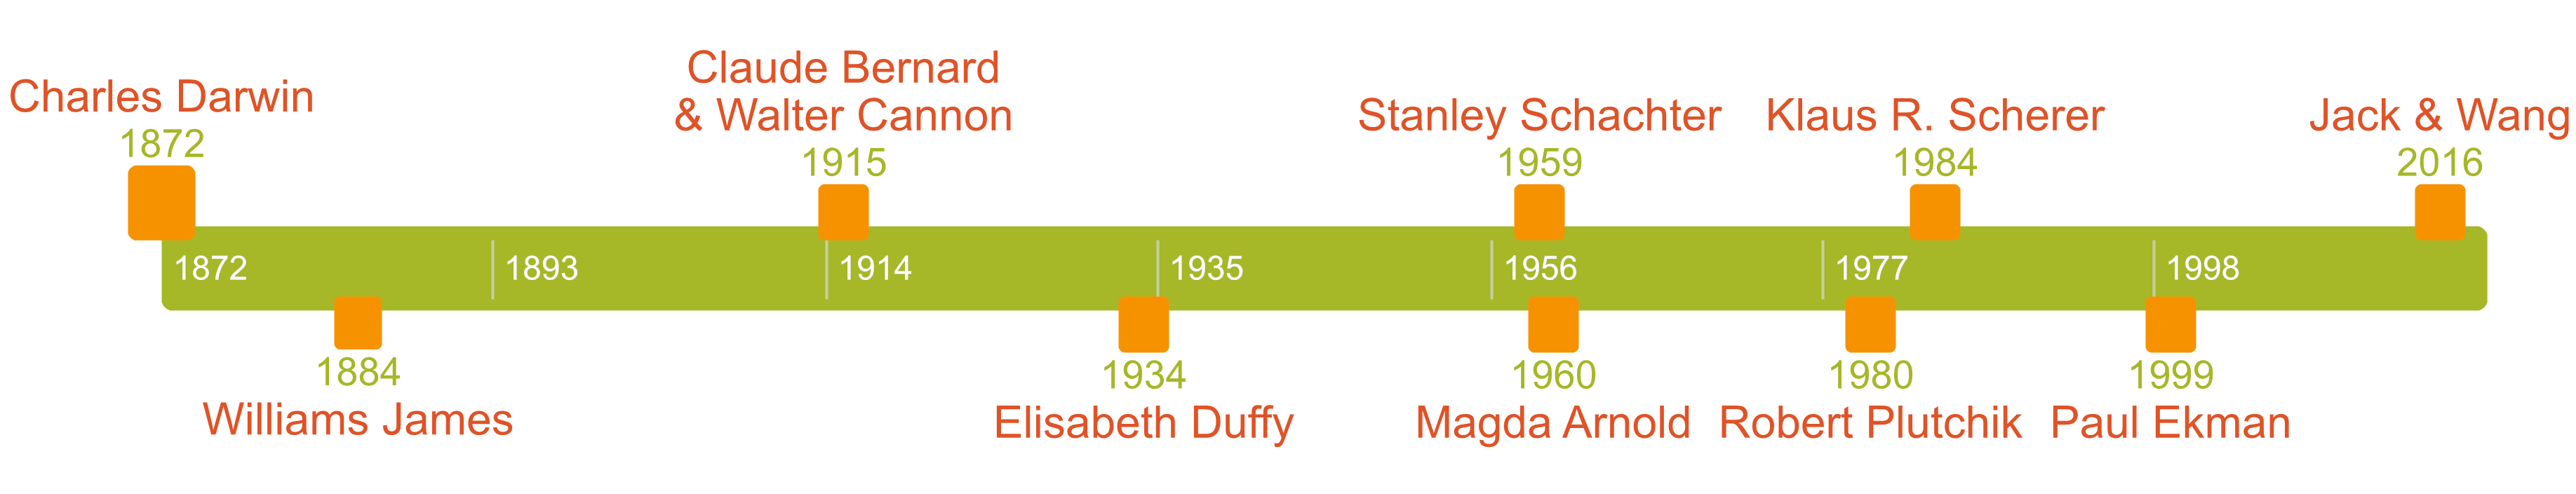
\includegraphics[width=16cm]{./Chapitre1/figures/friseHisto.png}
  \caption{Frise chronologique des grandes théories des émotions selon leur première date de parution}
  \label{fig:Circumplex}
\end{figure}


L'émotion et les états émotionnels, non content de ne pas avoir une unique définition, ont évolués dans leur caractérisation au fil du temps. Les premières mentions scientifiques de l'émotion nous viennent d'Aristote qui, au 4e siècle, définit l'Être comme une combinaison d'émotion et de raison. Bien plus tard, au 16e siècle, d'autres philosophes se sont intéressés à l'émotion tout en le mettant en relation avec la raison. Spinoza théorisait que les états émotionnels avaient une influence sur le raisonnement humain, tandis que Descartes pensait que ces deux notions étaient décorrélées.

\subsubsection{Les prémices de Darwin}
L'étude contemporaine des états émotionnels a réellement débuté avec les travaux de Darwin (1872)~\cite{Darwin1872}, qui a définit les sept principes régissant l'émotion:
\begin{itemize}
    \item les émotion sont innées : elles sont dues à l'Évolution et présentes dès la naissance. Elles se complexifient lorsque la personne grandit.
    \item elles suivent une continuité phylogénétique : les émotions sont aussi présentes chez les animaux proches de l'être humain, par exemple les primates.
    \item les émotions sont dénombrables : on peut caractériser chaque émotion par une des 8 catégories définies par Darwin (souffrances, abattement, joie, mauvaise humeur, haine, mépris, surprise et honte).
    \item elles sont analysables : on peut les caractériser en fonction de l'activité musculaire du visage.
    \item les émotions sont reconnaissables : les témoins reconnaissent l'émotion d'une personne en tant qu'information.
    \item elles sont universelles : comme elles viennent de l'Évolution, elles sont multi-culturelles et leur manifestation est reconnaissable par tous.
    \item elles sont actionnables : "le simple acte de simuler une expression tend à la faire naître dans notre esprit".
\end{itemize}
Les émotions servent donc à la survie de l’espèce et sont définies comme adaptatives. En effet, elles permettent d'adopter une réaction appropriée à un stimuli de l'environnement. Par exemple un danger se présente, concrètement un hippopotame. L'homme ressent une émotion en réponse à ce stimuli : la peur. Celle ci va activer toute une chaîne de réponses biologiques pour augmenter les chances de survie, notamment l'augmentation du rythme cardiaque pour mieux oxygéner les muscles et qui va permettre à l'homme de mieux attaquer ou fuir.
Darwin avance également que certaines émotions, les émotions basiques, sont universelles et innées. Elles sont donc à la fois ressenti et compris de tous. Cette notion d'émotion fondamentale va longtemps accompagner les théories visant à expliquer l'émotion, mais chaque contributeur définira leurs propres émotions primaires.

\subsubsection{L'émotion dite périphérique}
Avec la naissance de la psychologie, de nombreuses théories ont émergées pour définir et caractériser l'émotion. Williams James (1884) définit lui l'émotion comme une conséquence de la réponse physiologique à un stimuli de l'environnement~\cite{James1884}. L'émotion est dite "périphéraliste", ce qui était considéré auparavant comme la conséquence de l’émotion est ici avancé comme cause. Si une personne nous insulte, on ne crie pas parce qu'on est en colère, on est en colère parce qu'on crie. L'émotion se résumerait donc à la prise de conscience des changements qui s'opèrent dans notre corps (muscles, respiration, viscères...). Cela implique que les émotions sont contrôlables, on peut les accentuer ou les inhiber par le simple exercice de sa volonté. Bien que cette théorie soit en totale rupture avec les conceptions classiques de l'époque, elle va trouver un écho dans le siècle qui suivit et sera notamment partiellement validée par les travaux de James Douglas Laird (1974)~\cite{Laird1974} sur l'impact de l'expression faciale simulée dans le ressenti des émotions, de Stepper et Strack (1993) sur l'impact de la posture~\cite{Stepper1993} ou encore de Philippot (2002)~\cite{Philippot2002} sur l'impact de la respiration.

\subsubsection{L'émotion dite centrale}
En opposition à cette théorie, Claude Bernard et Walter Cannon (1915, 1927) vont définir la notion d’homéostasie~\cite{Cannon1915,Cannon1927}. Étudiant à l'époque le mouvement des viscères, il s'est rendu compte que ces dernières se contractées lorsque soumise à de vives émotions, allant jusqu'à constater l'arrêt de la digestion lors d'émotions suffisamment intense. L'émotion est un processus qui permet au corps d'interrompre son fonctionnement normal pour concentrer ses ressources dans une réponse adaptée, principalement l'attaque ou la fuite avec notamment la libération d'adrénaline dans le corps. L'émotion est donc centrale dans le corps, servant de système de mise en alerte de l'organisme.
%De plus, il met fin à l'idée que deux types de conduite peuvent être tenues par les mammifères et par extension par les hommes : soit on a des réactions immédiates (les réflexes), soit on a des réactions différées (réfléchis).
Ces travaux lui permettront également de situer la partie du cerveau responsable de l'émotion : les régions sous-corticales~\cite{Cannon1933}. Il décrit donc que ces régions sont responsables des réponses viscérales, c'est-à-dire des réponses homéostatiques d'urgence mais également du ressenti émotionnel de l'individu en tant qu'expérience subjective.
Les conclusions de ces travaux lanceront l'exploration du cerveau pour trouver les régions responsables des différentes émotions, amenant les neurosciences à s'emparer du domaine de l'émotion~\cite{Bard1934}.

\subsubsection{L'émotion sous forme d'activation}
En parallèle de ces explorations, la notion d'activation va émerger avec Élisabeth Duffy (1934, 1941)~\cite{Duffy1934,Duffy1941}. En effet, maintenant que les émotions sont détectables dans le cerveau humain, elles vont être traduites par des mesures du potentiel d'activité. La théorie des émotions en catégories comme définie par Darwin est donc réévaluée. En effet, si toutes les émotions peuvent être mesurées en potentiel d'activité de certaines zones du cerveau, la frontière entre les émotions peut être plus perméable que préalablement définie. Cette théorie inscrit donc un tournant dans l'étude des émotions, en introduisant des émotions plus complexes qui ne sont plus définit par un terme, une catégorie; mais par une mesure de potentiel sur une échelle donnée. Il s'agit là des prémices des théories dimensionnelles aussi appelées continues.
Cette théorie sera néanmoins plus difficile à démontrer que prévu, puisque les époux Lacey (1958) ont constaté que toutes les mesures (électro-encéphalogramme, activité des viscères, tension musculaires) ne covarie pas et sont différentes d'un individu à un autre~\cite{Lacey1958}.

\subsubsection{L'émotion en tant que théorie cognitivo-physiologique}
Suite à ce revers, Stanley Schachter (1959) a proposé sa théorie cognitivo-physiologique~\cite{Schachter1959,Schachter1962}. Selon lui, nous définissons nos émotions en fonction de la situation dans laquelle nous nous trouvons. En effet, nous devons raisonner pour définir nos propres émotions, en \textit{attribuant} celle-ci à un contexte interne ou externe. L'émotion naît donc de deux facteurs : l'activation physiologique et l'attribution cognitive. L'état émotionnel n'est donc plus une simple réponse à un stimulus de l'environnement, elle implique également une part de raisonnement.

\subsubsection{L'émotion avec la théorie de l'évaluation}
En s'appuyant sur ces travaux, Magda Arnold (1960) va amorcer la théorie de l'évaluation cognitive (appraisal en anglais)~\cite{Arnold1960}, qui va prendre de l'ampleur avec les travaux de Scherer (1984)~\cite{Scherer1984}. Ce dernier considère que l'évaluation d'une situation est définie par 5 questionnements :
\begin{itemize}
  \item Est-ce que la situation est nouvelle ? (nouvelle/ancienne)
  \item Est-ce qu'elle suscite du plaisir intrinsèque ? (agréable/désagréable)
  \item Est-ce qu'elle est pertinente ? (aidante/gênante)
  \item Est-ce qu'on sait y faire face ? (on a le contrôle/ on n'a pas le contrôle)
  \item Est-ce que c'est compatible avec les normes ? (compatible avec les normes sociales et ses propres convictions)
\end{itemize}
\begin{table}[]
\begin{tabular}{|l|l|l|l|l|}
\hline
\multicolumn{1}{|c|}{\textbf{Dimension d’évaluation}} & \multicolumn{1}{c|}{\multirow{2}{*}{\textbf{Colère/Rage}}} & \multicolumn{1}{c|}{\multirow{2}{*}{\textbf{Peur}}} & \multicolumn{1}{c|}{\multirow{2}{*}{\textbf{Tristesse}}} & \multicolumn{1}{c|}{\multirow{2}{*}{\textbf{Joie}}} \\
\multicolumn{1}{|c|}{\textbf{émotionnelle}}           & \multicolumn{1}{c|}{}                                      & \multicolumn{1}{c|}{}                               & \multicolumn{1}{c|}{}                                    & \multicolumn{1}{c|}{}                               \\ \hline
\multicolumn{5}{|c|}{\textbf{Nouveauté}}                                                                                                                                                                                                                                                  \\ \hline
Soudaineté                                            & haut                                                       & haut                                                & bas                                                      & bas                                                 \\ \hline
Familiarité                                           & bas                                                        & bas                                                 & bas                                                      & ouvert                                              \\ \hline
Prévisibilité                                         & bas                                                        & bas                                                 & ouvert                                                   & moyen                                               \\ \hline
\multicolumn{5}{|c|}{\textbf{Valence}}                                                                                                                                                                                                                                                    \\ \hline
intrinsèque                                           & ouvert                                                     & bas                                                 & ouvert                                                   & haut                                                \\ \hline
\multicolumn{5}{|c|}{\textbf{Rapport aux buts/besoins}}                                                                                                                                                                                                                                   \\ \hline
Pertinence                                            & haut                                                       & haut                                                & haut                                                     & moyen                                               \\ \hline
Degré de certitude dans la                            & \multirow{2}{*}{très haut}                                 & \multirow{2}{*}{haut}                               & \multirow{2}{*}{très haut}                               & \multirow{2}{*}{très haut}                          \\
prédiction des conséquences                           &                                                            &                                                     &                                                          &                                                     \\ \hline
Congruence avec les attentes                          & dissonant                                                  & dissonant                                           & ouvert                                                   & consonnant                                          \\ \hline
Opportunité                                           & obstruction                                                & obstruction                                         & obstruction                                              & facilitation                                        \\ \hline
Urgence                                               & haut                                                       & très haut                                           & bas                                                      & très bas                                            \\ \hline
\multicolumn{5}{|c|}{\textbf{Potentiel de maîtrise}}                                                                                                                                                                                                                                      \\ \hline
Causalité : agent                                     & autrui                                                     & autrui/naturel                                      & ouvert                                                   & ouvert                                              \\ \hline
Causalité : motivation                                & intentionnel                                               & ouvert                                              & hasard                                                   & intentionne                                         \\ \hline
Contrôle                                              & haut                                                       & ouvert                                              & très bas                                                 & ouvert                                              \\ \hline
Puissance                                             & haut                                                       & très bas                                            & très bas                                                 & ouvert                                              \\ \hline
Ajustement                                            & haut                                                       & bas                                                 & moyen                                                    & haut                                                \\ \hline
\multicolumn{5}{|c|}{\textbf{Accord avec les normes}}                                                                                                                                                                                                                                     \\ \hline
Standards externes                                    & ouvert                                                     & ouvert                                              & ouvert                                                   & ouvert                                              \\ \hline
Standards internes                                    & bas                                                        & ouvert                                              & ouvert                                                   & ouvert                                              \\ \hline
\end{tabular}
\label{tab:Scherer}
\caption{Grille d'évaluation des premiers travaux de Scherer pour définir une émotion en fonction des 5 questionnements. In P. Philippot. (2007). Emotion et psychothérapie (pp.11-64). La catégorie ouvert est utilisé lorsque l'évaluation peut etre de différente catégorie. Par exemple, pour la joie, l'élément déclencheur peut être quelque chose de connu ou non (Familiarité). En rapport aux buts/besoins, les opportunités peuvent être obstruées (émotions négatives) ou facilitées (émotions positives).}
\end{table}

C'est en réponse à ces 5 questions que Scherer va proposer 5 dimensions pour représenter l'émotion : la nouveauté, la valence, le rapport aux buts, le potentiel de maîtrise et l'accord avec les normes. La grille d'évaluation, présentée dans le tableau~\ref{tab:Scherer}, permet de caractériser l'état émotionnel d'un individu en 4 émotions : la colère/rage, la peur, la tristesse et la joie.
C'est en prenant appui sur toutes ces théories et ces travaux que le domaine de l'informatique va se mettre au service de l'étude de l'émotion.



\section{Représentation courante des émotions à but d'automatisation de traitement}
Comme nous l'avons vu précédemment, il n'y a pas de consensus sur une définition ou même une caractérisation des états émotionnels. Cela peut être expliqué par notamment, la multitude de domaines qui sont intéressées par l'émotion (psychologie, physiologie, linguistique, phonologie, sciences cognitives, informatique...) ou encore la part non négligeable de subjectivité du domaine.
Néanmoins dans le domaine de l'informatique, nous faisons principalement la distinction entre deux grands courants de théorie : l'émotion définit par des états discrets et/ou par des états continus. En effet, afin d'automatisation le traitement des émotions, il est nécessaire de se tenir à une théorie algorithmiquement descriptive, et donc de définir des représentations de l'émotion qui soient en adéquation avec les besoins exprimées par la tache à réaliser, ici la détection et la caractérisation automatique d'émotions contenus dans la parole. Nous proposons donc de rappeler la définition de ces deux ensembles de théorie qui sont "dans une guerre centenaire" l'une contre l'autre, donnant naissance à la multitude de définition que nous lui connaissons.

\subsection{Théorie des émotions discrètes}
La théorie des émotions discrètes considère qu'il existe un nombre déterminé d'émotions qui peuvent être formellement caractérisées. Certaines d'entre elles sont définies comme étant "basiques" ou "primaires" et permettent, en se combinant, d'exprimer des émotions plus "complexes". Elles sont caractérisées par ressenti spécifique et unique à chacun, des expressions comportementales et physiologiques elles aussi spécifique à chacun. Ces trois aspects permettent de caractériser chaque émotion. Certaines émotions sont admises par tous (peur, tristesse, joie, surprise, dégoût, colère), d'autres sont plus discutées~\cite{Cosnier1994}.
Darwin est l'un des premiers à définir ces émotions basiques, au nombre de 5 (la colère, la peur, la tristesse, le dégoût et la joie), dans sa théorie de l'évolution où il explique que les émotions sont nécessaires à la survie de l'homme, ce qui expliquerait notamment pourquoi elles ont une influence sur notre biologie, nous permettant également de les reconnaître.
Comme a dit Izard : "people need the category label of fear to explain flight to one another for safety, anger to explain the frustration of blocked goal responses, joy (or its equivalent) to explain the pride of achievement, and sadness to explain the experience of a life-changing loss"~\cite{Izard2007}.
Cependant il n'y a pas de théorie principale qui permettrait de définir ces émotions basiques, de les dénombrer ou d'expliquer leur combinaison en émotions complexes. D'autant plus que les émotions et leur manifestation n'ont pas cessé d'évoluer en fonction des évolutions de nos sociétés.

\begin{table}[]
\begin{tabular}{|l|l|}
\hline
\textbf{Auteyrs} & \textbf{Émotions basiques} \\ \hline
Darwin (1872)       & colère, peur, joie, tristesse, dégoût                                                               \\ \hline
James (1884)        & peur, douleur/chagrin, amour, rage                                                                  \\ \hline
Arnold (1960)       & \begin{tabular}[c]{@{}l@{}} colère, aversion, haine, peur, découragement, \\
                              courage, amour, désir, espoir, désespoir, tristesse\end{tabular}                            \\ \hline
Tomkins (1962)      & rage, peur, joie, angoisse, dégoût, surprise , intérêt, honte                                      \\ \hline
Izard (1971)        & \begin{tabular}[c]{@{}l@{}} intérêt, joie, surprise, tristesse, colère, dégoût, mépris, \\
                              auto-hostilité, peur, honte, timidité, culpabilité \end{tabular}                            \\ \hline
Plutchik (1980)     & \begin{tabular}[c]{@{}l@{}} colère, peur, joie, tristesse, dégoût, surprise,  \\
                              acceptation, anticipation \end{tabular}                                                     \\ \hline
Frijda (1986)       & désir, intérêt, bonheur, surprise                                                                   \\ \hline
Oatley \& Jonhson-Laird (1987)    & colère, dégoût, inquiétude, bonheur, tristesse                                        \\ \hline
Gray (1990)         & rage, terreur, anxiété, joie                                                                        \\ \hline
Ekman (1999)        & colère, peur, joie, tristesse, dégoût, surprise                                                     \\ \hline
\begin{tabular}[c]{@{}l@{}}Jack (2016), Gu (2015)
  \\ et Wang (2016)\end{tabular}   & peur, colère, joie, tristesse                                                        \\ \hline
\end{tabular}
\label{tab:EmotionsBasiques}
\caption{Définition des émotions basiques selon différents auteurs}
\end{table}


De nombreux auteurs ont proposés des émotions primaires : Paul Ekman propose les populaires 6 émotions basiques (la peur, la colère, la joie, la tristesse, le dégoût et la surprise) qu'on appellera par la suite les "Big Six"~\cite{Ekman1999}, tandis que Plutchik en propose 8 (la colère, la peur, la tristesse, le dégoût, la surprise, l'anticipation, la confiance et la joie)~\cite{Plutchik1980}. Jack, Gu et Wang~\cite{Jack2016,Gu2015,Wang2016} ont quand à eux proposés 4 émotions basiques (la peur, la colère, la joie et la tristesse). Le tableau~\ref{tab:EmotionsBasiques} liste, en partie, les définitions des émotions primaires selon leurs auteurs.

Paul Ekman a joué un grand rôle dans la diffusion de cette théorie grâce, entre autre, à la création de la méthode "Facial Action Coding System" (FACS)~\cite{Ekman1978} utilisée dans des domaines grand public tel que la série Lie to Me. Il a notamment décrit les 9 caractéristiques d'une émotion basale~\cite{Ekman1992} qui sera globalement repris par tous les autres auteurs :
\begin{itemize}
  \item Les signaux émotionnels sont universels : les émotions de base sont reconnues par tout le monde, quelque soit sa culture ou son origine.
  \item Il existe des expressions communes aux hommes et aux autres primates : nous sommes capables d'identifier la colère chez les Bonobos par exemple.
  \item Chaque émotion est caractérisée par un ensemble de comportements physiologiques comme exprimé par la figure~\ref{fig:Ekman1983}.
  \begin{figure}
  \centering
  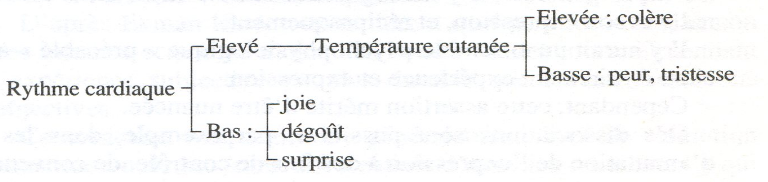
\includegraphics[width=10cm]{./Chapitre1/figures/Ekman1983.png}
  \caption{Traduction de la figure extraite de l'article de Paul Ekman et al.~\cite{Ekman1983} décrivant un arbre de décision pour déterminer l'émotion retrouvée sur le visage.}
  \label{fig:Ekman1983}
\end{figure}

  \item Il existe des éléments déclencheurs d'émotion qui sont universels : controversée, cette caractéristique stipule que des types de situations données provoqueront une émotion données chez tout sujet.
  \item Les réactions émotionnelles sont cohérentes : il y a un lien établi et connu entre une expérience émotionnelle et son expression physiologique et réciproquement.
  \item L'émotion engendre une réaction rapide : une fraction de seconde pour les réactions physiologiques et quelques millisecondes pour les mimiques~\cite{Ekman1978}.
  \item L'émotion est limitée dans le temps : la durée d'une émotion n'excède pas la minute.
  \item L'émotion n'est pas contrôlée : une émotion frappe soudainement, n'étant ni volontaire ni raisonnée. Un individu peut essayer de contrôler les manifestations de l'émotion. La posture et les mimiques sont plus contrôlables que la voix. Les réactions viscérales sont quant à elle très peu contrôlables.
  \item L'émotion est spontanée : elle n'est pas choisie et ne peut pas vraiment être éviter. Toutefois son anticipation peut réduire son intensité. Par exemple devant un film d'horreur, on s'attend à avoir peur, ce qui permet de réduire cette peur.
\end{itemize}

\begin{figure}
  \centering
  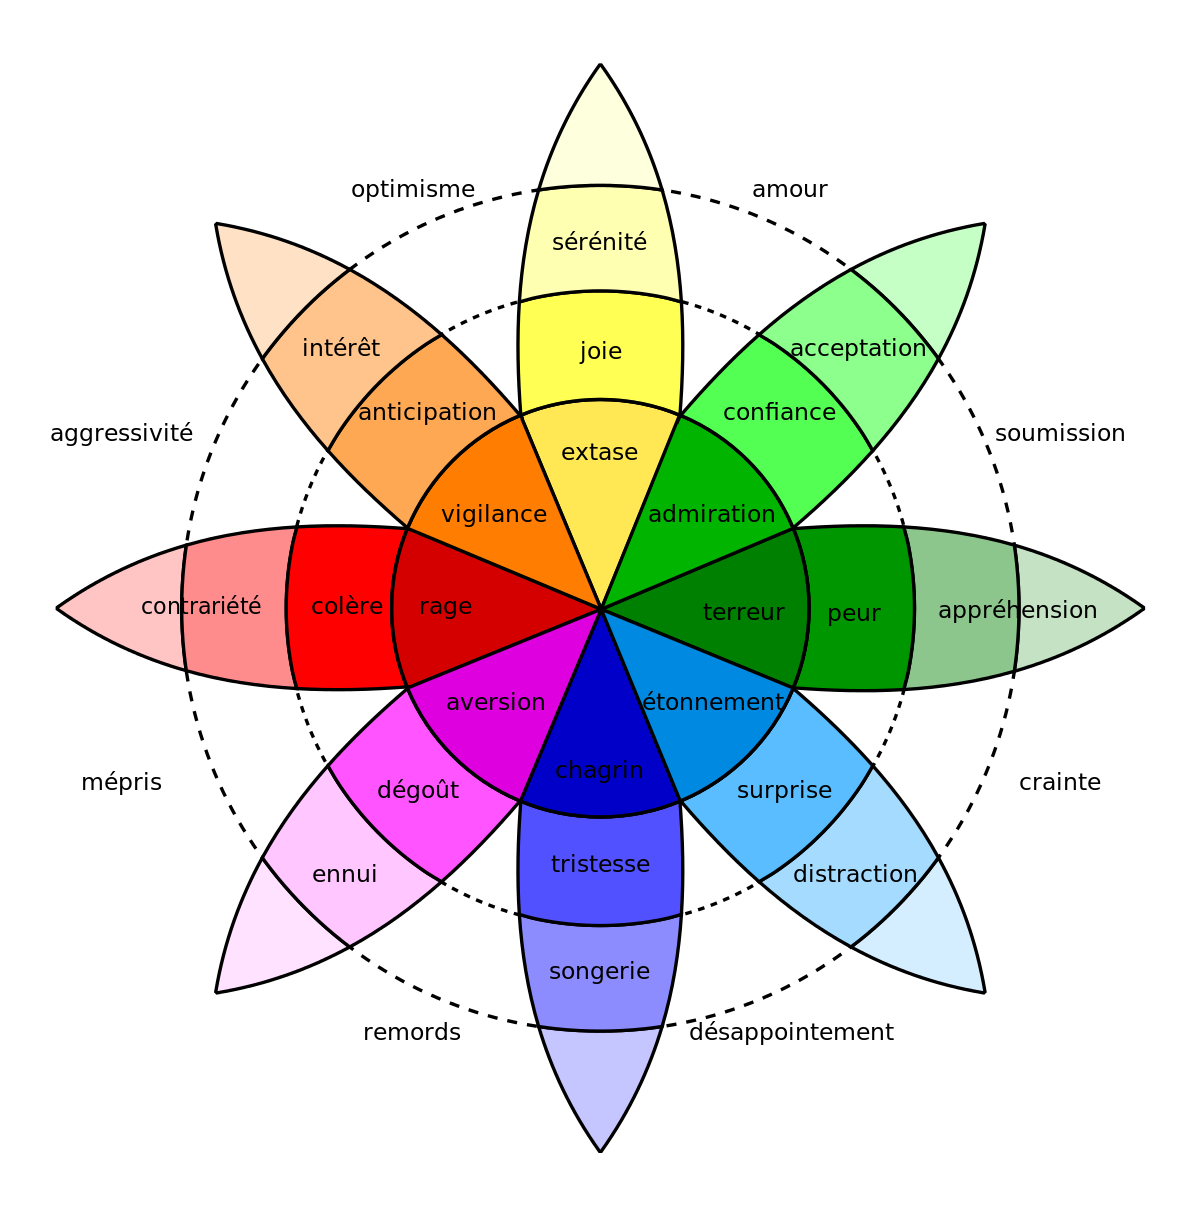
\includegraphics[width=12cm]{./Chapitre1/figures/Plutchik.png}
  \caption{Roue de Plutchik qui définit les émotions complexes à partir d'émotions basiques.}
  \label{fig:Plutchik}
\end{figure}


Ces émotions primaires peuvent également se combiner pour donner des émotions dites "complexes", qui permettent de nuancer les états émotionnels. C'est notamment le cas avec la roue de Plutchik, présentée dans la figure~\ref{fig:Plutchik}, qui dénombre 32 émotions caractérisées en 8 émotions primaires selon leur intensité~\ref{Plutchik1980}. De plus, on parle également d'émotions secondaires afin de décrire des émotions qui ne sont pas innées, mais qui sont apprises pendant le développement de la personne. Paul Ekman définit ainsi 9 émotions secondaires, plus complexes et plus difficiles à identifier (la culpabilité, l'embarras, le mépris, la complaisance, l'enthousiasme, la fierté, le plaisir, la satisfaction et la honte) qui sont marquent des différences d'expression en fonction des cultures et des individus. Charland (1995)~\cite{Charland1995} et Damasio (1999)~\cite{Damasio1999} ont notamment contribué à analyser les différences culturelles de ces émotions secondaires.
En plus de ces théories discrètes, l'émotion peut être définie par de nombreuses théories continues.

\subsection{Théorie des émotions continues}

\begin{figure}
  \centering
  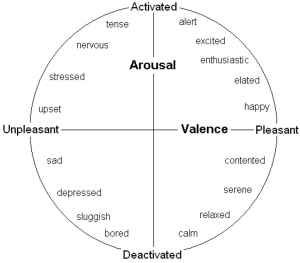
\includegraphics[width=8cm]{./Chapitre1/figures/Circumplex.png}
  \caption{Le modèle circumplex de Russell}
  \label{fig:Circumplex}
\end{figure}

Dans la vie courante, il est bien plus facile et coutumier de se référer à des catégories d'émotion tel que la joie ou la tristesse pour décrire ce que l'on ressent. Toutefois, une autre façon de définir les émotions est de les inscrire dans des espaces continus, permettant de s'affranchir des contraintes de ces catégories définies. Si l'on s'en réfère aux travaux de Feldman-Barrett (2006)~\cite{Feldman2006} , ces catégories «représente(nt) maintenant un obstacle majeur à la compréhension de ce que sont les émotions et de comment (les émotions) fonctionnent».
La théorie des émotions continues, aussi appelée émotions en dimensions, a été introduit par les travaux de Wundt (1902)~\cite{Wundt1902} et Schlosberg (1954)~\cite{Schlosberg1954}. Les émotions sont descriptibles selon trois dimensions indépendantes nommées en fonction de leur extremum : agréable-désagréable, tendu-détendu et agité-calme. Grace à ces trois dimensions, chaque émotion ressentie par un individu peut être décrite comme une combinaison pondérée de ces trois axes.  Comme ces dimensions se chevauchaient, ces dernières ont été remplacées par le modèle du Circumplex, présentée dans la figure~\ref{fig:Circumplex}, de Russell en 1980~\cite{Russell1980}, devenant la théorie principale permettant de décrire les émotions de façon continue. Ce modèle permet de placer toutes les émotions au sein d'un cercle dont l'abscisse définit la valence de l'émotion (positive-négative) et l'ordonnée définit l'activation (faible-fort). En effet, on peut donc donner une polarité et une intensité à chaque émotion. Afin de mieux discriminer des émotions qui avaient des mêmes valeur de valence et d'activation comme par exemple la peur et la colère, d'autres axes ont également été ajoutées sur ce modèle par Scherer (2005) comme la dominance (dominance-soumission), l'imprévisibilité (faible-forte)~\cite{Scherer2005}, comme illustré dans la figure~\ref{fig:Genova}. Par exemple, on peut voir que la mélancolie (melancholic) a une valence neutre et une faible activation, tandis que la déception (disappointed) a une valence très négative et une activation neutre.
\begin{figure}
  \centering
  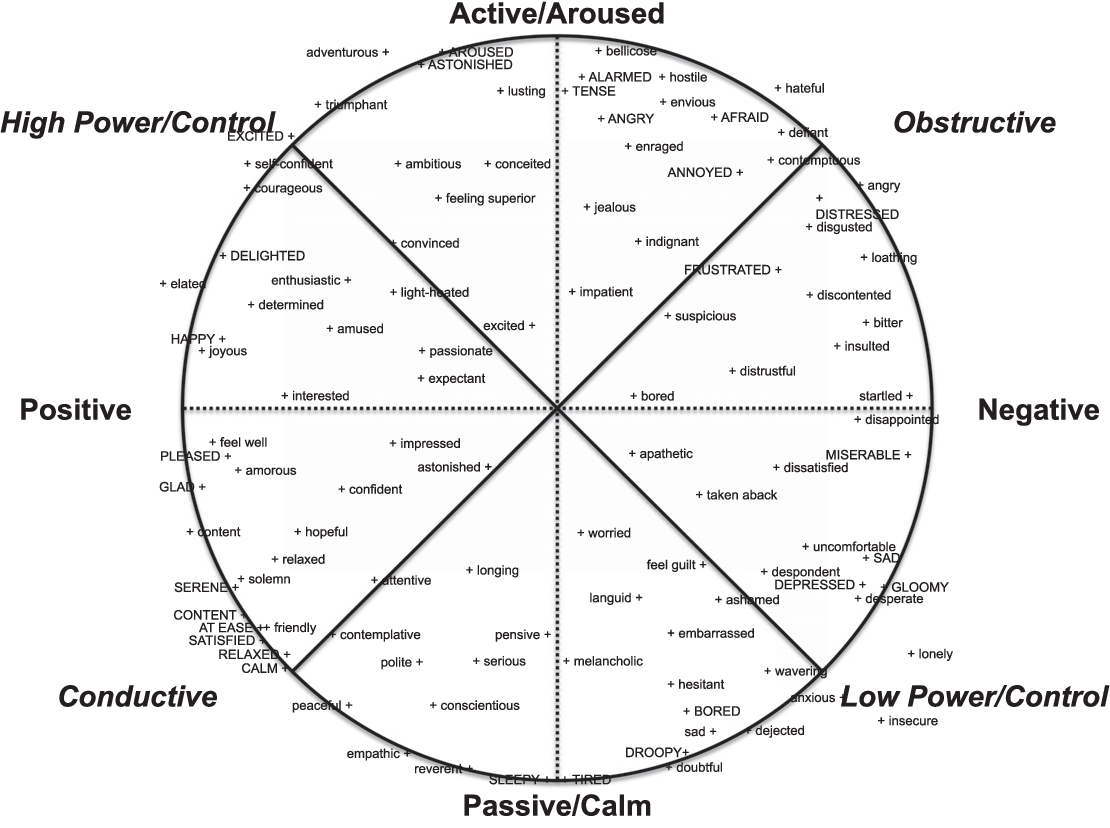
\includegraphics[width=18cm]{./Chapitre1/figures/Genova.png}
  \caption{La roue des émotions de Genève définie par Scherer, qui nomme des émotions (primaires ou secondaires) dans des dimensions continues.}
  \label{fig:Genova}
\end{figure}

D'autres systèmes dimensionnelles existent, allant de 2 dimensions à 5 dimensions, qui ont été crée en fonction des besoins applicatifs. Toutes ces dimensions peuvent être discrétisées par des systèmes de graduations, permettant notamment de faire le lien avec les théories discrètes.
En ce qui concerne les études menées sur les émotions continues dans le domaine de l'informatique, il y a une forte prévalence des dimensions de valence et d'activation quelque soit le support utilisé (la voix, le texte, la vidéo ou des données physiologiques). En effet, elles sont facilement identifiables par l'humain et reposent sur des caractéristiques automatiquement reconnaissables. Au sein de cette thèse, nous avons décidé de nous appuyer sur la théorie des émotions continues, afin de répondre à la problématique industrielle.


\section{L'émotion dans la parole : para-linguistique et prosodie}
Si nous nous replaçons dans le contexte de cette thèse, notre objectif est de décrire l'émotion humaine lors de conversations tenues entre un client et un agent dans un cadre défini par un appel téléphonique en centre d'appels. Nous n'avons donc que la voix comme axe d'analyse pour en retirer les états émotionnels des intervenants.
La voix, produite par l'appareil phonatoire humain, que l'on considère comme un canal de communication comme définit par Shannon (1948)~\cite{Shannon1948}, permet de faire passer un message entre un émetteur (ici le locuteur) et un récepteur (ici l'écoutant) grâce à son appareil auditif.

Ces deux appareils sont la base de la communication orale entre deux individus. L'appareil phonatoire décrit l'ensemble des phénomènes anatomiques qui sont impliquées dans la production des vibrations acoustiques donnant naissance à la parole. Par exemple, la création d'un son par la vibrations des cordes vocales ou encore la modulation de ce son par la bouche et le nez. La parole peut etre découper en sous unité phonique que l'on appelle des phonèmes. Ces derniers, à ne pas confondre avec des syllabes, permettent de composer l'ensemble des sonorités nécessaires à l'énonciation de parole.
%Par exemple, le mot 'émotion' utilise 6 phonèmes : /e/ (é), /m/ (m), /ɔ/ (o), /s/ (s), /i/ (i) et /ɔ̃/ (on).
Le langage étant directement influencé par la langue parlée par le locuteur, chaque langue possède sa propre palette de phonèmes. Le français par exemple utilise 37 phonèmes, tandis que le japonais n'en utilise que 22.
L'appareil auditif quant à lui, est composé de tout ce qui permet à l'individu d'entendre et d'écouter la parole. Il est notamment composé de l'oreille mais également du cerveau, qui est un acteur de la perception auditive. Pour ce qui est de l'oreille, elle se compose de trois parties :
\begin{itemize}
  \item l'oreille externe : conduit qui permet de transmettre les vibrations acoustiques
  \item l'oreille moyenne : transforme le signal pour qu'il puisse être conduit dans un environnement liquide en utilisant les osselets,
  \item l'oreille interne : transforme les vibrations en influx nerveux grâce à la cochlée.
\end{itemize}
C'est cet appareil qui permet à un interlocuteur de recevoir un message.

Les informations communiquées par ce canal peuvent être notamment divisées en deux catégories, la linguistique et le para-linguistique.
Le linguistique va décrit le langage en tant que parole de base tandis que le para-linguistique va définit tout ce qui n'est pas du message verbal. Par exemple, dans la vie de tous les jours, "Bonjour, je voudrais une baguette de pain" correspond au message linguistique, tandis que le sourire, le geste de la main, l'hésitation vocale ou le raclement de gorge fera partie du domaine para-linguistique.
Shirley Weitz (1974)~\cite{Weitz1974} explique que la paralinguistique s'intéresse "à la façon dont quelque chose est dit, pas à ce qui est dit". Globalement, on considère du domaine du para-linguistique dans la parole, l'accent, la hauteur, le volume, la vitesse de parole, la modulation, la prosodie et la fluidité de l'élocution.
La définition du paralangage étant évolutive, il est donc naturellement que sa définition reste imprécise comme l'indique Peter Matthews dans son dictionnaire de la linguistique~\cite{Matthews2014}.
La prosodie est défini par l'ensemble des phénomènes qui accompagnent le discours, tout en n'étant pas du discours. Elle est notamment marquée par trois paramètres très important:
\begin{itemize}
  \item La fréquence fondamentale (F0) de la parole correspond à l'inverse de la période d'un son périodique, c'est à dire à la durée des sons de type voyelles dans la parole,
  \item La rythme de la parole qui correspond au temps nécessaire à l'émission d'un segment de parole,
  \item l'intensité de la parole qui est définit par l'énergie contenue dans le signal.
\end{itemize}
C'est par l'étude para-linguistique et de la prosodie que nous analysons notamment inconsciemment le discours d'un locuteur afin de déterminer son état émotionnel. Comme il s'agit du sujet principal de cette thèse, le chapitre~\ref{chapitre3} revient plus en détail sur la relation entre la voix et les émotions. Mais la voix n'est pas la seule modalité véhiculant des indices émotionnels.

\subsection{Satisfaction et frustration dans la voix}

\section{L'émotion dans le texte}
Utiliser le texte pour déterminer l'état émotionnel est une voie de plus en plus empruntée grâce, notamment, à la performance des systèmes de reconnaissance de la parole actuel.
Si des domaines comme l'Affect analysis ou la détection d'opinion utilise des données textuelles de type livres, témoignages ou plus récemment tweets et contenus en ligne afin d'extraire des états émotionnels, on peut également considérer la transcription automatique comme un élément dissocié de la parole, et donc y retrouver des marqueurs de l'émotion. Rappelons que l’analyse de sentiments désigne plutôt l’analyse en polarité positif-négatif de l'occurence, tnadis que l'opinion est généralement décrites en trois catégories "bien/neutre/mal".On cherche alors l'émotion dans l'aspect sémantique de la phrase, dans les diffluences ou les répétitions.
Des outils tel que des dictionnaires de polarité permettent de colorer émotionnellement des mots ou des phrases, ou encore des postagger permettant d'étudier la structure d'un énoncé pour faire ressortir sa forme morphosyntaxique sont utilisés dans la reconnaissance d'émotions que ce soit à l'échelle d'un segment de parole, d'une phrase ou d'un document.

\subsection{Satisfaction et frustration dans le texte}

\section{Les autres indices émotionnels chez l'humain}
Outre la présence de marqueurs émotionnelles dans la voix, d'autres indicateurs peuvent être relevées dans notamment les expressions faciales et les signaux physiologiques. Il est donc possible d'étudier l'état émotionnel d'une personne à partir d'une vidéo ou de relevés cardiaques par exemple.

\subsection{Les marqueurs faciaux et comportementaux de l'émotion}

\begin{figure}
  \centering
  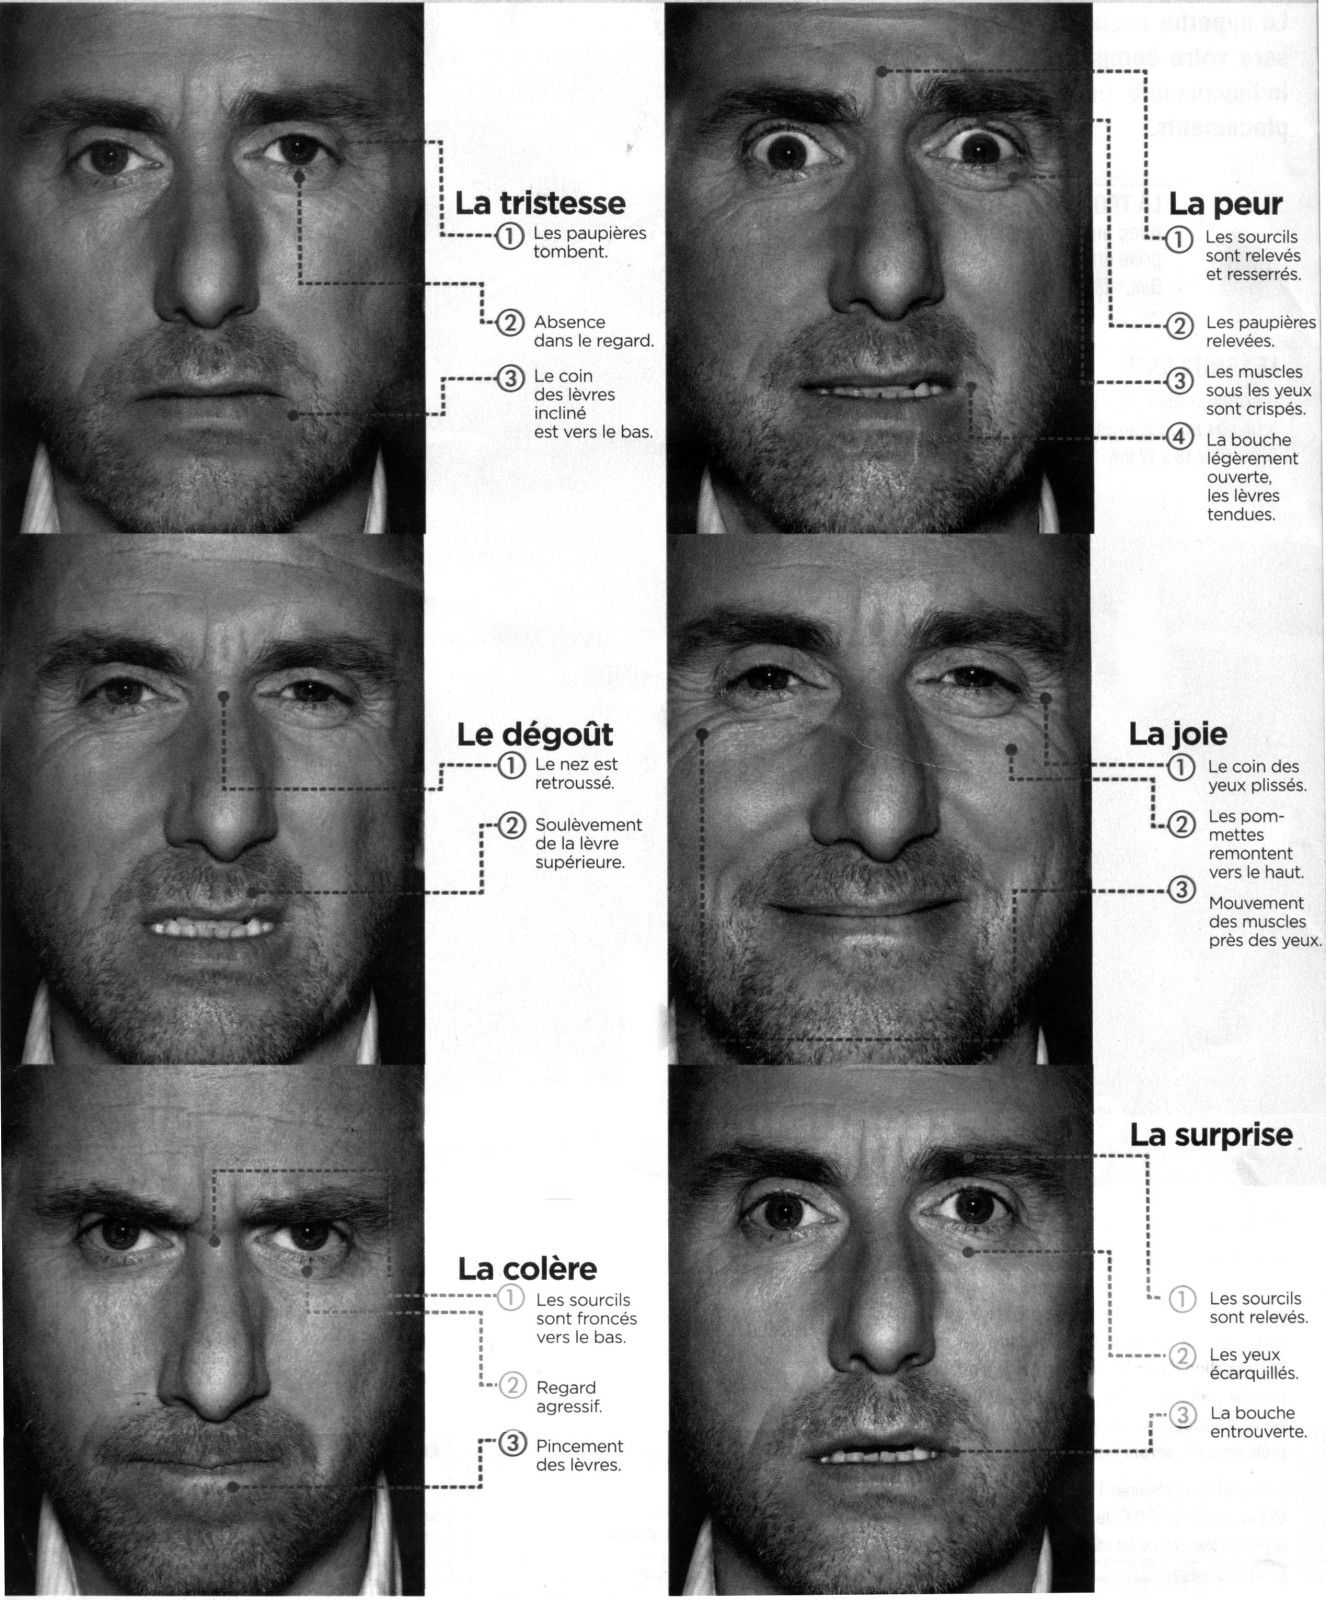
\includegraphics[width=14cm]{./Chapitre1/figures/ExpressionFacial.jpg}
  \caption{Marqueurs faciaux des 6 émotions primaires d'Ekman. In Lie To Me.}
  \label{fig:expressionFacial}
\end{figure}

Il est possible de capter beaucoup d'information sur le visage et dans l'attitude d'une personne. Nos expressions faciales notamment permettent de véhiculer les émotions primaires tel que la peur ou la colère~\ref{fig:expressionFacial} en mettant en jeu le positionnement des sourcils, la forme de la bouche, le plissement du front... Bien qu'affirmé comme étant universelles par Paul Ekman~\cite{Ekman1978}, de nombreuses études ont mis en doute ce postulat. En effet, certains indicateurs étant communs entre plusieurs émotions, des interlocuteurs peuvent se tromper dans l'analyse de l'émotion de la personne. Par exemple, la bouche ouverte peut signifier la peur mais également la surprise. Les expressions faciales sont également contrôlables. En effet, il est tout à fait possible de simuler une émotion ou dans une moindre mesure, d'en cacher une selon l’entraînement d'un individu.
Malgré ces inconvénients, les expressions faciales sont, aujourd'hui encore, l'une des modalités les plus observées pour définir et reconnaître des émotions. Elles peuvent également servir à détecter des états dépressifs ou des mensonges par exemple.

L'attitude d'une personne permet également de reconnaître ces émotions. En effet, les comportements adoptés par un individu, notamment la posture, peuvent refléter de l'état émotionnel interne d'une personne. Ce phénomène est expliqué dans les travaux de Fijda (1987)~\cite{Fijda1987} qui indique que les émotions sont la pour aider l'homme à agir : l'homme est caractérisé par une tendance à l'action qui se traduit par des émotions. Ainsi lors de la colère, la position du buste du corps sera en avant, tandis que pour la peur, elle sera recroquevillée sur elle-même. Mais ces marqueurs faciaux et comportementaux ne sont pas les seuls marqueurs utilisables.

\subsection{Les marqueurs physiologiques de l'émotion}
Comme nous l'avons vu précédemment, l'expression de l'émotion est étroitement liée au cerveau et donc au système nerveux. En étudiant ce dernier, nous pouvons retrouver des marqueurs émotionnels. La peur par exemple, engendre une augmentation du rythme cardiaque, qui va augmenter l'afflux sanguin, de la sudation, l'augmentation de l'apport en oxygène par une respiration plus rapide. De manière non-exhaustive, nous pouvons citer le rythme cardiaque, la sudation, la température de la peau (à l'origine des joues rouges), l'activité cérébrale, le suivi du regard, le rythme de la respiration comme des marqueurs physiologiques de l'émotion. Certains de ces marqueurs physiologiques peuvent être quantifiés par des outils de mesure. L'électrocardiogramme (EG) permet de suivre l'évolution du rythme cardiaque, l'électroencéphalogramme (EEG) permet de détecter les zones d'activités du cerveau. Des capteurs de sudation et des thermomètres peuvent permettre de suivre la production de sueurs au niveau des main ou la température corporelle. Tous ces indicateurs peuvent caractériser la présence ou l'absence d'émotion chez un individu ainsi que la caractériser.


\clearemptydoublepage

\chapter[ceci est un long titre]{Nom du chapitre 2}

Lorem ipsum dolor sit amet, «~consectetuer~» adipiscing elit. Maecenas fermentum, elit non lobortis cursus, orci velit suscipit est, id mollis turpis mi eget orci. Ut aliquam sollicitudin metus. Mauris at sapien sed sapien congue iaculis. Nulla lorem urna, bibendum id, laoreet iaculis, nonummy eget, massa. Phasellus ullamcorper commodo velit. Class aptent taciti sociosqu ad litora torquent per «~conubia nostra~», per inceptos hymenaeos. Phasellus est. Maecenas felis augue, gravida quis, porta adipiscing, iaculis vitae, felis. Nullam ipsum. Nulla a sem ac leo fringilla mattis. Phasellus egestas augue in sem. Etiam ac enim non mauris ullamcorper scelerisque. In wisi leo, malesuada vulputate, tempor sit amet, facilisis vel, velit. Mauris massa est, sodales placerat, luctus id, hendrerit a, urna. Nullam eleifend pede eget odio. Duis non erat. 


\clearemptydoublepage
\chapter{Reconnaissance automatique des émotions : corpus et méthodes}
\label{chapitre3}
«Si vous voulez être libre de vos émotions il faut avoir la connaissance réelle, immédiate de vos émotions.»  (Arnaud Desjardins, 1925-2011)


\section{Le domaine de la reconnaissance automatique des émotions}
Le domaine de la reconnaissance automatique des émotions, ou Speech Emotion Recognition (SER) se concentre sur les tâches de reconnaissance des différents états émotionnels d'un ou de plusieurs locuteurs. Ce domaine est en pleine expansion grâce notamment à l'utilisation de nouveaux systèmes neuronaux empruntés à d'autres domaines du Machine Learning.
Afin de mettre en place des expérimentations sur ces tâches de reconnaissance et de caractérisation des émotions, il est important de mettre en place des données pertinentes sur lesquelles s'appuyer, des méthodes pour représenter efficacement ces données ainsi que de mettre en place des systèmes d'évaluation robustes permettant de comparer les différentes expérimentations.

\section{Les corpus existants}
Aujourd'hui, les tâches de reconnaissance d'émotion sont principalement traitées en tant que tâches supervisées : le système apprend à reconnaître des étiquettes émotionnelles associées à des segments de parole à partir de corpus de parole annotés en émotions.

\subsection{Les différents types de corpus}
\subsubsection{Corpus actés}
Comme nous l'avons vu dans le premier chapitre de cette thèse, la caractérisation de l'état émotionnel d'une personne peut être assez délicate, puisqu'elle est en grande partie subjective. De plus, il est communément admis que l'expression des états émotionnels sont ponctuels et rares dans la parole. Pour pallier ce problème, on peut construire des corpus dit \textit{actés}. Il s'agit de corpus où l'état émotionnel n'est pas naturel.

On fait alors appel à des acteurs, qui vont simuler des états émotionnels dictés par le responsable de l'élaboration du corpus. Par exemple, les acteurs devront dire le mot \textit{hippopotame} de façon joyeuse, triste puis avec dégoût. Cette pratique est très utilisée pour avoir différents états émotionnels d'un même locuteur, le tout rapidement. Elle est à privilégier quand on recherche l'exhaustivité des états émotionnels chez un sujet. Ces corpus sont aujourd'hui toujours majoritaires. On peut notamment citer les corpus Emo-Db~\cite{Burkhardt2005} et DES~\cite{Engberg1997}. L'inconvénient principal d'un tel protocole est que les émotions obtenues sont prototypiques dans leur manifestation, les rendant difficile à comparer à des émotions dites \textit{naturelles}. De plus, l'utilisation d'acteurs peut se révéler coûteuse.

\subsubsection{Corpus induits}
Un autre type de corpus utilisé dans la reconnaissance d'émotion est le corpus induit. On utilise différentes méthodes pour induire les états émotionnels que l'on souhaite étudier.

Une des méthodes pour construire ce genre de corpus est d'utiliser un \textit{magicien d'Oz} abrégé WoZ (\textit{Wizard of Oz}). Cette méthode consiste à simuler un dialogue homme-machine, où la machine est en fait complètement commandée par un opérateur humain, qui va simuler une réponse de machine. Ainsi l'humain pense avoir affaire à un serveur vocal ou un robot, alors que c'est l'opérateur qui est responsable des réponses engendrées par le système.

On peut également parler de la recherche de stress par laquelle on peut placer les sujets dans des situations stressantes comme des montagnes russes~\cite{Hansen1997} ou une prise de parole en public~\cite{Giraud2013}. Quant à la tristesse, on peut utiliser des extraits de films par exemple~\cite{Schuller2010cinemo}. Ces émotions sont plus proches des émotions réelles, elles sont donc moins manifestes.

Les corpus actés et induits ont pour avantage d'être créés dans des environnements contrôlés et permettent de rendre les données facilement accessibles. Ces données sont, la plupart du temps, produites à des fins d'analyse. Il est donc facile de recueillir le consentement des participants avant la mise en place de l'expérience, de contrôler la qualité des enregistrements et la cohérence des données en contraignant les participants sur un sujet ou à exprimer un type d'état émotionnel défini. Néanmoins ils ne représentent pas la vie réelle, sont souvent de petite taille et sont difficilement fusionables pour permettre d'avoir une plus grande quantité de données.

\subsubsection{Corpus naturels}
Les corpus non actés, aussi appelés naturels ou \textit{real-life} sont obtenus directement à partir de données issues de la vraie vie. Ils proviennent d'environnements peu ou pas contrôlés où les participants n'ont pas connaissance de leur implication dans l'expérimentation a priori. On peut travailler par exemple avec des enregistrements provenant de débats télévisés, de reportages, de vidéos internet ou de centres d'appels. Ces données sont donc constituées d'états émotionnels spontanés. Les émotions y sont souvent moins marquées et moins prototypiques que des émotions actées. De plus la parole spontanée contient une grande part de parole neutre non expressive, et la présence d'émotions reste peu fréquente.

Ces corpus sont difficiles à construire et à diffuser : soit les participants doivent être retrouvés et ils doivent donner leurs consentement a posteriori, soit les données doivent être anonymisées pour respecter la réglementation générale sur la protection de données (RGPD). De même, il est difficile d'avoir tous les états émotionnels de tous les locuteurs et de garantir une qualité d'enregistrement identique entre tous les documents.
De plus, l'étiquetage de ces données est souvent plus complexe, puisque le cadre expérimental n'a pas été expliqué aux participants.

\subsection{Les différents types d'acquisition}
L'acquisition des enregistrements est un paramètre important dans la catégorisation des corpus. En effet, un ensemble d'enregistrements captés par un micro spécifique ne donnera pas la même qualité acoustique qu'une voix téléphonique.

On retrouve plusieurs types d'acquisition :
\begin{itemize}
  \item Acquisition en labo : le milieu d'acquisition est contrôlé par les responsables du corpus. Cela permet une homogénéité entre les différents enregistrements. On peut notamment citer le corpus SEWA~\cite{SEWA}.
  \item Acquisition en studio : les données sont acquises par des studios de radio ou de télévision. Par exemple MSP-Podcast~\cite{Lotfian2019} regroupe des enregistrements de podcast, réalisés en studio.
  \item Acquisition en conditions réelles : le milieu d'acquisition est peu contrôlé par les responsables du corpus. Ce genre d'acquisition est prépondérante dans les corpus naturels. On peut citer notamment les corpus comportant des conversations de centres d'appels comme CallSurf~\cite{Garnier2008} ou Natural~\cite{Morrison2007}, de conversations téléphoniques d'urgence~\cite{Devillers2010} ou bien de micro trottoir ou d'enregistrements de conversations dans des lieux publics comme ESLO~\cite{Eshkol2011}.
\end{itemize}

\subsection{Les différents types d'annotation}
Dans le chapitre précédent, nous avons vu différentes théories émotionnelles. La plupart des travaux du domaine se basent principalement soit sur les catégories discrètes d'émotions, soit sur les dimensions émotionnelles, soit une combinaison des deux. Ainsi  suivant la théorie utilisée, les données émotionnelles présentes dans les corpus collectés se fait donc généralement soit suivant une annotation discrète, soit sur une annotation continue, en respectant un schéma d'annotation qui lui est propre. Cette variabilité dans les protocoles d'annotation ne facilite pas l'utilisation jointe de plusieurs corpus pour construire des systèmes de reconnaissance d'émotion appris sur de plus grandes quantités de données.

Pour garantir la qualité de l'annotation, plusieurs indicateurs sont à notre disposition, notamment le kappa (qui mesure un accord annotateur sur plusieurs classes) ou le coefficient de corrélation (qui mesure un accord annotateur sur une dimension). Ces deux méthodes sont décrites dans le prochain chapitre.

\subsection{Synthèse}

\begin{table}[]
\begin{tabular}{|l|c|c|c|c|l|}
\hline
\textbf{Nom du Corpus}                              & \multicolumn{1}{l|}{\textbf{Langue}} & \multicolumn{1}{l|}{\textbf{Tél}} & \multicolumn{1}{l|}{\textbf{Acté}} & \multicolumn{1}{l|}{\textbf{Continue}} & \textbf{Domaine}                  \\ \hline
% \begin{tabular}[c]{@{}l@{}}DECODA
%   \\~\cite{Lailler2016}\end{tabular}                & FR                                   & o                                 & --                                      & --                                     & Transport en commun               \\ \hline
% \begin{tabular}[c]{@{}l@{}}MEDIA
%   \\~\cite{BonneauMaynard2005}\end{tabular}              & FR                                   & o                                 & --                                      & --                                     & Réservation hôtel                 \\ \hline
% \begin{tabular}[c]{@{}l@{}}PORTMEDIA
%   \\~\cite{Lefevre2012}\end{tabular}                & FR                                   & o                                 & --                                      & --                                     & Réservation ticket                \\ \hline
\begin{tabular}[c]{@{}l@{}}EMO-DB
  \\~\cite{Burkhardt2005}\end{tabular}              & Allemand                                   & x                                 & o                                       & x                                      & Mot isolés                           \\ \hline
\begin{tabular}[c]{@{}l@{}}DES
  \\~\cite{Engberg1997}\end{tabular}                & Danois                                   & x                                 & o                                       & x                                      & Mots isolés                           \\ \hline
\begin{tabular}[c]{@{}l@{}}INTERFACE
  \\~\cite{Hozjan2002}\end{tabular}                & Multi                                   & x                                 & o                                       & x                                      & Mots isolés                           \\ \hline
\begin{tabular}[c]{@{}l@{}}SUSAS
  \\~\cite{Hansen1997}\end{tabular}                & Anglais                                   & x                                 & o                                       & x                                      & Stress induit                           \\ \hline
  \begin{tabular}[c]{@{}l@{}}IEMOCAP
    \\~\cite{Busso2007}\end{tabular}                & Anglais                                   & x                                 & o                                       & x                                      & Conversations Scriptées                           \\ \hline
\begin{tabular}[c]{@{}l@{}}CallSurf
  \\~\cite{Garnier2008}\end{tabular}                & Français                                   & o                                 & x                                       & x                                      & Energie                           \\ \hline
\begin{tabular}[c]{@{}l@{}}Natural
  \\~\cite{Morrison2007}\end{tabular}               & Chinois                              & o                                 & x                                       & x                                      & Energie                           \\ \hline
\begin{tabular}[c]{@{}l@{}}Conversation d'urgence
  \\~\cite{Devillers2010}\end{tabular}              & Français                                   & o                                 & x                                       & x                                      & Centre d’urgence                  \\ \hline
\begin{tabular}[c]{@{}l@{}}RECOLA
  \\~\cite{Ringeval2013}\end{tabular}               & Français                                   & x                                 & x                                       & o                                      & Vidéo conférence                  \\ \hline
\begin{tabular}[c]{@{}l@{}}SEMAINE
  \\~\cite{McKeown2012}\end{tabular}                & Anglais                                 & x                                 & o                                       & o                                      & Conversation SAL                  \\ \hline
\begin{tabular}[c]{@{}l@{}}\textbf{SEWA}
  \\~\cite{SEWA}\end{tabular}               & \textbf{Multi}                       & \textbf{x}                        & \textbf{x}                              & \textbf{o}                             & \textbf{Commentaire de publicité} \\ \hline
\end{tabular}
\caption{Principaux corpus utilisés dans la reconnaissance d'émotions dans la parole. Chaque corpus est caractérisé par la langue utilisée, si les enregistrements sont issus du domaine téléphonique ou non, s'il s'agit d'un corpus acté ou spontanée et si les émotions sont annotées en continue ou non.}
\label{tab:corpus}
\end{table}


Une liste non exhaustive des principaux corpus actés et non actés, utilisés dans la reconnaissance automatique d'émotion, est donnée dans le tableau~\ref{tab:corpus}.

Les corpus les plus utilisés de nos jours sont le Berlin Emotional database, aussi appelé EMO-DB et IEMOCAP. Il s'agit de deux corpus annotés selon des catégories discrètes. EMO-DB~\cite{Burkhardt2005} est composé de phrases courtes en allemand prononcées par 10 acteurs et est annoté en peur, colère, joie, tristesse, dégoût, ennui et neutre. IEMOCAP~\cite{Busso2007} est composé de conversations scriptées entre deux acteurs et est annoté en peur, colère, joie, tristesse, dégoût, frustration, surprise, excitation, neutre et \textit{autres} pour toutes les autres émotions. Joué par 10 acteurs également, cette base de données est composée de 12 heures d'audio, ce qui lui permet d'être compatible avec des approches neuronales profondes, bien qu'on préfère généralement travailler avec un plus gros volume de données.

Nous pouvons également citer en particulier le corpus RECOLA et le corpus SEWA. Ces deux corpus sont particulièrement adaptés à notre tâche, puisqu'ils sont annotés selon des émotions continues.
RECOLA~\cite{Ringeval2013} est constitué de conversations dyadiques effectuées en visioconférence pendant laquelle les deux participants doivent compléter une tâche qui leur demande de coopérer. La base de données est notamment constituée des 5 premières minutes de l'enregistrement audio des 23 binômes ainsi formés, totalisant 3 heures et 50 minutes d'audio. 6 annotateurs ont mesuré les états de valence et d'activation des participants.
SEWA~\cite{SEWA} est constitué de conversations entre deux locuteurs concernant des publicités visualisées en amont. Le corpus est notamment constitué des enregistrements audio de ces conversations réalisées en 6 langues différentes et réunissant 398 participants pour un total de 44 heures. Ces deux corpus sont disponibles pour les membres d'institution de recherche, en faisant des corpus de plus en plus utilisés par la communauté scientifique.

Dans le cadre de cette thèse, nous avons décidé de comparer nos résultats à ceux obtenus avec le corpus SEWA, puisqu'il se rapproche sur plusieurs points de notre problématique.

\section{Les descripteurs}
\subsection{Descripteurs acoustiques}
\label{sec:3.3.1}
Afin de valoriser les données que nous avons dans les différents corpus, il est important de mettre en place une transformation pertinente des données brutes en descripteurs, aussi appelés caractéristiques ou features en anglais. Les descripteurs proviennent des domaines de l'acoustique notamment du modèle source-filtre de la voix, mais aussi de la musique. Ces descripteurs ont été conçus pour décrire le timbre, l'intonation, le rythme, et l'intensité des signaux de paroles. Les trois derniers éléments sont généralement regroupés sous le terme de prosodie. Le but est d'obtenir les caractéristiques phonatoires et articulatoires, ainsi que les évolutions prosodiques des locuteurs~\cite{Scherer1986} afin d'extraire les informations linguistiques et para-linguistiques du discours.

\subsubsection{Spectrogramme}
%\begin{figure}[h]
  \centering
  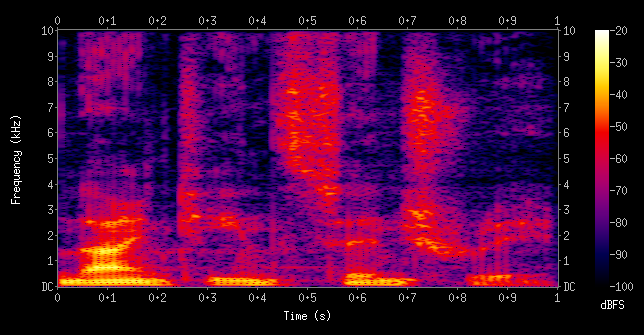
\includegraphics[width=12cm]{./Chapitre3/figures/spectrogramme.png}
  \caption{Représentation du signal en tant que spectogramme. La fréquence est modélisée en ordonnée et le temps en abscisse. L'énergie est visible grâce aux couleurs présentes: plus la couleur est chaude (rouge, orange, jaune) et plus l'énergie dégagée est importante. Image provenant de Wikipedia.}
  \label{fig:spectrogramme}
\end{figure}


Un spectrogramme est une représentation du signal audio mettant en avant l'intensité en fonction de la fréquence et du temps. %Comme on peut le voir sur la figure~\ref{fig:spectrogramme},
Il s'agit d'une représentation tridimensionnelle du signal audio. Cette transformation est possible en utilisant la transformation de Fourier qui permet de passer de l'espace temporel à l'espace fréquentiel. Les zones des énergies les plus fortes sont appellées des formants.

Cette représentation temps/fréquence peut être utilisée comme une image. Il est alors possible d'utiliser des systèmes de reconnaissance d'images afin de traiter des problématiques touchant au domaine de la parole~\cite{Stolar2017}.


\subsubsection{Coefficients Cepstraux en Fréquence Mel}
Les MFCCs, Mel-Frequency Cepstral Coefficients en anglais, sont des descripteurs spectraux utilisés très largement en traitement du signal audio, que ce soit en reconnaissance de la parole, en identification du locuteur ou en détection de concepts sémantiques par exemple. Ils sont issus d'un ensemble de traitements qui est appliqué sur le signal audio traditionnellement sur des fenêtres temporelles de 30 ms tous les 10 ms. Afin de modéliser l'évolution temporelle du signal, on utilise les dérivées premières et secondes de ces coefficients. Contrairement aux Linear Predictive Coding (LPC)~\cite{Rabiner1993},
%ou les Perceptual Linear Prediction (PLP)~\cite{Hermansky1990},
ces coefficients perceptifs sont adaptés à l'audition humaine puisqu'ils suivent l'échelle de perception de Mel. En effet, notre perception des sons n'est pas linéaire : nous percevons plus de différence entre des sons de 1000 et 2000 Hz qu'entre des sons de 7000 et 8000 Hz.

Robustes au bruit, ces coefficients permettent de représenter le spectre de façon compacte en éliminant les redondances entre les différents coefficients.

%Au total, nous avons donc une représentation en vecteurs de taille 39 pour chaque fenêtre de 10ms de signal, nous permettant de réduire considérablement le signal d'entrée, tout en gardant les informations essentielles contenues dans l'audio.

\subsubsection{Descripteurs prosodiques}
Dans le domaine du SER, il n'y a pas de consensus sur le meilleur ensemble de descripteurs à utiliser pour effectuer des tâches de reconnaissance d'émotions. C'est pour cela qu'il existe un grand nombre d'ensembles de descripteurs regroupant les différents indices acoustiques qui seront mis en relation avec les émotions. Ces indices sont soit extraits au niveau de fenêtres de courtes durées (30~ms le plus souvent), soit sur des fenêtres plus longues (plus d'une seconde) pour capturer des phénomènes para-linguistiques.

Traditionnellement, on prend un très grand nombre de descripteurs, comme par exemple l'ensemble de base extrait avec OpenSMILE~\cite{OPENSMILE}, qui compte 988 descripteurs acoustiques, puis on les filtre pour ne conserver que les plus pertinents par une sélection de descripteurs.

La sélection des descripteurs réduit la dimensionnalité de leur espace, supprime les données redondantes, non pertinentes ou bruitées. Elle apporte des effets bénéfiques directs aux systèmes : l'accélération du temps de traitement puisqu'il y a moins de données à traiter, l'amélioration de la qualité des données et donc de la performance des systèmes. De plus, elle peut permettre de rendre les résultats plus compréhensibles.
Cette sélection peut s'effectuer de plusieurs manières :
\begin{itemize}
    \item selon des méthodes de ranking, en comparant les descripteurs les uns aux autres.
    \item en utilisant des \textit{wrappers} : en utilisant le modèle de classification et en testant tous les descripteur les uns après les autres. Pour ce faire, on les enlève ou on les ajoute un à un et on sélectionne l'ensemble de descripteurs qui donne au modèle sa meilleure performance.
\end{itemize}
Néanmoins l'ordre de grandeur des corpus annotés en émotion peut vite poser problème si la dimension des descripteurs est trop importante.

Pour pallier ce problème, de plus petits ensembles de descripteurs, réalisés par des experts du domaine ont été proposés. On peut notamment citer l'ensemble INTERSPEECH 2009~\cite{Schuller2009} ainsi que \textit{The Geneva Minimalistic Acoustic Parameter Set} (GeMAPS) et sa version étendue (eGeMAPS)~\cite{Eyben2016}.

L'ensemble INTERSPEECH 2009 contient 384 descripteurs qui ont été utilisés comme référence lors du premier challenge en reconnaissance d'émotions en 2009. Il est composé de 16 descripteurs de bas niveau (Low Level Descriptors en anglais) :
\begin{itemize}
  \item \textit{zero crossing rate} : taux de passage par 0 du signal sur une fenêtre temporelle donnée.
  \item \textit{RMS energy} ou énergie moyenne quadratique : modélise la variation de l’énergie du signal à chaque fenêtre d'analyse.
  \item \textit{F0} ou fréquence fondamentale.
  \item \textit{Harmonic to noise ratio} ou rapport Harmonique-Bruit : modélise le bruit contenu dans le signal.
  \item \textit{MFCC} : les 12 premiers coefficients MFCCs sont utilisés.
\end{itemize}
Sur ces descripteurs sont calculées 12 fonctions statistiques (la moyenne, la variance, le coefficient de Pearson, de dissymétrie, le maximum, le minimum, la position relative, la plage de valeur et la régression linéaire). Soit, in fine, 16 descripteurs et leurs 16 dérivées sur lesquels on applique 12 fonctions pour un total de 384 descripteurs.

GeMAPS est composé de 18 descripteurs de bas niveau représentant des propriétés de fréquence, d’énergie, d’amplitude et des propriétés spectrales sur lesquels sont appliquées des fonctions statistiques pour un total de 62 descripteurs.
Nous reprenons la liste complète établie dans l'article de Eyben et al.~\cite{Eyben2016} dans le tableau~\ref{tab:egemaps}.

\begin{table}[h]
   \centering
   \begin{tabular}{| l |}
   \hline
       Paramètres fréquentiels \\
   \hline
       Hauteur de la voix (Pitch)  \\
       Tremblement de la voix (Jitter) \\
       Frequence des Formants 1,2,3 \\
       Bande passante (Bandwidth) des Formants 1,2,3 \\
   \hline
       Paramètres d'énergie et d'amplitude \\
   \hline
       Scintillement (Shimmer) \\
       Volume (Loudness) \\
       Ratio Harmonique-Bruit (Harmonics-to-Noise Ratio) \\
   \hline
       Paramètres spectraux \\
   \hline
       Ratio Alpha \\
       Index de Hammarberg \\
       2 pentes spectrales : 0-500Hz et 500-1500Hz \\
       Energie relative des Formants 1,2,3 \\
       Différence harmonique H1-H2 et H1-A3 \\
       MFCC 1 à 4 \\
       Flux spectral \\
   \hline
       Paramètres temporels  \\
   \hline
       Taux des pics de volume (Rate of loudness peaks) \\
       Moyenne et variance des zones parlées \\
       Moyenne et variance des zones non parlées \\
       Nombre de zones continues parlées par secondes \\
   \hline

   \end{tabular}
   \caption{Résumé des descripteurs de bas niveau (LLDs) utilisés dans l'ensemble eGeMAPS.}
   \label{tab:egemaps}
\end{table}


Comme la version courte de l’ensemble minimaliste ne contient aucun paramètre cepstral et très peu de paramètres dynamiques, on ajoute sept LLD (MFCCs, Flux spectral, Bande passante des formants 2,3) pour construire l'ensemble d'extension. En lui appliquant des fonctions statistiques, eGeMAPS contient un total de 88 descripteurs résumés dans le tableau~\ref{tab:egemaps}.
% résume toutes les caractéristiques retenues dans ces deux ensembles.

\subsubsection{Bag-of-Audio-Words (BoAW)}
Comme nous l'avons déjà indiqué, la sélection de la représentation de l'audio est un choix qui va directement influencer la qualité de la reconnaissance des émotions. C'est pour cela qu'il existe de nombreuses représentations, dont les sacs de mots-audio, ou BoAW. Inspiré des sacs de mots utilisés en NLP, il s'agit d'utiliser les LLDs sélectionnés pour former un lexique appelé \textit{codebook} de toutes les valeurs possibles, puis de les coder par un vecteur. Ce vecteur est alors utilisé en tant qu'entrée du système.

Cette solution présente comme avantage de renforcer la robustesse du système, vu que les LLDs en entrée sont en quelque sorte normalisées par ce processus. Ces features sont utilisées dans de nombreuses tâches reliées à la parole : la classification d'évènements sonores~\cite{Pancoast2012,Schmitt2016} ou la détection de plagiat~\cite{Liu2010} par exemple. Ils ont également été utilisés en reconnaissance d'émotions continues~\cite{Schmitt2016,Han2018}. %\textcolor{red}{Il manque une ref => codebook ?}.
%In this approach, feature vectors of acoustic LLDs are quantised according to a learnt codebook of audio words. Then, a histogram of the occurring ‘words’ is built.

\subsection{Descripteurs linguistiques}
Nous avons vu que lorsque l'on cherche à déterminer l'état émotionnel d'un locuteur à partir d'un enregistrement, l'approche la plus naturelle consiste à extraire des descripteurs acoustiques directement à partir du signal. On peut cependant ajouter des informations linguistiques, syntaxiques, phonémiques et sémantiques. Ces informations peuvent être extraites directement à partir d'une transcription automatique de la parole.

Les domaines du Sentiment Analysis et de l'Opinion Mining cherchent à identifier une opinion à partir d'un texte écrit. Il y a ici une différence sémantique significative entre opinion et état émotionnel, cependant les approches peuvent se rejoindre. On peut également considérer la transcription automatique comme un élément associé à la parole, et donc y retrouver des marqueurs de l'émotion. Nous détaillons dans cette partie certaines méthodes utilisées dans ces domaines pour transformer du texte (dans notre cas la transcription automatique) en descripteurs.

\subsubsection{Représentation en one-hot}
La représentation en \textit{one-hot}, comme illustrée sur la figure~\ref{fig:onehot}, correspond à associer à chaque mot un vecteur de binaires d'une taille fixe. On rassemble tous les mots-types (appelés token en anglais) utilisés dans ce que l'on nomme un vocabulaire. Puis pour chaque mot-type de ce vocabulaire, on associe un vecteur binaire unique. Cette méthode présente l'avantage d'être exhaustive et facile à mettre en œuvre, cependant la représentation est très volumineuse : le vecteur sera de la taille du vocabulaire et elle contiendra principalement des zéros.

\begin{figure}[h]
  \centering
  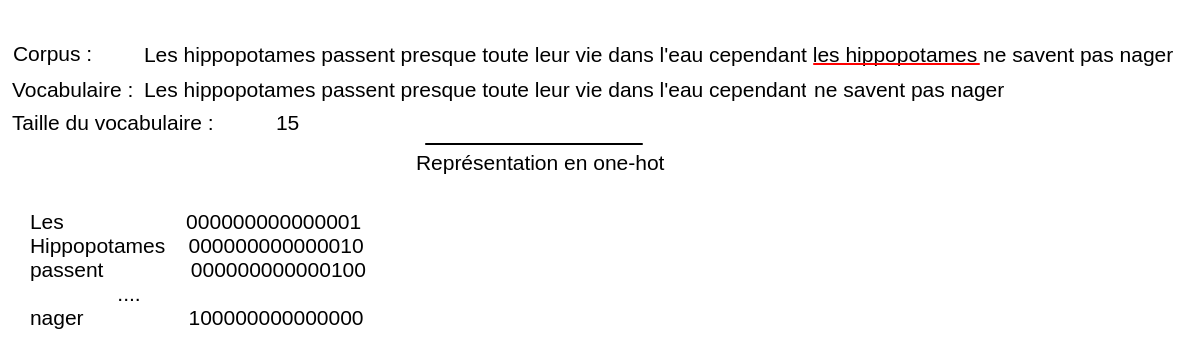
\includegraphics[width=15cm]{./Chapitre3/figures/onehot.png}
  \caption{Transformation d'un corpus en représentation one-hot.}
  \label{fig:onehot}
\end{figure}


Cette représentation permet de réaliser des opérations numériques directement sur les vecteurs \textit{one-hot}. Cependant elle ne porte aucune information sur le contexte (la position du mot-type dans la séquence), la sémantique ou sur le nombre d’occurrence de chaque mot-type.

\subsubsection{Représentation statistique}
Parmi les représentations statistiques des données textuelles, les plus courantes et les plus mises en place sont les méthodes TF (Term Frequency) et TF-IDF (Term Frequency-Inverse Document Frequency) qui prennent en compte la distribution des tokens dans les documents.
Le TF est défini comme ``the frequency of occurrence of the terms in the document or query texts''~\cite{salton_tf_idf}.
C'est-à-dire que le TF d'un mot-type $t$ présent dans un document $d$ correspond au nombre d’occurrences de $t$ dans $d$ divisé par le nombre total de tokens dans le document (Eq.~\ref{eq:tf}).
\begin{equation}
    \text{TF}(d,t) = \dfrac{\text{Nombre de } t \text{ dans } d}{\text{Nombre de tokens dans } d}
\label{eq:tf}
\end{equation}


Toujours selon Salton~\cite{salton_tf_idf}, le facteur IDF varie ``inversely with the number of documents $n$ to which a term is assigned in a collection of $N $documents. A typical idf factor may be computed as log $N/n$''.
Le facteur IDF correspond à l'inverse du rapport entre le nombre de documents où le token $t$ apparait sur le nombre total de documents $N$ (Eq.~\ref{eq:idf}).

\begin{equation}
    \text{IDF(t)} = - log\left(\dfrac{N}{\text{Nombre de documents où } t \text{ est présent} + 1} \right)
\label{eq:idf}
\end{equation}

Le TF-IDF est alors défini comme le produit des deux termes précédents comme indiqué dans l'équation~\ref{eq:tfidf}.
%Le +1 au dénominate
Pour permet d'éviter les cas où aucun document ne contiendrait le token $t$ et donc la division par zéro. Cette approche permet que les tokens qui sont soit trop fréquents, soit présents dans tous les documents, soient moins mis en avant par la représentation.

\begin{equation}
    \text{TF-IDF}(t,d) = \text{TF}(t,d) \times \text{IDF}(t)
\label{eq:tfidf}
\end{equation}

Ces méthodes statistiques ont fait leurs preuves~\cite{Martineau2009,Cambria2013,Pimpalkar2020}, même si on leur préfère maintenant des méthodes qui intègrent des aspects sémantiques notamment.

\subsubsection{Plongement de mots}
\begin{figure}[h]
  \centering
  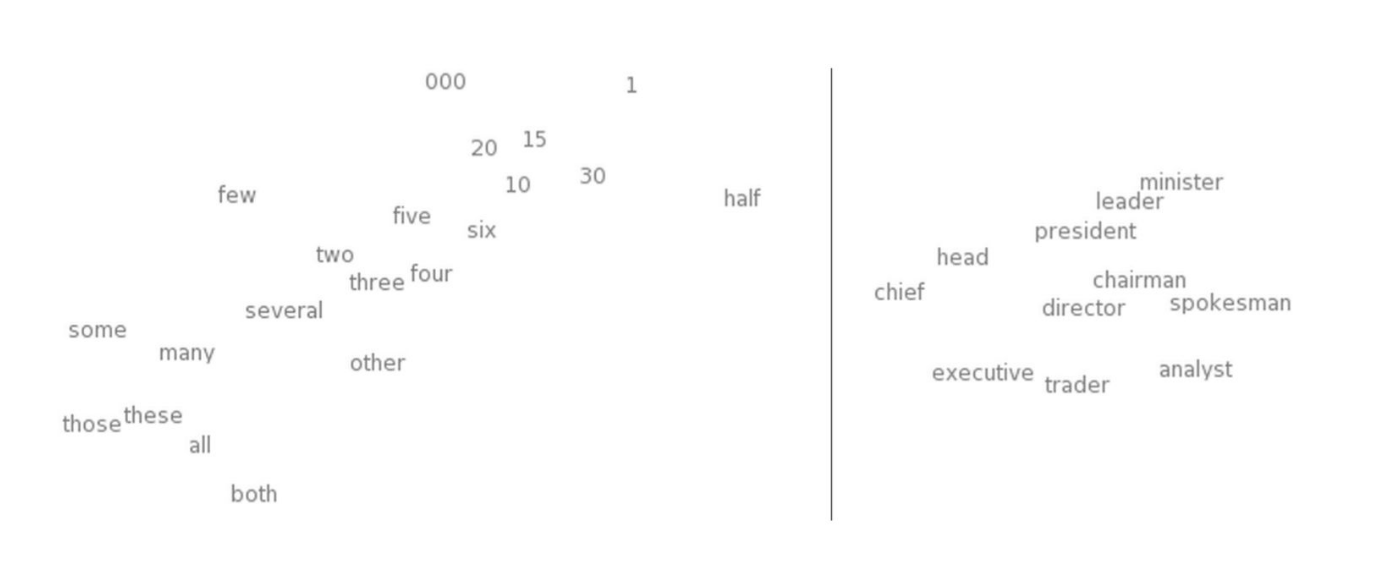
\includegraphics[width=14cm]{./Chapitre3/figures/word2vec.png}
  \caption{Représentation de plongements de mots en deux dimensions. Les mots de gauche correspondent au regroupement des termes associés au numérique. Les mots de droite correspondent aux termes associés à l'emploi. Issue des travaux de Turian et al.~\cite{Turian2010}.}
  \label{fig:word2vec}
\end{figure}


Les plongements de mots (word embeddings en anglais) ont été présentés par Bengio et al.~\cite{Bengio2003}.
A l'origine, un modèle neuronal est appris pour une tâche de reconnaissance automatique de la parole sur un grande nombre de données. Une fois le modèle entrainé, on peut prendre le réseau dans l'autre sens et supprimer les couches basses (proches de l'audio) et figer les poids afin de créer un extracteur capable de calculer des embeddings, c'est-à-dire les représentations internes du réseau de neurones, à partir d'une entrée textuelle. Ces embeddings permettent d'avoir accès à une nouvelle représentation des mots dans un espace dense et à valeurs réelles.
On projette les mots dans un espace de faible dimension, tout en isolant ensemble les mots qui ont des similarités sémantiques et syntaxiques~\cite{Ghannay2017}. Cela permet d'associer à chaque token un vecteur de valeurs réelles, de dimension bien inférieure à celle utilisée pour la représentation \textit{one-hot}. Chaque vecteur est ensuite inscrit dans un dictionnaire, et on peut alors remplacer chaque mot par le vecteur le représentant.

Leur utilisation et leur pertinence a été démontré dans de nombreuses tâches, notamment des tâches de TALN: l’étiquetage morphosyntaxique, la reconnaissance d’entités nommées, la détection de mention~\cite{Turian2010,Bansal2014} et de compréhension de la parole~\cite{Mesnil2013,Yao2014,Liu2016}.

Parmi les plongements lexicaux les plus utilisées, on trouve Word2vec~\cite{word2vec} et GloVe~\cite{Pennington2014}.
Plus précisément, les plongements de Word2Vec sont appris soit avec un algorithme de sac de mots continus (continuous bag of words, CBOW) qui prédit un mot sachant son contexte lexical, soit l'algorithme Skip-gram qui prédit les mots du contexte sachant le mot d'entrée.

Il est utile de noter que ce genre de représentation peut être visualisée dans un espace plus restreint, typiquement en deux dimensions en utilisant une réduction de dimensions (par exemple une Analyse en Composantes Principales). Ainsi les expérimentateurs peuvent observer les rapprochements sémantiques ou syntaxiques détectés par le système, comme l'illustre la figure~\ref{fig:word2vec}.

\section{Évaluation des performances}
De nombreuses métriques ont été utilisées au fur et à mesure de l'avancée du domaine pour évaluer les performances des systèmes de reconnaissance d'émotions dans la parole suivant le type de tâche : classification ou régression.

Pour les tâches de classification les métriques d'\textit{accuracy}, de précision et de rappel pondérés ou non pondérés sont les métriques les plus utilisées traditionnellement. On peut notamment se référer aux challenges INTERSPEECH en émotions de 2009 et 2011~\cite{Schuller2009,Schuller2011} qui utilisent le rappel moyen non pondéré comme métrique afin de compenser le biais de données souvent très déséquilibrées en nombre d'instances par classe.

En ce qui concerne les tâches de régression, l'erreur quadratique moyenne est une métrique efficace qui a été largement utilisée avant que des campagnes d'évaluation~\cite{AVEC2017} ne standardisent l'utilisation du Coefficient de Corrélation de Concordance (CCC) comme la mesure de référence pour l'évaluation de systèmes de reconnaissance de l'émotion continue.

\subsection{Tâche de classification}

\subsubsection{Matrice de confusion et scores associés}
La matrice de confusion est une matrice permettant de mesurer la performance d'un système de classification. Elle permet d'associer pour chaque classe de référence, les classes prédites par le système.
À chaque segment émotionnel est associée une classe qui définit l'état émotionnel de référence de la personne. Cette matrice est donc mise en place en tant qu'évaluation lorsque les émotions sont de nature discrètes. Grâce à elle, on peut retrouver les différentes erreurs du système et les quantifier. Un exemple de matrice de confusion est donné par le tableau~\ref{tab:matriceConf}. Les lignes correspondent aux références, et les colonnes aux prédictions d'un système.

\begin{table}[h]
  \centering
\begin{tabular}{|l|l|c|c|c|c||c|c|}
\cline{3-6}
\multicolumn{1}{c}{}       &         &\multicolumn{4}{c||}{\textbf{Prédiction}} \\ \cline{4-8}
\multicolumn{1}{c}{}       &             & joie        & neutre      & colère &total      &précision &rappel\\ \hline
\multirow{3}{*}{\rotatebox[origin=c]{90}{\textbf{Réf}}} &joie   & \textbf{90} & 11          & 2 &103                &0.900 &0.874\\ \cline{2-7}
                     & neutre & 4           & \textbf{80} & 10       &94        &0.889 &0.851 \\ \cline{2-8}
                     & colère & 6           & 9           & \textbf{20} &35      &0.625 &0.571 \\ \cline{2-8} \cline{2-8}
                     %& total  & 100         & 90          & 32           & & \\ \hline
\end{tabular}
\caption{Matrice de Confusion entre trois classes émotionnelles : la joie, le neutre et la colère. Les colonnes correspondent aux prédictions du système et les lignes correspondent aux références. On voit que sur 100 prédictions de la classe joie, seules 90 sont pertinentes et le système a mal prédit 13 segments qui ne devraient pas être dans la classe joie.}
\label{tab:matriceConf}
\end{table}

%\begin{figure}[h]
  \centering
  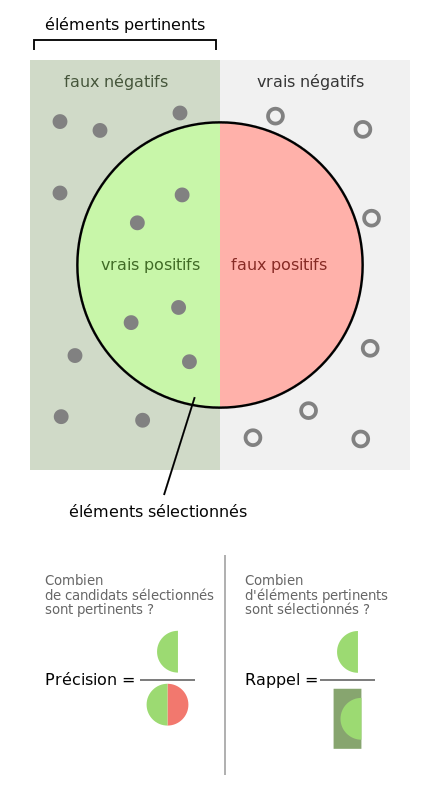
\includegraphics[width=7cm]{./Chapitre3/figures/precisionRappel.png}
  \caption{Représentation schématique de la précision et du rappel. Image provenant de Wikipedia}
  \label{fig:precisionRappel}
\end{figure}


Cette présentation permet notamment de visualiser si une classe est mieux prédite que d'autres. Il est facile de relever si le système est performant en se basant sur la diagonale, qui regroupe les vrais positifs et donc de calculer l'\textit{accuracy} définie par le nombre de segments correctement prédits sur le nombre total de segments $N$ (eq.~\ref{eq:accuracy}), tandis que les autres cases correspondent à des erreurs du système.

\begin{equation}
\text{Ac} = \dfrac{\text{Nb de prédictions vraies}}{N}
\end{equation}\label{eq:accuracy}

Cette matrice de confusion permet également de calculer le rappel et la précision de chaque classe. La précision $P_i$ de la classe $c_i$, correspond au nombre de segments de la classe $c_i$ correctement prédits parmi tous les segments prédits comme étant de classe $c_i$. (eq.~\ref{eq:precision}). Le rappel $R_i$ de la classe $c_i$ est donné par l'équation~\ref{eq:rappel} et correspond au nombre de segments correctement prédits parmi tous les segments de la classe $c_i$

\begin{equation}
  P_i = \frac{\text{nb predictions vraies}_i}{\text{nb predictions vraies}_i + \text{nb predictions fausses}_i}
  \label{eq:precision}
\end{equation}

\begin{equation}
  R_i = \frac{\text{nb predictions vraies}_i}{\text{nb segments de classe } c_i}
  \label{eq:rappel}
\end{equation}

Bien que pratique, la matrice de confusion ne permet pas de donner un score unique pour le système.


\subsubsection{Précision ou rappel pondéré et non-pondéré}

Afin d'avoir un score global de la classification des émotions, on peut moyenner les précisions et rappels par classe en pondérant ou non en fonction du nombre de segments par classe. La précision moyenne non pondérée (unweighted average precision, UAP) est obtenu en prenant simplement la moyenne des précisions par classe.
La précision moyenne pondérée (weighted average precision, WAP) est calculée en prenant la moyenne des précisions par classe suivant l'équation~\ref{eq:WA} où $N$ est le nombre de segments total et $n_i$ le nombre de segments dans la classe $c_i$. Pour éviter des possibles confusions entre les métriques de précision et de rappel, comme dans les travaux de Lee et Tashev~\cite{Lee2015} ou de Han et al.~\cite{Han2014} (où la définition de l'\textit{accuracy} par classe est ambigüe) nous indiquerons systématiquement sur quelle métrique s'applique la pondération.


\begin{equation}
  \text{WAP} = \dfrac{1}{N}\sum^n_{i=1}n_i \cdot P_i
  \label{eq:WA}
\end{equation}

La mesure de précision moyenne pondérée permet de calculer la performance d'un système de reconnaissance, mais elle ne rend pas bien compte des différences de performance entre les classes. Notamment si le corpus est déséquilibré et que le système a tendance a favoriser la classe majoritaire, on aura toujours des taux de WAP importants. Dans l'exemple du tableau~\ref{tab:matriceConf}, la classe colère n'est pas bien reconnue. Pourtant si on calcule la UAP ($\frac{0.9+0.851+0.571}{3}$) on trouve $0,774$ soit une performance élevée de $77,4\%$ de bonne prédiction. Or les prédictions de la classe colère ont une précision de $57,1\%$. L'utilisation d'une moyenne non pondérée permet de mettre en évidence ce phénomène et d'apporter une métrique plus équitable entre les différentes classes.

Nous pouvons également utiliser le rappel moyen non-pondéré, comme lors des challenges INTERSPEECH~\cite{Schuller2009,Schuller2011}. Il est calculé selon l'équation~\ref{eq:UAR} et permet de déterminer combien d'éléments pertinents ont été retrouvés.

\begin{equation}
  UAR = \dfrac{1}{n} \sum_{i=1}^n R_i
  \label{eq:UAR}
\end{equation}

\subsubsection{F-mesure}

La F-mesure, ou F-score en anglais, combine à la fois la précision et le rappel selon l'équation~\ref{eq:Fmesure}. Elle est comprise entre 0 et 1. Plus elle est grande, plus le système évalué est performant. Elle peut être calculée par classe sur les précisions $P_i$ et rappels $R_i$.

\begin{equation}
  F = 2 \left( \frac{precision.rappel}{precision+rappel} \right)
  \label{eq:Fmesure}
\end{equation}

Néanmoins toutes les reconnaissances d'émotions ne se font pas sur des émotions discrètes, il existe donc d'autres indicateurs utilisés pour mesurer la performance des systèmes.

\subsection{Tâche de régression}

\subsubsection{Erreur quadratique moyenne}
L'erreur quadratique moyenne est une métrique qui est utilisée dans l'évaluation des systèmes de reconnaissance d'émotions continues~\cite{AVEC2017}. Elle permet de calculer un score d'accord entre deux séries temporelles, ici les annotations de références et les prédictions du système. Afin que cette métrique soit de la même dimension que les valeurs de référence, on utilise principalement la racine de l'erreur quadratique moyenne, RMSE pour \textit{Root Mean Square Error}. Cette métrique se calcule selon l'équation~\ref{eq:RMSE_score} entre les valeurs prédites $x_i$  et les valeurs de références $y_i$. $n$ correspond au nombre de valeurs de la série temporelle.

\begin{equation}
    RMSE = \sqrt{\frac{1}{n}\Sigma_{i=1}^{n}{\Big(y_i - x_i\Big)^2}}
\label{eq:RMSE_score}
\end{equation}

Elle est généralement comprise entre 0 et 1 (en fonction des valeurs $x_i$ et $y_i$). Comme il s'agit d'une mesure d'erreur, les systèmes à haute performance se rapprochent de 0, ce qui indique un ajustement parfait entre les références et les prédictions. Cette métrique n'est pas exempte d'inconvénients. En effet, elle est très sensible aux valeurs extrêmes et elle est difficilement comparable à d'autre scores calculés sur des valeurs d'ordres de grandeur différents.

\subsubsection{Coefficient de Corrélation de Concordance}
Le coefficient de corrélation de concordance (CCC)~\cite{CCC} a été établi comme un standard d'évaluation lors notamment des trois précédents Audio/Visual Emotion Challenge and Workshops (AVEC)~\cite{AVEC2017,AVEC2018,AVEC2019}. Cette métrique évalue l'accord entre deux séries temporelles selon l'équation~\ref{eq:CCC_score}, où $x$ et $y$ sont les deux séries temporelles, dans notre cas la prédiction et la référence. $\mu_x$, $\mu_y$ correspondent à leur moyenne, $\sigma_x$, $\sigma_y$ à leur écart-type et $\rho$ le coefficient de corrélation entre ces deux variables aléatoires.

 \begin{equation}
    CCC = \frac{2\rho\sigma_x\sigma_y}{\sigma_x^2 + \sigma_y^2 + (\mu_x - \mu_y)^2 + \epsilon}
 \label{eq:CCC_score}
 \end{equation}

Plus le CCC s'approche de 1 et plus le système est considéré comme performant. A l'inverse, plus le score s'approche de 0 et moins il y a de corrélation entre les prédictions et les références, dénotant un système peu performant.
Cette métrique n'est pas définie dans le cas où les deux séries temporelles $x$ et $y$ sont constantes et de mêmes moyennes. On ajoute un $\epsilon$ au dénominateur pour pallier à ce problème lors de l'implémentation.

Cette métrique sera utilisée dans les travaux de cette thèse pour évaluer la performance des systèmes de prédiction continue de la satisfaction. %Afin de nuancer les différences de scores entre différentes configurations de nos systèmes, nous avons mis en place un intervalle de confiance, qui est explicité dans le chapitre~\ref{chapitre6}.

\section{Fusion de modalités}
Afin de pouvoir profiter à la fois des informations acoustiques et linguistiques, il est pertinent de fusionner ces deux modalités pour avoir un système performant et plus robuste~\cite{Wollmer2013,Alam2014,Atrey2010,Liu2018}. La fusion de modalités est assez vaste: il est possible également d'inclure des informations issues de vidéos ou de capteurs physiologiques, dont nous avons parlé au premier chapitre.

Dans le cadre de cette thèse, nous sommes principalement intéressés par les modalités acoustiques et linguistiques, puisque les autres des modalités ne peuvent pas être récupérées depuis les centres d'appels.
\\
\\
\textbf{Type de fusion}

La fusion peut s'effectuer de différentes manières.
\begin{itemize}
  \item Fusion des features~\cite{Wollmer2013,Alam2014,Atrey2010} : La fusion s'opère au niveau des features, on concatène les vecteurs représentant les différentes modalités. Cette méthode augmente le nombre de features en entrée du système et peut donner des résultats très différents en fonction de la stratégie de normalisation des données. En effet, il peut être compliqué pour le système de comprendre que les données représentent deux espaces différents. Donc il est courant de normaliser les données afin de se référer à un seul espace.
  \item Fusion des modèles~\cite{Atrey2010,Liu2018} : Plusieurs apprentissages sont faits de façon distincts pour chaque modalité jusqu'à une certaine couche dans le réseau de neurones. Les couches sont alors fusionnées, et l'apprentissage reprend. Plus la fusion arrive tôt et plus le système doit en théorie avoir un bon pouvoir de généralisation.
  \item Fusion de décision~\cite{Wollmer2013,Atrey2010} : Plusieurs apprentissages sont faits de façon distincts pour chaque modalité. On prend la prédiction de chacun des modèles et on les fusionne. S'il s'agit d'une classification, on peut fusionner par vote majoritaire par exemple. S'il s'agit d'une régression, on peut faire la moyenne des sorties. De plus, on peut facilement mettre plus d'importance sur une des modalités en faisant une moyenne pondérée des sorties.
\end{itemize}

\section{Notre référence : AVEC}

\begin{table}[]
    \centering
    \begin{tabular}{| l | l | l | c | c | c |}
        \hline
        \textbf{Models} &\textbf{Modalité} &\textbf{Features} &\multicolumn{3}{c|}{\textbf{SEWA}} \\ \cline{3-6}
        & & &activation &valence &liking \\
        \hline
        \multicolumn{6}{|l|}{AVEC 2017~\cite{AVEC2017} : Sur les conversations allemandes} \\
        \hline
        SVR      &audio &BoAW~\cite{Schmitt2016} &.344  &.351 &.081 \\
        SVR      &audio &BoTW                    &.373  &.390 &.314 \\
       \hline
       \multicolumn{6}{|l|}{Huang et al.~\cite{Huang2017} : Sur les conversations allemandes} \\
       \hline
       LSTM     &audio &eGeMAPS-88  &.506  &.455 &.193 \\
       LSTM     &audio &IS10        &.465  &.440 &.227 \\
       LSTM     &audio &Bottle-neck~\cite{Fer2015} &.533  &.466 &     \\
       LSTM     &audio &Mfcc        &.341  &.421 &     \\
       LSTM     &texte &BoTW        &.451  &.518 &.473 \\
        \hline
        \multicolumn{6}{|l|}{AVEC 2018~\cite{AVEC2018} : Sur les conversations allemandes} \\
        \hline
        biLSTM-2 &audio &eGeMAPS-88  &.124  &.112 &.001 \\
        biLSTM-2 &audio &Mfcc        &.253  &.217 &.136 \\
         \hline
       \multicolumn{6}{|l|}{Huang et al.~\cite{Huang2018} : Sur les conversations allemandes} \\
       \hline
       LSTM     &audio &eGeMAPS-88   &.497  &.438 &.281 \\
       LSTM     &audio &eGeMAPS-89   &.520  &.461 &\textbf{.335} \\
       LSTM     &audio &eGeMAPS-176  &.514  &.493 &.217 \\
       LSTM       &texte &Word2Vec-300   &\textbf{.597}  &\textbf{.600} &.454 \\
       LSTM-2     &texte &BoW            &  & &.407 \\
       LSTM-2     &texte &Word2Vec       &  & &\textbf{.480} \\
       LSTM-2     &texte &GloVe          &  & &.413 \\
        \hline
        \multicolumn{6}{|l|}{AVEC 2019~\cite{AVEC2019} : Sur les conversations allemandes et hongroises} \\
        \hline
        biLSTM-2 &audio &eGeMAPS-88  &.371 &.286 &.159 \\
        biLSTM-2 &audio &Mfcc        &.326 &.187 &.144 \\
         \hline
       \multicolumn{6}{|l|}{Schmitt et al.~\cite{Schmitt2019} : Sur les conversations allemandes} \\
       \hline
       \rowcolor{Red}
       CNN      &audio &eGeMAPS-47    &\textbf{.571}  &.517 & \\
       \rowcolor{Red}
       biLSTM-4 &audio &eGeMAPS-47    &.568  &\textbf{.561} & \\
       \hline
    \end{tabular}
    \caption{Compilation des scores de CCC sur l'ensemble de développement de SEWA sur les 3 dimensions : activation, valence et \textit{liking}. L'acronyme BoAW signifie \textit{Bag-of-audio-words}, BoTW signifie \textit{Bag-of-text-words}, SVR signifie Support Vector Regression~\cite{Smola2004}, proche des SVM mais applicable à des problèmes de régression et donc à une annotation continue. Les différents nombres associés aux features de type eGeMAPS dénotent de différentes configurations utilisées autour de ces sets : soit avec une sélection reduite des LLDs (47), soit avec l'ajout d'information sur le locuteur courant (89 et 176).}
    \label{tab:avec}
\end{table}

Si nous nous replaçons dans le contexte de la thèse, nous cherchons à construire et donc à évaluer un système de reconnaissance des émotions continues depuis la parole. Dans ce cadre, nous avons recherché dans la littérature, des systèmes et des expérimentations qui soient comparables à nos recherches. Nous avons choisi de nous référer aux campagnes AVEC, \textit{Audio/Visual Emotion Challenge and Workshop}.

Ce challenge, qui en était à sa huitième itération en 2018, vise à comparer les méthodes de traitement multimédia et d'apprentissage automatique pour l'analyse automatique de la santé et des émotions dans les modalités audio et visuelles. Ces campagnes sont divisées en différents objectifs qui gravitent autour des émotions: de la détection de dépression, de bipolarité, d'état d'esprit ou d'émotions issues de différentes cultures par exemple. Comme ces campagnes s'appuient sur des corpus multimodaux comme RECOLA~\cite{Ringeval2013} et SEWA~\cite{SEWA} notamment, les émotions peuvent être détectées à partir de différentes modalités, notamment depuis la parole et les expressions faciales.

Afin de pouvoir nous comparer à l'état de l'art, nous avons décidé de comparer nos résultats à ceux obtenus sur le corpus SEWA, dont nous avons parlé dans ce chapitre.
Ce corpus considère trois dimensions émotionnelles : la valence, l'activation et le \textit{liking} qui correspond à l'appréciation par les participants des clips visionnés en amont. Il est utilisé notamment dans les campagnes AVEC depuis 2017~\cite{AVEC2017,AVEC2018,AVEC2019} et sert actuellement de baseline dans la communauté. Nous nous intéressons donc à la tâche de régression audio uniquement.

Nous résumons dans le tableau~\ref{tab:avec}, différents résultats obtenus qui utilisent la partie Allemande et Hongroise du corpus, soit celle à laquelle nous avons accès. Comme nous pouvons le voir, de nombreux ensembles de features et types d'algorithme ont été utilisés pour la reconnaissance des émotions depuis la parole pour le corpus SEWA.
Pour ce qui est de la modalité acoustique, nous pouvons voir que les systèmes les plus performants ont des scores de 0.571 pour l'activation, 0.561 pour la valence et 0.335 pour le liking. Nous voyons que la plupart des participants ont utilisé des systèmes CNN ou LSTM (détaillés dans le chapitre~\ref{chapitre5}) pour résoudre la régression. En regardant les deux études de Huang et al.~\cite{Huang2017,Huang2018}, nous pouvons remarquer que le choix de l'ensemble de descripteurs influence fortement sur les scores des systèmes de regression. On remarque également une prédominance de l'utilisation des eGeMAPS, qui donne les meilleurs scores.

Pour ce qui est de la modalité linguistique, on peut notamment remarquer que l'on retrouve principalement l'utilisation de plongements de mots (word2vec et GloVe) et le même type d'architecture que pour la modalité acoustique, avec une variation du réseau LSTM, qui possède deux couches pour les expérimentations sur le liking.

Si on compare les résultats à ceux trouvés par la modalité acoustique, les scores maximum sont assez similaires : 0.597 contre 0.571 pour l'activation, 0.600 contre 0.561 pour la valence. On observe également une nette amélioration pour le liking : 0.480 au lieu de 0.335. En général, on trouve des scores un peu plus élevés en utilisant la modalité linguistique~\cite{Gunes2013}. Cela peut être dû au fait que les descripteurs utilisés sont plus adaptés ou que les architectures neuronales sont plus adaptées à ce type de données.

Dans le cadre de cette thèse, nous cherchons à mettre en place des solutions neuronales profondes. Nous avons donc fait le choix de nous comparer aux résultats obtenus par Schmitt et al.~\cite{Schmitt2019} correspondant aux lignes rouges du tableau.
%\begin{table}[]
    \centering
    \begin{tabular}{| l | l | c | c | c |}
        \hline
        \textbf{Models} &\textbf{Features} &\multicolumn{3}{c|}{\textbf{SEWA}} \\ \cline{3-5}
        & &activation &valence &liking \\
        \hline
        \multicolumn{5}{|l|}{AVEC 2017~\cite{AVEC2017} : Sur les conversations allemandes} \\
        \hline
        SVR      &BoTW       &.373  &.390 &.314 \\
       \hline
       \multicolumn{5}{|l|}{Huang et al.~\cite{Huang2017} : Sur les conversations allemandes} \\
       \hline
       LSTM     &BoTW        &.451  &.518 &.473 \\
        \hline
       \multicolumn{5}{|l|}{Huang et al.~\cite{Huang2018} : Sur les conversations allemandes} \\
       \hline
       LSTM       &Word2Vec-300   &\textbf{.597}  &\textbf{.600} &.454 \\
       LSTM-2     &BoW            &  & &.407 \\
       LSTM-2     &Word2Vec       &  & &\textbf{.480} \\
       LSTM-2     &GloVe          &  & &.413 \\
       \hline
    \end{tabular}
    \caption{Compilation des scores de CCC sur l'ensemble de développement de SEWA sur les 3 dimensions : activation, valence et \textit{liking}. L'accronyme BoTW signifie \textit{Bag-of-text-words}, SVR signifie Support Vector Regression~\cite{Smola2004}, proche des SVM mais applicable à des problèmes de régression et donc à une annotation continue.}
    \label{tab:avectexte}
\end{table}


% \section{Sentiment Analysis et Opinion Mining}
% Utiliser le texte pour déterminer l'état émotionnel est une voie de plus en plus empruntée grâce, notamment, à la performance des systèmes de reconnaissance de la parole actuels.
% Des domaines tels que l'Analyse de Sentiments et la Détection d'Opinion, utilise des données textuelles de type livres, témoignages ou plus récemment des tweets et  des contenus en ligne afin d'extraire des informations. On peut également considérer la transcription automatique comme un élément associé à la parole, et donc y retrouver des marqueurs de l'émotion.
%
% Dans ces domaines, on cherche alors l'émotion dans l'aspect sémantique de la phrase, dans les diffluences ou les répétitions.
%
% Le terme \textit{Détection d'Opinion} (traduction de Opinion Mining) a été popularisé par les travaux de Kushal Dave~\cite{Dave2003}, définissant le domaine comme traitant un ensemble de données pour en retirer ses qualités et ses caractéristiques afin de statuer sur l'avis du sujet~\cite{Pang2008}. Le domaine \textit{Analyse de Sentiments} (traduction de Affect Analysis) a pris de l'ampleur depuis les travaux de Sanjiv Das, Mike Chen et Richard Tong au début du XXIe siècle~\cite{Das2007,Tong2001}. Il diffère de l'Opinion Mining : la majorité de ces travaux se concentrent sur la classification des avis ou de phrases en polarité (positif ou négatif). Mais ces domaines de recherche restent très fortement liés et constituent la plus grande partie de recherche d'indices émotionnelles à base de données textuelles.
%
% Des outils tel que des dictionnaires de polarité, FAN~\cite{Monnier2014} par exemple, permettent de colorer émotionnellement des mots ou des phrases, ou encore des analyseurs de syntaxe tel que Macaon~\cite{Nasr2011} permettent d'étudier la structure d'un énoncé pour faire ressortir sa forme morphosyntaxique. Ces outils sont utilisés dans la reconnaissance d'émotions que ce soit à l'échelle d'un segment de parole, d'une phrase ou d'un document.
%
% \subsection{Corpus existant}
% De nombreux corpus de texte existent, mais peu sont annotés en émotion. Si nous nous référons aux campagnes AVEC, la transcription automatique de la parole est utilisée en tant que donnée textuelle. Cette transcription est ensuite alignée aux annotations, permettant d'obtenir ainsi des données annotées.
%
% Il est également possible de constituer son propre corpus en confrontant un texte à des lexiques d'émotions comme par exemple le lexique NRC~\cite{Mohammad2013} disponible dans 105 langues, SentiWordNet~\cite{Sebastiani2006} ou encore le lexique FAN~\cite{Monnier2014}.
% Le lexique NRC contient 14 182 mots et sont associés à 10 catégories différentes (anticipation, colère, tristesse, joie, peur, confiance, dégoût, surprise, positive, négative). Chaque mot peut être associé à plusieurs catégories ou à aucune.
% Le dictionnaire French Affective Norms (FAN) propose quant à lui, un score de valence (entre 0 et 10) pour plus de 1000 mots, annotés par plus de 400 participants.
%
% Il est également possible de se tourner vers des corpus déjà construits, comme ceux utilisés lors des campagnes SemEval. Par exemple des titres d'article provenant de journaux~\cite{Strapparava2010} ou encore un corpus constitué de livres pour enfants~\cite{Etienne2020}. Les données de SemEval sont annotés en catégories discrètes (colère, dégoût, peur, joie, tristesse, surprise et valence) par une échelle allant de 0 à 100 pour chaque émotion. 0 signifiant l'absence de l'émotion dans le titre et 100 la charge émotionnelle maximale. La valence varie entre -100 (négative) et 100 (positive) avec 0 (neutre) au milieu. Le corpus de livres pour enfants est annoté en 10 catégories discrètes (colère, dégoût, joie, peur, surprise, tristesse,culpabilité, embarras, fierté et jalousie). Cette annotation est enrichie en plusieurs concepts, notamment le mode d'expression de l'émotion : désignée, comportementale, montrée, étayée.
%
% De nombreux autres corpus existent afin de traiter un maximum de tâches en lien avec les émotions. Mais ces corpus sont difficilement utilisables en l'état, il est important de les transformer afin de les rendre compréhensibles par les systèmes d'apprentissage.

% \subsection{Les scores de systèmes à l'état de l'art tirés d'AVEC}
%
% \begin{table}[]
    \centering
    \begin{tabular}{| l | l | c | c | c |}
        \hline

       \hline
    \end{tabular}
    \caption{J'ai pas retrouvé de scores pour la fusion acoustiques et linguistiques. On a toujours de la vidéo dedans.}
    \label{tab:avecmulti}
\end{table}

%
% Une fois encore, nous nous intéressons aux scores présentés lors du challenge AVEC. La multi-modalité étant un aspect prédominant dans cette campagne, les données comportent également des vidéos qui peuvent être utilisés par les participants. Dans le tableau~\ref{tab:avecmulti}, nous ne rapportons que les scores des modalités acoustiques et linguistiques.

\section{Conclusion}
Dans ce chapitre, nous avons résumé les principaux composants de la reconnaissance des émotions depuis la parole, sans oublier la reconnaissance depuis le texte. A partir de ces connaissances, nous avons pu établir un référentiel sur la tâche que nous cherchons à accomplir. En effet, nous avons fait le choix de nous comparer au corpus SEWA et aux différents systèmes et features utilisés avec celui-ci. De plus, nous avons introduit le principe de fusion des modalités, qui apparaîtra dans les contributions de cette thèse.

Dans la prochaine partie, nous allons nous concentrer sur les contributions de cette thèse : de la construction d'un corpus répondant à nos besoins, à la mise en place de systèmes de reconnaissance des émotions performants et l'analyse des résultats obtenus.


\part{Contributions}

\clearemptydoublepage
\chapter{Construction du corpus AlloSat}
\label{chapitre4}
"Vos clients les plus mécontents sont votre meilleure source d’apprentissage" (Bill Gates)

\section{Motivation}
L'un des objectifs de cette thèse est de comprendre et de reconnaître l'état émotionnel de clients étant en relation téléphonique avec des agents de centre d'appels. L'objectif de ces conversations sont en général soit d'acheter un produit (service d'abonnement, service d'achat), soit de régler un problème (plainte, service après vente, service de réclamation), soit de demander des informations diverses sur une entreprise ou leur produit. Selon l'exigence industrielle, deux émotions sont primordiales dans la relation clientèle : la satisfaction, facteur de fidélité et de diffusion de la marque ainsi que la frustration, facteur d'attrition du client et de "mauvaise publicité". Ces deux émotions, comme nous avons pu le voir dans le chapitre~\ref{chapitre1}, peuvent s'inscrire dans différentes théories discrètes ou continues.
Nous avons choisi de les inscrire dans un espace continu, en créant la dimension de satisfaction comme explicité dans la figure~\ref{fig:satisfactionAxis}. En effet, outre l'émotion brute, la variation de son intensité et de sa durée sont des indicateurs cruciaux pour améliorer l'expérience du client.

\begin{figure}[h]
  \centering
  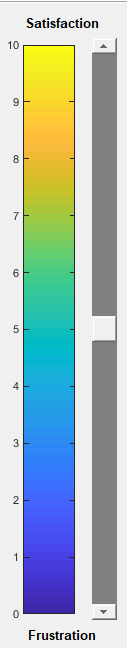
\includegraphics[width=\textwidth]{./Chapitre4/figures/satisfactionAxis.png}
  \caption{L'axe de satisfaction va de la frustration à la satisfaction, en passant par le neutre. C'est donc sur cet axe que l'annotation a été effectuée.}
  \label{fig:satisfactionAxis}
\end{figure}


Pour étudier ces émotions, nous avons besoin de données et donc d'un corpus.
Lorsque nous avons recherché un corpus, que vous pouvez retrouver au chapitre~\ref{chapitre3}, adapté à notre problématique, nous nous sommes rendu compte qu'aucun ne correspondait parfaitement à notre demande.
En effet, il existe peu de corpus comportant des conversations réelles issues de centre d'appel qui soit disponible. Nous avons donc fait le choix de créer un corpus, que nous avons rendu accessible, afin d'étudier la dimension de satisfaction dans des conversations de centre d'appels.


\section{Recueil des données}
Grâce à l'entreprise Allo-Média, nous avons pu recueillir des données provenant de différents centre d'appels français, sous forme de conversations audio entre des appelants (les clients) et des agents.
Pour ce faire, nous avons récupéré une trentaine de conversations par domaine d'activité des entreprises : de l'assurance, de la distribution d'énergie, des agences de voyages, des agences immobilières, qui ont eu lieu entre juillet 2017 et novembre 2018. Ces conversations étant séparées dans l'enregistrement entre le canal du client et le canal de l'agent, nous n'avons pas de chevauchement de signal entre les locuteurs. De plus, pour des contraintes éthiques et commerciales, la partie concernant l'agent ne peut être diffusée et a donc été supprimé des données collectées, en effet Allo-Media ne s'inscrit pas dans une logique de contrôle et de notation des agents. La partie du client quant à elle, est principalement constitué d'un locuteur unique qui ne sera pas retrouvé dans d'autres conversations. Toutefois, il existe également des conversations ou il peut y avoir plusieurs locuteurs du client, comme par exemple quand une personne passe le téléphone à un autre membre de sa famille. Tous ces audios sont issus du canal téléphonique, ce qui explique qu'il soit échantillonné en 8kHz.
Face à cette masse de données, et conscient que nous ne pourrions pas tout annoter, nous avons du mettre en place un processus pour sélectionner les données à ajouter au corpus.

\subsection{Sélection des données}
Il est communément admis que toutes les conversations traitées en centre d'appels ne se sont pas marquées par la satisfaction ou la frustration. En effet, lors d'un appel pour une précision sur la livraison d'un produit ou sur le suivi d'un abonnement par exemple, il est rare de voir des émotions exprimées. Selon truc et machin, à peine 20\% de la parole contient des aspects émotionnels.
Comme nous l'avons vu précédemment dans le chapitre~\ref{chapitre1}, la frustration peut se reconnaître par une modification du timbre, une parole plus rapide et des disfluences plus importantes. On peut également ajouter l'augmentation de la présence du para-linguistique avec des soupirs, des bruits de langues ou des rires nerveux. On a également remarqué que le discours se teinte de mots à polarité négative et présente des répétitions. Dans certains cas, on peut observer une augmentation des négations.

Fort de ces observations, afin de réduire le coût d'annotation, nous avons donc choisi de sélectionner des conversations où la présence de la satisfaction ou de la frustration peut être détectée par l'humain. Pour ce faire, nous avons mis en place plusieurs critères :
\begin{itemize}
  \item La durée de la conversation : celle-ci doit être d'au moins 30 secondes, pour avoir le temps d'exprimer une émotion. Comme la frustration et la satisfaction semble être induite par une interaction avec l'agent, nous ne conservons que les conversations composées d'au moins trois tours de parole, soit trois prises de parole de la part du client et du conseiller,
  \item La variation de la fréquence fondamentale dans l'ensemble de la conversation doit être la plus grande possible. En effet, comme nous l'avons vu précédemment, la variation de la fréquence fondamentale est une indication permettant de caractériser la prosodie de la parole. Plus elle est grande, plus la personne va utiliser une grande amplitude de timbre, qui peut être un indicateur d'émotion. Le timbre d'une personne satisfaite ou sans émotion est différente du timbre d'une personne frustrée. Afin de calculer cette fréquence fondamentale, nous avons utilisé l'algorithme YAPPT~\cite{Zahorian2008} qui permet de palier au contexte téléphonique. En effet, le signal téléphonique étant souvent de mauvaise qualité, la fréquence fondamentale peut être absente. Cet algorithme cherche donc à restaurer la fréquence fondamentale des signaux dégradés.
  \item La conversation doit être polarisée : pour ce faire, nous avons calculé un score de polarité en partant des transcription de la partie du client. En utilisant le dictionnaire French Affective Norms (FAN)~\cite{Monnier2014} qui propose un score de valence (entre 0 et 10) pour plus de 1000 mots, annoté par plus de 400 français et françaises, nous avons calculé un score de valence correspondant à la moyenne des scores de chaque mot polarisé. Les autres mots sont pris en compte avec le score de 5, considéré comme le neutre. Ce score de valence de la conversation varie donc entre 0 et 10, 0 étant le plus négatif et 10 le plus positif.
\end{itemize}
Ces critères ont permis d'isoler 180 conversations qui présentaient des caractéristiques intéressantes. Ces dernières ont été écoutées afin de garder les conversations où la manifestation de la dimension de satisfaction était la plus flagrante. Par ce procédé, nous avons conservé 253 conversations.
Afin de mieux respecter la répartition des états émotionnels dans un contexte de centre d'appels, nous avons également sélectionné au hasard 50 conversations qui n'étaient pas retenus par le filtre mis en place.
Une fois cette sélection effectuée, nous avons du traiter les données pour qu'elles puissent être annotées par la suite.

\subsection{Pre-traitement des données}

\subsubsection{Écourter les silences}
Comme les deux canaux (client et agent) sont séparés en amont, il nous a suffit de conserver uniquement les documents provenant du canal client, afin de ne pas traiter la parole de l'agent.
L'absence de la réponse du conseiller ajoute de long moment de silence dans le signal audio. Afin de réduire l'effort d'annotation, nous avons décidé de réduire les silences de plus de deux secondes. Cette réduction suit le protocole suivant :
\begin{itemize}
  \item On détecte les silences automatiquement en utilisant l'outil ffmepg. On liste les silences qui sont présentés dans le document.
  \item On découpe le signal audio dès lors que l'on trouve un silence d'une durée supérieure à deux secondes.
  \item On réassemble les fragments du signal audio, en intercalant un signal audio de bruit blanc d'une durée exacte de deux secondes.
\end{itemize}

Ce traitement nous permet de passer d'un corpus de X heures majoritairement composé de silence à un corpus de 37h où les silences sont plus contrôles. Nous avons donc une répartition des durées de conversation plus homogènes, qui est décrites dans la figure~\ref{fig:repart}. Les conversations ont une durée variant de 32 secondes à 41 minutes, avec une moyenne d'environ 7 minutes.
\begin{figure}[h]
  \centering
  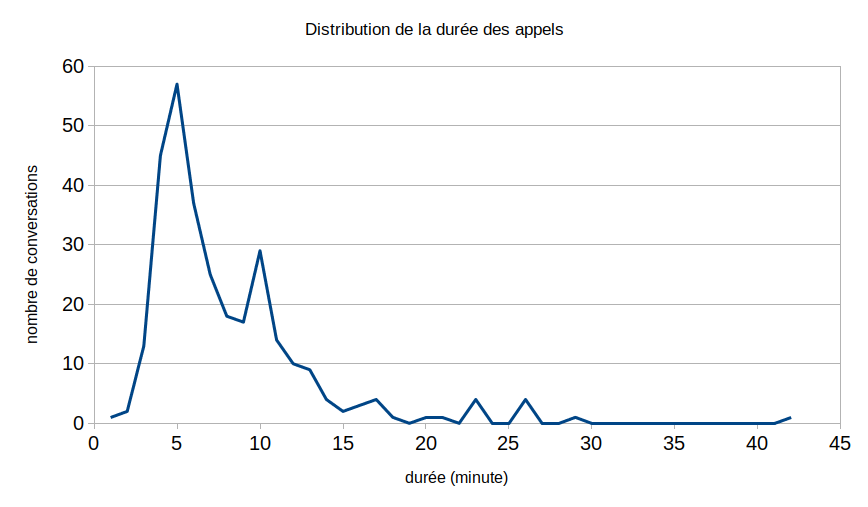
\includegraphics[width=15cm]{./Chapitre4/figures/repart.png}
  \caption{La répartition des conversations en fonction de leur durée. En bleu, nous avons les anciennes durées, en orange les nouvelles. Environ $76,6\%$ des conversations duraient moins de 15 minutes (soit 900 secondes). Après réduction des silences, ce nombre augmente à environ $93,7\%$.}
  \label{fig:repart}
\end{figure}


\subsubsection{Anonymiser les données personnelles}
Afin de respecter la vie privée des clients, la France et d'autres pays européens ont mis en place une réglementation du stockage des données personnelles de tout individu. Le règlement général sur la protection des données (RGPD) établit des règles relatives à la protection des utilisateurs vis à vis du traitement de leur données personnelles, pour s'assurer que les utilisateurs conservent leurs libertés et leurs droits fondamentaux. Cette réglementation, contrôlée par la Commission Nationale de l'Informatique et des Libertés (CNIL) a été renforcée en 2018, afin de mieux protéger les données personnelles des individus.
Nous avons donc obfusqués les données personnelles pour être en adéquation avec les réglementations de la RGPD. Les données personnelles anonymisées sont présentées dans le tableau~\ref{tab:donneesPerso}. À ces dernières s'ajoutent les données permettant d'identifier les entreprises suscitées : les marques et les produits proposées par ces entreprises. Ainsi, les conversations finales permettent de reconnaître le domaine d'activité de l'entreprise mais pas son identité.
Pour procéder à cette obfuscation, une première passe d'un obfuscateur automatique, détenu par la société Allo-Média, a été passée sur les fichiers audio. En reconnaissant les entités nommées sur les transcriptions de ces audios, ce parseur substitue le segment audio correspondant au timecode de l’entité nommée détectée par un signal audio préenregistré qui se compose d'un ait de percussion de type jazzy.
Une deuxième passe, humaine cette fois ci, permet de garantir l'obfuscation de toutes les données personnelles. En utilisant l'outil Transcriber, chaque conversation a été écouté et lu en parallèle, permettant d'identifier et de segmenter les données personnelles encore présentes. C'est lors de cette deuxième phase que les données permettant d'identifier les entreprises ont été isolées. Nous avons également choisi de supprimer tous les numéros permettant d'identifier un contrat ou une date significative.
Les segments identifiés sont alors substitués par le même signal audio jazzy. Une fois ce traitement effectués, nous avons pu passer à l'annotation.

\section{Mise en place de l'annotation}

\subsection{Les deux annotations}
Comme nous l'avons dit précédemment, nous souhaiter analyser l'axe de satisfaction de manière continue. Pour cela, nous avons mis en place un axe dont les extremum sont la frustration (0) et la satisfaction (10) qui passe par un état neutre (5) situé à mi-chemin entre ces deux émotions comme montré dans la figure~\ref{fig:satisfactionAxis}. La valeur de satisfaction est extraite toutes les 250ms, ce qui nous permet d'avoir 4 valeurs par seconde. Nous avons fait ce choix parce que, contrairement aux mots qui seront analysés dans des fenêtres de 30ms pour la reconnaissance automatique de la parole, les émotions s'expriment sur une période de temps plus longue, généralement de l'ordre de la minute~\cite{Schuller2010}. Cette annotation étant influencé par l'affect des annotateurs, nous avons cherché des moyens de valider cette annotation, que ce soit entre différents annotateurs ou même intrinsèque à l'annotateur.

Pour ce faire, nous avons décidé de mettre en place, en plus de l'annotation continue, une annotation discrète de la dimension de satisfaction. Cette annotation discrète est effectuée au niveau de la conversation. Elle relève la catégorie émotionnelle du début et de fin de conversation, comprise entre très frustré, frustré, neutre, satisfait, très satisfait. En plus, une caractérisation de l'évolution de l'émotion est annotée selon les catégories suivante : montante, descendante, stagnante, varie, varie fortement. Pour mieux comprendre ces catégories, elles sont présentées dans la figure~\ref{fig:variation}.
\begin{figure}
  \centering
  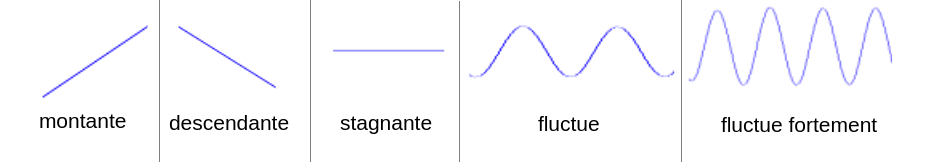
\includegraphics[width=14cm]{./Chapitre4/figures/variation.png}
  \caption{Schéma des variations qui ont été données aux annotateurs afin de mieux comprendre la catégorie évolution}
  \label{fig:variation}
\end{figure}

Dans un objectif de diffusion du corpus, et donc de pouvoir le comprendre aux corpus existant, nous avons également mis en place une annotation de la valence sur le même principe que l'annotation discrète de la dimension de la satisfaction. Elle relève la valence du début et de fin de conversation, comprise entre très négative, négative, neutre, positive, très positive. On y ajoute la même caractérisation de l'évolution de la valence.
La différence entre la dimension de satisfaction et la valence a fait l'objet de plusieurs séances d'explication, afin que ces deux notions ne sont pas confondues par les annotateurs.

\subsection{Contexte donné aux annotateurs}
Afin d'aider les annotateurs et de guider au mieux l'annotation, un guide d'annotation a été mis à leur disposition(disponible dans l'annexe~\ref{ap:guidelines}). Ce dernier explique le contexte de l'étude et les consignes à respecter. Comme l'émotion possède une part non négligeable de subjectivité, il fallait que les consignes soient les plus objectives possibles.
Pour expliquer la notion de valence, nous avons utilisé le Self-Assessment Manikin (SAM)~\cite{SAM} qui donne une description visuelle de la valence, que l'on retrouve sur la figure~\ref{fig:SAM}.
\begin{figure}
  \centering
  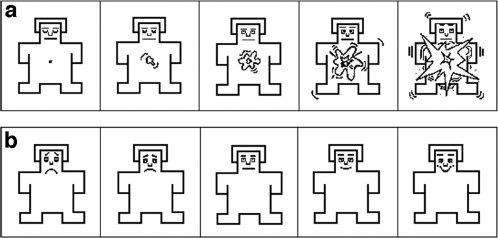
\includegraphics[width=12cm]{./Chapitre4/figures/sam.jpeg}
  \caption{Le Self Assessment Manikin (SAM). La ligne a correspond à l'activation, la ligne b correspond à la valence.}
  \label{fig:SAM}
\end{figure}

Nous nous concentrons sur deux notions :
\begin{itemize}
  \item L'évolution d'une émotion : tous les appels commencent au 'neutre' et évoluent en fonction du temps entre frustration et satisfaction. Cette annotation est continue.
  \item Une évaluation de l'émotion à posteriori : une fois l'appel terminé, nous voulons avoir un retour sur l'évolution de l'émotion. Pour cela nous voulons savoir comment était l'appelant au début de la conversation, comment il était à la fin et comment était l'évolution. Cette annotation est donc discrète.
\end{itemize}

Pour palier à l'aspect subjectif, ils ont été informés que tous les annotateurs annotent les mêmes conversations. Comme l'empathie peut avoir un grand impact sur l'annotation des émotions, nous avons demandé aux annotateurs d'être le plus objectif dans leur annotation et de ne pas prendre partie pour le client.

\subsection{Logiciel utilisé}

Pour réaliser l'annotation continue, CARMA (Continuous Affect Rating And Media Annotation)~\cite{CARMA} est le logiciel d'annotation que nous avons retenu pour cette tâche. Inspiré de FeelTrace~\cite{FeelTrace}, l'outil le plus utilisé pour faire des annotations continues d'émotions, il permet d'annoter de façon continue l'émotion selon une dimension définie en amont. Nous avons choisi CARMA puisque contrairement à FeelTrace, un simple clavier et une souris permettent de mettre en pratique l'annotation. FeelTrace quant à lui, nécessite l'utilisation d'un joystick, qu'il faut se procurer et configurer. De plus, l’outil est optimisé pour annoter deux dimensions à la fois, la valence et l'activation, afin de placer l'annotation dans un contexte bi-dimensionnel qui ne correspond pas avec notre définition de l'axe de satisfaction.

Pour l'annotation discrète, les annotateurs ont rempli un modèle préconstruit vide d'Excel que nous détaillerons par la suite.

\subsection{Consignes}

L'annotation doit être réalisée sur la dimension de satisfaction de façon continue selon les consignes suivantes :
\begin{itemize}
  \item La barre d'annotation va de 0 (Frustration) à 10 (Satisfaction) et est graduée par palier de 1. Le 5 correspond à l'état neutre et à l'état de départ de l'annotation.
  \item Le curseur d'annotation peut être contrôlé par la souris ou par les flèches du clavier. Les pas du clavier sont de 0.1 tandis que la souris peut avoir une granularité plus fine.
  \item Si aucun état émotionnel n'est constaté, ou qu'il ne varie pas, alors l'annotateur ne doit pas toucher à l'annotation. Cela est valable également lors des silences. Les annotateurs ont été notifiés de la présence de conversation où aucun état émotionnel n'a été constaté.
  \item Un document ne doit être annoté qu'une seule fois par la même personne, sans possibilité de revenir en arrière. Il n'est pas non plus possible d'avancer la conversation, l'annotation doit être faite en temps réel de l'écoute de la conversation.
  \item Un document doit être annoté en une seule fois. On ne doit pas revenir à l'annotation d'un fichier après une longue pause (plusieurs heures ou un jour). Cela évite à l'annotateur de ne plus être dans le contexte émotionnel de la conversation.
\end{itemize}

Ces consignes ont pour but d'aider l'annotateur a faire l'annotation la plus objective possible. En plus de ces consignes, la structuration des documents a été expliqué. Les bruit blanc indique qu'un silence de plus de 2 secondes s'est produit. Il a été retiré du document pour fluidifier l'écoute et l'annotation du document. Ce son est à titre informatif pour aider dans l'annotation. Tandis que  les bruits jazzy sont utilisés pour l'anonymisation des conversations. Il remplace les parties de conversation où des données personnelles tel que le nom des personnes ou permettant l'identification de l'entreprise sont prononcées.

Pour leur permettre d'avoir une meilleure compréhension de la satisfaction et de la frustration que nous voulons retrouver, nous avons fourni deux conversations en temps que borne de satisfaction et borne de frustration, afin de calibrer tous les annotateurs, qu'il puisse appréhender l'amplitude potentielle de la dimension de satisfaction.

Pour ce qui est des dimensions discrètes, les consignes stipulent qu'elles doivent être annotées tout de suite après l'écoute de la conversation, afin que les états émotionnels ne soient pas oubliés ou pollués par l'écoute d'autres conversations.
Six catégories sont donc à remplir à la fin de chaque annotation: la dimension de satisfaction de début et de fin de conversation avec la force de l'évolution temporaire; les mêmes informations ont été demandées pour la dimension de la valence.

\section{Analyse de la qualité d'AlloSat}
AlloSat est composé de 303 conversations, d'une durée totale de 37 heures 23 minutes et 27 secondes, et le discours est prononcé par 308 locuteurs distincts dont 191 femmes et 117 hommes.
Ces conversations ont été annotées par trois annotateurs, 2 femmes et 1 homme, formés à la transcription d'appels et à l'annotation en catégorie discrètes de concepts sémantiques.
Une répartition en trois ensembles a été définies. L'ensemble d’entraînement (train) est composé de 201 conversations, le développement de 42 conversations et le test de 60 conversations. De plus amples détails sont disponibles dans le tableau~\ref{tab:repartitionEnSets}.
\begin{table}[]
\begin{tabular}{|l|l|l|l|}
\hline
      & Nombre de conversations & Durée    & Durée de parole \\ \hline
TRAIN & 201                     & 25h26m35 & 15h48m50        \\ \hline
DEV   & 42                      & 05h55m46 & 03h22m14        \\ \hline
TEST  & 60                      & 05h58m41 & 03h28m57        \\ \hline
\end{tabular}
\caption{Découpage du corpus en ensemble de train, développement et test. Les durées sont données en heures, minutes, secondes.}
\label{tab:repartitionEnSets}
\end{table}


Afin de statuer sur la qualité du corpus, nous avons étudiés l'annotation de ces trois annotateurs : nous avons mis en place des mesures d'accord intra-annotateurs, permettant de mesurer la pertinence d'une annotation vis à vis des autres annotations du même annotateur et d'accord inter-annotateurs, permettant de mesure la pertinence de l'annotation d'un document par rapport à une autre annotation du même document.
Le tableau~\ref{tab:statistiqueAnnotation} regroupe l'usage des annotations discrètes de corpus. Nous pouvons observer une sur-représentation de l'état neutre, qui est en adéquation avec la part émotive que l'on s'attendait à trouver dans la parole. Comme nous le pensions, la plupart des conversations ont été perçues avec une frustration croissante, probablement parce que le conseiller n’est pas en mesure de donner une réponse suffisamment satisfaisante à l’interlocuteur.

\subsection{Accord intra-annotateur}
Pour mesurer l'accord intra-annotateur, nous avons choisi de comparer les annotations continues aux annotations discrètes. Comme nous pouvons le voir sur la table~\ref{tab:statistiqueAnnotation}, peu de conversations ont été annotées en très satisfait. Nous avons donc choisi de regrouper les catégories très satisfaites et satisfaites. Afin de rester symétrique dans nos annotations, nous avons également regroupé les catégories très frustrées et frustrées. Les annotations discrètes sont ensuite fusionnées par vote majoritaire. Nous avons eu un cas de désaccord total, dans ce cas nous avons choisi de prendre en compte l'annotation de l'annotateur ayant le plus haut coefficient de corrélation.
Cet accord est mesuré entre les annotations continues et discrètes d'une même conversation par un même annotateur. Les annotations continues ont été normalisées en suivant la méthode de la normalisation min/max, remettant les annotations dans un espace allant de 0 à 1.
Nous avons discrétisés ces valeurs, appelée Sn, pour se synchroniser avec l'annotation discrète. Pour ce faire, nous avons définis deux seuils permettant de déterminer si une valeur continue correspond à un état de frustration (Sn<0.45), à un état neutre (0.45 < Sn < 0.55) ou à un état de satisfaction (Sn > 0.55). Ces seuils ont été définis empiriquement par observation de l'annotation des conversations neutres contenues dans le corpus.
Ensuite nous avons définis les notions de début et fin de conversation dans le contexte de l'annotation continue. Nous avons déterminé qu'il était chacun constitué de 10\% de la durée totale de la conversation. Le début correspond au segment commençant à 0 et finissant à 0.1*durée totale de la conversation et la fin correspond au segment commençant par la durée totale - 0.1*durée de la conversation, jusqu'à la fin de la conversation.
Nous avons alors fait la moyenne des annotations qui représentent le début de la conversation et nous appliquons le seuillage pour déterminer quelle étiquette caractérise cette intervalle de temps. Nous faisons exactement la même chose avec les annotations de fin de conversation. Ainsi pour chaque conversation, nous avons l'annotation discrète effectuée par l'annotateur et une autre annotation discrète correspondant à la discrétisation de son annotation continue.
La différence entre l'annotation discrétisée du début et de la fin devrait être en adéquation avec l'évolution annotée.
Ce processus nous permet de calculer un kappa par annotateur.
Le kappa (k) est une mesure permettant de quantifier l'accord entre deux observations. Elle mesure le degré de concordance entre deux observation selon l'équation suivante\ref{eq:kappa}:
\begin{equation}
    \kappa = \dfrac{P_0 - P_e}{1 - P_e}
    \label{eq:kappa}
\end{equation}
$P_0$ correspond à l'accord relatif entre annotations et $P_e$ représente la probabilité d'un accord aléatoire. Comme nous avons un cas de sur-représentation d'une classe, ici le neutre, nous avons fixé $P_e$ à 1/3~\cite{Callejas2008}.
Le kappa est compris entre 0 et 1. Plus le kappa est proche de 1, plus l'accord entre les deux observations est forte. En revanche, plus le kappa se rapproche de 0 et moins on a d'accord entre les observations.

\begin{table}[th]
  \centering
  \begin{tabular}{|p{2cm}| l l | l l|}
    \hline
        &\multicolumn{2}{c}{\textbf{Nombre de désaccord}} & \multicolumn{2}{c}{\textbf{kappa}} \\
              &début  &fin    &début      &fin  \\
    \hline
    a1        &4      &31     &0.98       &0.84	\\
    a2        &23     &55     &0.88       &0.72 \\
    a3        &13     &50     &0.93       &0.75	\\
    \hline
    Moyenne  &13.33 &45.33 &0.93   &0.77 \\
    \hline
  \end{tabular}
\caption{Nombre de désaccord et kappa pour définir l'accord intra-annotateur pour chacun des trois annotateurs ainsi que la moyenne. $a_i$ represente l'annotateur $i$.}
\label{tab:accordIntraAnnot}
\end{table}

Les résultats de ces calculs sont disponibles dans le tableau~\ref{tab:accordIntraAnnot}. Nous pouvons observer une forte concordance entre les annotations discrètes et les annotations continues discrétisées dans les début de conversation avec un kappa moyen de 0.93. Si on se penche sur le nombre de cas où l'annotation discrète et différente de l'annotation continue discrétisée, on voit que le premier annotateurs et a environ 1\% de différence et qu'au maximum, l'annotateur 2 a une différence de moins de 8\%.
Pour les fins de conversation, on observe de moins bon score, avec un kappa moyen de 0.77 mais qui reste suffisant pour exprimer une cohérence des annotations. En regardant le nombre d'annotations différentes, on observe de nouveau que l'annotateur 1 a le moins de différences avec moins de 10\%, tandis que l'annotateur 2 monte à presque 17\% de différence.
Nous avons conclu que, même si l'accord intra-annotateur n'est pas parfait, il est suffisant pour certifier de la cohérence des annotations produites par un même annotateur : les annotations discrètes et continues sont cohérentes l'une envers l'autre.

\subsection{Accord inter-annotateur}
Afin d’évaluer l’accord inter-annotateur sur les annotations continues, nous avons utilisé le coefficient de corrélation linéaire. Ce coefficient est calculé au niveau de la conversation sur la satisfaction normalisée par rapport à l’ensemble des conversations entre les paires d’annotateurs comme défini dans la section précédente.

Le coefficient de corrélation linéaire donne une mesure de l'intensité et du sens de la relation linéaire entre deux variables, ici les deux annotations de deux annotateurs. Son calcul est définit par l'équation suivante~\ref{eq:coeffCorr}:
\begin{equation}
  R = \dfrac{Cov(x,y)}{\sigma_x*\sigma_y}
  \label{eq:coeffCorr}
\end{equation}
où $Cov(x,y)$ désigne la covariance entre les variables x et y, ici l'ensemble des annotations de deux annotateurs et $\sigma_x$ $\sigma_y$ désignent leur écart type.
Il est compris entre -1 et 1. Plus le coefficient est proche de 1, plus la relation linéaire positive entre les variables est forte. Plus le coefficient est proche de -1, plus la relation linéaire négative entre les variables est forte. Si le coefficient est proche de 0, on ne peut pas établir de relation linéaire.
Nous avons également calculé le kappa entre pair d'annotateur sur les valeurs discrètes de début et de fin de conversation.

\begin{table}[th]
    \centering
    \begin{tabular}{| p{1cm} | l | l l |}
    \hline
      & \multicolumn{1}{c|}{$R$} & \multicolumn{1}{c}{$\kappa^{début}$} & \multicolumn{1}{c}{$\kappa^{fin}$}\\
      \hline
      a1-a2   &0.82   &0.99   &0.90   \\
      a2-a3   &0.87   &0.88   &0.69   \\
      a1-a3   &0.80   &0.87   &0.72   \\
      \hline
      Moyenne &0.83   &0.91   &0.77   \\
      \hline
    \end{tabular}
    \caption{Accord inter-annotateur calculé entre les pairs d'annotateurs ainsi que la moyenne.$a_i$ représente l'annotateur $i$. $R$ represente le coefficient de corrélation, \kappa représente le kappa de début et de fin de conversation.}
    \label{tab:accordInterAnnot}
  \end{table}

Les valeurs finales rapportées dans le tableau~\ref{accordInterAnnot} montrent une bonne corrélation entre les annotateurs (un coefficient de corrélation moyen de 0,83), ce qui signifie que les annotations continues sont cohérentes entre les annotateurs.
On observe toutefois que l'annotateur 1 et l'annotateur 3 sont moins enclin à donner les mêmes annotations que les pairs d'annotateurs 1;2 et 2;3. On remarque également que le kappa de début de conversation est très élevé. L’une des raisons de ce fort accord est que le début de la conversation est presque toujours neutre. Cela peut s’expliquer de deux façons : tout d’abord, l’annotation continue est toujours initialisée à 5, ce qui se traduit par un état neutre. Nous avons donc un biais introduit par cet état initial, qui permet à toutes les annotations de commencer de la même manière.
Mais l’hypothèse principale est que l’interlocuteur est rarement frustré au début de l’appel : cette émotion est provoquée par les réponses de l’agent. Il en va de même pour la satisfaction. En partant de ces résultats d’accord prometteurs, nous calculons une annotation de référence pour chaque conversation correspondant à la moyenne des trois annotations de la satisfaction et nous pouvons utiliser cette annotation de référence à des fins d’analyse et d’apprentissage. Cette annotation de référence, aussi appelée annotation gold, est utilisée dans les expériences présentées par la suite.
D'autres stratégies de fusion d'annotation existent, permettant de mettre un poids plus important à un annotateur ou à lisser les grands écarts d'annotation, mais devant nos résultats d'accord intra et inter-annotateurs, nous avons décidé d'utiliser la fusion d'annotation la plus simple, pour ne pas influencer les futures systèmes de reconnaissance automatique.

\section{Calcul du CCC entre annotateurs}
Afin d'asseoir notre analyse de la cohérence d'annotation, nous avons également décidés de calculer le score CCC entre les annotateurs et l'annotation de référence correspondant à la moyenne de leurs observations.
Comme nous l'avons expliqué dans le chapitre 3~\ref{chapitre3}, Le CCC permet d'évaluer la performance des systèmes de reconnaissances automatique des émotions. Nous avons donc fait l'hypothèse que l'évaluation de nos annotations avec cette métrique nous permettrait de mettre en place une comparaison entre la performance d'un système automatique et la performance d'un humain.
Ce score a été calculé de deux façons. Dans un premier temps, nous avons déterminé un score global de l'annotateur. Puis nous avons voulu aller plus loin et calculer un score à chacun des conversations, pour déterminer les documents dont l'annotation étaient les plus différentes.

\begin{table}
  \centering
  \begin{tabular}{|l|c|}
  \hline
  a1       &0.815 \\
  a2       &0.944 \\
  a3       &0.918 \\
  \hline
  \end{tabular}
  \caption{Score CCC calculé entre les annotations des annotateurs $a_i$ et l'annotation de référence.}
  \label{tab:cccEntreAnnotateurs}
\end{table}

Les scores de CCC sont disponibles dans le tableau~\ref{tab:cccEntreAnnotateurs}. On peut remarquer que les scores sont très bons, allant de 0.815 à 0.944 selon les annotateurs. Ces bons scores sont tout à fait logiques puisque l'annotation de référence est issue de l'annotation de ces trois annotations. On peut alors prendre plusieurs positionnements:
\begin{itemize}
  \item On peut considérer qu'un score supérieur à 0.815 correspond à un bon score de reconnaissance puisqu'il est au niveau du "plus mauvais" de nos humains,
  \item sinon on peut considérer qu'un score de 0.892, moyenne de ces trois scores, correspond au score atteignable en moyenne par l'humain, et que donc si la reconnaissance automatique dépasse ce score, elle est au moins autant performante que l'humain,
  \item ou finalement, si le système de reconnaissance a un score supérieur à 0.944, il est plus performant que "le meilleur" de nos humains et donc qu'il est meilleur que l'homme pour annoter la satisfaction et la frustration.
\end{itemize}

Nous avons décidé de suivre la deuxième conjonction. Ainsi, si le système atteint un score supérieur à 0.892, on peut considérer qu'il est autant performant que l'humain dans la tache de reconnaissance de la satisfaction et de la frustration.

En regardant les scores de chaque conversation, représenté dans le tableau~\ref{tab:tousScoresAnnotateurs}, nous avons pu déterminer X conversations qui sont annotées de façon différente par les annotateurs.

\begin{table}[]
\begin{tabular}{|l|l|l|l|l|}
\hline
Conversation     & laure a1 & jf a2 & nathalie a3 & moyenne \\ \hline
Conversation 1   & 0.682    & 0.911 & 0.930       & 0.841   \\ \hline
Conversation 2   & 0.704    & 0.91  & 0.841       & 0.818   \\ \hline
Conversation 3   & 0.726    & 0.931 & 0.789       & 0.816   \\ \hline
Conversation 4   & 0        & 0.341 & 0           & 0.114   \\ \hline
Conversation 5   & 0.903    & 0.976 & 0.970       & 0.950   \\ \hline
Conversation 6   & 0.841    & 0.482 & 0.201       & 0.508   \\ \hline
Conversation 7   & 0.255    & 0.247 & 0.377       & 0.293   \\ \hline
Conversation 8   & 0.909    & 0.924 & 0.928       & 0.920   \\ \hline
Conversation 9   & 0.767    & 0.929 & 0.772       & 0.823   \\ \hline
Conversation 10  & 0.002    & 0.598 & 0.002       & 0.201   \\ \hline
Conversation 11  & 0        & 0.515 & 0.563       & 0.359   \\ \hline
Conversation 12  & 0.910    & 0.978 & 0.981       & 0.956   \\ \hline
Conversation 13  & 0        & 0.241 & 0.539       & 0.260   \\ \hline
Conversation 14  & 0.831    & 0.986 & 0.900       & 0.906   \\ \hline
Conversation 15  & 0.746    & 0.942 & 0.919       & 0.869   \\ \hline
Conversation 16  & 0.404    & 0.915 & 0.817       & 0.712   \\ \hline
Conversation 17  & 0        & 0.501 & 0           & 0.167   \\ \hline
Conversation 18  & 0.724    & 0.955 & 0.913       & 0.864   \\ \hline
Conversation 19  & 0.761    & 0.968 & 0.858       & 0.862   \\ \hline
Conversation 20  & 0.624    & 0.962 & 0.855       & 0.814   \\ \hline
Conversation 21  & 0.582    & 0.974 & 0.814       & 0.790   \\ \hline
Conversation 22  & 0.847    & 0.649 & 0.741       & 0.746   \\ \hline
Conversation 23  & 0.741    & 0.940 & 0.934       & 0.872   \\ \hline
Conversation 24  & 0.716    & 0.879 & 0.942       & 0.846   \\ \hline
Conversation 25  & 0.825    & 0.821 & 0           & 0.549   \\ \hline
Conversation 26  & 0.774    & 0.962 & 0.853       & 0.863   \\ \hline
Conversation 27  & 0.637    & 0.868 & 0.972       & 0.825   \\ \hline
Conversation 28  & 0.827    & 0.858 & 0.909       & 0.865   \\ \hline
Conversation 29  & 0.154    & 0.680 & 0.810       & 0.548   \\ \hline
Conversation 30  & 0.640    & 0.937 & 0.769       & 0.782   \\ \hline
Conversation 31  & 0.678    & 0.952 & 0.908       & 0.846   \\ \hline
Conversation 32  & 0.338    & 0.867 & 0.843       & 0.683   \\ \hline
Conversation 33  & 0.512    & 0.929 & 0.872       & 0.771   \\ \hline
Conversation 34  & 0.268    & 0.771 & 0.731       & 0.590   \\ \hline
Conversation 35  & 0.583    & 0.892 & 0.917       & 0.798   \\ \hline
Conversation 36  & 0        & 0.244 & 0           & 0.081   \\ \hline
Conversation 37  & 0        & 0.687 & 0.686       & 0.458   \\ \hline
Conversation 38  & 0.969    & 0.969 & 0.971       & 0.970   \\ \hline
Conversation 39  & 0        & 0.627 & 0.815       & 0.480   \\ \hline
Conversation 40  & 0        & 0.258 & 0.019       & 0.092   \\ \hline
Conversation 41  & 0        & 0.481 & 0.683       & 0.388   \\ \hline
Conversation 42  & 0.920    & 0.980 & 0.957       & 0.952   \\ \hline
Conversation 43  & 0.696    & 0.780 & 0.856       & 0.777   \\ \hline
Conversation 44  & 0.743    & 0.893 & 0.767       & 0.801   \\ \hline
Conversation 45  & 0.959    & 0.864 & 0.902       & 0.908   \\ \hline
Conversation 46  & 0        & 0.247 & 0           & 0.082   \\ \hline
Conversation 47  & 0.686    & 0.591 & 0.274       & 0.517   \\ \hline
Conversation 48  & 0        & 0.417 & 0           & 0.139   \\ \hline
Conversation 49  & 0.561    & 0.415 & 0.412       & 0.463   \\ \hline
Conversation 50  & 0.787    & 0.953 & 0.841       & 0.860   \\ \hline
Conversation 51  & 0.943    & 0.863 & 0.904       & 0.903   \\ \hline
Conversation 52  & 0.542    & 0.931 & 0.763       & 0.745   \\ \hline
Conversation 53  & 0.669    & 0.916 & 0.933       & 0.840   \\ \hline
Conversation 54  & 0        & 0.389 & 0.587       & 0.325   \\ \hline
Conversation 55  & 0        & 0.233 & 0           & 0.078   \\ \hline
Conversation 56  & 0        & 0.734 & 0.845       & 0.526   \\ \hline
Conversation 57  & 0.752    & 0.945 & 0.823       & 0.840   \\ \hline
Conversation 58  & 0.967    & 0.905 & 0.912       & 0.928   \\ \hline
Conversation 59  & 0.689    & 0.977 & 0.897       & 0.854   \\ \hline
Conversation 60  & 0.839    & 0.966 & 0.859       & 0.888   \\ \hline
Conversation 61  & 0        & 0.443 & 0.182       & 0.208   \\ \hline
Conversation 62  & 0        & 0.58  & 0.730       & 0.437   \\ \hline
Conversation 63  & 0        & 0.436 & 0.436       & 0.291   \\ \hline
Conversation 64  & 0.271    & 0.953 & 0.792       & 0.672   \\ \hline
Conversation 65  & 0        & 0.168 & 0.257       & 0.142   \\ \hline
Conversation 66  & 0.636    & 0.957 & 0.837       & 0.810   \\ \hline
Conversation 67  & 0.621    & 0.975 & 0.805       & 0.800   \\ \hline
Conversation 68  & 0.824    & 0.972 & 0.893       & 0.896   \\ \hline
Conversation 69  & 0.688    & 0.796 & 0.870       & 0.784   \\ \hline
Conversation 70  & 0.964    & 0.923 & 0.969       & 0.952   \\ \hline
Conversation 71  & 0        & 0.547 & 0.303       & 0.284   \\ \hline
Conversation 72  & 0.858    & 0.992 & 0.911       & 0.920   \\ \hline
Conversation 73  & 0        & 0.619 & 0.522       & 0.381   \\ \hline
Conversation 74  & 0.350    & 0.264 & 0.052       & 0.222   \\ \hline
Conversation 75  & 0.700    & 0.985 & 0.765       & 0.817   \\ \hline
Conversation 76  & 0.885    & 0.980 & 0.875       & 0.913   \\ \hline
Conversation 77  & 0        & 0.203 & 0.406       & 0.203   \\ \hline
Conversation 78  & 0        & 0.394 & 0.455       & 0.283   \\ \hline
Conversation 79  & 0        & 0.890 & 0.681       & 0.523   \\ \hline
Conversation 80  & 0        & 0.259 & 0           & 0.086   \\ \hline
Conversation 81  & 0        & 0.752 & 0.788       & 0.513   \\ \hline
Conversation 82  & 0        & 0.525 & 0           & 0.175   \\ \hline
Conversation 83  & 0        & 0.151 & 0.173       & 0.108   \\ \hline
Conversation 84  & 0.944    & 0.957 & 0.919       & 0.940   \\ \hline
Conversation 85  & 0.486    & 0.447 & 0.110       & 0.348   \\ \hline
Conversation 86  & 0        & 0.314 & 0           & 0.105   \\ \hline
Conversation 87  & 0        & 0.390 & 0.490       & 0.293   \\ \hline
Conversation 88  & 0.721    & 0.970 & 0.922       & 0.871   \\ \hline
Conversation 89  & 0.766    & 0.770 & 0.934       & 0.823   \\ \hline
Conversation 90  & 0.938    & 0.943 & 0.920       & 0.934   \\ \hline
Conversation 91  & 0.799    & 0.969 & 0.891       & 0.886   \\ \hline
Conversation 92  & 0        & 0.355 & 0           & 0.118   \\ \hline
Conversation 93  & 0.713    & 0.959 & 0.913       & 0.862   \\ \hline
Conversation 94  & 0        & 0.501 & 0.791       & 0.431   \\ \hline
Conversation 95  & 0        & 0.835 & 0.742       & 0.526   \\ \hline
Conversation 96  & 0.501    & 0.953 & 0.749       & 0.734   \\ \hline
Conversation 97  & 0        & 0.699 & 0.761       & 0.487   \\ \hline
Conversation 98  & 0.952    & 0.907 & 0.859       & 0.906   \\ \hline
Conversation 99  & 0        & 0.893 & 0.783       & 0.559   \\ \hline
Conversation 100 & 0.797    & 0.850 & 0.867       & 0.838   \\ \hline
Conversation 101 & 0.768    & 0.111 & 0.767       & 0.549   \\ \hline
Conversation 102 & 0        & 0.822 & 0.692       & 0.505   \\ \hline
Conversation 103 & 0        & 0.601 & 0.631       & 0.411   \\ \hline
Conversation 104 & 0        & 0.337 & 0.727       & 0.355   \\ \hline
Conversation 105 & 0.655    & 0.950 & 0.849       & 0.818   \\ \hline
Conversation 106 & 0.837    & 0.953 & 0.915       & 0.902   \\ \hline
Conversation 107 & 0.001    & 0.580 & 0.001       & 0.194   \\ \hline
Conversation 108 & 0.910    & 0.976 & 0.918       & 0.934   \\ \hline
Conversation 109 & 0.538    & 0.581 & 0.695       & 0.605   \\ \hline
Conversation 110 & 0.583    & 0.819 & 0.979       & 0.794   \\ \hline
Conversation 111 & 0.869    & 0.829 & 0.792       & 0.830   \\ \hline
Conversation 112 & 0        & 0.699 & 0.589       & 0.429   \\ \hline
Conversation 113 & 0.417    & 0.965 & 0.701       & 0.694   \\ \hline
Conversation 114 & 0.933    & 0.940 & 0.934       & 0.935   \\ \hline
Conversation 115 & 0.887    & 0.971 & 0.925       & 0.928   \\ \hline
Conversation 116 & 0.385    & 0.889 & 0.856       & 0.710   \\ \hline
Conversation 117 & 0.710    & 0.948 & 0.908       & 0.855   \\ \hline
Conversation 118 & 0.896    & 0.978 & 0.933       & 0.936   \\ \hline
Conversation 119 & 0.975    & 0.742 & 0.919       & 0.879   \\ \hline
Conversation 120 & 0.984    & 0.981 & 0.983       & 0.983   \\ \hline
Conversation 121 & 0        & 0.819 & 0.784       & 0.535   \\ \hline
Conversation 122 & 0.594    & 0.970 & 0.857       & 0.807   \\ \hline
Conversation 123 & 0.724    & 0.981 & 0.761       & 0.822   \\ \hline
Conversation 124 & 0        & 0.727 & 0.775       & 0.501   \\ \hline
Conversation 125 & 0.805    & 0.978 & 0.856       & 0.879   \\ \hline
Conversation 126 & 0.940    & 0.954 & 0.927       & 0.940   \\ \hline
Conversation 127 & 0.385    & 0.955 & 0.693       & 0.678   \\ \hline
Conversation 128 & 0.931    & 0.971 & 0.895       & 0.932   \\ \hline
Conversation 129 & 0.770    & 0.910 & 0.970       & 0.884   \\ \hline
Conversation 130 & 0.913    & 0.633 & 0.816       & 0.787   \\ \hline
Conversation 131 & 0.964    & 0.833 & 0.839       & 0.879   \\ \hline
Conversation 132 & 0        & 0.207 & 0           & 0.069   \\ \hline
Conversation 133 & 0.834    & 0.968 & 0.958       & 0.920   \\ \hline
Conversation 134 & 0        & 0.316 & 0           & 0.105   \\ \hline
Conversation 135 & 0.880    & 0.941 & 0.955       & 0.925   \\ \hline
Conversation 136 & 0        & 0.949 & 0.643       & 0.531   \\ \hline
Conversation 137 & 0        & 0.205 & 0.165       & 0.124   \\ \hline
Conversation 138 & 0        & 0.469 & 0           & 0.156   \\ \hline
Conversation 139 & 0.902    & 0.965 & 0.969       & 0.945   \\ \hline
Conversation 140 & 0.468    & 0.899 & 0.918       & 0.761   \\ \hline
Conversation 141 & 0.645    & 0.951 & 0.850       & 0.815   \\ \hline
Conversation 142 & 0.756    & 0.969 & 0.886       & 0.870   \\ \hline
Conversation 143 & 0        & 0.548 & 0.692       & 0.413   \\ \hline
Conversation 144 & 0        & 0.555 & 0           & 0.185   \\ \hline
Conversation 145 & 0.579    & 0.900 & 0.937       & 0.805   \\ \hline
Conversation 146 & 0        & 0.356 & 0.623       & 0.326   \\ \hline
Conversation 147 & 0.884    & 0.627 & 0.375       & 0.629   \\ \hline
Conversation 148 & 0.915    & 0.901 & 0.925       & 0.914   \\ \hline
Conversation 149 & 0.722    & 0.971 & 0.818       & 0.837   \\ \hline
Conversation 150 & 0        & 0.460 & 0           & 0.154   \\ \hline
Conversation 151 & 0.513    & 0.839 & 0.627       & 0.660   \\ \hline
Conversation 152 & 0.720    & 0.663 & 0.826       & 0.737   \\ \hline
Conversation 153 & 0.840    & 0.950 & 0.961       & 0.917   \\ \hline
Conversation 154 & 0        & 0.242 & 0           & 0.081   \\ \hline
Conversation 155 & 0.080    & 0.538 & 0.645       & 0.421   \\ \hline
Conversation 156 & 0.715    & 0.872 & 0.880       & 0.822   \\ \hline
Conversation 157 & 0.586    & 0.949 & 0.782       & 0.772   \\ \hline
Conversation 158 & 0.656    & 0.918 & 0.884       & 0.819   \\ \hline
Conversation 159 & 0.762    & 0.699 & 0.779       & 0.747   \\ \hline
Conversation 160 & 0.939    & 0.910 & 0.977       & 0.942   \\ \hline
Conversation 161 & 0        & 0.955 & 0.850       & 0.602   \\ \hline
Conversation 162 & 0.871    & 0.951 & 0.937       & 0.920   \\ \hline
Conversation 163 & 0.882    & 0.958 & 0.984       & 0.941   \\ \hline
Conversation 164 & 0.852    & 0.488 & 0.601       & 0.647   \\ \hline
Conversation 165 & 0        & 0.849 & 0.594       & 0.481   \\ \hline
Conversation 166 & 0.534    & 0.782 & 0.872       & 0.729   \\ \hline
Conversation 167 & 0.966    & 0.758 & 0.884       & 0.869   \\ \hline
Conversation 168 & 0.940    & 0.960 & 0.975       & 0.958   \\ \hline
Conversation 169 & 0.999    & 0.999 & 0.999       & 0.999   \\ \hline
Conversation 170 & 0.894    & 0.986 & 0.947       & 0.942   \\ \hline
Conversation 171 & 0.818    & 0.843 & 0.870       & 0.844   \\ \hline
Conversation 172 & 0.989    & 0.908 & 0.910       & 0.936   \\ \hline
Conversation 173 & 0.793    & 0.983 & 0.862       & 0.879   \\ \hline
Conversation 174 & 0        & 0.823 & 0.506       & 0.443   \\ \hline
Conversation 175 & 0.538    & 0.877 & 0.919       & 0.778   \\ \hline
Conversation 176 & 0.643    & 0.793 & 0.846       & 0.761   \\ \hline
Conversation 177 & 0.555    & 0.918 & 0.870       & 0.781   \\ \hline
Conversation 178 & 0.744    & 0.786 & 0.790       & 0.773   \\ \hline
Conversation 179 & 0.001    & 0.434 & 0.001       & 0.145   \\ \hline
Conversation 180 & 0        & 0.944 & 0.702       & 0.549   \\ \hline
Conversation 181 & 0.590    & 0.507 & 0.782       & 0.626   \\ \hline
Conversation 182 & 0.839    & 0.848 & 0.801       & 0.829   \\ \hline
Conversation 183 & 0        & 0.163 & 0           & 0.054   \\ \hline
Conversation 184 & 0        & 0.456 & 0.757       & 0.405   \\ \hline
Conversation 185 & 0.484    & 0.816 & 0.648       & 0.650   \\ \hline
Conversation 186 & 0.768    & 0.957 & 0.912       & 0.879   \\ \hline
Conversation 187 & 0        & 0.363 & 0           & 0.121   \\ \hline
Conversation 188 & 0.734    & 0.945 & 0.937       & 0.872   \\ \hline
Conversation 189 & 0.965    & 0.981 & 0.967       & 0.971   \\ \hline
Conversation 190 & 0        & 0.573 & 0.802       & 0.458   \\ \hline
Conversation 191 & 0.211    & 0.486 & 0.629       & 0.442   \\ \hline
Conversation 192 & 0.975    & 0.908 & 0.943       & 0.942   \\ \hline
Conversation 193 & 0.941    & 0.951 & 0.912       & 0.935   \\ \hline
Conversation 194 & 0.487    & 0.979 & 0.836       & 0.767   \\ \hline
Conversation 195 & 0.474    & 0.882 & 0.886       & 0.748   \\ \hline
Conversation 196 & 0.686    & 0.794 & 0.789       & 0.756   \\ \hline
Conversation 197 & 0.902    & 0.890 & 0.871       & 0.888   \\ \hline
Conversation 198 & 0.852    & 0.967 & 0.938       & 0.919   \\ \hline
Conversation 199 & 0.623    & 0.984 & 0.804       & 0.804   \\ \hline
Conversation 200 & 0.430    & 0.898 & 0.840       & 0.723   \\ \hline
Conversation 201 & 0.365    & 0.810 & 0.844       & 0.673   \\ \hline
Conversation 202 & 0.700    & 0.903 & 0.933       & 0.845   \\ \hline
Conversation 203 & 0.917    & 0.892 & 0.873       & 0.894   \\ \hline
Conversation 204 & 0.737    & 0.910 & 0.856       & 0.834   \\ \hline
Conversation 205 & 0.951    & 0.935 & 0.911       & 0.932   \\ \hline
Conversation 206 & 0.804    & 0.968 & 0.949       & 0.907   \\ \hline
Conversation 207 & 0.398    & 0.694 & 0.785       & 0.626   \\ \hline
Conversation 208 & 0.701    & 0.968 & 0.920       & 0.863   \\ \hline
Conversation 209 & 0.980    & 0.688 & 0.850       & 0.839   \\ \hline
Conversation 210 & 0.744    & 0.966 & 0.800       & 0.837   \\ \hline
Conversation 211 & 0.974    & 0.987 & 0.977       & 0.979   \\ \hline
Conversation 212 & 0.684    & 0.439 & 0.839       & 0.654   \\ \hline
Conversation 213 & 0.820    & 0.785 & 0.902       & 0.836   \\ \hline
Conversation 214 & 0        & 0.250 & 0           & 0.083   \\ \hline
Conversation 215 & 0.631    & 0.974 & 0.808       & 0.804   \\ \hline
Conversation 216 & 0.800    & 0.979 & 0.923       & 0.901   \\ \hline
Conversation 217 & 0.511    & 0.983 & 0.752       & 0.749   \\ \hline
Conversation 218 & 0.468    & 0.924 & 0.712       & 0.701   \\ \hline
Conversation 219 & 0        & 0.558 & 0.870       & 0.476   \\ \hline
Conversation 220 & 0        & 0.506 & 0.386       & 0.297   \\ \hline
Conversation 221 & 0        & 0.353 & 0           & 0.118   \\ \hline
Conversation 222 & 0        & 0.294 & 0           & 0.098   \\ \hline
Conversation 223 & 0.729    & 0.948 & 0.823       & 0.833   \\ \hline
Conversation 224 & 0.919    & 0.977 & 0.924       & 0.940   \\ \hline
Conversation 225 & 0.820    & 0.83  & 0.842       & 0.831   \\ \hline
Conversation 226 & 0.767    & 0.953 & 0.810       & 0.843   \\ \hline
Conversation 227 & 0        & 0.259 & 0.292       & 0.184   \\ \hline
Conversation 228 & 0        & 0.204 & 0.405       & 0.203   \\ \hline
Conversation 229 & 0.779    & 0.978 & 0.925       & 0.894   \\ \hline
Conversation 230 & 0        & 0.250 & 0           & 0.083   \\ \hline
Conversation 231 & 0        & 0.752 & 0.602       & 0.452   \\ \hline
Conversation 232 & 0.920    & 0.956 & 0.960       & 0.945   \\ \hline
Conversation 233 & 0.875    & 0.932 & 0.875       & 0.894   \\ \hline
Conversation 234 & 0.542    & 0.985 & 0.819       & 0.782   \\ \hline
Conversation 235 & 0.731    & 0.953 & 0.899       & 0.861   \\ \hline
Conversation 236 & 0.529    & 0.951 & 0.732       & 0.737   \\ \hline
Conversation 237 & 0.463    & 0.206 & 0           & 0.223   \\ \hline
Conversation 238 & 0.750    & 0.407 & 0.862       & 0.673   \\ \hline
Conversation 239 & 0        & 0.428 & 0.540       & 0.323   \\ \hline
Conversation 240 & 0.923    & 0.954 & 0.975       & 0.951   \\ \hline
Conversation 241 & 0        & 0.905 & 0.744       & 0.550   \\ \hline
Conversation 242 & 0        & 0.340 & 0.189       & 0.176   \\ \hline
Conversation 243 & 0        & 0.421 & 0.699       & 0.374   \\ \hline
Conversation 244 & 0.919    & 0.969 & 0.936       & 0.941   \\ \hline
Conversation 245 & 0        & 0.668 & 0.901       & 0.523   \\ \hline
Conversation 246 & 0.297    & 0.731 & 0.759       & 0.596   \\ \hline
Conversation 247 & 0.913    & 0.894 & 0.756       & 0.854   \\ \hline
Conversation 248 & 0.690    & 0.820 & 0.632       & 0.714   \\ \hline
Conversation 249 & 0.108    & 0.784 & 0.418       & 0.437   \\ \hline
Conversation 250 & 0.946    & 0.942 & 0.942       & 0.944   \\ \hline
Conversation 251 & 0.676    & 0.970 & 0.860       & 0.835   \\ \hline
Conversation 252 & 0.671    & 0.951 & 0.895       & 0.839   \\ \hline
Conversation 253 & 0.850    & 0.977 & 0.886       & 0.904   \\ \hline
Conversation 254 & 0.732    & 0.933 & 0.063       & 0.576   \\ \hline
Conversation 255 & 0.921    & 0.878 & 0.964       & 0.921   \\ \hline
Conversation 256 & 0.663    & 0.987 & 0.867       & 0.839   \\ \hline
Conversation 257 & 0.730    & 0.939 & 0.919       & 0.863   \\ \hline
Conversation 258 & 0.780    & 0.539 & 0.124       & 0.481   \\ \hline
Conversation 259 & 0.749    & 0.844 & 0.972       & 0.855   \\ \hline
Conversation 260 & 0        & 0.681 & 0.728       & 0.469   \\ \hline
Conversation 261 & 0.555    & 0.958 & 0.822       & 0.779   \\ \hline
Conversation 262 & 0.737    & 0.951 & 0.924       & 0.871   \\ \hline
Conversation 263 & 0.846    & 0.938 & 0.811       & 0.865   \\ \hline
Conversation 264 & 0.520    & 0.933 & 0.879       & 0.777   \\ \hline
Conversation 265 & 0.772    & 0.970 & 0.870       & 0.871   \\ \hline
Conversation 266 & 0        & 0.175 & 0           & 0.058   \\ \hline
Conversation 267 & 0.507    & 0.276 & 0.615       & 0.466   \\ \hline
Conversation 268 & 0.926    & 0.940 & 0.939       & 0.935   \\ \hline
Conversation 269 & 0        & 0.233 & 0           & 0.078   \\ \hline
Conversation 270 & 0.494    & 0.915 & 0.800       & 0.736   \\ \hline
Conversation 271 & 0.306    & 0.840 & 0.548       & 0.565   \\ \hline
Conversation 272 & 0        & 0.207 & 0           & 0.069   \\ \hline
Conversation 273 & 0.900    & 0.965 & 0.959       & 0.941   \\ \hline
Conversation 274 & 0.822    & 0.972 & 0.883       & 0.893   \\ \hline
Conversation 275 & 0.907    & 0.935 & 0.881       & 0.908   \\ \hline
Conversation 276 & 0.643    & 0.496 & 0.857       & 0.665   \\ \hline
Conversation 277 & 0.264    & 0.779 & 0.387       & 0.476   \\ \hline
Conversation 278 & 0.592    & 0.970 & 0.837       & 0.800   \\ \hline
Conversation 279 & 0.677    & 0.856 & 0.982       & 0.838   \\ \hline
Conversation 280 & 0.776    & 0.941 & 0.936       & 0.884   \\ \hline
Conversation 281 & 0        & 0.855 & 0.851       & 0.568   \\ \hline
Conversation 282 & 0.572    & 0.745 & 0.799       & 0.705   \\ \hline
Conversation 283 & 0        & 0.696 & 0.826       & 0.507   \\ \hline
Conversation 284 & 0        & 0.300 & 0           & 0.100   \\ \hline
Conversation 285 & 0.751    & 0.773 & 0.773       & 0.766   \\ \hline
Conversation 286 & 0        & 0.372 & 0           & 0.124   \\ \hline
Conversation 287 & 0.676    & 0.984 & 0.861       & 0.840   \\ \hline
Conversation 288 & 0.815    & 0.970 & 0.825       & 0.870   \\ \hline
Conversation 289 & 0.697    & 0.430 & 0.712       & 0.613   \\ \hline
Conversation 290 & 0.757    & 0.969 & 0.883       & 0.870   \\ \hline
Conversation 291 & 0        & 0.390 & 0.105       & 0.165   \\ \hline
Conversation 292 & 0        & 0.418 & 0           & 0.139   \\ \hline
Conversation 293 & 0.638    & 0.909 & 0.804       & 0.784   \\ \hline
Conversation 294 & 0.488    & 0.627 & 0.866       & 0.660   \\ \hline
Conversation 295 & 0.895    & 0.715 & 0.758       & 0.789   \\ \hline
Conversation 296 & 0.352    & 0.886 & 0.772       & 0.670   \\ \hline
Conversation 297 & 0        & 0.365 & 0           & 0.122   \\ \hline
Conversation 298 & 0        & 0.483 & 0.588       & 0.357   \\ \hline
Conversation 299 & 0.669    & 0.846 & 0.972       & 0.829   \\ \hline
Conversation 300 & 0.527    & 0.659 & 0.843       & 0.676   \\ \hline
Conversation 301 & 0.729    & 0.877 & 0.956       & 0.854   \\ \hline
Conversation 302 & 0.676    & 0.756 & 0.752       & 0.728   \\ \hline
Conversation 303 & 0        & 0.330 & 0           & 0.110   \\ \hline
\end{tabular}
\label{tab:tousScoresAnnotateurs}
\caption{Tous les scores calculés entre l'annotation de référence et l'annotation de l'annotateur $a_i$. }
\end{table}


\subsection{Étude empirique sur une fraction du corpus}

\subsubsection{Redondance de signal et silences}
Nous avons étudiés la répartition de nos ensembles. Nous avons observé qu'il y avait plus de fichiers courts en durée dans notre set de test. En effet, en moyenne un fichier du set de test dure 363 secondes alors qu'un fichier de train dure 464 secondes et un fichier de développement 492 secondes comme explicité dans le tableau~\ref{tab:durée}.
\begin{table}[]
    \centering
    \begin{tabular}{|p{3cm}|c c c |}
        \hline
          &Train &Dev &Test \\
         \hline
         < 7min &99 &18 &38 \\
         > 7min &101 &24 &22 \\
         \hline
         < 5min &40 &4 &17 \\
         > 5min &160 &38 &43 \\
         \hline
    \end{tabular}
    \caption{Répartition de la durée des conversations en fonction des sets considérés}
    \label{tab:durée}
\end{table}


Nous avons également pris en considération les silences que nous avons rajoutés artificiellement lors de la création du corpus. En effet, comme nous n'avons pas les interventions du conseiller, nous avions des silences très long, qu'ils n'étaient pas nécessaires de faire annoter. Nous les avons donc supprimé et remplacé par deux secondes de bruits blancs. Or nous nous posions la question de savoir si cet ajout était bien balancé au sein de nos ensembles. Nous avons constaté que cet ajout était plutot bien balancé dans nos ensembles en effet il y a en moyenne 41.82 bruit blanc par conversation dans le train, 40.79 dans le développement et 36.32 dans le test.
Les trois ensembles ont donc un traitement des silences dans la même ordre de grandeur.

\subsection{Écoute humaine}
Afin de mieux comprendre les données, nous avons choisi d'écouter 57 conversations choisies au hasard dans le corpus. Ces 57 conversations proviennent indépendamment du train, développement et test.
Plusieurs phénomènes ont été observés sur ces conversations, mais nous n'avons pas trouvé un indicateur commun à celles-ci. En effet, ces conversations contiennent ou non du bruit, de la musique, plusieurs locuteurs, des rires, des voix âgées, des silences plutôt marquées (en début, milieu ou fin de conversations) et de la frustration manifeste (augmentation du débit de parole, du volume, moins de temps de silence, injures,...). Le nombre de ces paramètres retrouvés sont résumés dans le tableau~\ref{tab:ecouteHumaine}. De plus, nous y avons ajouté des données sur le sexe du locuteur, les domaines des conversations et la variabilité de l'annotation.
Nous n'avons pas trouvé de schéma clair et universel de la dimension de satisfaction avec ces observations.

\section{Modalités de diffusion du corpus}
Le corpus est diffusable à toute personne affiliée à un institut public de recherche sur simple demande. En effet, Allo-Média et le laboratoire informatique de l'université du mans ont statué sur la méthode de diffusion du corpus.
Ce dernier peut être demandé par mail aux personnes responsables de sa diffusion, à savoir Anthony Rousseau (a.rousseau@allo-media.fr), Marie Tahon (m.tahon@univ-lemans.fr) et moi-même (m.macary@allo-media.fr). Une charte de diffusion a été établie en partenariat avec DeepPrivacy, une entreprise spécialisée dans le traitement des données personnelles. Ainsi, un End User Licence Agreement (EULA) doit être rempli par toutes personnes qui souhaitent accéder au corpus. Une copie de cette licence est disponible en annexe~\ref{ap:eula}.
Le corpus est distribué en l'état, les responsables ayant mis en place tout ce qu'ils pouvaient pour garantir l'anonymat des participants tout en conservant des données automatiquement exploitable. Néanmoins, si une personne se reconnaît ou reconnaît un de ces proches, il peut demander à ce que sa participation soit retirée du corpus.
Toutes personnes ayant reçu le corpus reçoivent alors une notification leur stipulant qu'un document doit être détruit. Ce cas de figure ne s'est, pour le moment, jamais présenté.
Une discussion est toujours en cours pour l'ouverture de ce corpus aux chercheurs du secteur privé. Les informations sur sa diffusion sont mis à jour sur une page dédiée hébergée par l'université du Mans (https://lium.univ-lemans.fr/allosat/).


\clearemptydoublepage
\chapter{Approches retenues sur la modalité acoustique : la baseline}
\label{chapitre5}

\section{Motivation}
Dans ce chapitre de contribution, nous allons détailler les différentes procédures et tous les questionnements que nous avons eu lors de la réalisation de systèmes de reconnaissance d'émotions dans la parole.
Comme nous l'avons vu dans le chapitre~\ref{chapitre3}, le domaine du \textit{Speech Emotion Recognition} continue d'évoluer afin de proposer des systèmes de plus en plus performant.

Dans le cadre de cette thèse, nous nous inscrivons également dans un contexte industriel. L'entreprise Allo-Media, partenaire de cette CIFRE, a exprimé des besoins spécifiques quant aux émotions que nous devons traiter. Spécialisée dans le traitement d'informations issues de conversations téléphoniques entre un client et un conseiller, nous avons donc dû nous inscrire dans ce domaine d'analyse. Comme nous l'avons expliqué dans le chapitre~\ref{chapitre4}, nous avons choisi de nous focaliser sur deux émotions : la satisfaction et la frustration. Ces deux émotions, considérées comme deux émotions opposées dans le cadre de la relation clientèle, sont d'autant plus significatives si l'on analyse leurs variations au fil de la conversation.

Plusieurs facteurs ont donc guidés les choix que nous avons mis en place dans nos systèmes de reconnaissance. Tout d'abord, nous faisons face à du signal de basse qualité, puisque provenant d'une source téléphonique. Ensuite nous avions les problématiques de données personnelles dont nous avons parlé au chapitre~\ref{chapitre4}. Et enfin il faut considérer le temps de traitement qui ne doit pas être trop long pour pouvoir être diffusé rapidement après la fin de la conversation.

Cette problématique de reconnaissance de ces émotions précises dans un espace continu et ces contraintes nous ont conduit à mener plusieurs expérimentations, tout en considérant les solutions industrielles qui peuvent en découler.

\section{Nos positionnements}

\subsection{Annotation moyenne ou 3 annotations ?}
Comme nous l'avons vu dans le chapitre~\ref{chapitre4}, nous avons choisi de faire annoter le corpus par trois annotateurs. Ce choix a été motivé par l'aspect subjectif non négligeable de toutes les tâches mettant en œuvre des émotions. Nos données contiennent donc des conversations qui ont été annotées trois fois. Deux positionnements peuvent être pris à partir de ces annotations.
\begin{itemize}
  \item Nous pouvons considérer chaque annotation de chaque annotateur indépendamment. En effet, nous pouvons partir du principe que chaque annotateur détient sa propre version de l'émotion transmise dans les données et que cette version est légitime. Ce positionnement va donc considérer que l'individu a plus de valeur que le groupe entier. Nous pouvons donc spécifier nos systèmes de reconnaissance pour reproduire le comportement d'un humain $h$.
  \item Nous pouvons également considérer la moyenne des annotations. En effet, faire la moyenne des annotations revient à généraliser ces dernières pour qu'elles soient plus en adéquation avec un ensemble d'individus. Ainsi, nous allons considérer que l'annotation de référence pour nos systèmes automatiques est la moyenne de l'avis de différentes personnes. Bien que ce procédé soit plus pertinent lorsque nous avons un nombre élevé d'annotateurs, il reste cohérent pour trois annotateurs et permet de généraliser nos systèmes de reconnaissance pour reproduire non pas le comportement d'un humain $h$ mais d'un groupe d'humain $\sum_{i=1}^{n} h_i$.
\end{itemize}

Bien que nous ayons mené des expérimentations selon les deux prismes, nous avons décidé, en adéquation avec les besoins industriels, de nous concentrer sur le deuxième positionnement, comme nous l'avons énoncé dans le chapitre~\ref{chapitre4}. Ce positionnement est également celui de nombreux travaux dans le domaine, notamment les travaux effectués sur les corpus RECOLA et SEWA.

Nous nous sommes également posé la question de notre positionnement vis à vis de la double annotation : discrète et continue.

\subsection{Prédiction des émotions discrètes ou continues ?}
Le corpus étant annoté de façon discrète et continue, nous nous sommes posé la question de la pertinence de ces deux annotations dans le cadre industriel. En effet, un système de reconnaissance portant sur les étiquettes discrètes est plus facile à mettre en place et moins coûteux en ressources, comme nous avons moins d'étiquettes à prédire. Quelque soit la durée de la conversation, seules trois étiquettes sont à prédire : le niveau de frustration/satisfaction de début, de fin de conversation et son type d'évolution entre les deux.

Nous avons donc considéré dans un premier temps une prédiction d'étiquettes discrètes. En effet, cela nous permettait d'avoir une première approche sur la satisfaction et la frustration qui peut être utilisée dans un contexte industriel. Nous avons imaginé un système d'alerte permettant de mettre en avant les conversations dites \emph{préoccupantes}, que nous avons détailler dans la prochaine section.

Ces premiers travaux nous ont permis de préciser les besoins de l'entreprise. Ce système d'alerte ne permet pas de trouver assez rapidement les points \emph{préoccupants} d'une conversation. En effet, savoir situer dans une conversation les changements importants de satisfaction et surtout l'émergence de la frustration peut aider les entreprises à comprendre et adapter leur discours. Nous avons donc choisi de nous positionner dans un cadre continu pour la reconnaissance de l'axe de satisfaction, afin de permettre le développement d'outils mettant en exergue les points saillants des conversations.

Une fois notre positionnement trouvé, nous avions besoin de mettre en place une évaluation robuste afin de mesurer la performance de nos futurs systèmes.

\section{Construction d'une alerte sur les prédictions discrètes}
Notre premier travail préliminaire, afin de juger de la difficulté de la tâche et de la pertinence du corpus, a été de mettre en place une alerte sur les conversations dites \emph{préoccupantes}. Nous avons donc mis en place une classification supervisée de reconnaissance de la satisfaction et de la frustration discrète. Nous avons tout d'abord cherché à prédire l'étiquette de fin de conversation. Comme les étiquettes de début de conversation ne contiennent quasiment que des états neutres, il ne nous semblait pas constructif de construire un système de classification autour de ces données.

Pour mettre en place cette alerte, nous avons fait le choix de travailler avec plusieurs ensembles de descripteurs. En effet, comme nous l'avons déjà exprimé auparavant, les états émotionnels sont détectables à la fois dans l'acoustique et la linguistique. Ces descripteurs sont décrits dans le tableau~\ref{tab:descripteursDiscrets}.

\begin{table}[h]
  \centering
\begin{tabular}{|l|l|l|l|l|}
\hline
Nom         & Modalité                                                             & Contient                                                   & \begin{tabular}[c]{@{}l@{}}Nombre features \\ avant réduction\end{tabular} & \begin{tabular}[c]{@{}l@{}}Nombre features\\ après réduction\end{tabular} \\ \hline
Audio       & acoustique                                                           & IS2009~\cite{OPENSMILE}                       & 384                                                                        & 100                                                                       \\ \hline
Texte       & linguistique                                                         & TF-IDF                                                     & 4000                                                                       & 100                                                                       \\ \hline
Audio+Texte & \begin{tabular}[c]{@{}l@{}}acoustique\\ et linguistique\end{tabular} & \begin{tabular}[c]{@{}l@{}}IS2009 et\\ TF-IDF\end{tabular} & 200                                                                        & 200                                                                       \\ \hline
\end{tabular}
\caption{Description des trois ensembles de descripteurs utilisés pour réaliser la reconnaissance des émotions discrètes des fin de conversations.}
\label{tab:descripteursDiscrets}
\end{table}


La modalité acoustique est représentée par le set d'INTERSPEECH 2009~\cite{OPENSMILE} et la modalité linguistique par un TF-IDF. Comme le nombre de descripteurs est très grand pour une classification de 303 documents, nous avons décidé de faire de la sélection de descripteurs afin d'éviter le sur-apprentissage notamment~\cite{Tahon2016}. Cette sélection est effectuée avec l'outil scikit-learn~\cite{scikitlearn} selon un seuil de variance (feature\_selection.VarianceThreshold) et un classement de \textit{mutual information} (feature\_selection.RFE).

Nous avons également fait le choix de considérer les deux modalités en même temps, en fusionnant les deux ensembles de descripteurs. Pour cette fusion nous avons testés différentes modalités de normalisation et nous avons choisi de conserver la normalisation standard puisqu'elle donne les meilleurs résultats.

En ce qui concerne les systèmes de Machine Learning mis en place, nous avons décidé d'utiliser la régression logistique et un SVM. Ces choix proviennent de précédentes expérimentations que nous avions mis en place sur une classification antérieure qui ne sera pas présentée dans ce manuscrit. Ces deux classifieurs sont implémenté en utilisant l'outil scikit-learn également. %Pour plus d'information sur leur configuration, le code de cette classification est disponible en annexe~\ref{an:codeFirstClassif}.

La classification se fait en validation croisée (\textit{k-folds}), c'est à dire que nous avons divisé les conversations du train et du dev en $k$ échantillons, ici cinq. L'ensemble de validation va changer, une fois l'apprentissage terminé. On va donc faire cinq apprentissages en quelque sorte. Le score final correspond à la moyenne des scores de ces cinq scores de performance. Ce procédé est très utilisé lorsque l'on craint un sur-apprentissage, notamment à cause du manque de données.

\begin{table}[h]
  \centering
  \begin{tabular}{|l| l l l | l l l|}
    \hline
    modèle    &\multicolumn{3}{c|}{Regression Logistique} &\multicolumn{3}{c|}{SVM} \\
    \hline
    modalités    &acoustique  &linguistique  &les deux  &acoustique  &linguistique  &les deux\\
    nb descripteurs         & 100&100&200 & 100&100 &200\\
    \hline
    &\multicolumn{6}{c|}{\textbf{Calcul avec les sept conversations satisfaites}}\\
    \hline
    UAP           &0.31  &\textbf{0.52}  & 0.42 &0.36 &0.44  &0.40 \\
    UAR              &0.35  &\textbf{0.52}  &0.46 &0.39  &0.48  & 0.45\\
    %fscore              &0.324  &0.505  &0.432  &0.365 &0.459  &0.422 \\
    \hline
    %                   &&audio    &&text     &&both \\
    %per classes on LR  &sat &neu &fru &sat &neu &fru &sat &neu &fru \\
    %precision           &infini(0/0) &0.54 &0.38 &inf &0.7 &0.86 &inf &0.64 &0.61 \\
    %recall              &0 &0.64 &0.4            &0 &0.97 &0.6   &0 &0.82 &0.55 \\
    %per classes on SVM  &sat &neu &fru &sat &neu &fru &sat &neu &fru \\
    %precision           &infini(0/0) &0.59 &0.5 &inf &0.67 &0.67 &inf &0.63 &0.58 \\
    %recall              &0 &0.82 &0.35            &0 &0.85 &0.6   &0 &0.79 &0.55 \\
    %per classes (LR)  &neu &fru  &neu &fru  &neu &fru \\
    %precision            &0.54 &0.38  &0.7 &0.86  &0.64 &0.61 \\
    %recall              &0.64 &0.4   &0.97 &0.6  &0.82 &0.55 \\
    %per classes (SVM)   &neu &fru  &neu &fru &neu &fru \\
    %precision           &0.59 &0.5  &0.67 &0.67  &0.63 &0.58 \\
    %recall               &0.82 &0.35 &0.85 &0.6  &0.79 &0.55 \\
    &\multicolumn{6}{c|}{\textbf{Calcul sans les conversations satisfaites}}\\
    \hline
    UAP           &0.46 &\textbf{0.78} &0.63 &0.54 &0.67 &0.61 \\
    UAR              &0.52 &\textbf{0.78} &0.68 &0.58 &0.72 &0.67 \\
    \hline
  \end{tabular}
\caption{Scores des systèmes de classification sur l'émotion de fin de conversations. UAP correspond à \textit{unweighted average precision} et UAR à \textit{unweighted average recall}.}
\label{tab:resultClassifDiscrete}
\end{table}


Les meilleurs performances de ces systèmes sont indiquées dans le tableau~\ref{tab:resultClassifDiscrete}. Les systèmes ont été évalués avec les mesures de précision et rappel non pondérées, que nous avons introduit au chapitre~\ref{chapitre3}. Nous pouvons observer que la régression logistique donne des meilleurs résultats sur la modalité linguistique et la fusion des deux modalités. Nous voyons également que la modalité linguistique donne toujours de meilleurs résultats. Nous observons également qu'en excluant les septs conversations satisfaites, nous améliorons fortement le score, passant d'un maximum de $0.52$ à $0.78$. En effet, il n'y a que sept conversations satisfaites dans nos jeux de données.

Bien que simple, cette première classification nous a permis de comprendre la difficulté de la tâche de reconnaissance des émotions. Elle a également permis de confirmer l'importance de la modalité linguistique, dont nous parlerons dans le chapitre~\ref{chapitre6}. Fort de ces expérimentations, nous avons mis en place une reconnaissance des émotions continues.

\section{Reconnaissance des émotions continues sur séquences de taille fixe}
Afin de s'aligner sur les architectures neuronales des articles de référence~\cite{Schmitt2019,SEWA} et des campagnes AVEC~\cite{AVEC2017,AVEC2018,AVEC2019}, nous avons choisi d'utiliser une taille de séquence d'entrée fixe. En effet, la sous partie de SEWA à laquelle nous avons accès ne comporte que des conversations de durée inférieures à trois minutes. De plus, un padding circulaire est utilisé pour ramener toutes ces conversations à une durée de trois minutes dans la plupart des travaux.

Comme nous l'avons vu dans le chapitre~\ref{chapitre4}, les conversations ont des durées variant de 32 secondes à 41 minutes avec une moyenne ($MOY$) de 7m24s et un écart type ($STD$) de 4m58s. Habituellement, la taille d'entrée est fixée à $MOY + STD$ (ici 12m22s) pour couvrir plus de 95\% du corpus. Les séquences longues sont alors coupées à la $MOY + STD$ tandis que les séquences courtes sont rallongées avec un padding. Dans notre cas, cela reviendrait à traiter des conversation de 12m22s.

Afin de réduire l'effet du padding et la durée d'apprentissage, nous avons décidé de fixer la durée de la séquence d'entrée à sept minutes. Nous avons appliqué un padding circulaire sur les courtes séquences.

\subsection{Exploration des ensembles eGeMAPS}
Pour mieux comparer notre travail avec l'état de l'art dans le domaine du SER, nous avons décidé d'utiliser l'ensemble eGeMAPS~\cite{Eyben2016}, que nous avons détaillé dans le chapitre~\ref{chapitre3}. Pour rappel, cet ensemble est constitué de descripteurs de bas niveau et de fonctions mathématiques appliquées sur ces derniers. Cet ensemble regroupe 88 descripteurs.

Nous avons également choisi d'utiliser un autre ensemble, dérivé de eGeMAPS. Dans les travaux de Schmitt et al.~\cite{Schmitt2019}, un sous ensemble, appelé f\_eGeMAPS, a été défini à partir de 23 LLD et des fonctions mathématiques appliquées sur ces LLD (principalement moyenne et STD). Il totalise 46 descripteurs. Un dernier descripteur, fonctionnant comme une détection de voix (\textit{voice activity detection} i.e. vad), dénotant l'identité du locuteur (zéro ou un), est également incluse dans f\_eGeMAPS, portant le nombre de descripteurs à 47.

Dans notre travail, les deux ensembles ont été extraits de nos données toutes les 0,25 seconde suivant le pas d'annotation d'AlloSat avec l'outil OpenEAR~\cite{OpenEAR}, qui s'appuie sur OpenSMILE~\cite{OPENSMILE}. Puisque nous ne gardons que le signal de l'appelant, nous ajoutons un descripteur, appelé \textit{vad}, pour indiquer si l'appelant parle (un) ou non (zéro). Ce descripteur est déduit des transcriptions automatiques.

Nous avons donc comparé un total de quatre ensembles :
\begin{itemize}
    \item \textbf{eGeMAPS-88} : L'ensemble de descripteur eGeMAPS, extrait avec OpenEAR sur des pas de 250~ms,
    \item \textbf{eGeMAPS-89} : Même ensemble que précédemment mais avec l'ajout du descripteur \textit{vad} qui modélise la présence ou l'absence de parole de la part du locuteur.
    \item \textbf{eGeMAPS-46} : Le sous-ensemble de descripteur utilisé par Schmitt et al.~\cite{Schmitt2019}, extrait avec OpenSMILE sur des pas de 250~ms.
    \item \textbf{eGeMAPS-47} : Même ensemble que précédemment mais avec l'ajout du descripteur \textit{vad} qui modélise la présence ou l'absence de parole de la part du locuteur.
\end{itemize}

Pour réaliser cette reconnaissance, nous utilisons deux réseaux de neurones. Afin de pouvoir comparer nos résultats avec l'état de l'art, nous avons fait le choix de reproduire le système proposé dans le challenge AVEC 2018~\cite{AVEC2018} sur la modalité \textit{Cross-cultural Affect}. Ce réseau neuronal est composé de deux couches biLSTM de respectivement 64 et 32 neurones. L'architecture bidirectionnelle est utilisée afin notamment d'éviter les problèmes de délai d'annotation. En effet, il est possible que l'annotation présente des délais, le temps que l'annotateur appuie sur les flèches du clavier ou qu'il décide s'il y a vraiment une variation à annoter. Nous avons fixé le nombre d'époque à 200.

Le second réseau est composé de quatre couches biLSTM comme décrit dans~\cite{Schmitt2019}. Les couches de biLSTM sont composées respectivement de 200, 64, 32, 32 neurones. Ce réseau est plus profond, nous avons donc augmenté le nombre d'époque à 500.

Pour ces deux réseaux, présentés dans la figure~\ref{fig:biLSTM}, la fonction d'activation utilisée est la fonction tangente hyperbolique. Un seul neurone de sortie est utilisé pour prédire une valeur toutes les 0,25 secondes.

\begin{figure}[thb]
  \centering
  \begin{minipage}[b]{0.49\linewidth}
      \center
      \centerline{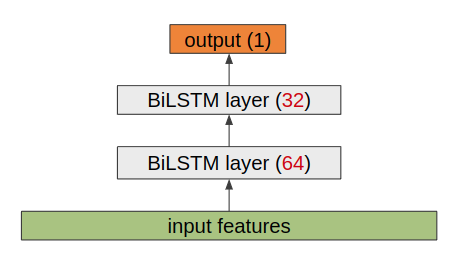
\includegraphics[width=8cm]{./Chapitre5/figures/biLSTM2.png}}
  \end{minipage}
  \begin{minipage}[b]{0.49\linewidth}
      \center
      \centerline{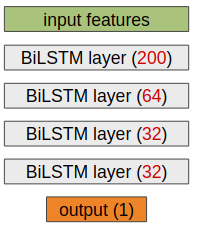
\includegraphics[width=8cm]{./Chapitre5/figures/biLSTM4.png}}
  \end{minipage}
    \caption{Schéma de la configuration des systèmes neuronaux appelés biLSTM-2 (à gauche) et biLSTM-4 (à droite). Le nombre de neurone est indiqué en rouge et entre paraenthèses sur chaque couche. Comme il s'agit de réseaux bidirectionnels, il faut multiplier par deux le nombre de neurones pour avoir le nombre de paramètres réels.}
    \label{fig:biLSTM}
\end{figure}


Les réseaux sont implémentés avec le framework Keras~\footnote{https://keras.io} en utilisant Tensorflow~\footnote{https://www.tensorflow.org/}. L'apprentissage se fait par lot de neuf conversations en utilisant l'optimiseur ADAgrad~\cite{Duchi2011} dont nous avons parlé au chapitre~\ref{chapitre2}. Les conversations sont mélangées entre chaque époque. Le learning rate est initialisé à 0,001.

Nous avons conservé les poids des réseaux donnant le meilleur score sur le développement afin de prédire les résultats sur le test.
Comme il s'agit d'une régression, le coefficient de corrélation de concordance (CCC)~\cite{CCC} a été utilisé comme fonction de coût pour l'apprentissage du réseau et comme métrique d'évaluation pour déterminer le meilleur système.
Pour rappel, ce score CCC varie de zéro (probabilité d'un tirage aléatoire) à un (corrélation parfaite).

\begin{table}[th]
  \centering
  \begin{tabular}{| l | ll | ll |}
      \hline
      Ensemble de descripteurs & \multicolumn{2}{c |}{\textbf{biLSTM-2}} &\multicolumn{2}{c |}{\textbf{biLSTM-4}} \\
      & dev & test & dev & test \\
      \hline
      eGeMAPS-88 &0.510 &0.363 &\textbf{0.666} &0.431 \\
      eGeMAPS-89 &\textbf{0.549} &\textbf{0.365} &0.619 &\textbf{0.542} \\
      f\_eGeMAPS-46 &0.469 &0.260 &0.607 &0.354 \\
      f\_eGeMAPS-47 &0.508 &0.359 &0.574 &0.422 \\
      \hline
  \end{tabular}
  \caption{Score CCC des systèmes de reconnaissance des émotions en utilisant quatre ensembles de descripteurs différents et deux architectures neuronales sur les ensembles de développement et de test d'AlloSat.}
  \label{tab:result7minutes}
\end{table}


Le tableau~\ref{tab:result7minutes} donne un résumé des résultats obtenus avec les modèles et les ensembles de descripteurs étudiés.
Nous pouvons remarquer que l'ensemble eGeMAPS-88 et 89 nous donne de meilleurs résultats sur les deux architectures neuronales que f\_eGeMAPS-46 et 47. Nous remarquons également que l'ajout d'un descripteur \textit{vad} permet de mieux généraliser puisque les scores sur le test sont toujours meilleurs lorsque l'on a ce descripteur. De plus, l'architecture qui donne les meilleurs résultats est biLSTM-4 quelque soit l'ensemble de descripteurs utilisé.

La meilleure configuration pour ce système de reconnaissance est donc le suivant :
\begin{itemize}
  \item Ensemble de descripteur eGeMAPS-89 (avec la vad),
  \item Architecture neuronale biLSTM-4 comportant quatre couches de biLSTM.
\end{itemize}

Ces premières expériences montrent que les réseaux neuronaux biLSTM sont capables de prédire les valeurs de l'axe de satisfaction et donc de retracer cette dimension au cours d’un appel avec un score CCC correct. Néanmoins le score CCC calculé sur l'ensemble des données doit être pris avec précaution car, comme nous le montrons dans la Figure~\ref{fig:result7minutes}, le système est capable de faire de bonnes prédictions (conversation C) mais aussi de mauvaises prédictions (conversation D).

\begin{figure}[thb]
  \centering
    \begin{minipage}[b]{0.49\linewidth}
        \center
        \centerline{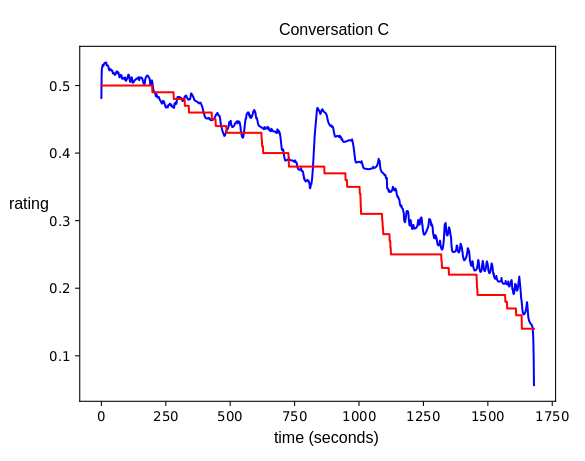
\includegraphics[width=8.4cm]{./Chapitre5/figures/test_ok.png}}
    \end{minipage}
    \begin{minipage}[b]{0.49\linewidth}
        \center
        \centerline{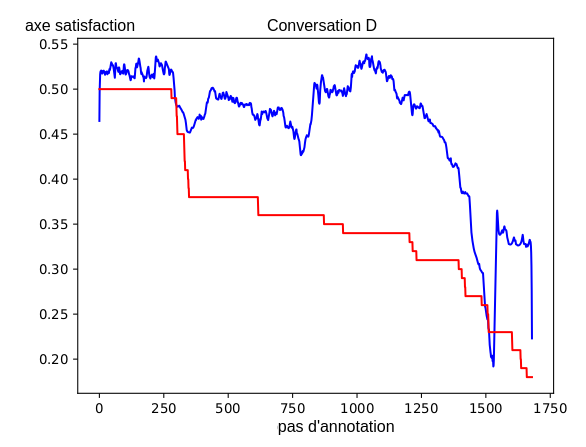
\includegraphics[width=8.4cm]{./Chapitre5/figures/test_not_ok.png}}
    \end{minipage}
    \caption{Prédiction de la satisfaction sur des conversations issues du test. La référence est en rouge, la prédiction en bleu.}
    \label{fig:result7minutes}
\end{figure}


\subsection{Décalage des annotations dans le temps}
Comme nous l'avons dit précédemment, il est tout à fait possible que les annotations soient décalées dans le temps. En effet, les annotateurs peuvent prendre plus ou moins de temps à annoter la variation d'une émotion. La question est assez complexe, puisque l'on ne connait pas la distribution des décalages. En effet, ils peuvent être très forts (décalage long) chez un annotateur ou dans une conversation en particulier, et très faible (décalage court) dans d'autres cas.

Néanmoins nous avons voulu savoir si en prenant en compte des décalages, nous sommes capables d'améliorer nos scores de reconnaissances des émotions.

Nous avons donc mis en place deux décalages : de deux secondes (soit huit pas d'annotations) et de quatre secondes (soit 16 pas d'annotations). Ce décalage à \textit{droite} consiste à décaler les annotations des segments émotionnels de $X$ pas d'annotations avec $X=8$ ou $X=16$. Les débuts de conversations, ainsi privés d'annotations, ont été remplacé par une annotation neutre de $0.50$. Les annotations \textit{trop à droite} ont été supprimées des données.

\begin{table}[h]
  \centering
\begin{tabular}{|l|l|l|l|l|l|l|}
\hline
Descripteurs & \multicolumn{2}{l|}{Sans décalage} & \multicolumn{2}{l|}{\begin{tabular}[c]{@{}l@{}}Décalage \\ 2 secondes\end{tabular}} & \multicolumn{2}{l|}{\begin{tabular}[c]{@{}l@{}}Décalage \\ 4 secondes\end{tabular}} \\ \hline
              & DEV             & TEST             & DEV                     & TEST           & DEV                     & TEST           \\ \hline
eGeMAPS\_88  & \textbf{0.666}   & \textbf{0.431}  & 0.603               & 0.293              & 0.489               & 0.230               \\ \hline
eGeMAPS\_89  & \textbf{0.619}   & \textbf{0.542}  & 0.601               & 0.303              & 0.502               & 0.278              \\ \hline
f\_eGeMAPS\_46  & \textbf{0.607}   & \textbf{0.354}  & 0.523               & 0.346              & 0.557               & 0.324              \\ \hline
f\_eGeMAPS\_47  & \textbf{0.574}   & \textbf{0.422}  & 0.477               & 0.245              & 0.450                & 0.231              \\ \hline
\end{tabular}
\caption{Score CCC des systèmes de reconnaissance des émotions d'une architecture neuronale bilstm à quatre couches en fonction du décalage des annotations.}
\label{tab:decalage}
\end{table}


Le tableau~\ref{tab:decalage} nous donne les résultats des systèmes utilisant l'architecture neuronale du biLSTM-4, présenté précédemment. Nous pouvons observer que quelque soit l'ensemble de descripteur utilisé, les scores sur les données de dev et de test sont toujours meilleurs sans décalage. Même si le décalage permet d'atteindre des scores sur l'ensemble de développement avoisinant ceux sans décalage, on remarque que le pouvoir de généralisation du modèle en pâtit grandement. Nous avons également essayer de plus forts décalages, à savoir huit et 12 secondes, mais les résultats ne font que se dégrader.

Pour notre corpus et en utilisant des architectures de type biLSTM, le décalage des annotations ne permet pas d'améliorer les scores de reconnaissance des émotions.

\subsection{Comparaison eGeMAPS et MFCC}
En reconnaissance des émotions, la plupart du temps, la représentation acoustique se concentre principalement sur la capture de la prosodie. C'est pour cette raison que les ensembles de descripteurs dits \textit{experts} sont majoritairement utilisés. En effet, comme nous l'avons dit précédemment dans le chapitre~\ref{chapitre3}, ces ensembles de descripteurs sont particulièrement adaptés dans le cadre de la recherche des émotions.

Cependant, dans notre contexte de capture des conversations, à savoir les conversations téléphoniques, le signal audio peut être plus ou moins dégradé et l'extraction de ces ensembles de descripteurs \textit{experts} peut contenir beaucoup d'erreurs. Les extracteurs ne sont, en général, pas prévus pour fonctionner avec des signaux dits dégradés.

Il peut donc être intéressant de comparer l'ensemble eGeMAPS à des descripteurs plus robustes aux signaux dégradés. Pour cela nous avons fait le choix de les comparer aux MFCC, que nous avons détaillé au chapitre~\ref{chapitre3}. Les MFCC sont plus robustes et leurs extracteurs sont plus fiables dans des contextes de signaux dégradés.

Nous avons décidé de comparer les MFCC issus de deux outils d'extraction différents : OpenSMILE dont nous avons déjà parlé et librosa\footnote{https://librosa.github.io/librosa/}. En effet, il est possible d'observer des variations entre plusieurs extracteurs~\cite{Ganchev2005}. Une fois ces extractions effectuées, nous avons mis en place deux protocoles pour les adapter à nos segments émotionnels de 250~ms :
\begin{itemize}
        \item \textbf{Mfcc-Os} correspond aux MFCC 1 à 13 ainsi qu'à leurs dérivés premières et secondes pour qualifier la dynamique du signal. Ces 39 descripteurs ont été extraits avec l’outil OpenSMILE. Pour se référer à un segment émotionnel, nous avons calculé la moyenne et l'écart type de ces descripteurs. Ainsi nous avons un ensemble de 78 descripteurs pour chaque segment émotionnel.
        \item \textbf{Mfcc-lib} correspond aux MFCC 1 à 24 qui sont extraits tous les 10~ms sur des fenêtres de 30~ms. Ces 24 descripteurs ont été extraits avec l'outil librosa. Comme pour les descripteurs précédents, nous avons calculé la moyenne et l'écart type de ces descripteurs au niveau du segment émotionnel. Ainsi nous avons un ensemble de 48 descripteurs pour chaque segment émotionnel.
    \end{itemize}

Nous utilisons la meilleure des deux architectures neuronales de la section précédente pour faire notre comparatif, à savoir le biLSTM-4 couches. Les résultats sont regroupés dans le tableau~\ref{tab:egemapsVSmfcc}.

\begin{table}[ht!]
    \centering
    \begin{tabular}{| l | l | l |}
    \hline
    \textbf{Features} &\multicolumn{2}{l|}{\textbf{AlloSat}} \\
    %\hline
    &DEV &TEST \\
    \hline
    eGeMAPS-88  &0.666  &0.431\\
    %eGeMAPS-89  &.619  &\textbf{.542}\\
    eGeMAPS-46  &0.607  &0.354\\
    %eGeMAPS-47  &.574  &.422\\
    Mfcc-lib 48    &\textbf{0.675}  &\textbf{0.510}\\
    Mfcc-Os 78    &0.382  &0.299\\
    \hline
\end{tabular}
    \caption{Comparaison de performance entre descripteurs experts et MFCC. Score CCC rapporté sur les différents ensembles de descripteurs sur le dev et le test d'AlloSat. Le modèle utilisé est le biLSTM-4.}
    \label{tab:egemapsVSmfcc}
\end{table}


Nous pouvons observer tout d'abord une forte différence de score entre les deux types de MFCC. Outre la différence d'implémentation de l'extraction, nous avons mis en place deux protocoles différents pour ces descripteurs, ce qui peut expliquer cette différence de score. On observe également que les Mfcc-lib ont une meilleure performance que l'ensemble eGeMAPS-89 sur le dev. Ce score semble confirmer que les MFCC sont plus adaptés au signal téléphonique, pour notre corpus, sur la tâche de reconnaissance des émotions.

\subsection{Comparaison CNN et biLSTM}
Dans les travaux menés par Schmitt et al.~\cite{Schmitt2019}, les architectures CNN et biLSTM sont comparées. Le postulat de ces travaux sont que nous avons trop tendance à complexifier nos architectures neuronales dans les expériences, et qu'à complexité égale, un système à base de CNN peut faire aussi bien voir mieux qu'un système à base de réseaux récurrents.

Nous avons donc voulu confronter leur conclusion à notre propre corpus, pour voir si nous pouvions améliorer nos résultats. En plus des deux architectures biLSTM précédemment expliqué, nous avons mis en place une architecture à base de quatres couches convolutionelles, avec une activation de type ReLU. Comme pour les autres systèmes, un unique neurone en sortie permet de faire la prédiction de la valeur de satisfaction. Le CNN est décrit dans la figure~\ref{fig:CNN}.

\begin{figure}[thb]
  \centering
    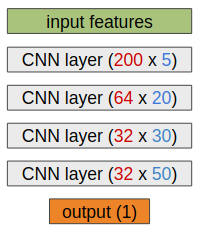
\includegraphics[width=5cm]{./Chapitre5/figures/CNN.png}
    \caption{Schéma de la configuration du système neuronal appelé CNN-4. Le nombre de neurons est en rouge et le filtre recepteur en bleu.}
    \label{fig:CNN}
\end{figure}


Afin de réaliser la comparaison, nous avons décidé de comparer nos résultats avec ceux des travaux réalisés sur le corpus SEWA. Pour cela, nous avons utilisé l'ensemble de descripteur eGeMAPS-47, utilisé par Schmitt et al.~\cite{Schmitt2019}. Nous avons donc refait leur expérimentation sur le corpus SEWA et nous l'avons adapté au corpus AlloSat, en partant du code du challenge AVEC disponible sur github\footnote{https://github.com/AudioVisualEmotionChallenge/AVEC2019}.

Nous avons eu quelques difficultés à faire converger le système convolutif sur nos données. Nous avons donc fait le choix de présenter dans le tableau~\ref{tab:cnnVSbilstm} la moyenne de cinq systèmes dont les poids ont été initialisés différemment (contrôlé par le paramètre \textit{seed}), ainsi que le meilleur des cinq systèmes sur l'ensemble de développement.

\begin{table}[h]
  \centering
\begin{tabular}{|l|l|l|c|c|c|}
\hline
\multirow{2}{*}{Modèles} & \multirow{2}{*}{Descripteurs} & AlloSat                               & \multicolumn{3}{c|}{SEWA}                                                                                             \\ \cline{3-6}
                         &                               & satisfaction                          & activation                            & valence                               & liking                                \\ \hline
\multicolumn{6}{|c|}{\textbf{Reproduction des résultats avec nos systèmes}}                                                                                                                                              \\ \hline
CNN                      & eGeMAPS-47                    & .178 (.458)                           & \textbf{.528} (.541) & \textbf{.515} (.527) & \textbf{.304} (.321) \\
biLSTM-4                 & eGeMAPS-47                    & \textbf{.437} (.458) & .487 (.527)                           & .428 (.468)                           & .258 (.346)                           \\ \hline
% \multicolumn{6}{|c|}{\textbf{Schmitt et al.~\cite{Schmitt2019} : Train et Dev sur les conversations allemandes}}                                                                                                           \\ \hline
% CNN                      & eGeMAPS-47                    &                                       & .571                                  & .517                                  &                                       \\
% biLSTM-4                 & eGeMAPS-47                    &                                       & .568                                  & .561                                  &                                       \\ \hline
\end{tabular}
\caption{Comparaison des moyennes des scores CCC de cinq systèmes différents sur l'ensemble de développement d'AlloSat et de SEWA.}
 %Nous avons également reporté les résultats issus de Schmitt et al.~\cite{Schmitt2019}}
\label{tab:cnnVSbilstm}
\end{table}


Comme nous pouvons l'observer, nous avons un grand écart entre la moyenne des scores et le score maximal pour le CNN sur le corpus AlloSat. En effet, sur les cinq systèmes, seuls deux ont finis par converger. De plus, nous n'avons pas réussi à reproduire parfaitement les scores sur le corpus SEWA. L'initialisation des systèmes joue un très grand rôle dans le score final. On remarque également que les scores atteints avec une architecture biLSTM-4 sur l'axe de satisfaction est comparable aux scores obtenus sur les axes d'activation et de valence de SEWA.

Pour conclure, nous avons montré que les systèmes à base de couches convolutives ne sont pas compatibles avec notre corpus. De plus, nous voulons à terme travailler sur des séquences de taille non fixe, ce qui ne peut pas être réalisé avec des CNN.

\section{En utilisant l'intégralité des conversations}
D'après ce que nous avons observé sur les extraits de conversations, nous avons décidé de faire des expérimentations sur la totalité des conversations en utilisant les différentes configurations expliquées plus tôt. Nous ne pouvons pas faire d'expérimentations à partir de systèmes à base de CNN, dû à la nature de ce réseau, qui permet de faire des reconnaissances à partir de séquences de taille fixe.

Nous avons également choisi de changer d'implémentation en passant de l'utilisation de Keras à celle de Pytorch~\cite{pytorch}. En effet cet outil permet de gérer plus en profondeur les paramètres des réseaux et a un temps d'apprentissage fortement diminué.

\subsection{Changer de fonction de coût}
Comme nous l'avons vu précédemment dans le chapitre~\ref{chapitre3}, le Coefficient de Corrélation de Concordance est un outil d'évaluation très utilisé dans la reconnaissance d'émotions continues. Les challenges AVEC~\cite{AVEC2018} ont notamment contribué à la standardisation de l'utilisation de cette métrique pour évaluer les systèmes de reconnaissance d'émotion continue. Pour rappel, le CCC se calcule selon l'équation~\ref{eq:CCCscore}.

\begin{equation}
   \rho = \frac{2\rho\sigma_x\sigma_y}{\sigma_x^2 + \sigma_y^2 + (\mu_x - \mu_y)^2}
\label{eq:CCCscore}
\end{equation}

Si on regarde l'équation, quand la référence est constante sur la conversation totale, $\sigma_y = 0$ et donc le coefficient est égal à zéro. De façon plus général, quand la référence varie peu, le CCC va s'approcher de zéro, même si la prédiction est quasiment parfaitement synchronisée à la référence.

On peut donc en conclure que la fonction de coût va pénaliser les conversations où la référence varie peu ($\sigma_y \simeq 0$) et que le système ainsi entraîné aura du mal à prédire correctement de tels références.

\begin{table}[htp]
\centering
\begin{tabular}{| l | l l |}
    \hline
    \textbf{Descripteurs} &\multicolumn{2}{c|}{\textbf{AlloSat}} \\
      &\textit{l-ccc}   &\textit{l-rmse}  \\
    \hline
    eGeMAPS-47  &.437 &.381       \\
    eGeMAPS-88  &.564 &.514       \\
    Mfcc-lib    &.675  &\textbf{.698} \\
    Mfcc-Os     &.382   &405      \\
    \hline
\end{tabular}
\caption{Score CCC des systèmes de reconnaissance des émotions sur l'ensemble de développement d'AlloSat. On compare l'utilisation de deux fonctions de coût \textit{l-ccc} et \textit{l-rmse}. Les systèmes sont issus de l'architecture neuronale biLSTM-4.}
\label{tab:cccVSrmse}
\end{table}


Nous avons comparé les scores obtenus en utilisant la RMSE comme fonction de coût que nous avons introduit au chapitre~\ref{chapitre3} pour palier à ce problème. Le tableau~\ref{tab:cccVSrmse} résume les différences de scores calculés sur le dev.

Comme nous pouvons l'observer, les scores sont majoritairement meilleurs si on utilise la fonction de coût CCC. On remarque cependant que dans le cas des descripteurs \textit{Mfcc-lib}, l'utilisation de la fonction de coût RMSE permet d'améliorer les résultats. Cependant lorsque l'on regarde la prédiction effective sur les conversations, on se rend compte que les prédictions ne sont pas homogènes en terme de qualité, comme en témoigne la figure~\ref{fig:cccVSrmse}.

\begin{figure}[h]
        \centering
        \begin{subfigure}{.49\textwidth}
          \centering
          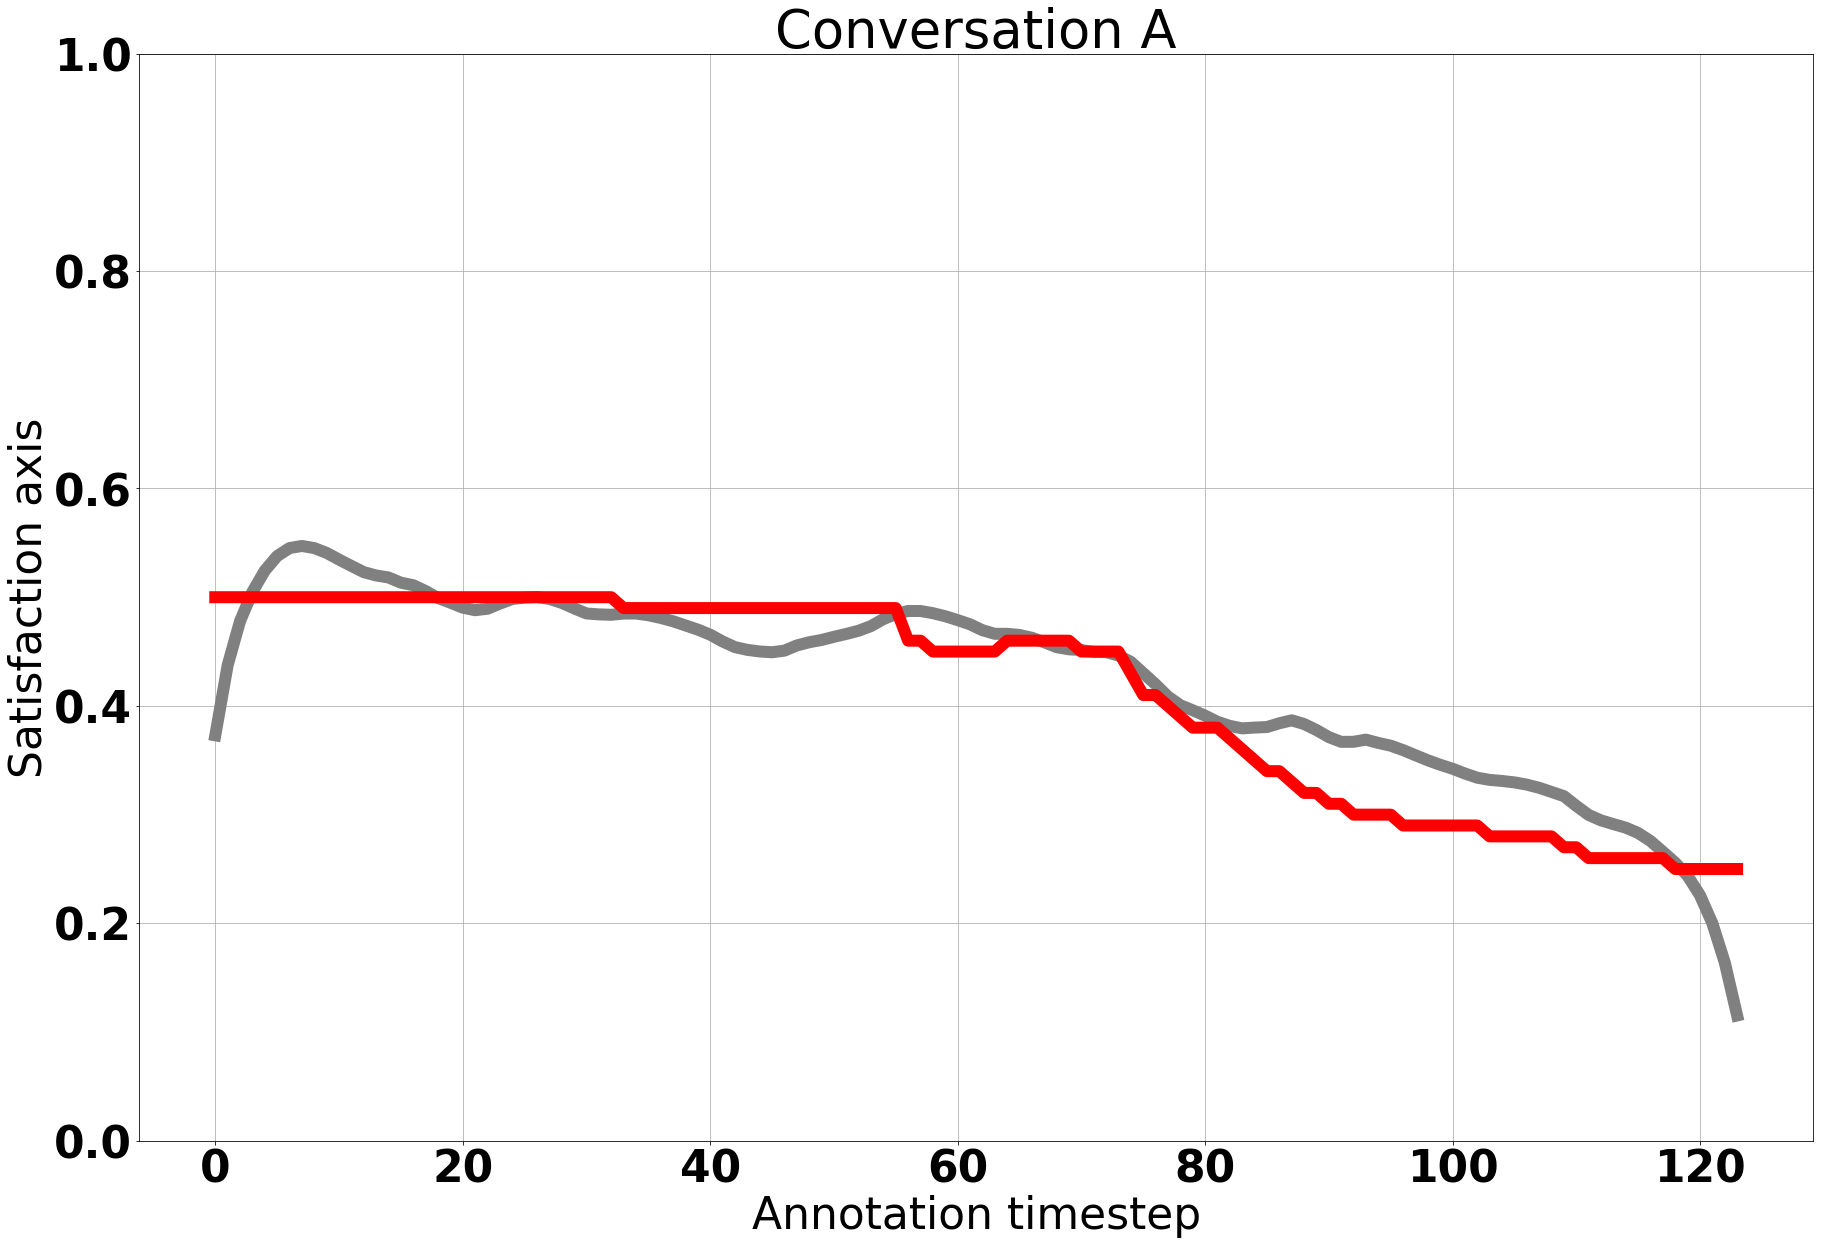
\includegraphics[width=.99\linewidth]{./Chapitre5/figures/cccVSrmse1.png}
        \end{subfigure}
        \begin{subfigure}{.49\textwidth}
          \centering
          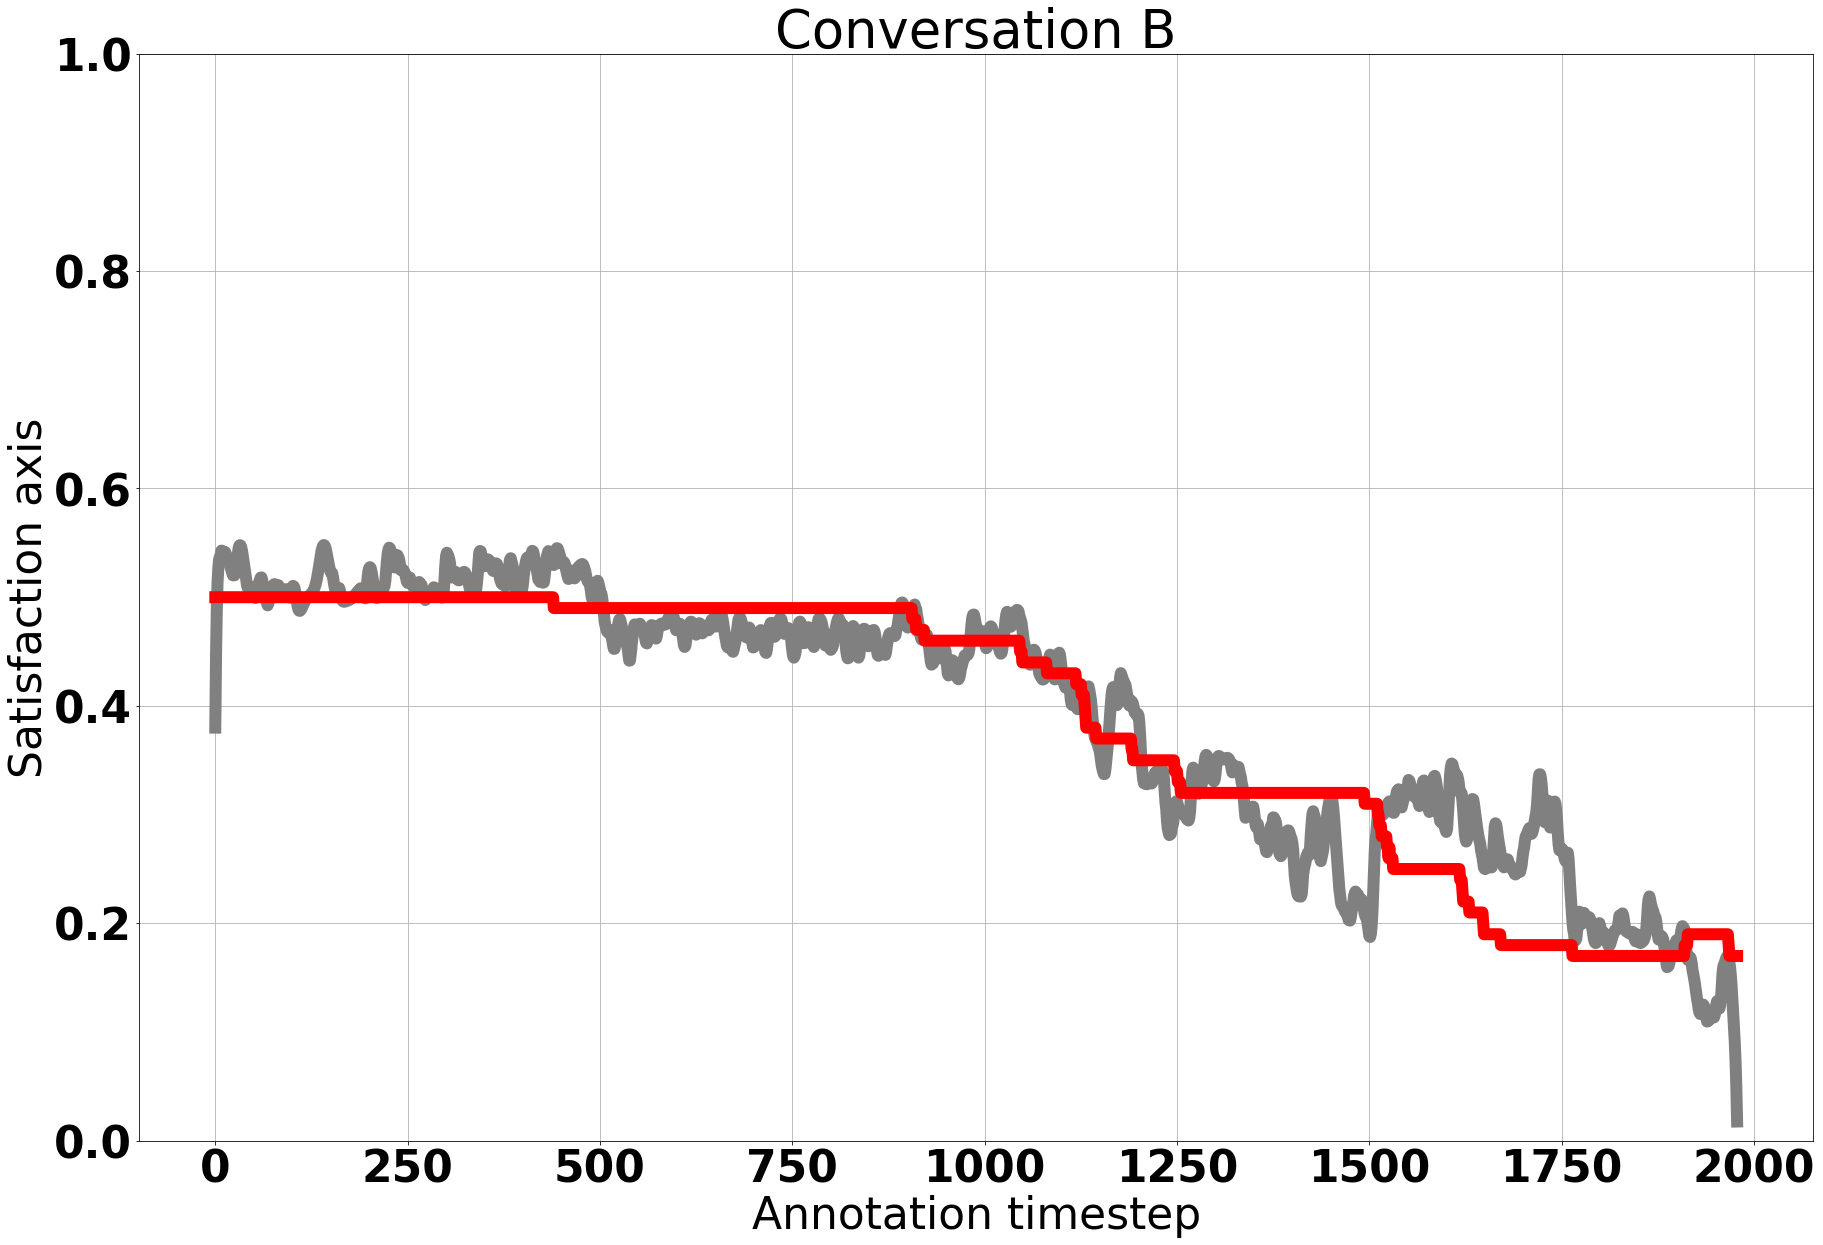
\includegraphics[width=.99\linewidth]{./Chapitre5/figures/cccVSrmse2.png}
        \end{subfigure}
        \caption{Evolution des prédictions (grises) et des références (rouge) de deux conversations provenant de l'ensemble de test d'AlloSat. $ccc(A) = 0.564$, $ccc(B) = 0.903$.}
        \label{fig:cccVSrmse}
    \end{figure}


Nous avons donc décidé de mettre en place un post-traitement afin de lisser les courbes de prédiction, pour avoir une meilleure représentation des émotions.

\subsection{Post-traitement : lissage des prédictions}
Nous avons décidé de mettre en place un lissage des prédictions. Pour cela, nous avons utilisé l'algorithme de lissage Savistky-Golay~\cite{Savitzky1964} avec un degré polynomial de zéro. Bien qu'ancien, cet algorithme est toujours autant utilisé dans la gestion des signaux. C'est une extension de la moyenne glissante, qui est utilisée pour atténuer les pics des signaux en approximant un polynôme pour chaque fenêtre de la moyenne glissante, ici un polynôme de degré zéro. Nous avons fait le choix de ce degré puisque c'est celui qui va lisser au maximum la courbe.
%It has been applied to the series of data with a window of 101, again, to try flatten the curve as much as possible.

Nous avons donc appliqué ce lissage sur les prédiction du meilleur système obtenu jusque là, les résultats sont disponibles dans le tableau~\ref{tab:lissage}.


\begin{table}[h]
    \centering
        \begin{tabular}{| l | l l | l l |}
        \hline
        \textbf{Descripteurs} &\multicolumn{2}{c|}{\textbf{Dev}}& \multicolumn{2}{c |}{\textbf{Test}}\\
        &Non lissé &Lissé &Non lissé &Lissé \\
        \hline
        Mfcc-lib (\textit{l-rmse})    &.698 &\textbf{.719} &.513 &\textbf{.570}  \\
        \hline
    \end{tabular}
    \caption{Scores CCC avec et sans lissage calculés sur les ensembles de développement et de test d'AlloSat. Score issu du meilleur modèle : système biLSTM-4, descripteurs Mfcc-lib et fonction de coût RMSE.}
    \label{tab:lissage}
\end{table}


Nous pouvons observer qu'il s'agit du meilleur score jamais obtenu sur les prédictions de l'axe de satisfaction. De même, la figure~\ref{fig:lissage} permet de se rendre compte du profit que nous tirons du lissage.

\begin{figure}[h]
    \centering
    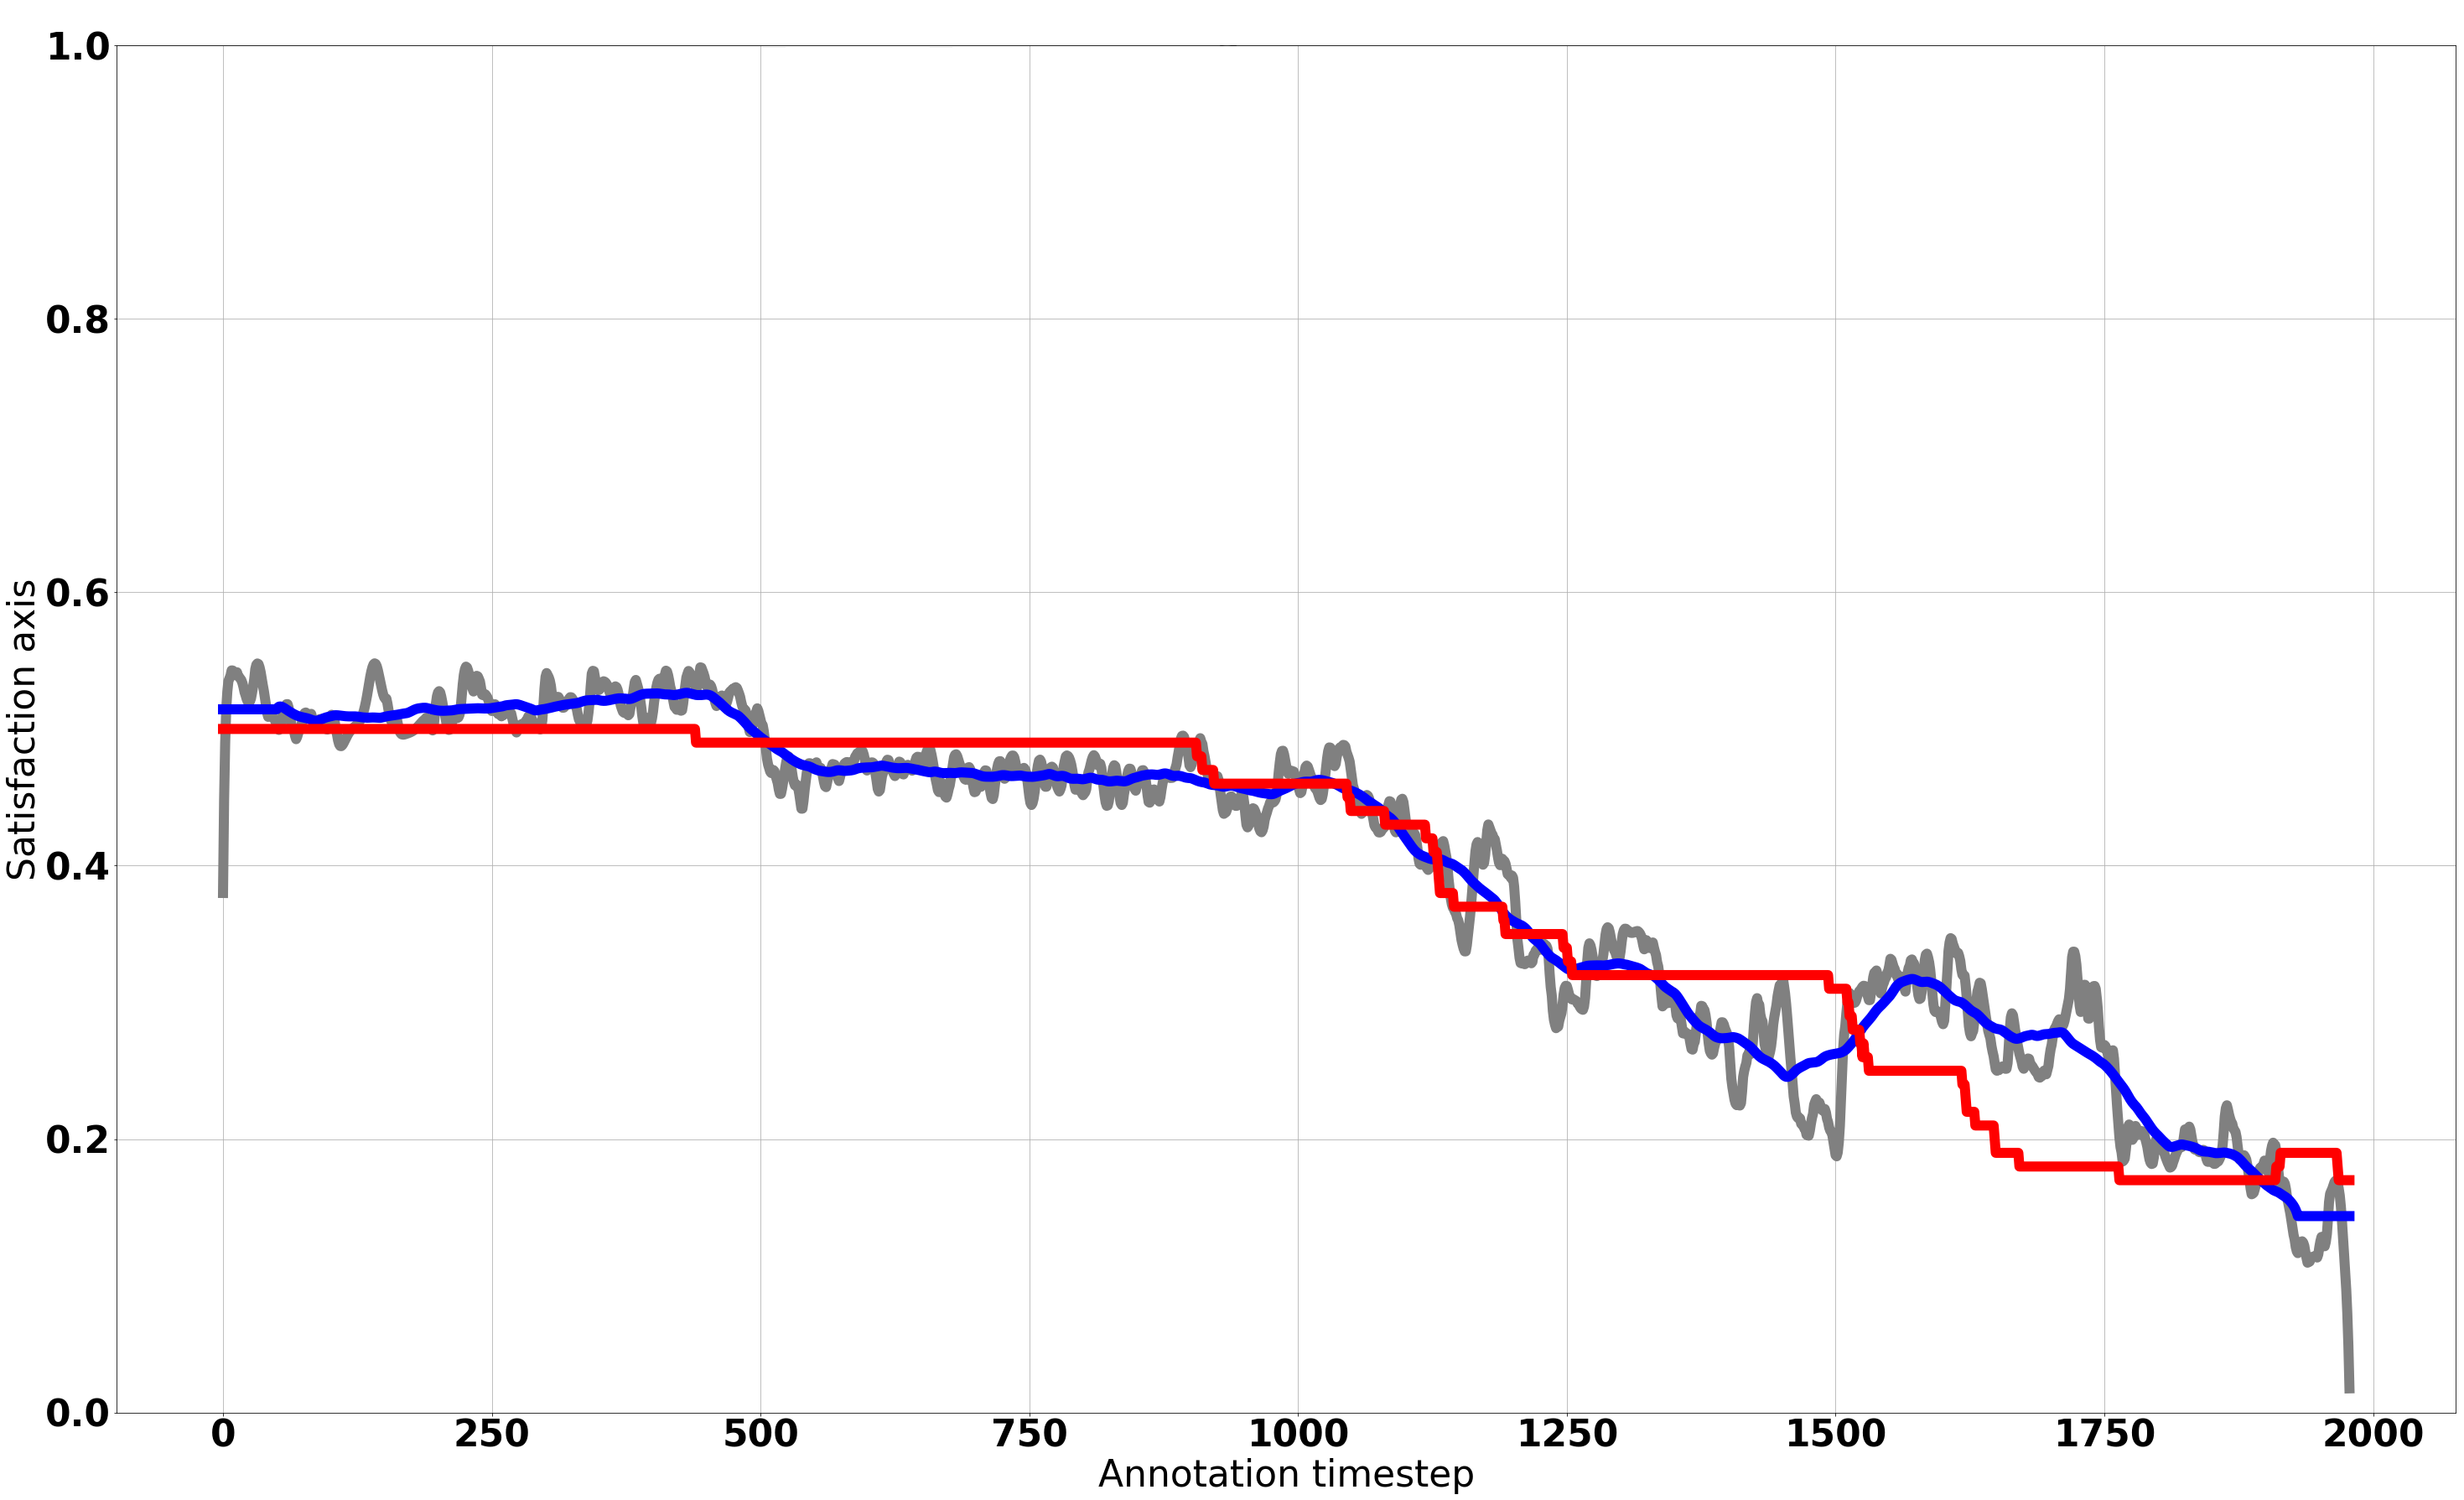
\includegraphics[width=.99\linewidth]{./Chapitre5/figures/lissage2.png}
    % \begin{subfigure}{.49\textwidth}
    %   \centering
    %   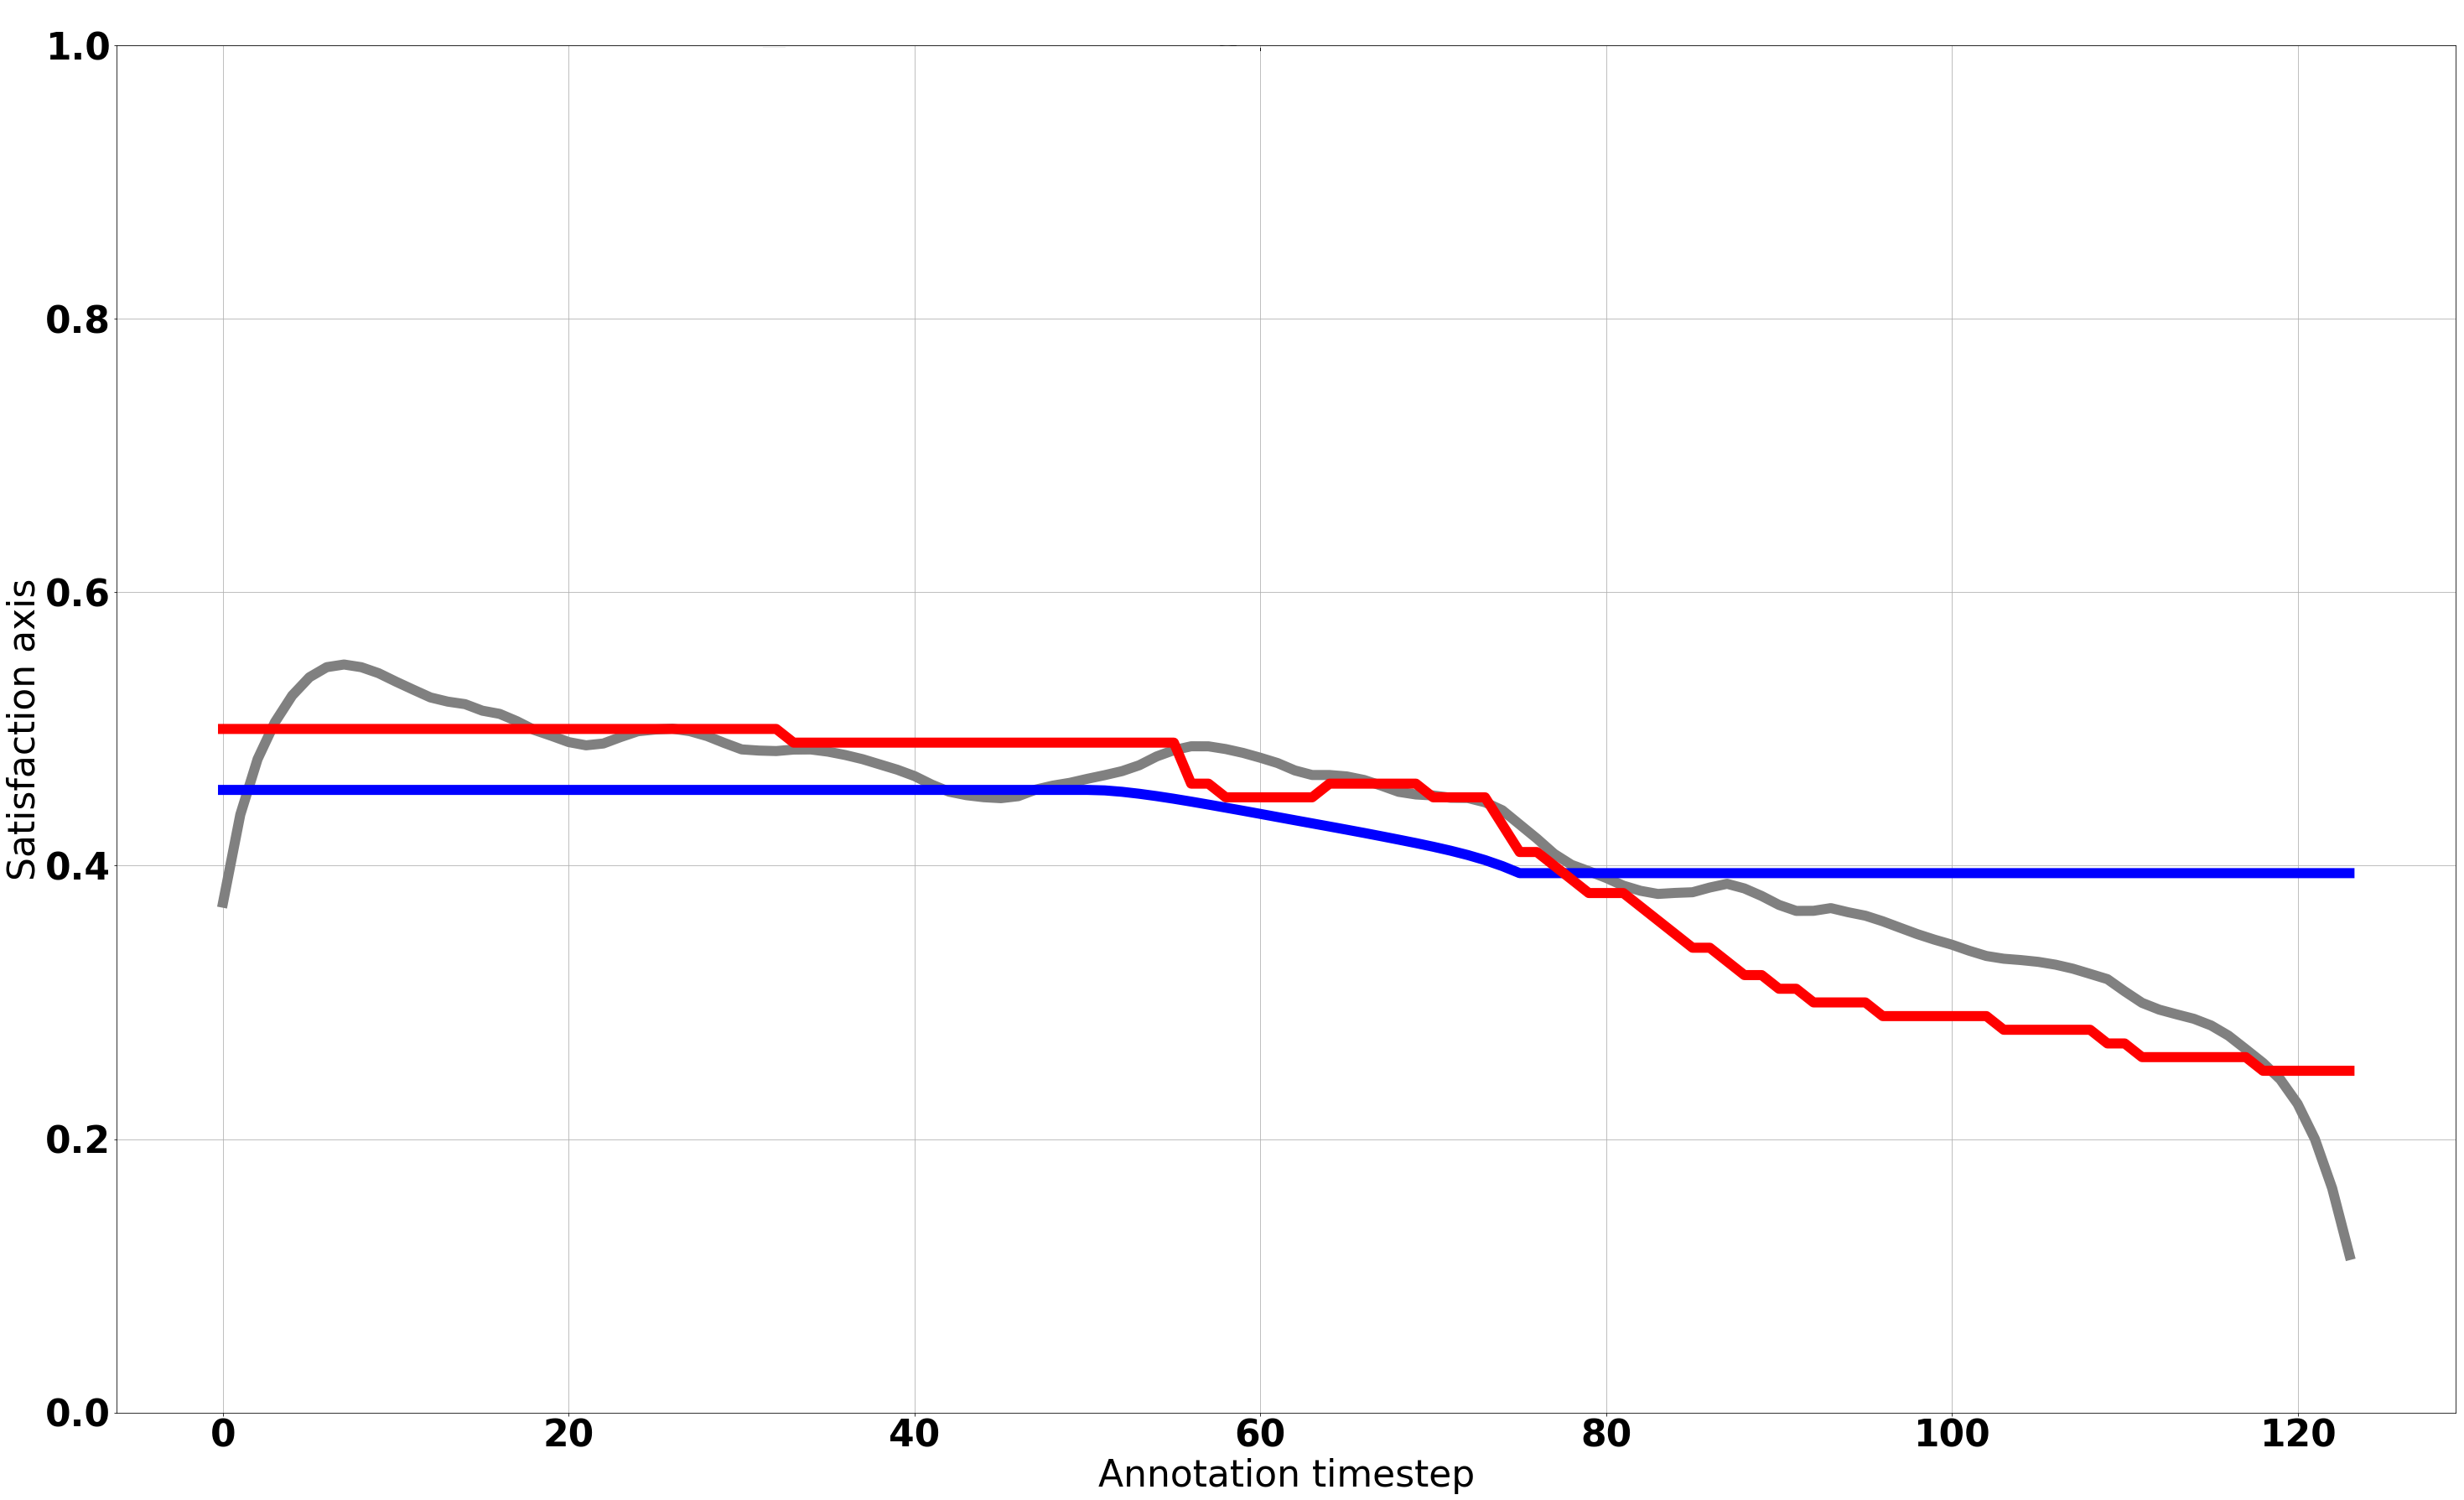
\includegraphics[width=.99\linewidth]{./Chapitre5/figures/lissage1.png}
    % \end{subfigure}
    % \begin{subfigure}{.49\textwidth}
    %   \centering
    %   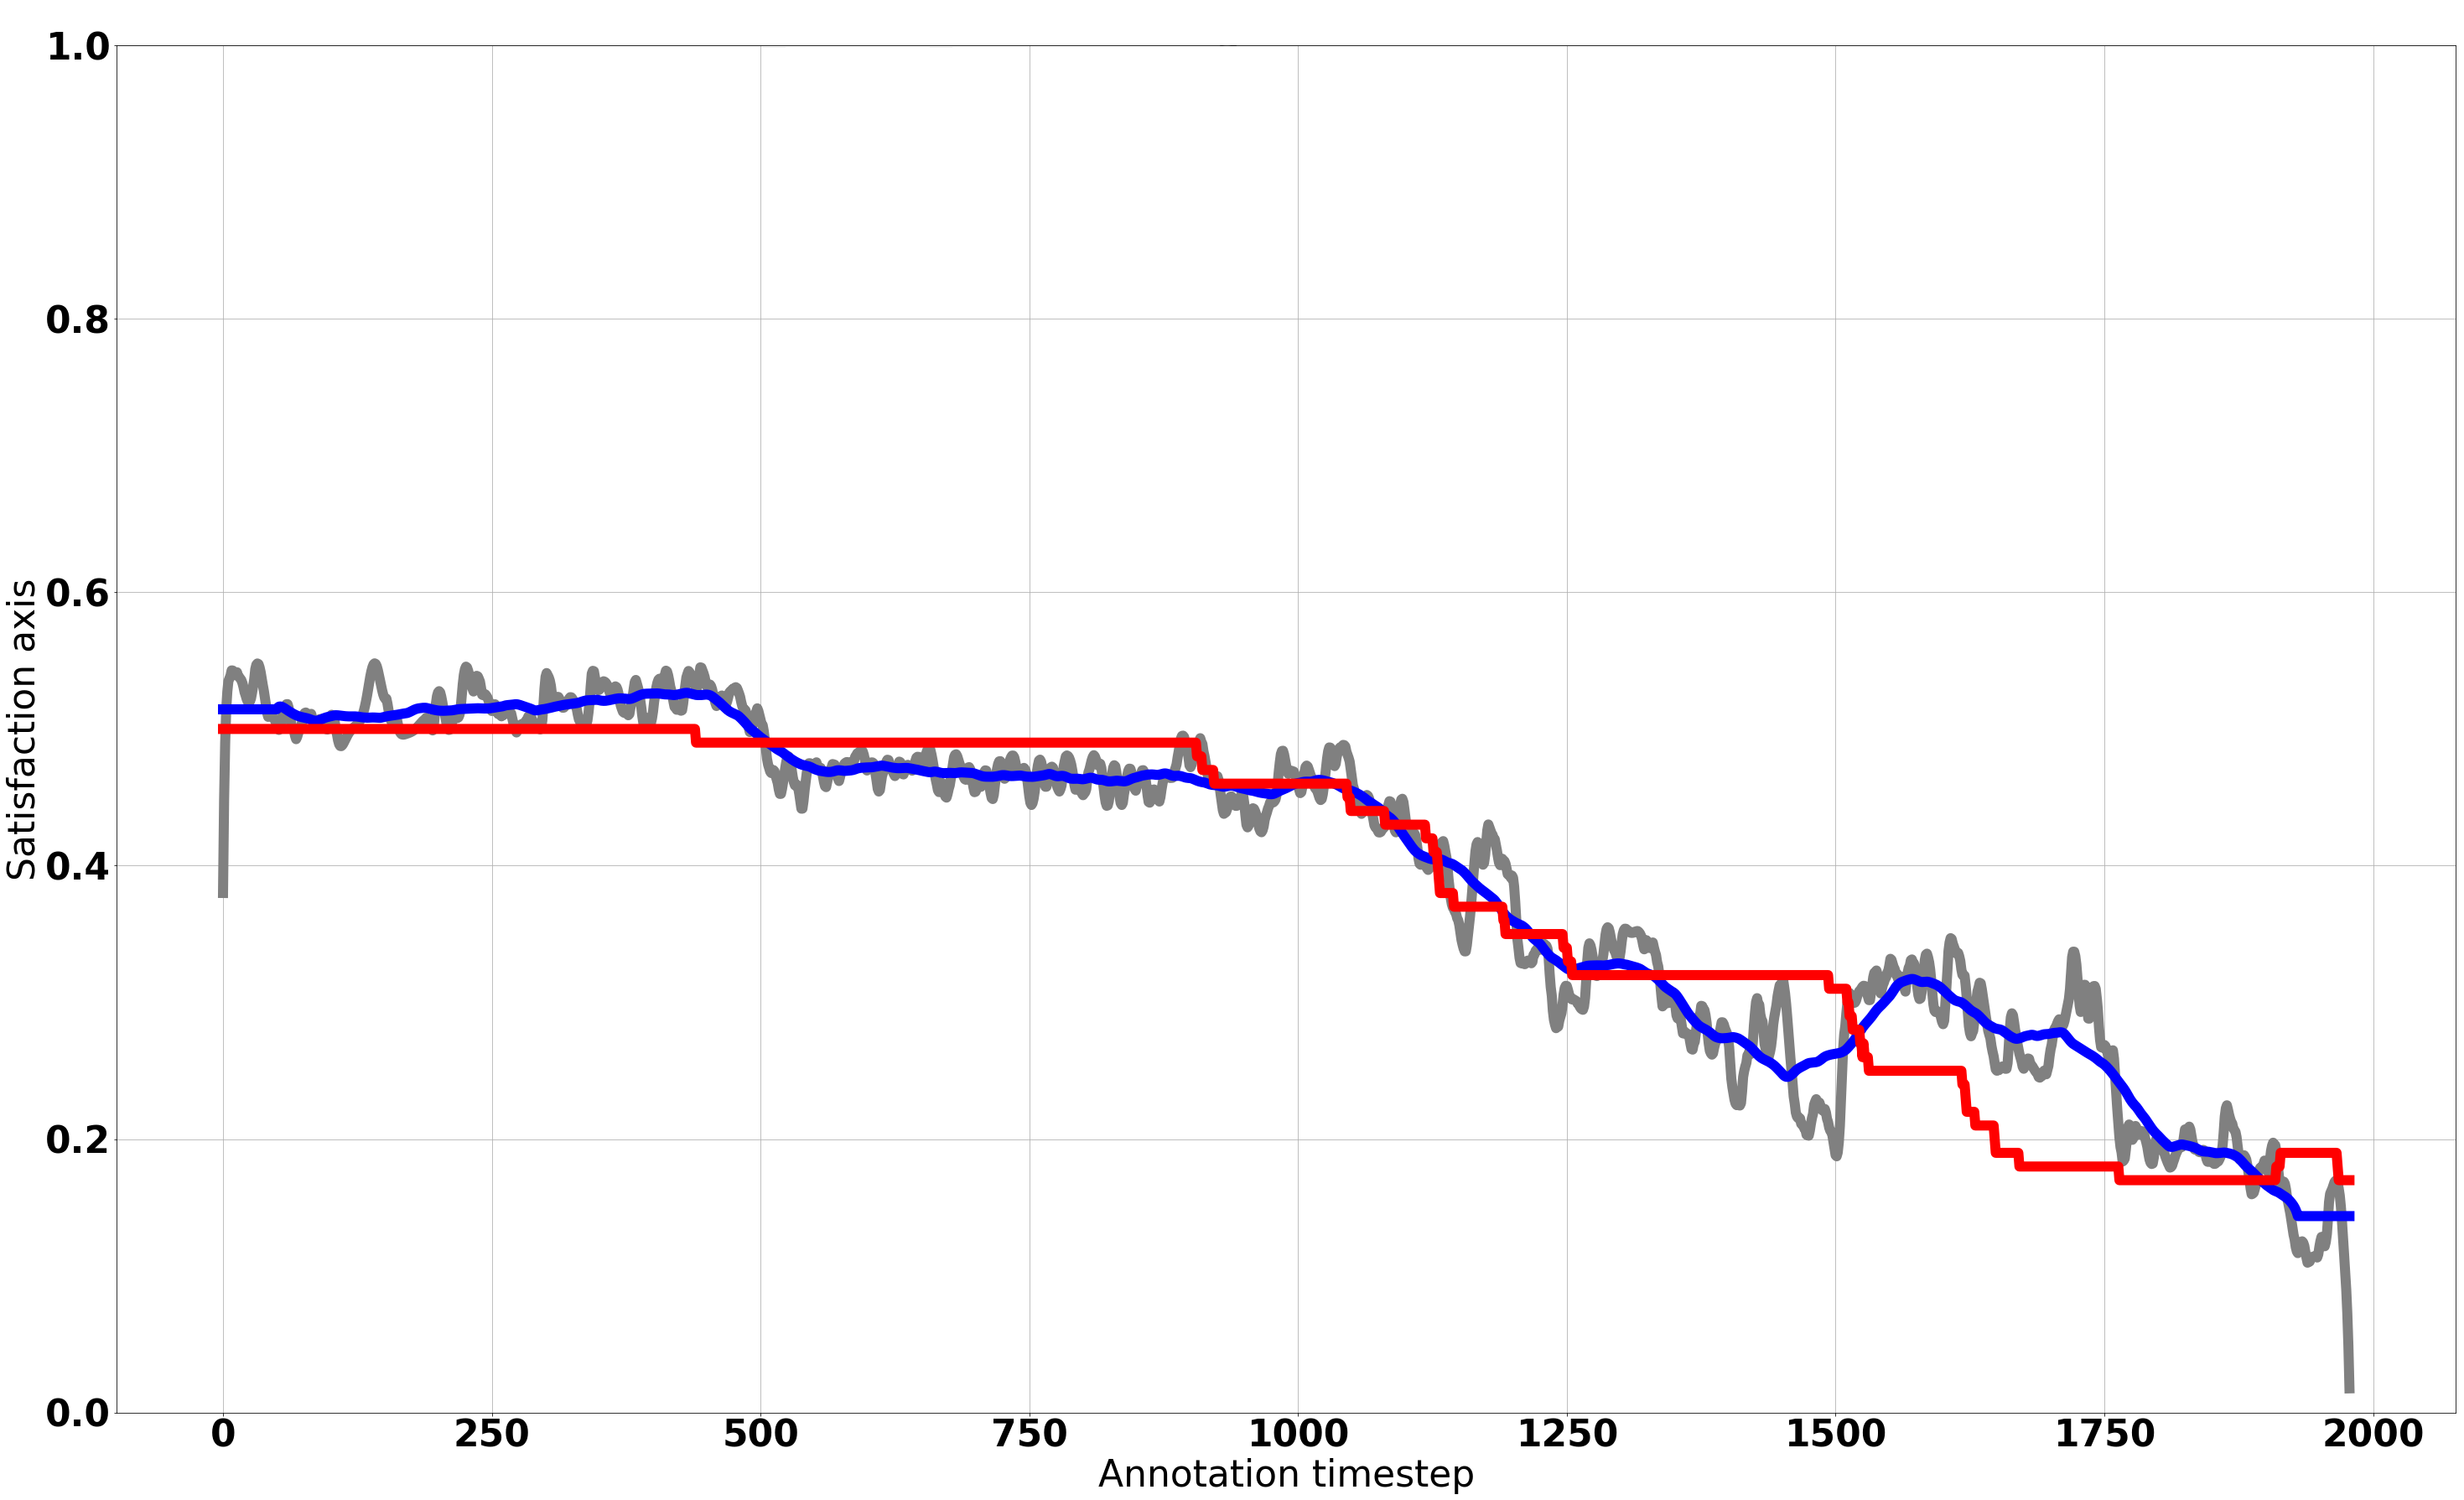
\includegraphics[width=.99\linewidth]{./Chapitre5/figures/lissage2.png}
    % \end{subfigure}
    \caption{Comparaison entre les prédictions lissées et non lissées d'une conversation de l'ensemble de test d'AlloSat. La référence est en rouge, les prédictions en gris et les prédictions lissés en bleu.}
    \label{fig:lissage}
\end{figure}


Grâce à ce lissage, nous obtenons de très bons scores : $0.719$ pour l'ensemble de développement et $0.570$ pour le test. Nous avons voulu confronter ces scores à ceux obtenus dans l'état de l'art, sur le corpus SEWA.

\subsection{Comparaison avec SEWA}
Pour comparer nos résultats avec ceux obtenus sur le corpus SEWA, nous nous sommes remis dans les conditions d'expérimentation des campagnes AVEC 2018 et 2019. Nous avons également comparés nos résultats avec ceux obtenus par Schmitt et al.

Tout d'abord nous avons repris les systèmes décrits dans ces expérimentations pour reproduire les résultats reportés dans les différents articles:

\begin{itemize}
  \item biLSTM-2 : comme montré dans la figure~\ref{fig:biLSTM}, il s'agit d'un système à deux couches de biLSTM de 64 et 32 neurones. Un seul neurone est utilisé pour la sortie. Ce système est utilisé comme baseline dans les campagnes AVEC~\cite{AVEC2018,AVEC2019} en 2018 et 2019 pour la sous-catégorie \textit{cross-cultural affect}. Il est constitué de 337 473 paramètres.
  \item biLSTM-4 : comme montré dans la figure~\ref{fig:biLSTM}, il s'agit d'un système à quatre couches de biLSTM de 200, 64, 32 et 32 neurones. Un seul neurone est utilisé pour la sortie. Ce système est utilisé dans les travaux de Schmitt et al.~\cite{Schmitt2019}. Il est constitué de 702 593 paramètres.
\end{itemize}

\begin{table}[ht!]
      \centering
      \begin{tabular}{| l| l |l |c | c | c |}
          \hline
          \textbf{Modèles} &\textbf{Descripteurs} &\textbf{AlloSat-Dev} &\multicolumn{3}{c |}{\textbf{SEWA-Dev}} \\ \cline{3-6}
          & &satisfaction &activation &valence &liking \\
          \hline
          \multicolumn{6}{| c |}{Nos systèmes : pour SEWA Train et Dev sur les conversations allemandes} \\
          \hline
           \rowcolor{Red}
           CNN       &eGeMAPS-47 &.178 (.458) &\textbf{.528} (.541) &\textbf{.515} (.527) &\textbf{.304} (.321)  \\
            \rowcolor{Red}
           biLSTM-4  &eGeMAPS-47 &.437 (.458) &.487 (.527) &.428 (.468) &.258 (.346)  \\
          \rowcolor{Green}
          biLSTM-2 &eGeMAPS-88  &.480 (.564) &.280 (.357) &.174 (.212) &.095 (.171) \\
          \rowcolor{Green}
          biLSTM-2 &Mfcc-Os     &.364 (.439) &.395 (.438) &.325 (.373) &.158 (.208) \\
           \rowcolor{Blue}
          biLSTM-2 &eGeMAPS-88*  &.480 (.564) &.244 (.273) &.118 (.155) &.082 (.132) \\
          \rowcolor{Blue}
          biLSTM-2 &Mfcc-Os*     &.364 (.439) &.325 (.326) &.186 (.192) &.125 (.126) \\
          biLSTM-4 &eGeMAPS-88  &.564 (.634) &.316 (.429)  &.237 (.309) &.119 (.188) \\
          biLSTM-4 &Mfcc-lib    &\textbf{.666} (.675) &.489 (.501) &.449 (.464) &.124 (133) \\
          biLSTM-4 &Mfcc-Os &.374 (.382) &- &- &- \\
          \hline
          \multicolumn{6}{| c |}{AVEC 2018 : Train et Dev sur les conversations allemandes~\cite{AVEC2018}} \\
          \hline
          \rowcolor{Green}
          biLSTM-2 &eGeMAPS-88 & &(.124)  &(.112) &(.001) \\
          \rowcolor{Green}
          biLSTM-2 &Mfcc-Os    & &(.253)  &(.217) &(.136) \\
           \hline
          \multicolumn{6}{| c |}{AVEC 2019 : Train et Dev sur les conversations allemandes et hongroises~\cite{AVEC2019}} \\
          \hline
          \rowcolor{Blue}
          biLSTM-2 &eGeMAPS-88* & &(.371) &(.286) &(.159) \\
          \rowcolor{Blue}
          biLSTM-2 &Mfcc-Os*    & &(.326) &(.187) &(.144) \\
           \hline
           \multicolumn{6}{| c |}{Schmitt et al. : Train et Dev sur les conversations allemandes~\cite{Schmitt2019}} \\
           \hline
           \rowcolor{Red}
           CNN      &eGeMAPS-47   & &(.571)  &(.517) & \\
           \rowcolor{Red}
           biLSTM-4 &eGeMAPS-47   & &(.568)  &(.561) & \\
           \hline
      \end{tabular}
      \caption{Comparaison des scores moyens de CCC sur les corpus AlloSat et SEWA selon quatre dimensions émotionnelles : la satisfaction, l'activation, la valence et le liking. Nos scores correspondent à la moyenne des scores de 5 systèmes appris avec des initialisations aléatoires différentes et entre parenthèses nous retrouvons le score du meilleur des modèles. Nous reportons également les résultats inclus dans les papiers~\cite{AVEC2018,AVEC2019,Schmitt2019}, qui constituent notre base de comparaison. Ces scores correspondent au meilleur de leur expérimentation, c'est pour cela qu'ils sont notés entre parenthèses, puisqu'à comparer avec les scores des meilleurs modèles notés entre parenthèses dans nos résultats.
      *L'entrainement et les prédictions sont réalisés sur les conversations allemandes et hongroises. Sans le sigle, l'entrainement et les prédictions sont réalisés sur les conversations allemandes uniquement.
      Les couleurs permettent de repérer les différentes expérimentations comparables.}
      \label{tab:allosatVSsewa}
  \end{table}


Les résultats sont disponibles dans le tableau~\ref{tab:allosatVSsewa}. L'initialisation étant un facteur important dans le score final des systèmes, nous avons fait le choix de présenter à la fois la moyenne de cinq systèmes initialisés aléatoirement et le meilleur de ces cinq systèmes. Comme nous pouvons l'observer, les résultats de nos modèles sont comparables à ceux obtenus dans les différentes baselines sur le corpus SEWA. Ils sont meilleurs que ceux diffusés lors de la campagne de 2018 mais moins performant que ceux de la campagne 2019. Les auteurs de la campagne ont eux-même reconnus que des variations de scores peuvent être observées en fonction de l'initialisation.

On remarque également que nous n'avons pas réussi à bien reproduire les résultats obtenus par Schmitt et al. sur l'activation et la valence. Ceci peut être dû notamment à l'initialisation mais également à la gestion du délai des annotations qui n'est pas pris en compte dans nos expérimentations. Nos systèmes sont plus performants sur la dimension du \textit{liking}, quelque soit les architectures utilisées.

Nous observons également, en comparant les meilleures performances et les performances moyennes, que le système biLSTM-2 entraîné avec les descripteurs Mfcc-Os sur les conversations allemandes et hongroises (en violet) semble être le moins sensible à l'initialisation des poids. De façon général, la plus grande disparité est observée sur la dimension du \textit{liking}.

Les performances obtenues sur l'axe de satisfaction sont comparables à celles obtenues sur les autres dimensions dans le cas de systèmes à base de réseaux récurrents. Les réseaux convolutifs, comme nous l'avons énoncé auparavant, ne semblent pas convenir à notre corpus. La prédiction de l'axe de satisfaction est plus performante avec des réseaux récurrents que des réseaux convolutifs. Il est donc plus prudent d'utiliser des réseaux récurrents lors de tâches de SER, puisqu'ils semblent plus robustes aux changements d'axe d'émotion et aux changements de corpus. De plus, la convergence des systèmes convolutifs n'est pas assurée en fonction des différents paramètres et hyper-paramètres du système.

En se concentrant sur la prédiction de l'axe de satisfaction, eGeMAPS-88 ($ccc=0.480$) semble mieux fonctionner que Mfcc-Os ($ccc=0.364$) avec le système biLSTM-2. Cependant, en utilisant le système biLSTM-4, les descripteurs eGeMAPS-47 atteignent également de bons résultats ($ccc=0.437$). Pour conclure sur le meilleur nombre de couches, nous effectuons une dernière expérience avec le système biLSTM-4 et eGeMAPS-88 ($ccc=0.564$) qui obtient notre meilleur résultat. Cette architecture semble être la plus convenable pour l'axe de satisfaction.

De cette expérience, nous concluons que le système biLSTM-4 est la meilleure des trois architectures comparées en ce qui concerne la robustesse à la variabilité induite par l'utilisation de différents corpus d'émotions et d'axe d'émotions. Nous cherchons les différences entre les deux corpus qui pourraient expliquer la différence de performance entre les systèmes sur ces deux corpus.

\subsection{Analyse des différences entre SEWA et AlloSat}

\subsubsection{Variation de l'annotation : pas de l'annotation, taux d'échantillonnage}
Nos premières hypothèses ont porté sur la durée du pas d'annotation et sur la différence de taux d'échantillonnage entre les deux corpus. Nous avons donc décidé de changer les pas d'annotation des deux corpus pour qu'ils soient comparables. Comme nous avons un corpus annoté toutes les 100~ms et l'autre annoté toutes les 250~ms, nous avons choisi de considérer l'annotation toutes les 500~ms. Pour cela, nous avons utilisé une moyenne glissante, afin de rester cohérent avec les annotations d'origines. Nous avons dans le même temps sur-échantillonné les conversations issues d'AlloSat, afin de se ramener à deux corpus échantillonnés selon le même taux soit 44kHz.

\begin{table}[htp!]
    \centering
    \begin{tabular}{|l|l||l|l|l|}
        \hline
                    &satisfaction &activation &valence &liking \\
        \hline
        CNN         &.046 (.151)   &.368 (.401) &.375 (.424) &.074 (.089)\\
        biLSTM-4    &.503 (.517)   &.457(.476) &.411(.420) &.248(.267) \\
        \hline
    \end{tabular}
    \caption{Comparaison entre les scores obtenus sur l'ensemble de développement d'AlloSat et de SEWA en prenant en entrée des segments émotionnels de 500~ms. Comparaison réalisé sur deux architectures neuronales : CNN et biLSTM-4.}
    \label{tab:pasAnnotation}
\end{table}


Les résultats, présentés sur le tableau~\ref{tab:pasAnnotation} ne permettent pas de valider ces deux hypothèses. En effet, les résultats sont comparables aux précédents.

\subsubsection{Variation de l'annotation : intensité de la dynamique}
En comparant les deux corpus, nous remarquons que l'axe de satisfaction varie très lentement dans le temps par rapport à l'activation et à la valence. Cela peut être dû au protocole d'annotation (la souris ou le joystick) et au contenu affectif annoté. Cette différence de variation peut être observée sur la figure~\ref{fig:variationAnnot} où la dynamique a été quantifiée en utilisant la ZCR sur les deltas des dimensions. Cette différence de variation pourrait expliquer la différence d'échelle entre les scores obtenus sur le corpus AlloSat et le corpus SEWA.

\begin{figure}[thb]
  \centering
    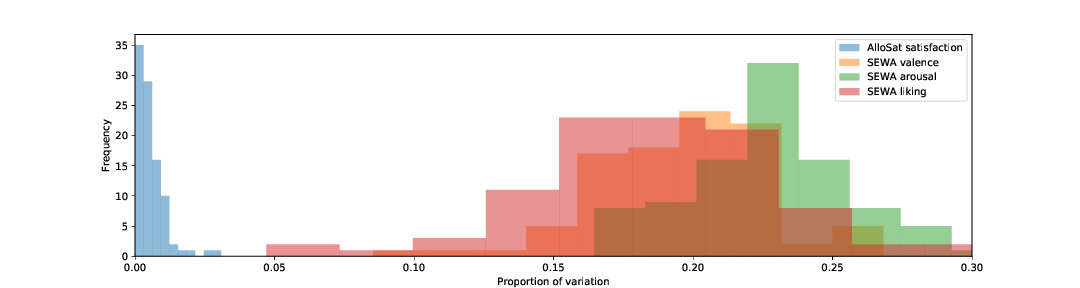
\includegraphics[width=18cm]{./Chapitre5/figures/variation.jpeg}
    \caption{Fréquence des variations dans les annotations des corpus AlloSat et SEWA et leur intensité. La moyenne du nombre de variation de chaque axe dimensionnel est représenté en ordonnée et l'ordre de grandeur de ces variations est donné en abscisse.}
    \label{fig:variationAnnot}
\end{figure}


Pour déterminer si la dynamique dans l'annotation est responsable des mauvais résultats des systèmes convolutifs sur la satisfaction, nous effectuons des expériences supplémentaires avec des références lissées pour l'activation et la valence. Pour mettre en place le lissage, nous avons utilisé une moyenne glissante sur des fenêtres de 200, 500~ms et une seconde sur SEWA, ainsi que de 500~ms et une seconde sur AlloSat. Les résultats, rapportés dans le tableau~\ref{tab:allosatLisse} montrent qu'aucun de ces procédés ne permettent d'améliorer les performances des systèmes.

\begin{table}[htp!]
    \centering
    \begin{tabular}{| l| l  l  l  | l |}
        \hline
                    &arousal    &valence   &liking &satisfaction \\
        \hline
        original         &.\textbf{528} (.541) &\textbf{.515} (.527) &.304 (.321) &.178 (.458) \\
        200ms           &.512 (.549) &.484 (.492) &\textbf{.340} (.368) &-- \\
        500ms           &.514 (.537) &.491 (.526) &.321 (.379) &.177 (.467) \\
        1000ms          &.519 (.548) &.505 (.518) &.329 (.359) &\textbf{.185} (.475)\\
        \hline
    \end{tabular}
    \caption{Comparaison des scores de développement sur les annotations originales et lissées sur les corpus AlloSat et SEWA. Les descripteurs utilisés sont les eGeMAPS-47 features et le système utilisé est le CNN.}
    \label{tab:allosatLisse}
\end{table}


On peut en conclure que la dynamique faible de l'annotation présente dans le corpus AlloSat n'est pas responsable de la faible performance du système à base de réseaux convolutionels.

\subsubsection{Impact du bruit téléphonique}
Une autre piste que nous avons suivi pour expliquer la dégradation des scores d'AlloSat provient de la modalité téléphonique.
En classification d'images, des études~\cite{Roy2018,Dodge2016} ont montré que l'entraînement de modèles à base de CNN avec des images de mauvaise qualité peut considérablement dégrader les performances des modèles de classification d'images.
Comme AlloSat est composé de conversations téléphoniques, l'enregistrement audio est échantillonné en huit kHz et il est rempli de bruits : bruit de fond, coupures de son, changement de haut-parleur, etc. Nous émettons donc l'hypothèse qu'AlloSat est trop dégradé pour être bien traité par des réseaux convolutifs.
Pour confirmer notre hypothèse, nous avons sous-échantillonné les données SEWA de 44 kHz à huit kHz.

Nous proposons également d'ajouter du bruit au jeu de données SEWA, afin de le rendre plus comparable avec le contexte AlloSat. Les bruits d'appels téléphoniques sont principalement composés de bruits de fond tels que les bruits de la rue ou de la circulation.

Pour injecter du bruit dans nos enregistrements, nous avons utilisé la base de données SoundJay~\footnote{https://www.soundjay.com/} et nous avons suivi le processus décrit dans l'article~\cite{Alzqhoul2016}. Trois types de bruits (voiture, rue et conversations de foule) sont ajoutés de manière aléatoire au signal à différents niveaux de volumes (9, 15, 21 décibels). En plus de ces bruits, nous avons fait le choix d'ajouter des voix d'enfants, puisque l'on en entend assez souvent dans le corpus. Les enregistrements résultants ont été vérifiés manuellement pour vérifier si les perturbations auditives sont comparables à celles observées dans AlloSat.

\begin{table}[htp!]
   \centering
   \begin{tabular}{|l| l  l  l|}
       \hline
                   &activation    &valence   &liking \\
       \hline
       %44kHz           &.322 (.415)  &.337 (.440) &.106 (.209) \\
       %8kHz            &.486 (.539) &.495 (.532) &.187 (.289) \\
       %8kHz + noise    &.471 (.497) &.464 (.486) &.204 (.250) \\
       44kHz           &\textbf{.528}  &\textbf{.515} &\textbf{.304} \\
       8kHz            &.486 &.495 &.187 \\
       8kHz + bruit    &.471 &.464 &.204 \\
       \hline
   \end{tabular}
   \caption{Comparaison des scores de développement entre les versions originales du corpus SEWA et les versions dégradées. Les dégradations sont le sous-echantillonage des enregistrement audio et l'ajout de différents bruits. Nous utilisons les descripteurs eGeMAPS-47 ainsi qu'un modèle CNN. L'entrainement et les prédictions sont effectuées sur les conversations allemandes.}
   \label{tab:downsample}
\end{table}


Les résultats, présentés dans le tableau~\ref{tab:downsample}, montrent qu'en dégradant les signaux SEWA en sous-échantillonnant à 8 kHz et en ajoutant du bruit, nous diminuons les performances. Mais nous sommes loin d'atteindre les performances des réseaux convolutifs sur AlloSat.

Toutes nos hypothèses ne nous permettent pas de justifier la différence de score entre AlloSat et SEWA lorsque l'on utilise des réseaux convolutifs. Le changement de la dimension annotée, les conditions d'enregistrement, le contenu sémantique, la langue ou encore le protocole mis en oeuvre sont d'autant de justificatif possible quant à la différence de performance de ces réseaux sur les deux corpus.

\section{Conclusion}
Dans ce chapitre, nous avons décrit les différents choix que nous avons considérer pour construire nos premiers systèmes de reconnaissance des émotions. Nous avons d'abord parlé de la reconnaissance d'émotions discrètes puis continues. Nous avons également controler nos expérimentations et la pertinence de notre corpus en le comparant au corpus de l'état de l'art SEWA.

Nous pouvons conclure que le meilleur système de reconnaissance des émotions continues utilise un réseau de neurones récurrents, un ensemble de descripteur tiré des MFCC, sur lequel nous appliquons un post-traitement de lissage.

Cependant comme nous l'avons dit précédemment, la modalité acoustique n'est pas la seule permettant de retrouver les états émotionnels. Dans le prochain chapitre, nous allons mesurer l'apport de la modalité linguistique ainsi que l'apport de descripteurs pré-entrainés de type BERT, alors nouveau.


\clearemptydoublepage
\chapter{Reconnaissance continue d’émotion à partir de représentations acoustiques et linguistiques pré-entrainées}
\label{chapitre6}

\section{Motivation}

Dans ce dernier chapitre de contribution, nous allons détailler les nouvelles méthodes que nous avons appliqués à la reconnaissance d'émotions continues. Comme nous l'avons précédemment indiqué, le corpus AlloSat, quoique contenant 37 heures d'audio, n'est pas considéré comme un grand corpus, surtout si on parle uniquement de la partie utilisée pour l'apprentissage. En effet, les corpus utilisés pour l'apprentissage de système de reconnaissance sont plutôt de l'ordre de grandeur de la centaine d'heures. Cependant les architectures neuronales sont connues pour mieux fonctionner et mieux généraliser si elles sont apprises sur une grande quantité de données. Pour palier à ce problème, nous avons investi deux solutions différentes mais qui se sont révélées être complémentaires.

Tout d'abord, nous avons voulu bénéficier du contenu linguistique des conversations téléphoniques en complément du contenu acoustique.
En effet, ces informations sont déjà présentes implicitement dans les données d'entrée des différents systèmes, mais d'une part, elles ont été transformées, et d'autre part, il est possible que les modèles, n'ayant pas assez de données, n'aient pas réussi à dissocier les informations linguistiques des informations acoustiques. Nous avons donc fait le choix de traiter la modalité linguistique à part et de trouver la meilleure fusion permettant de profiter des caractéristiques présentes dans les deux modalités.

De plus, le pré-apprentissage permettant l'extraction de caractéristiques est une approche de plus en plus étudiée pour obtenir de meilleures représentations continues du contenu audio et textuel. Ces solutions ont pour but de compenser le manque de données sur une tâche courante en utilisant des données sur lesquelles sont appris des systèmes pour des tâches voisines. Ainsi, le travail d'apprentissage est facilité, puisqu'il ne part pas de zéro.

Enfin, nous avons combiné ces deux solutions, afin d'avoir des performances suffisantes permettant d'implémentater une nouvelle fonctionnalité de reconnaissance des émotions au sein des solutions logiciels de la société Allo-Média.

Ces différentes expérimentations et leurs résultats sont détaillées dans les sections suivantes. Mais avant cela, nous avons mis en place un score de confiance du score CCC. En effet, il est difficile d'analyser si un modèle est plus performant qu'un autre sans avoir mis en place un intervalle de confiance dans nos mesures.

\section{Intervalles de confiance des scores CCC}
Comme nous l'avons expliqué précédemment, le score CCC est devenu un score de référence pour l'évaluation des systèmes de reconnaissance des émotions continues. %Cependant, nous n'avons pas trouvé d'intervalle de confiance ou de score de confiance associé à cette mesure.\textcolor{red}{ce n'est pas vrai=>
Cependant, nous n'avons pas trouvé d'expérience en reconnaissance des émotions continues  mentionnant l'utilisation d'un intervalle de confiance ou de score de confiance associé à cette mesure.

Nous avons donc cherché à mettre en place un intervalle de confiance. Notre travail se plaçant dans un contexte industriel, il est important de vérifier la pertinence des scores de nos modèles. En effet, comme notre corpus est assez petit, nous avons un nombre limité d'échantillons de test utilisés pour le calcul du score final et une petite variation dans le choix de ces échantillons peut induire une variations importantes au niveau du résultat.

%\textcolor{red}{attention pour cette section, c'est vraiment tu expliques comment fonctionne l'intervalle de confiance. Il manque des éléments comme par exemple ce qu'est la transformation de Fisher et pourquoi on l'utilise.}
À partir des travaux de Liao et al.~\cite{Liao2000} et McBride~\cite{McBride2005}, nous avons mis en place un intervalle de confiance du CCC. Nous repartons de la définition du CCC, donnée par l'équation~\ref{eq:CCC_rappel}.

\begin{equation}
   CCC = \frac{2\rho\sigma_x\sigma_y}{\sigma_x^2 + \sigma_y^2 + (\mu_x - \mu_y)^2}
\label{eq:CCC_rappel}
\end{equation}

Il s'agit d'un coefficient calculé entre deux vecteurs $x$ et $y$ par exemple, $x$ étant la séquence prédite et $y$ la séquence de référence.
À partir de ces deux séquences, on peut calculer :

\begin{itemize}
  \item l'écart type :
  \begin{equation}
      \sigma_x = \dfrac{1}{N} \sum_{i} \left(x_i - \mu_x\right)^2
  \end{equation}

  \item la covariance :
  \begin{equation}
    \sigma_{xy} = \dfrac{1}{N} \sum_{i} \left(x_i - \mu_x\right)\left(y_i - \mu_y\right)
  \end{equation}

  \item le coefficient de correlation :
  \begin{equation}
    \rho = \dfrac{\sigma_{xy}}{\sigma_{x} \sigma_{y} }
  \end{equation}
\end{itemize}

D'après McBride~\cite{McBride2005}, le CCC ne suit pas une loi normale. En effet, sa distribution est fortement asymétrique, notamment dans les cas où nous avons un coefficient de corrélation proche de $\pm 1$.
Ainsi, on ne peut pas utiliser les intervalles de confiance classiques sur le CCC.
Afin de palier à ce problème, on utilise la transformation de Fisher.
Cette transformation consiste à prendre la tangente hyperbolique inverse du coefficient de corrélation.
L'estimateur $\hat{Z}$ du CCC est alors défini par l'équation~\ref{eq:hat_Z} où $\hat{\rho_c}$ représente le CCC.


%\textcolor{blue}{Cette transformation consiste à prendre la tangente hyperbolique inverse du coefficient de corrélation. Elle est utilisée pour palier aux cas où nous avons un coefficient de corrélation proche de ± 1, puisque dans ce cas sa distribution est fortement asymétrique, ce qui rend difficile l'estimation des intervalles de confiance pertinents. La transformation de Fisher résout ce problème en produisant une variable dont la distribution est approximativement distribuée normalement, avec une variance stable.} Comme dans les travaux de McBride, on appelle $\hat{Z}$ l'estimateur du CCC~\cite{McBride2005} défini dans l'équation~\ref{eq:hat_Z}

\begin{equation}
  \hat{Z} = \tanh^{-1}(\hat{\rho_c}) =  \dfrac{1}{2} \ln \left( \dfrac{1+ \hat{\rho_c} }{1 -\hat{\rho_c}}  \right)
  \label{eq:hat_Z}
\end{equation}

L'écart type de cet estimateur est donné par l'équation~\ref{eq:et_hat_Z}.

\begin{equation}
\sigma_{\hat{Z} }^2 = \dfrac{\dfrac{(1-\rho^2) \hat{\rho_c} ^2}{(1-\hat{\rho_c}^2)\rho^2 } +  \dfrac{2\hat{\rho_c} ^3(1-\hat{\rho_c} )u^2}{\rho(1-\hat{\rho_c} ^2)^2} - \dfrac{\hat{\rho_c}^4 u^4}{2 \rho^2 (1-\hat{\rho_c}^2 )^2}}{N-2}
\label{eq:et_hat_Z}
\end{equation}

où $u = \dfrac{\mu_x - \mu_y}{\sigma_x \sigma_y}$.
%\textcolor{blue}{j'avoue je ne sais pas pourquoi on fait cette opération.}

Ce qui nous permet de déduire un intervalle de confiance à $90\%$ pour le score de CCC selon l'équation~\ref{eq:inter_conf}.

\begin{equation}
    [\tanh (\hat{Z} - 1.64 \sigma_{\hat{Z}}); \tanh(\hat{Z} + 1.64 \sigma_{\hat{Z}})]
    \label{eq:inter_conf}
\end{equation}

Afin de se rendre compte de cet intervalle de confiance, nous avons donné quelques scores et leur intervalle associé dans le tableau~\ref{tab:inter_conf}.

\begin{table}
    \centering
    \begin{tabular}{|c|c|}
    \hline
         \textbf{Scores CCC} &\textbf{Intervalles de confiance associé} \\
         \hline
         0.7350	& [0.7324 ; 0.7375] \\
         0.7587	& [0.7563 ; 0.761] \\
         0.8054	& [0.8035 ; 0.8074] \\
         0.8524	& [0.8509 ; 0.854] \\
         0.8971	& [0.8960 ; 0.8982] \\
         \hline
    \end{tabular}
    \caption{Intervalles de confiance pour les scores CCC obtenus sur le sous-ensemble de Dev. Ils sont calculés sur différentes prédictions d'expérimentations sur l'initialisation des poids du réseau de neurones.}
    \label{tab:inter_conf}
\end{table}


Nous pouvons observer que l'intervalle de confiance est relativement faible. En effet, il ne concerne que les centièmes. De même que pour l'intervalle de confiance pour une variable aléatoire normale, on remarque également que plus le score est élevé, plus on a un faible intervalle. Par contre, on peut également constater que cet intervalle n'est pas symétrique.

Dans toutes les expériences suivantes, une différence de performance sera jugée significative uniquement si leur intervalle de confiance ne se chevauchent pas.

Un deuxième intervalle de confiance lié à l'initialisation peut également être calculé. Cet intervalle ne sera pertinent que dans le cas où l'on entraîne un nouveau modèle.

\section{Représentation linguistique}
Comme nous l'avons dit précédemment, la représentation linguistique peut apporter des informations qui diffèrent de celles retenues par les systèmes de la modalité acoustique. Pour mettre en place un système appris sur cette modalité, nous avons utilisé les transcriptions automatiques des conversations téléphoniques.

\subsection{Transcriptions automatiques}
Ces transcriptions sont obtenues à partir d'un système de reconnaissance de la parole utilisé dans l'entreprise Allo-Media issu des travaux de Rousseau et al.~\cite{Rousseau2014}. Le modèle acoustique est appris en utilisant le framework Kaldi~\cite{Povey2011} sur un volume d'environ mille heures de transcriptions manuelles de conversations issues de différents centre d'appels. Ainsi ce modèle est appris sur une grande quantité de données qualitatives, puisque manuelles mais aussi appropriées au domaine, puisque provenant de centre d'appels.

Le modèle linguistique appartient également à l'entreprise et il est mis à jour continuellement en utilisant les conversations transcrites automatiquement par l'entreprise. Chaque segment transcrit est associé à un score de vraisemblance, et seuls les segments ayant de haut scores sont utilisés pour remettre à jour le modèle linguistique.

Enfin le vocabulaire est également mis en place par l'entreprise, qui est partie d'un dictionnaire de français qu'un linguiste de l'équipe a phonétisé. Le vocabulaire a ensuite était manuellement vérifié pour retirer toute occurrence de mots n'ayant pas sa place dans des conversations de centre d'appels, afin de réduire les erreurs de reconnaissance dues à des mots à phonétique voisine ou aux homonymes. Ce travail est effectué de façon itérative en fonction des remontées des modérateurs. De plus, le vocabulaire est régulièrement mis à jour avec des noms de famille ou des noms de produits ou de marques.

\subsection{Synchroniser le linguistique et l'acoustique}
Comme notre objectif est d'utiliser conjointement la linguistique et l'acoustique, nous avons fait le choix de nous aligner sur les annotations émotionnelles dans les deux cas. Pour l'acoustique, nous extrayons un vecteur descripteur du signal toutes les 250~ms, soit un vecteur par pas d'annotation. Nous faisons la même chose pour le linguistique.

Pour cela, nous partons des CTM (\textit{time-marked conversation}) issus de la transcription automatique, comme par exemple ceux illustrés dans le tableau~\ref{tab:ctm}. Ce format se compose d'autant de lignes que de mots transcrits avec le code temps de l'émission du mot ainsi que la durée du mot. De plus, on peut retrouver à quel segment de parole sont associés tous les mots.

\begin{table}
    \centering
    \begin{tabular}{|l|l|l|l|l|l|l|}
      \hline
      Nom fichier &Canal &Début &Durée &Mot &\begin{tabular}[c]{@{}l@{}}Score \\
      Confiance \end{tabular} &id segment \\
      \hline
            ConvA &1 &5.23 &0.09 &oui &0.81 &ConvA-0000496-0001075 \\
            ConvA &1 &5.32 &0.27 &bonjour &1.00 &ConvA-0000496-0001075\\
            ConvA &1 &5.59 &0.36 &monsieur &1.00 &ConvA-0000496-0001075\\
            ConvA &1 &6.19 &0.27 &voilà &1.00 &ConvA-0000496-0001075\\
            ConvA &1 &6.46 &0.15 &j'ai &1.00 &ConvA-0000496-0001075\\
            ConvA &1 &6.61 &0.06 &un &1.00 &ConvA-0000496-0001075\\
            ConvA &1 &6.67 &0.39 &contrat &1.00 &ConvA-0000496-0001075\\
            ConvA &1 &7.06 &0.24 &chez &1.00 &ConvA-0000496-0001075\\
            ConvA &1 &7.30 &0.18 &vous &1.00 &ConvA-0000496-0001075\\
      \hline
    \end{tabular}
    \caption{Exemple de la transcription d'un début de conversation au format ctm mise sous la forme d'un tableau pour expliquer les différentes colonnes. Conversation issue du corpus AlloSat.}
\label{tab:ctm}
\end{table}


Nous définissons le protocole suivant pour aligner la transcription et l'annotation :
\begin{itemize}
  \item Tous les mots sont conservés, même les \textit{stop words}. Nous avons également fait des tests en supprimant ces mots tesl que définis dans le toolkit NLTK~\footnote{https://www.nltk.org/api/nltk.html}. Comme les performances finales de reconnaissance ne s'en retrouvaient pas améliorées, nous avons décidés de conserver tous les mots.
  \item Si un mot est prononcé dans plusieurs trames consécutives, le mot est dupliqué sur toutes les trames concernées.
  \item Si plusieurs mots sont prononcés dans la même trame, on conserve tous les mots prononcés. Pour les représenter, on fera la moyenne des représentations de chacun de ces mots.
\end{itemize}

Cette synchronisation nous permet de mettre l'acoustique et le linguistique sur le même plan, ce qui nous permettra par la suite d'utiliser conjointement les deux modalités pour la reconnaissance continue de la satisfaction et de la frustration.

\subsection{Exploration des word2vec}
Les plongements de mots, ou \textit{words embeddings} sont actuellement l'une des représentations continues les plus populaires de données textuelles. Ces plongements sont des représentations vectorielles appliquées à chacun des mots retrouvés dans le texte.
Parmi eux, word2vec~\cite{word2vec} est l'un des plus utilisés dans les tâches d'analyse des sentiments telles que la polarité ou la classification des états émotionnels~\cite{Dong2018}.

Afin de paramétrer des word2vec cohérents avec nos données, nous avons choisi d’entraîner nos propres représentations. Pour cela, nous avons entraîné un système avec le toolkit GENSIM~\cite{gensim}, en utilisant des données privées détenues par Allo-Media. Ces données sont composées de transcriptions manuelles d'appels reçues par les centres d'appels, totalisant plus de 4,5 millions de mots.

Deux algorithmes peuvent être utilisés pour apprendre ces représentations : \textit{CBOW} et \textit{skip-gram}, illustré dans la figure~\ref{fig:cbow_skip}. Pour \textit{CBOW}, le modèle prend en entrée les mots du contexte et prédit le mot cible en sortie. Pour \textit{skip-gram}, le modèle prend en entrée le mot cible et apprend à prédire les mots du contexte.

\begin{figure}[thb]
  \centering
    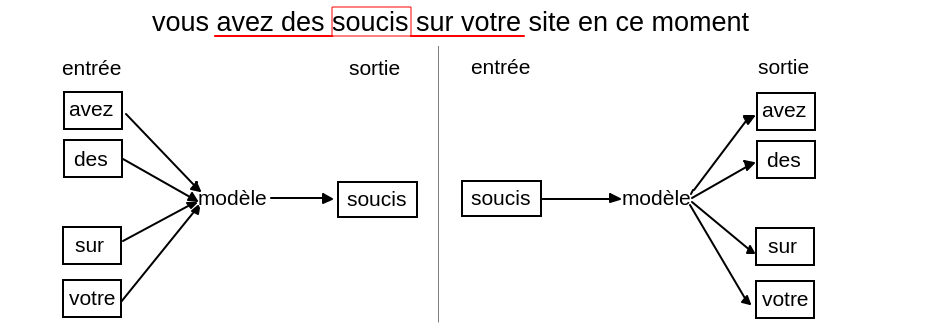
\includegraphics[width=14cm]{./Chapitre6/figures/cbow_skip.png}
    \caption{Représentation de l'apprentissage des word2vec selon deux algorithmes : le \textit{CBOW} (gauche) et le \textit{skip-gram} (droite). Ici on utilise un contexte de 5 mots, soit le mot cible entouré en rouge et deux mots de chaque coté, soulignés en rouge.
 %La partie gauche correspond à l'apprentissage avec \textit{CBOW} et la partie droite à l'apprentissage avec \textit{skip-gram}.
 }
    \label{fig:cbow_skip}
\end{figure}


Nous avons utilisé l'algorithme \textit{skip-gram} avec un contexte de 5 mots (soit le mot cible et 4 mots de contexte, 2 à gauche et 2 à droite). Le vocabulaire a été réalisé en incluant tous les mots présents dans le corpus. Tous les mots inconnus ont été remplacés lors de la transformation en une balise \textit{<UNK>} et ont donc tous la même représentation.

Afin de comparer les performances réalisées selon les différentes tailles de représentation utilisées, nous avons créé quatre ensembles de descripteurs, en faisant varier la taille des vecteurs:
\begin{itemize}
  \item \textbf{Word2vec-40} : La taille de la représentation a été fixée à 40 en raison des travaux préliminaires sur la modalité acoustique où nos représentations étaient de cet ordre de grandeur. Nous avons fait ce choix pour minimiser l'impact de la taille des descripteurs sur les performances du système,
  \item \textbf{Word2vec-100} : La taille des plongements est fixé à 100. Il s'agit d'une taille standard, beaucoup utilisée dans des tâches de NLP notamment.
  \item \textbf{Word2vec-150} : La taille des plongements est fixé à 150.
  \item \textbf{Word2vec-200} : La taille des plongements est fixé à 200. %Plus la taille des descripteurs est grande et plus on évite le sur-apprentissage généralement.
\end{itemize}

Nous avons utilisé l'architecture biLSTM-4 définie dans le chapitre~\ref{chapitre5} section~\ref{sec:5.3} pour tester la modalité linguistique représentée par des Word2vec. Les résultats sont disponibles dans le tableau~\ref{tab:res_word2vec}. Comme nous pouvons le remarquer, les scores sont supérieurs à 0.5 pour les quatre ensembles. Nous remarquons que les meilleurs scores sont atteints avec une taille de descripteurs de 100. Les performances se dégradent lorsque l'on a des tailles de descripteurs plus grandes.

Si nous comparons avec le maximum atteint par la modalité acoustique (cf section~\ref{sec:5.5.3}), soit 0.698 sur le dev et 0.513 sur le test sans post-traitement, nous voyons une amélioration de ce score maximum avec trois de nos ensembles. Avec un score CCC de 0.860 sur l'ensemble de développement et de 0.759 sur l'ensemble de test, la modalité linguistique représentée par des descripteurs Word2vec de taille 100 donne un résultat bien plus performant que tous les expérimentations effectuées sur la modalité acoustique seule.

\begin{table}[h]
  \centering
  \begin{tabular}{|l|l|l|}
  \hline
  Descripteurs   &Dev   &Test  \\
  \hline
  Word2vec-40    &0.805 &0.569 \\
  Word2vec-100   &\textbf{0.860} &\textbf{0.759} \\
  Word2vec-150   &0.592 &0.553 \\
  Word2vec-200   &0.668 &0.414 \\
  \hline
\end{tabular}
\caption{Score CCC des systèmes de reconnaissance des émotions d'une architecture neuronale bilstm à quatre couches en fonction des différents descripteurs d'entrée linguistiques.}
\label{tab:res_word2vec}
\end{table}

%\textcolor{red}{est-ce que le mauvais sscore obtenu avec word2vec-200 infirme la justification "limite le sur-apprentissage" ?}
Plusieurs justifications peuvent expliquer ce résultat. Tout d'abord, les mots sont porteurs d'informations émotionnelles qui sont moins souvent ambiguës que celles convoyées par la voix. On peut notamment mentionner les injures ou les mots contenus dans des champs lexicaux de polarité négative (par exemple ``inadmissible'', ``honteux'' ou encore ``arnaque'').

De plus, nous simplifions le travail du système de reconnaissance des émotions, puisque nous extrayons la modalité linguistique du signal audio et celle-ci est plus haut niveau. Lorsque l'on traite la modalité acoustique, les informations linguistiques sont toujours implicitement présentes et le système peut avoir des difficultés à les modéliser, notamment à cause du peu de données dont nous disposons.

De plus, les mots sont porteurs d'informations émotionnelles qui sont moins souvent ambiguës que celles convoyées par la voix. On peut notamment mentionner les injures ou les mots contenus dans des champs lexicaux de polarité négative (par exemple inadmissible, honteux ou encore arnaque).

Ces résultats nous permettent de valider l'utilisation de la modalité linguistique seule dans la détection de la satisfaction et de la frustration.

Nous avons donc chercher à tirer parti de ces deux modalités afin d'améliorer la reconnaissance de la satisfaction et de la frustration.

\section{Fusion des modalités acoustiques et linguistiques}
Comme nous l'avons défini dans le chapitre~\ref{chapitre3}, il existe plusieurs méthodes pour fusionner des modalités différentes. Chaque fusion a ses avantages et ses inconvénients et peut être plus ou moins adaptée aux descripteurs et aux modèles utilisés. Nous avons donc fait le choix de comparer les trois fusions existantes, à savoir la fusion des descripteurs, la fusion des modèles et la fusion de décision.

Ces trois fusions sont opérées sur les modalités acoustiques et linguistiques en utilisant le système biLSTM-4 précédemment introduit à la section~\ref{sec:5.3}. La figure~\ref{fig:archi_fusion} résume les quatre expérimentations dont nous rapportons les résultats dans le tableau~\ref{tab:res_fusion}.

\begin{figure}[thb]
  \centering
    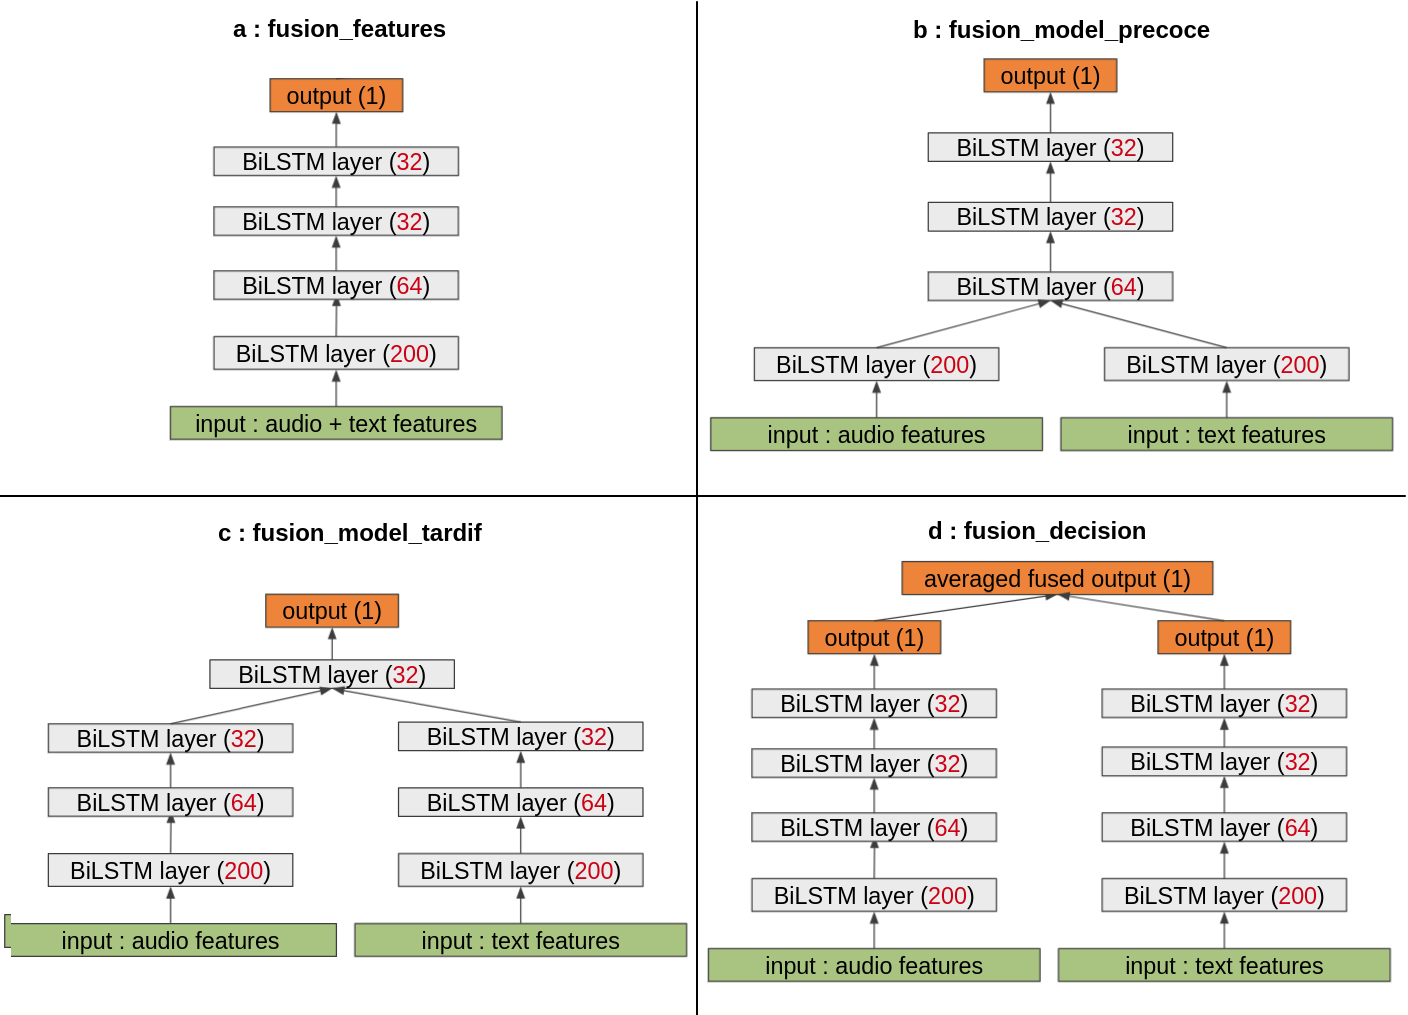
\includegraphics[width=18cm]{./Chapitre6/figures/archi_fusion.png}
    \caption{Représentation des quatre fusions utilisées pour la reconnaissance des émotions à partir des modalités acoustiques et linguistique. Les nombres entre parenthèses correspondent au nombre de neuronnes dans chaque couches.}
    \label{fig:archi_fusion}
\end{figure}


Les quatre architectures ont les caractéristiques suivantes:
\begin{itemize}
  \item \textbf{Fusion\_features} : La fusion s'effectue avant l'apprentissage en concaténant les descripteurs audio et texte. Une passe de normalisation est ensuite effectuée, pour ramener les descripteurs sur une même échelle. Il s'agit de la fusion la moins coûteuse, puisque nous n'avons qu'un seul modèle à entraîner, bien qu'il y ait plus d'entrées. Cette fusion correspond à la sous-figure a.
  \item \textbf{Fusion\_model\_precoce} : La fusion s'effectue  au niveau de la deuxième couche du réseau de neurone. Chaque modalité est d'abord traitée séparément dans la première couche, puis les deux sorties de ces deux couches sont concaténées avant d'être introduites dans la deuxième couche. La fusion précoce permet également de projeter les modalités dans des dimensions de même taille, sans pour autant que toutes les informations utiles soient déjà extraites avant d'être fusionnées. Cette fusion est modérément coûteuse, le nombre de paramètres lorsque les tailles des vecteurs d'entrée pour chaque modalité sont inférieures ou égales à 100, est du même ordre de grandeur que précédemment. Cette fusion correspond à la sous-figure b.
  \item \textbf{Fusion\_model\_tardif} : A l'inverse, la fusion va s'effectuer plus tard, au niveau de la quatrième couche du réseau. La sortie des troisièmes couches sont concaténées avant d'être données à la quatrième couche. Ce fusion tardive va prendre en compte des descripteurs très modifiés, desquels les informations importantes sont normalement déjà extraites. Cette fusion correspond à la sous-figure c.
  \item \textbf{Fusion\_decision} : Cette fusion s'effectue sur les sorties des deux modèles. On entraîne séparément deux modèles pour les deux modalités, puis on met en concours les deux vecteurs de sorties des deux modèles en utilisant une moyenne pondérée ou non. Cette fusion est la plus coûteuse puisque nous apprenons deux modèles distincts et que nous appliquons un post-traitement sur les sorties de ces modèles. Cette fusion correspond à la sous-figure d.
\end{itemize}

\begin{table}[h]
  \centering
  \begin{tabular}{|l|l|l|}
  \hline
  Descripteurs   &Dev   &Test  \\
  \hline
  \multicolumn{3}{|l|}{fusion features} \\
  \hline
  MFCC $\oplus$ word2vec-40        &.895  & .833 \\
  MFCC $\oplus$ word2vec-100        &.836  & .788 \\
  \hline
  \multicolumn{3}{|l|}{fusion modèle précoce} \\
  \hline
  MFCC-lib $\oplus$ word2vec-40       & .904 & .807 \\
  MFCC-lib $\oplus$ word2vec-100       & .829 & .797 \\
  \hline
  \multicolumn{3}{|l|}{fusion modèle tardive}   \\
  \hline
  MFCC-lib $\oplus$ word2vec-40    & .917  & .815  \\
  MFCC-lib $\oplus$ word2vec-100    & .881  & .717  \\
  \hline
  \multicolumn{3}{|l|}{fusion décision} \\
  \hline
  .66 Word2vec-40 + .34 MFCC-lib     &.897  &.840  \\
  .72 Word2vec-100 + .28 MFCC-lib    &.844 & .789 \\
  \hline
\end{tabular}
\caption{Comparaison des score CCC des systèmes de reconnaissance des émotions du biLSTM-4 en utilisant différent protocole de fusion et différents descripteurs pour la modalité linguistique.}
\label{tab:res_fusion}
\end{table}

Les résultats de ces différentes fusions sont disponibles dans le tableau~\ref{tab:res_fusion}. Nous observons que les scores de fusion, quelqu'ils soient, permettent d'égaler ou d'améliorer les résultats unimodaux. Nous remarquons que dans tous les types de fusion, c'est l'utilisation des word2vec-40 qui donne de meilleurs résultats. Cela peut être dû à la similarité entre les dimensions acoustiques et linguistiques : les MFCC-lib sont constitués de 48 descripteurs.
Nous pouvons également noter que le meilleur score atteint sur l'ensemble de dev ($0.917$) est attribué à la fusion tardive de modèle. Cependant, nous voyons que ce n'est pas la fusion de modèle qui donne le meilleur résultat sur l'ensemble de test. Le meilleur score ($0.840$) est atteint avec la fusion tardive. De plus l'écart entre le score de dev et de test est moins important pour la fusion tardive. Nous avons donc décidé de conserver la fusion tardive comme fusion de référence dans la suite de nos expérimentations.

Comme nous l'avons déjà présenté dans le chapitre~\ref{chapitre3}, les word2vec sont statiques : un mot a toujours la même représentation vectorielle, quel que soit le vrai sens du mot et le contexte de son apparition. Cela peut être problématique pour les mots polysémiques, par exemple fréquents en français~\cite{Pustejovsky1996}. C'est pour cette raison que nous avons souhaité mettre en place des représentations permettant de prendre en compte le contexte, que ce soit sur l'acoustique ou sur le linguistique.

\section{Descripteurs pré-entraînés}

L'apprentissage par transfert, \textit{transfert-learning} est largement utilisé dans l'analyse des sentiments, où de grandes bases de données non spécifiques sont utilisées pour former des caractéristiques génériques qui sont introduits dans le processus d’apprentissage.
Ce procédé permet de donner aux systèmes de meilleures capacités de généralisation compte tenu des données d'apprentissage fortement limitées~\cite{Dong2018}.

Une autre méthode permettant d'exploiter des modèles qui ont déjà vu une très grande quantité de données est d'utiliser des représentations auto-apprises. L'apprentissage auto-supervisé des représentations de la parole ou du langage a été proposé ces dernières années, par exemple avec le système BERT~\cite{Devlin2019}, utilisé pour la représentation textuelle que nous avons présenté au chapitre~\ref{chapitre2}.

De telles représentations, calculées par des modèles neuronaux entraînés sur d'énormes quantités de données non étiquetées, ont montré leur efficacité, par exemple pour la vision par ordinateur~\cite{Nanni2017} et des tâches de traitement du langage naturel (NLP) telles que de la
classification, de la similarité de texte, ou du classement par pertinence~\cite{Liu2019,Young2018,Yang2019}. Ils ont également prouvés leur efficacité dans les domaines de l'ASR~\cite{Kahn2020,Liu2020} et de la traduction~\cite{Nguyen2020}.

Néanmoins, ces représentations n'avaient jamais été utilisé pour de la reconnaissance d'émotions continues à notre connaissance. Nous avons donc proposé de tester cette approche pour réaliser notre tâche de reconnaissance des émotions. Il n'est, en effet, pas évident qu'elle soit pertinente pour la SER. Par exemple, au niveau acoustique, l'ASR a tendance à se concentrer sur des durées d'environ 30 ms, tandis que les émotions sont généralement prises en charge sur environ 1 seconde de parole.

Nous pensons que l'utilisation de ces représentations peut limiter l'impact du manque de données lorsque seules de petites bases de données sont disponibles pour former un réseau de neurones pour une tâche spécifique.

\subsection{Représentation linguistique}
Pour modéliser la partie linguistique, nous sommes partis sur des systèmes dérivés de BERT. Comme nous l'avons défini dans le chapitre~\ref{chapitre2}, BERT permet de donner une représentation contextuelle du texte. Il est cependant appris en majorité avec des occurrences anglaises. Comme nous voulons modéliser du français, nous nous sommes tournés vers CamemBERT~\cite{Martin2020} et FlauBERT~\cite{Le2020} que nous avons présenté également au chapitre~\ref{chapitre2}.

Chronologiquement, nous avons découvert CamemBERT en premier, et une fois que nous avions expérimenté avec ce modèle, nous avons comparé les résultats obtenus avec le modèle FlauBERT.

Pour l'extraction des descripteurs, nous avons utilisé le toolkit Fairseq~\cite{Ott2019}. Nous utilisons le modèle pré-entraîné, appelé \textit{camemBERT-base}, entraîné sur la partie française du corpus OSCAR~\cite{Ortizsuarez2019} constitué d'un ensemble de corpus monolingues extraits du \textit{Common Crawl snapshot} et totalisant 138Go de texte brut et 32,7 milliards de tokens après la tokenisation en sous-mots~\cite{Wu2016}. Les sous-mots sont des ensembles de caractères qui ne sont pas des mots à proprement parlé et qui sont déduit par le système de tokenisation, ici SentencePiece~\cite{Kudo2018}.

Les caractéristiques ont été extraites sur Allosat à l'aide de ce modèle pré-entraîné, et nous avons résumé les résultats au niveau du segment émotionnel (250~ms) en faisant la moyenne des représentations continues des sous-mots apparaissant dans le segment courant. Au total, nous utilisons un vecteur de caractéristiques à 768 dimensions.

Nous voulions également utiliser la variance de ces représentations, dans une volonté de comparer nos représentations aux précédentes qui utilisaient à la fois la moyenne et la variance des descripteurs. Cependant doubler le nombre de caractéristiques faisait exploser la complexité du réseau et donc le temps d'apprentissage.

Les résultats sont présentés dans le tableau~\ref{tab:res_camembert}. Comme nous pouvons l'observer, les modèles sont très performants pour la reconnaissance des émotions continues. Les descripteurs issus de CamemBERT donnent de meilleurs résultats que ceux issus de FlauBERT même s'ils restent du même ordre de grandeur. Si on se compare aux meilleurs résultats des word2vec, à savoir respectivement $0.860$ et $0.759$ sur le dev et le test, on obtient une amélioration du score CCC de 0$.036$ sur le dev et de $0.040$ sur le test.

\begin{table}[h]
  \centering
  \begin{tabular}{|l|l|l|}
  \hline
  Descripteurs   &Dev   &Test  \\
  \hline
  CamemBERT      &\textbf{0.896} &\textbf{0.799} \\
  FlauBERT       &0.874 &0.733 \\
  \hline
\end{tabular}
\caption{Scores CCC des systèmes de reconnaissance des émotions du biLSTM-4 en prenant en entrée des descripteurs linguistiques pré-entrainés.}
\label{tab:res_camembert}
\end{table}


\subsection{Représentation acoustique}
Dans le domaine du SER, trouver le meilleur ensemble de caractéristiques acoustiques est toujours un sous-domaine de recherche actif~\cite{Jing2018}.

Comme nous l'avons déjà dit (cf section~\ref{sec:3.3.1}), la plupart des ensembles de caractéristiques \textit{experts}~\cite{Eyben2016,Schuller2013} visent à décrire la prosodie dans le signal, avec des descripteurs de bas niveau (LLD) capturant l'intensité, l'intonation, le rythme ou la qualité de la voix.
Une autre approche consiste à extraire des caractéristiques spectrales : les coefficients cepstraux à fréquence mel (MFCC) sont clairement les plus utilisés car ils sont robustes aux signaux bruités même s'ils n'ont pas été conçus pour la prosodie ou l'émotion.

Récemment, wav2vec~\cite{Schneider2019} et Audio AlBERT~\cite{Chi2020} ont été introduits dans les domaines de la reconnaissance automatique de la parole et dans l'identification du locuteur comme l'une des premières approches pré-entraînées pour extraire des caractéristiques contextuelles des signaux bruts.
Comme nous l'avons expliqué au chapitre~\ref{chapitre2}, wav2vec~\cite{Schneider2019} est un modèle pré-entraîné par auto-supervision : il apprend à prédire les futurs échantillons à partir de l'une analyse de le fenêtre courante.

Dans nos expérimentations, nous utilisons deux modèles pré-entraînés. Le premier, appelé \textit{wav2vec-EN}, fourni par Schneider et al.,  a été entraîné sur le corpus Librispeech~\cite{librispeech} qui est composé de 960 heures de livre audio en anglais.
Nous formons également notre propre modèle, appelé \textit{wav2vec-FR}, dérivé du premier modèle et fine-tuné sur les conversations non étiquetées de centres d'appels français correspondant à plus de 500 heures de données privées.

Comme ce modèle est appris avec des audios échantillonnés à 16kHz, nous avons sur-échantillonné nos données pour qu'elles correspondent aux modèles. Nous avons utilisé la fonction de rééchantillonnage FFMpeg~\cite{Tomar2006} avec la fonction d'interpolation \textit{sinc}.

Au final, chaque segment émotionnel est représenté par un vecteur de taille 512 qui se compose des valeurs moyennes des plongements obtenus toutes les 10~ms sur le segment émotionnel, \textit{i.e.} soit une moyenne de 25 valeurs pour AlloSat. Comme pour la représentation linguistique, nous avons uniquement conservé la moyenne et non l'écart type pour de pas avoir des vecteurs d'entrée trop important qui aurait fait exploser la complexité et donc le temps d'apprentissage et les ressources nécessaires pour le mener à bien.

\begin{table}[h]
  \centering
  \begin{tabular}{|l|l|l|}
  \hline
  Descripteurs   &Dev   &Test  \\
  \hline
  wav2vec-EN      &0.851 &\textbf{0.730} \\
  wav2vec-FR      &\textbf{0.865} &0.635 \\
  \hline
\end{tabular}
\caption{Score CCC des systèmes de reconnaissance des émotions du biLSTM-4 en prenant en entrée des descripteurs acoustiques pré-entrainés.}
\label{tab:res_wav2vec}
\end{table}


Les résultats sont présentés dans le tableau~\ref{tab:res_wav2vec}. Comme nous pouvons l'observer, les modèles sont également très performants pour la reconnaissance des émotions continues. Les descripteurs issus de wav2vec-EN donne de meilleurs résultats que ceux issus de wav2vec-FR même s'il reste dans la même ordre de grandeur. Cela peut être expliqué par le fine-tuning effectué sur à peine 500 heures de données, ce qui a pu suffisamment dérégler le modèle sans pour autant lui faire intégrer des renseignements pertinents. Si on se compare aux meilleurs résultats des MFCCs, à savoir respectivement $0.698$ et $0.513$ sur le dev et le test, on peut affirmer que la représentation wav2vec-EN permet au système de mieux reconnaître les états émotionnels, puisqu'on améliore les scores respectivement de $0.153$ et $0.217$ sur le dev et le test.

\subsection{Reproduction sur SEWA}
Afin d'étendre l'utilisation des descripteurs pré-entraînés, nous avons voulu tester les performances d'un système biLSTM-4 apprenant avec ce type de descripteurs pour le corpus SEWA. Le corpus étant en allemand et en hongrois, nous avons uniquement considéré le modèle wav2vec-EN.

\begin{table}[h]
  \centering
  \begin{tabular}{|l|l|l|l|}
  \hline
  Descripteurs   &Activation   &Valence  &Liking  \\
  \hline
  wav2vec-EN      &0.251      &0.215      &0.254 \\
  \hline
\end{tabular}
\caption{Scores CCC des systèmes de reconnaissance des émotions du biLSTM-4 en prenant en entrée des descripteurs acoustiques pré-entrainés sur l'ensemble de dev du corpus SEWA.}
\label{tab:sewa_wav2vec}
\end{table}


Les résultats sont présentés dans le tableau~\ref{tab:sewa_wav2vec}. Les scores obtenus sur les dimensions de l'activation et de la valence sont moins élevés que lorsque l'on utilise les ensembles de descripteurs MFCCs ou eGeMAPS. Cependant on peut constater une amélioration sur l'axe du liking, mais qui n'atteint pas un score suffisant pour être considéré comme une réussite.

Dans le cas du corpus SEWA, l'utilisation de descripteurs pré-entraînés ne semble pas permettre d'améliorer les performances du système. Notre hypothèse réside dans la différence de quantité de données entre les deux corpus : le set de train d'AlloSat est composé de 25 heures d'enregistrement audio alors que celui de SEWA a moins de 2 heures de conversations. %Malgré l'utilisation des descripteurs pré-entraînés, le réseau n'est pas en mesure d'obtenir de bons résultats, probablement en raison de la faible quantité de données.
Nous pensons également que la conception du corpus SEWA peut avoir un impact sur la performance de ces descripteurs. Le fait que SEWA soit composé de conversations dyadiques où deux locuteurs sont présents dans le même document peut complexifier le processus d'extraction de descripteurs, alors qu'AlloSat ne contient que la voix du client.

Nous avons vu précédemment que la fusion des deux modalités, en considérant les descripteurs MFCC et word2vec, permet d'améliorer les performances du système. Nous expérimentons donc la fusion des descripteurs pré-appris.

\section{Fusion des modalités acoustiques et linguistiques pré-entraînés}
Différents protocoles de fusion ont été explorés : fusion features (concaténation des vecteurs wav2vec et camemBERT), fusion au niveau du modèle (au niveau de la première et de la dernière couche) et fusion de décision. Les fusions features et au niveau du modèle requièrent beaucoup plus de temps d'apprentissage, puisque nous doublons le nombre d'entrées du réseau (768+512). De plus, les résultats que nous avons obtenus sur ces features sont peu intéressants puisqu'au niveau des scores d'unimodalité. Nous ne les présentons pas dans ce document.

Comme jusqu'à présent la modalité linguistique donne de meilleurs résultats que la modalité acoustique et que la dimension des descripteurs camemBERT est grande, nous avons voulu quantifier l'apport de ces descripteurs en les comparant aux descripteurs word2vec. Ainsi en fonction de l'ordre de grandeur de cet apport, nous pourrons statuer sur la pertinence ou non de l'utilisation de plus de ressources.

\begin{table}[h]
  \centering
  \begin{tabular}{|l|l|l|l|}
  \hline
  Descripteurs &nombre features   &Dev   &Test  \\
  \hline
  %\multicolumn{4}{|l|}{fusion décision} \\
  %\hline
  .66 word2vec-40 + .34 MFCC-lib     &47 + 40 &0.897  &0.840  \\
  .63 wav2vec-EN + .37 word2vec      &512 + 40 &0.878 &0.750 \\
  .28 wav2vec-EN + .72 CamemBERT        &512 + 768 &\textbf{0.932} &\textbf{0.920} \\
  %.31 wav2vec-EN + .69 camemBERT     &512 + 768 &\textbf{0.907}   &\textbf{0.825} \\
  \hline
\end{tabular}
\caption{Comparaison des score CCC des systèmes de reconnaissance des émotions du biLSTM-4 en utilisant la fusion de décision avec des descripteurs pré-entrainés. Nous rappelons les scores obtenus précédemment avec la fusion des descripteurs baseline.}
\label{tab:res_fusion_pretrain}
\end{table}


Comme pour les résultats précédents sur la fusion des descripteurs de la baseline (MFCC + word2vec), la fusion de décision permet d'améliorer les résultats même si l'amélioration est moins forte que précédemment. Comme nous le rapportons dans le tableau~\ref{tab:res_fusion_pretrain}, nous atteignons des scores de $0.932$ sur le dev et $0.920$ sur le test, ce qui correspond à une augmentation significative des scores. On remarque également que la fusion des ensembles wav2vec-EN et word2vec donne de moins bons résultats, et que c'est la modalité acoustique qui prime dans cette fusion. On peut supposer que la trop grosse différence dans le type de descripteur ne va pas permettre une bonne fusion.

Nous atteignons donc des scores très performants pour la reconnaissance des émotions continues sur le corpus AlloSat, permettant à l'entreprise de penser à la commercialisation de cet indicateur.

\section{Conclusion}
Dans ce chapitre, nous avons décrit les différents choix que nous avons considéré pour améliorer nos performances en terme de reconnaissance continue des émotions. Après une discussion autour de la confiance dans les scores CCC, nous avons mis en place une représentation linguistique des conversations que nous avons fusionné avec la représentation acoustique. De plus, nous avons mis en place des nouveaux modèles entraînés avec des descripteurs pré-entraînés.

Nous pouvons conclure que le meilleur système de reconnaissance des émotions continues utilise un réseau de neurones récurrents, une utilisation des deux modalités en les fusionnant et des entrées issues de descripteurs pré-entraînés.

Ces scores a l'état de l'art sont très corrects, mais une question reste en suspens : pourquoi la modalité linguistique permet une telle amélioration de la reconnaissance continue des émotions ? Nous allons tenter de répondre à cette question dans le prochain chapitre.


% \clearemptydoublepage
% \chapter{Analyse des annotations, explicabilité des modèles autour de la frustrations}
\label{chapitre7}

\section{Motivations}
Lors de cette thèse, nous avons établi des systèmes de reconnaissance continue de l'émotion qui permettent de détecter la satisfaction et la frustration avec un degré d'erreur \textcolor{blue}{acceptable}.
Dans ce dernier chapitre, nous avons voulu questionner la stratégie qui consiste à fusionner les annotations individuelles de chaque annotateurs.
Ainsi nous souhaitons proposer une alternative à la conception la plus établie en matière d'annotation en émotion.
Dans un second temps, la modalité linguistique étant celle qui induit les meilleures performants, il nous semblait important d'essayer de comprendre la prévalence de cette modalité.

Dans la littérature, on a pour habitude d'utiliser de nombreux annotateurs et de fusionner les annotations pour atténuer le caractère subjectif d'une annotation. En effet, il est difficile de nier que la reconnaissance d'une émotion et de son intensité peut varier en fonction de la personne qui la perçoit. Il est donc possible d'avoir autant de versions différentes des annotations que d'annotateurs. Dans ce cas, ne peut-on pas considérer que chaque annotateur est dans le juste ? Nous analysons ce positionnement dans la prochaine section.

Comme nous l'avons établi dans le précédent chapitre, nous pouvons observer que la modalité linguistique permet d'atteindre les meilleurs scores de reconnaissance continue des émotions de satisfaction et de frustration contenues dans AlloSat. Nous aurions pensé dans un premier temps que la modalité acoustique donnerait de meilleurs résultats. En effet, la modalité acoustique, telle que nous la traitons, contient déjà les informations linguistiques. Elles ne sont pas extraites et pré-traitées mais nous pensions que le système de reconnaissance serait capable d'en retirer les informations pertinentes.

Nous avons donc cherché les marqueurs de l'émotion dans les transcriptions des conversations téléphoniques. Nous avons d'abord conduit des analyses statistiques sur le corpus, puis nous avons travaillé avec un linguiste du LIUM, Pr. Daniel Luzzati, afin de retrouver les clés permettant à l'humain de reconnaître les états émotionnels de satisfaction et de frustration.

\section{Analyse de l'impact de chaque annotateur}

\subsection{Annotation moyenne ou 3 annotations ?}
Comme nous l'avons vu dans le chapitre~\ref{chapitre4}, nous avons choisi de faire annoter le corpus par trois annotateurs. Ce choix a été motivé par l'aspect subjectif non négligeable de toutes les tâches mettant en œuvre des émotions. Nos données contiennent donc des conversations qui ont été annotées trois fois, comme par exemple la conversation illustrée par la Figure~\ref{fig:annotTroisGold}. On peut observer une tendance globale commune entre les annotations avec des différences en intensité et en délais avant de noter un changement d'émotions. Deux positionnements peuvent être pris à partir de ces annotations.

\begin{figure}[h]
  \centering
  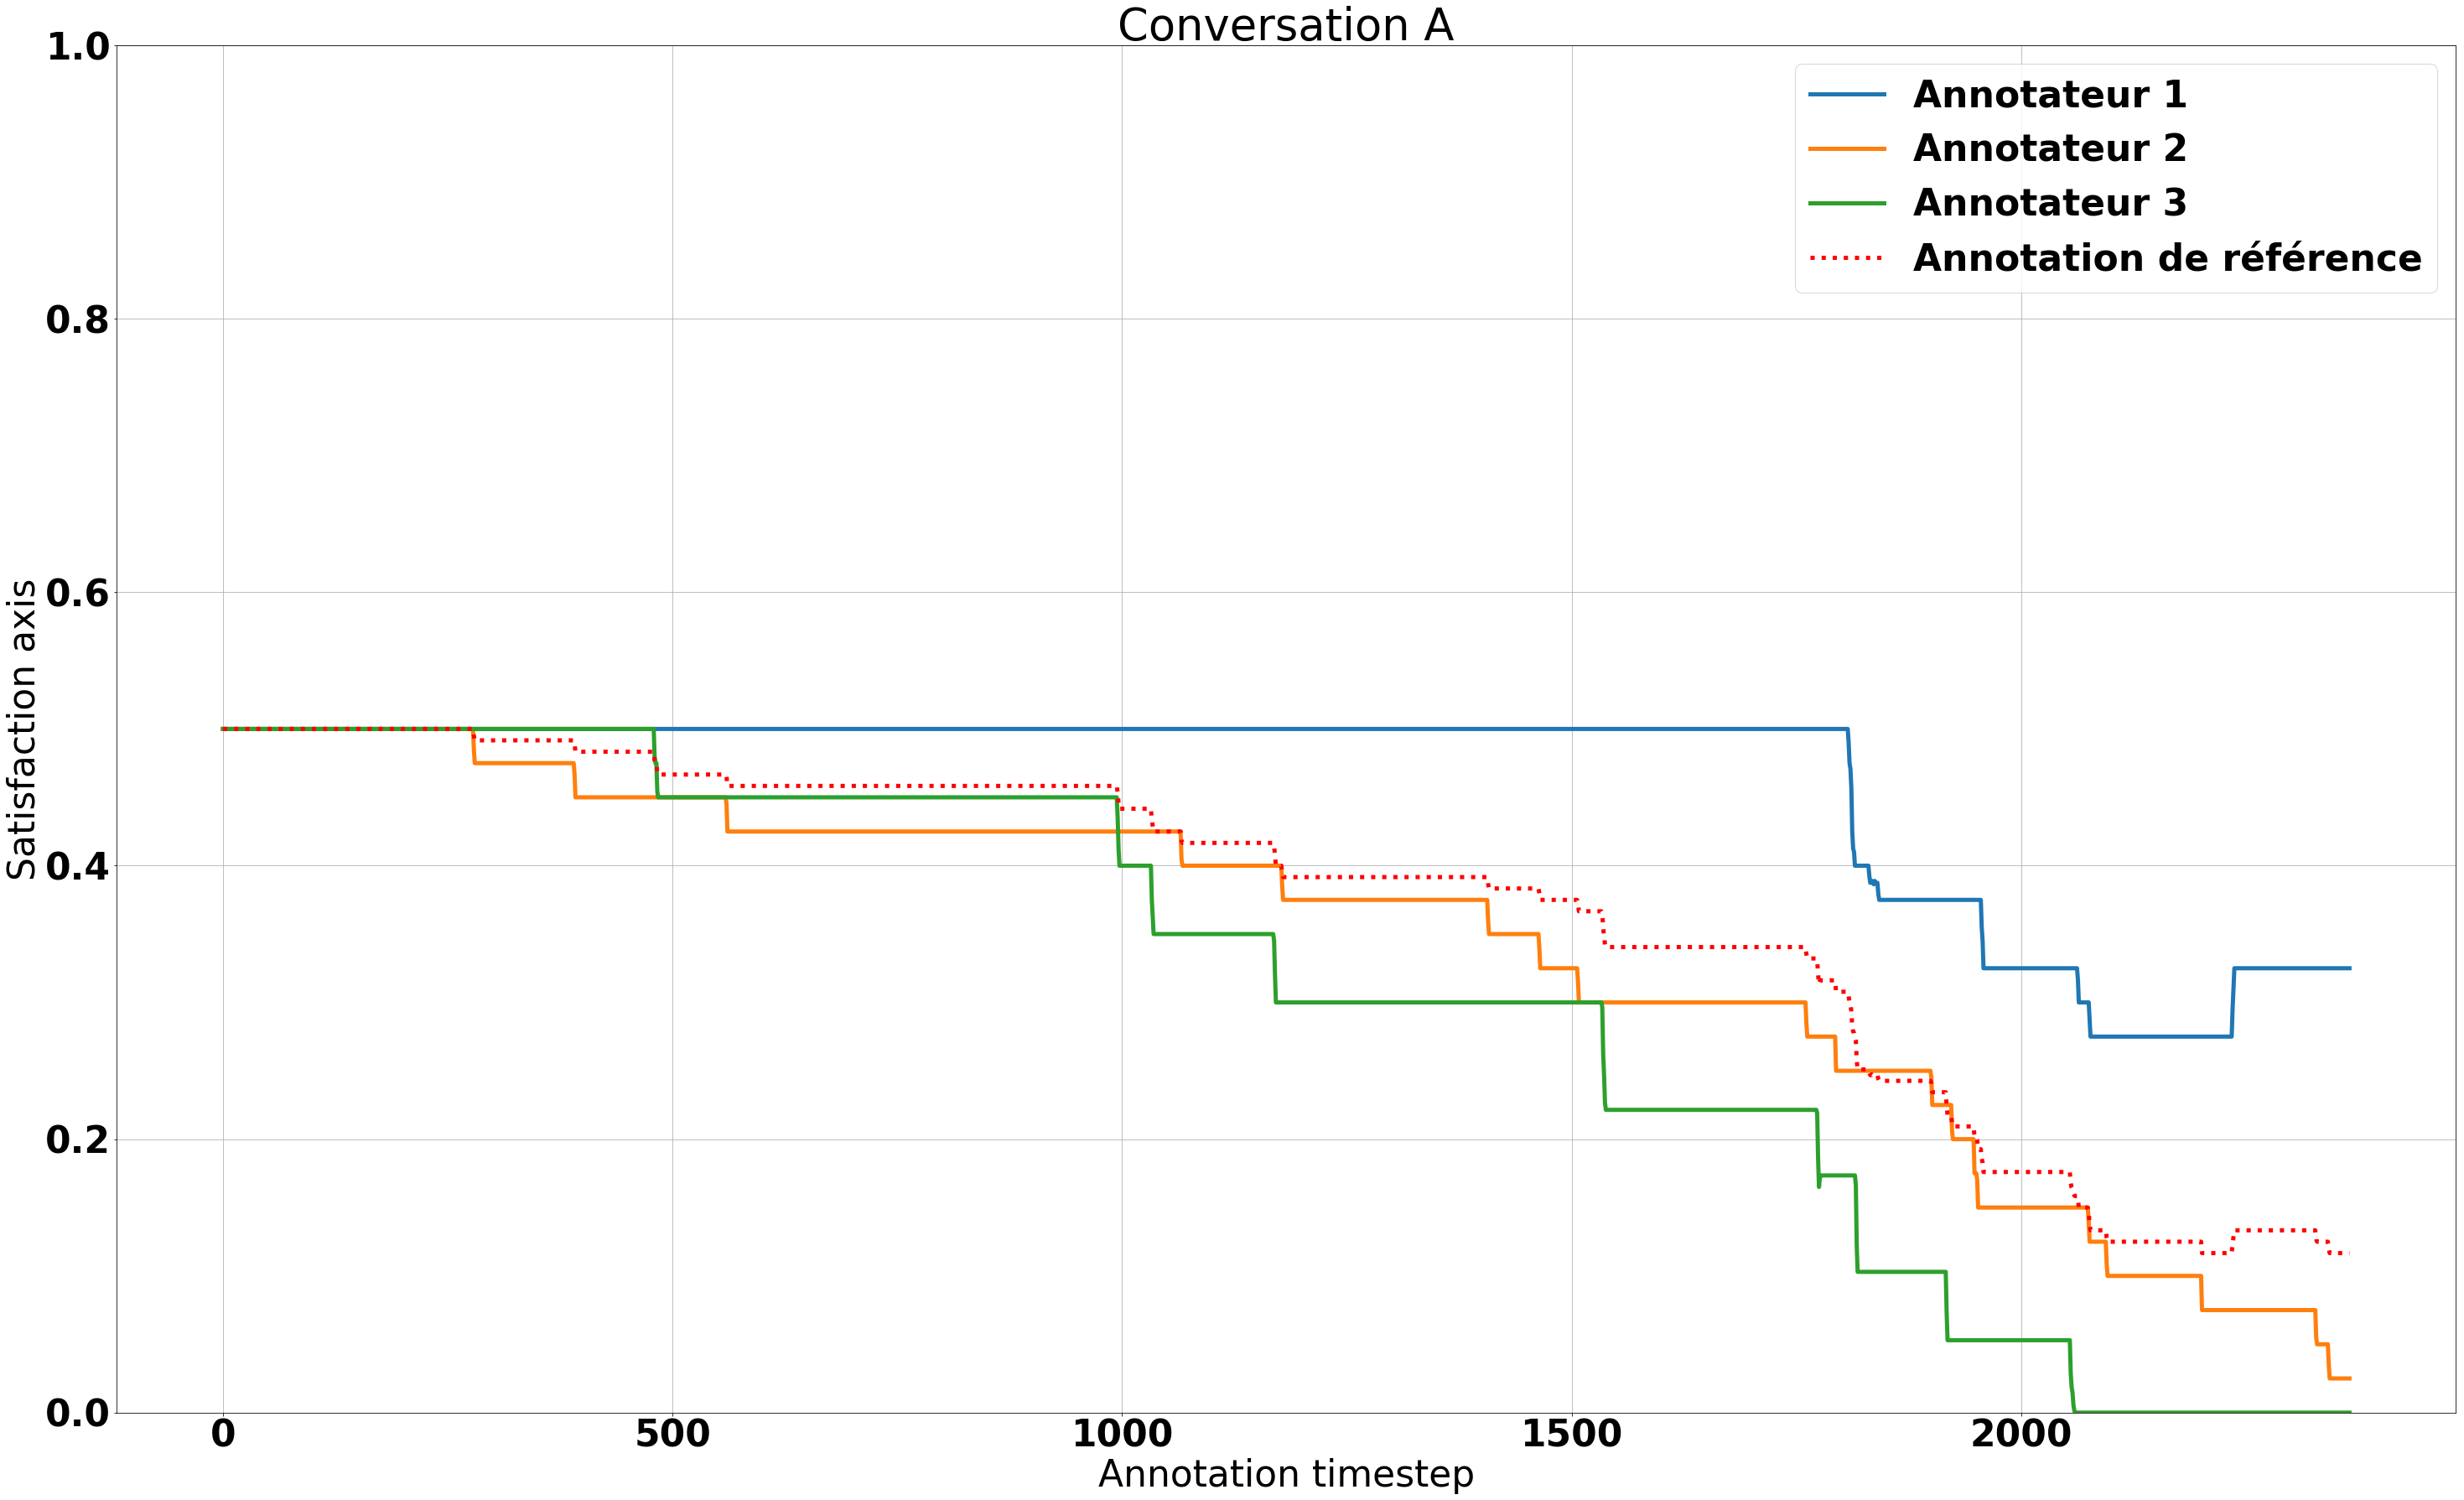
\includegraphics[width=15cm]{./Chapitre7/figures/annotTroisGold.png}
  \caption{Exemple d'annotation d'une conversation selon l'axe de satisfaction deja présenté chapitre 4. L'annotation de référence correspond à la courbe en pointillée}
  \label{fig:annotTroisGold}
\end{figure}


\begin{enumerate}
  \item Nous pouvons considérer les annotations de chaque annotateur indépendamment. En effet, nous pouvons partir du principe que la perception de l'émotion par chaque individu est légitime et peut être considérée comme une référence pour le système de détection.
  Ce positionnement va donc considérer que l'individu a plus de valeur que le groupe entier. Nous pouvons donc spécifier nos systèmes de reconnaissance pour reproduire le comportement d'un humain particulier.
  \item Nous pouvons également considérer la moyenne des annotations. En effet, faire la moyenne des annotations revient à généraliser ces dernières pour qu'elles soient plus en adéquation avec un ensemble d'individus et atténuer les perceptions qui s'écartent d'une normalité statistique. Ainsi, nous allons considérer que l'annotation de référence pour nos systèmes automatiques est la moyenne de l'avis de différentes personnes. Bien que ce procédé soit plus pertinent lorsque nous avons un nombre élevé d'annotateurs, il reste cohérent pour trois annotateurs et permet de généraliser nos systèmes de reconnaissance pour reproduire non pas le comportement d'un humain particulier mais d'un groupe d'humain.
\end{enumerate}

Au cours de la thèse, nous avons décidé, en adéquation avec les besoins industriels, de nous concentrer sur le deuxième positionnement, comme nous l'avons énoncé dans le chapitre~\ref{chapitre4}. Ce positionnement est également celui de nombreux travaux dans le domaine, notamment les travaux effectués sur les corpus RECOLA~\cite{Ringeval2013} et SEWA~\cite{SEWA}.

Cependant pour aller plus loin dans l'analyse du phénomène émotionnel, nous avons voulu explorer la possibilité d'utiliser les annotations de chacun afin de construire des systèmes de reconnaissance.

\subsection{Un modèle de reconnaissance par annotateur}
Si nous considérons que chaque annotateur donne une version légitime de l'émotion, nous pouvons choisir de construire trois modèles de reconnaissance en prenant les annotations des trois annotateurs. Pour ce faire, nous modifions la référence : au lieu d'entraîner un seul modèle sur la valeur moyenne des trois annotateurs, nous entraînons trois modèles différents par annotateur, dans lesquels les références correspondent aux valeurs uniques de cet annotateur.
Les prédictions de ces modèles sont évaluées en fonction des annotations individuelles (tableau~\ref{tab:ind_by_annotator}) ou de nos anciennes références définies comme la moyenne des trois annotations individuelles (tableau~\ref{tab:moy_by_annotator}).

Les colonnes AVG donnent les performances moyennes sur les trois modèles individuels. Les colonnes CV donnent le coefficient de variation (écart-type sur la moyenne) sur les trois modèles individuels. Diff1 est la différence relative entre linguistique et acoustique pris indépendamment et donne une idée du gain par annotateur.

\subsubsection{Annotations individuelles : }

\begin{table}[h]
    \centering
    \begin{tabular}{| l |cc| cc | cc | cc | cc |}\hline
     \textbf{Annotateurs} & \multicolumn{2}{c|}{$a_1$} & \multicolumn{2}{c|}{$a_2$}  &\multicolumn{2}{c|}{$a_3$} &\multicolumn{2}{c|}{AVG} & \multicolumn{2}{c|}{CV}\\
      & \textbf{Dev} &\textbf{Test} &\textbf{Dev}  &\textbf{Test} & \textbf{Dev} &\textbf{Test} & \textbf{Dev} &\textbf{Test} & \textbf{Dev} &\textbf{Test}\\ \hline

     Wav2Vec    & .834 & .734 & .731 & .785 & .841 & .597 & .802 & .705 & .077 & .138\\
     CamemBERT  & .898 & .877 & .833 & .834 & .900 & .804 & .877 & .838 & .043 & .044\\
     Diff1 (\%)           & 7.7 & 19.5 & 14.0 & 6.2 & 7.0 & 34.7 & - & - & - & -\\
     \hline
     Features              & .884 & .870 & .815 & .753 & .883 & \textbf{.834} & .861 & .819 & .046 & .073 \\
     \hline
     Modèle précoce    & .883 & .870 & \textbf{.855} & \textbf{.865} & .888 & .826 & .875 & \textbf{.854} & .020 & .028\\
     Modèle tardive     & .911 & .875 & .814 & .837 & \textbf{.921} & .799 & .882 & .837 & .067 & .045\\
     \hline
     Décision           & \textbf{.913} & \textbf{.882} & .840 & .849 & .916 & .793 & \textbf{.890} & .841 & .048 & .053 \\
     \hline

    \end{tabular}
    \caption{Résultats des systèmes de fusions pour chaque annotateur. Les modèles sont entraînés et évalués sur des annotations individuelles. AVG : moyenne sur les trois annotateurs. CV : coefficient de variation sur les trois annotateurs. Diff1 correspond à la différence absolue entre CamemBERT et Wav2Vec. La meilleure fusion est choisie sur le Dev.}
    \label{tab:ind_by_annotator}
\end{table}


Dans le tableau ~\ref{tab:ind_by_annotator}, nous pouvons remarquer que le coefficient de variation (CV), sans utiliser de fusions, est plus élevé avec les descripteurs acoustiques qu'avec les descripteurs linguistiques en particulier sur le Test. Plus précisément, concernant l'annotateur $a_3$, les performances de la modalité acoustique chutent sur le Test pour atteindre un score CCC de 0.597.
Ces résultats suggèrent que la prédiction de la satisfaction à partir des descripteurs acoustiques est plus sensible à la subjectivité de la tâche d'annotation qu'à partir des descripteurs linguistiques.

Notre hypothèse est que la variabilité dans l'espace acoustique est très diversifiée, et qu'une même réalisation acoustique peut être perçue avec des niveaux de satisfaction différents par le même annotateur, ce qui produit de moins bonnes performances sur la modalité acoustique.

En ce qui concerne la fusion des modalités, elle améliore les performances dans la plupart des configurations et les meilleures performances en moyenne sont atteintes avec la fusion modèle précoce avec un score de CCC de 0.854 sur l'ensemble de Test. L'amélioration sur le Test est la plus élevée avec l'annotateur $a_2$ ($+3.7$\% avec la fusion modèle précoce).
Cela peut s'expliquer par la très faible différence entre les performances obtenues sur des modalités acoustiques et linguistiques pour cet annotateur ($+6.2$\%), indiquant peut-être que les deux modalités portent des informations différentes pour cet annotateur spécifique.

A partir de ces résultats, nous émettons l'hypothèse qu'au niveau des annotateurs, les modalités acoustiques et linguistiques véhiculent des informations émotionnelles complémentaires. Cependant, si la partie linguistique est bien partagée entre les annotateurs, la perception de la partie acoustique semble assez individuelle.
Bien sûr, des expériences supplémentaires avec des annotations croisées sont nécessaires pour confirmer cette hypothèse.

\subsubsection{Annotations moyennes : }

\begin{table}[h]
    \centering
    \begin{tabular}{|l |cc| cc | cc | cc | cc|}\hline
     \textbf{Annotateurs} & \multicolumn{2}{c|}{$a_1$} & \multicolumn{2}{c|}{$a_2$}  &\multicolumn{2}{c|}{$a_3$} &\multicolumn{2}{c|}{AVG} & \multicolumn{2}{c|}{CV}\\
      & \textbf{Dev} &\textbf{Test} &\textbf{Dev}  &\textbf{Test} & \textbf{Dev} &\textbf{Test} & \textbf{Dev} &\textbf{Test}  & \textbf{Dev} &\textbf{Test}\\ \hline

     Wav2Vec    & .862 & .736 & .774 & .731 & .779 & .710 & .805 & .726 & .061 & .019\\
     CamemBERT  & .916 & .878 & .755 & .793 & .851 & .833 & .841 & .835 & .096 & .051\\
     Diff1 (\%)           & 6.3 & 19.3 & -2.5 & 8.5 & 9.2 & 17.3 & - & - & - & -\\
     \hline
     Features           & .896 & .845 & .741 & .688 & .868 & .861 & .835 & .798 & .099 & .120 \\
     \hline
     Modèle précoce     & .911 & .833 & \textbf{.809} & \textbf{.824} & \textbf{.879} & .856 & .866 & .838 & .060 & .020\\
     Modèle tardive      & .914 & \textbf{.899} & .763 & .784 & .844 & .841 & .840 & .841 & .090 & .068\\
     \hline
     Décision           & \textbf{.938} & .882 & .795 & .778 & .868 & \textbf{.874} & \textbf{.867} & \textbf{.845} & .082 & .069 \\
     \hline

    \end{tabular}
    \caption{Résultats des systèmes de fusions pour chaque annotateur. Les modèles sont entraînés sur des annotations individuelles et évalués sur les annotations moyennés de référence. AVG : moyenne sur les trois annotateurs. CV : coefficient de variation sur les trois annotateurs. Diff1 correspond à la différence absolue entre CamemBERT et Wav2Vec. La meilleure fusion est choisie sur le Dev.}
    \label{tab:by_annotator}
\end{table*}


En ce qui concerne les modèles individuels évalués avec des annotations moyennes (tableau ~\ref{tab:moy_by_annotator}), nous remarquons que l'annotateur $a_2$ a les performances les plus faibles lorsqu'il utilise uniquement des descripteurs linguistiques.
Le modèle construit sur cet annotateur atteint les performances les plus basses en utilisant n'importe quel type de fusion sur les ensembles de Développement et de Test.
Cette observation confirme ainsi l'importance des performances linguistiques qui ont un poids important dans l'évaluation générale de la satisfaction et la frustration quand on fusionne les modalités.
Ce résultat peut s'expliquer par le fait que parmi les trois annotateurs, nous avons montré que $a_2$ avait l'accord intra-annotateur le plus faible dans le chapitre~\ref{chapitre4}.

Nous pouvons également confirmer le fait que la fusion permet d'améliorer les performances par annotateur dans tous les cas.
Étonnamment, sur le Test, ces modèles fusionnés (CCC=0.884) surpassent même les modèles appris directement sur la référence traditionnelle (meilleur CCC=0.881). Néanmoins comme nous l'avons vu dans le chapitre~\ref{chapitre6}, une différence de 0.003 entre deux scores de CCC n'est pas vraiment significative.
La fusion modèle précoce a l'avantage d'avoir des performances moyennes plus élevées que CamemBERT et d'être le modèle le moins affecté par les annotations individuelles (CV = 0,020 sur l'ensemble de test).

De ces expériences, nous concluons que les approches de fusion semblent être plus robustes à la subjectivité de la tâche d'annotation. Nous avons constaté que la fusion modèle précoce était le meilleur compromis entre performance et robustesse.
Ces expérimentations remettent en question le processus d'évaluation largement utilisé qui compare les prédictions à la moyenne des annotations, en effet les valeurs moyennes n'ont pas de réalité perceptive, tandis que les valeurs individuelles en ont une. Il serait intéressant de mettre en place une étude du protocole d'évaluation sur d'autres corpus mais également de mener une étude perceptive sur les résultats de systèmes de reconnaissance ainsi construit.


\section{Expliquer la frustration dans les conversations}

\subsection{Première écoute humaine : que retire-t-on de l'acoustique ?}
Afin de mieux comprendre les données, nous avons arbitrairement choisi d'écouter 57 conversations choisies au hasard dans le corpus. Ces 57 conversations proviennent indépendamment des ensembles d'apprentissage, de développement et de test. Nous les avons classés dans deux catégories : bon ou mauvais, en fonction de leur score de reconnaissance issu de la classification sur la fusion des modalités. On considère comme bon, des scores supérieurs à $0.7$. Nous voulions mettre en lumière des facteurs explicatifs de la différence de score entre plusieurs conversations.

\begin{table}[h]
    \centering
    \begin{tabular}{|p{6cm}|c c c|}
         \hline
         Statistiques &Mauvais &Bon &Total \\
         \hline
         bruit &29 &22 &51 \\
         musique &7 &1 &8 \\
         conv. autre &11 &4 &15 \\
         silences &22 &11 &33 \\
         locuteur multiple &4 &1 &5 \\
         soupirs &7 &2 &9 \\
         rires &5 &0 &5 \\
         voix âgées &4 &0 &4 \\
         frustration manifeste &5 &20 &25 \\
         \hline
         femme &26 &11 &37 \\
         homme &9 &11 &20 \\
         \hline
         assurance &7 &12 &19 \\
         électricité/gaz &4 &3 &7 \\
         santé &2 &3 &5 \\
         voiture &3 &3 &6 \\
         autre &6 &13 &19 \\
         \hline
         variation annot faible &2 &26 &28 \\
         variation annot forte &20 &9 &29 \\
         \hline
    \end{tabular}
    \caption{Statistiques sur la présence d'événements retrouvés dans les 57 conversations écoutées.}
    \label{tab:ecouteHumaine}
\end{table}


Plusieurs phénomènes ont été observés sur ces conversations, qui sont indiqués dans le tableau~\ref{tab:ecouteHumaine}, mais nous n'avons pas trouvé un indicateur commun qui en émerge. En effet, ces conversations contiennent ou non du bruit, de la musique, plusieurs locuteurs, des rires, des voix âgées, des silences plutôt marqués (en début, milieu ou fin de conversations) et de la frustration manifeste (augmentation du débit de parole, du volume, moins de temps de silence, des injures,...). De plus, nous n'avons rien détecté qui permettrait de relier le sexe du locuteur ou les domaines d'activité dont sont issus les conversations et la variabilité des scores de prédiction.

En se concentrant sur des caractéristiques non linguistiques, nous n'avons pas trouvé de schéma clair et universel de la dimension de satisfaction avec ces observations.

\subsection{Études statistiques du contenu linguistique des conversations frustrées}

%\textcolor{red}{Pour cette partie je ne crois pas que le terme de "pic" soit adapté => pente de frustration ? et attention le rectangle jaune ne se voit pas bien => mettre en bleu ou noir ?}
Nous avons choisi d'extraire les contenus linguistiques correspondant aux pentes de frustration détectés par le modèle de reconnaissance. Pour cela, nous avons défini les pentes de frustration comme illustré dans la Figure~\ref{fig:pente} par le rectangle bleu. Concrètement, nous nous intéressons au coefficient de variation de la courbe tracée par la prédiction. Si on observe une variation décroissante de la prédiction supérieure à 0.1 point en 2 secondes, on considère que le segment de deux secondes correspond à un pente de frustration. Si on observe plusieurs pentes qui se chevauchent, on regroupe les segments sous la même annotation de pente.

\begin{figure}[h]
  \centering
  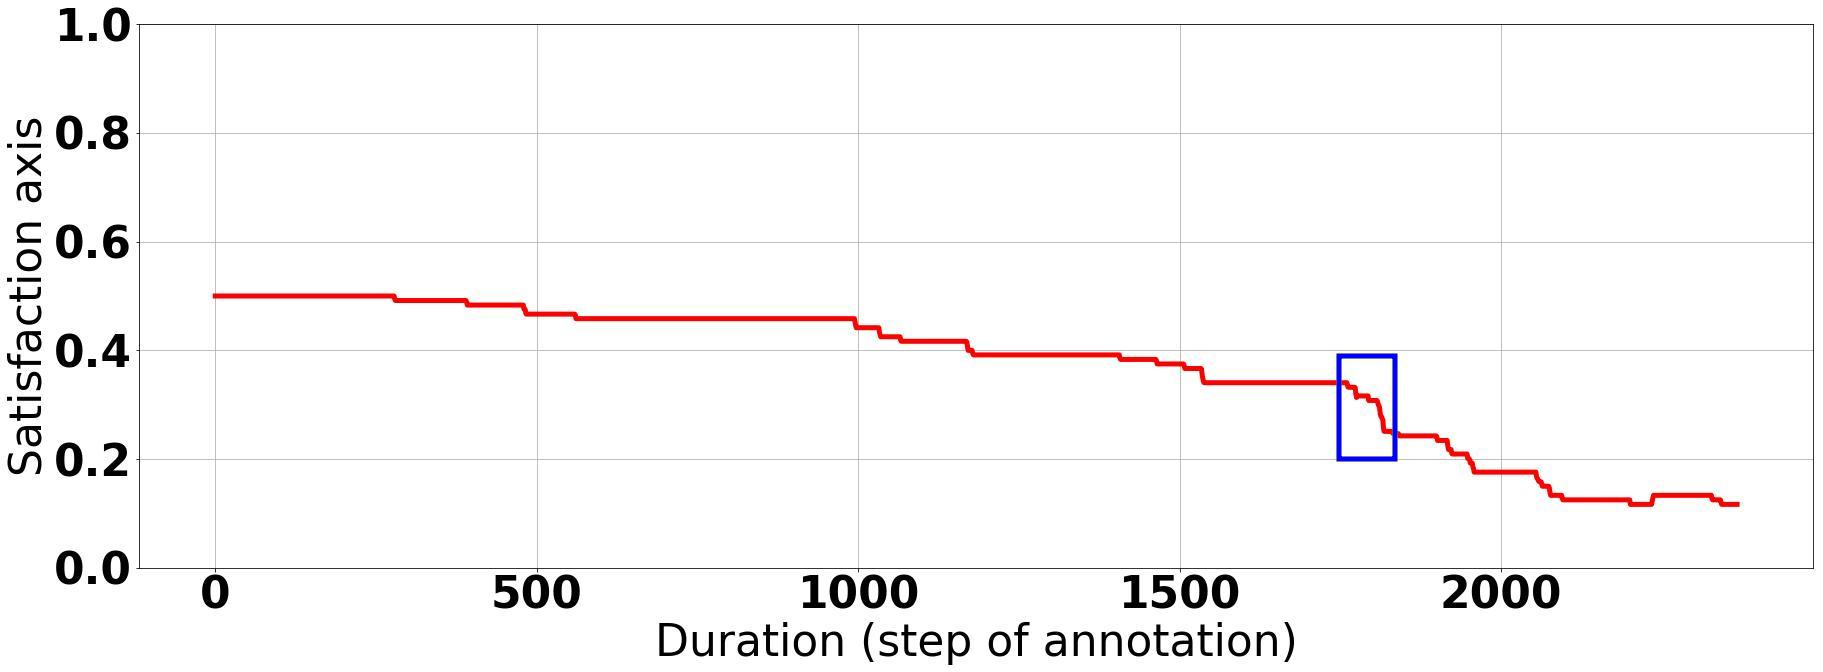
\includegraphics[width=15cm]{./Chapitre7/figures/pic.jpeg}
  \caption{Exemple de segment considéré comme une pente de frustration. Le rectangle bleu correspond au segment de pente de frustration.}
  \label{fig:pente}
\end{figure}


Une fois cet élément d'analyse mis en place, nous avons extrait les 166 transcriptions correspondant à ces pentes de frustration, en prenant du contexte gauche et droit à hauteur de deux secondes. Des exemples de segments ainsi récupérés sont indiqués dans le tableau~\ref{tab:phrasesPente}. On peut voir des mots issus de vocabulaire négatif comme \textit{perds mon temps} et \textit{avez fait l'erreur}, ainsi que des constructions spécifiques : des répétitions et une grande insistance sur le sujet avec des \textit{moi je} notamment.

\subsubsection{Utilisation de TF-IDF}

\begin{table}[h]
    \centering
    \begin{tabular}{|l|}
         \hline
         parce que d'abord je perds du temps alors moi je \\
         chacun son tour si vous voulez donc moi ce que je vous dis c'est que le véhicule \\
        ce que je me j'essaie de faire depuis au moins deux semaines \\
        vais faire appel à mon assistance juridique parce que \\
        vais tout supprimer et puis c'est tout \\
        juste pour dire en fait voilà il me faut ça point barre c'est ça \\
        putain mais visiblement c'est ça \\
        abonnement pour rien du tout \\
        c'est vous qui avez fait l'erreur donc je veux ma carte \\
        alors ça veut dire qu'il faut que je paie une blinde \\
        j'en ai vraiment besoin je comprends pas \\
         \hline
    \end{tabular}
    \caption{Exemple de transcription de segments considérés comme pente de frustration.}
    \label{tab:phrasesPente}
\end{table}


A partir de ces segments, nous avons conduit une analyse statistique. En utilisant TF-IDF, nous avons analysé les mots, les bi-mots et les tri-mots les plus pertinents. Nous avons ensuite utilisé le résultat de cette fonction pour construire des nuages de mots, illustrés dans la Figure~\ref{fig:nuageMot}. Comme nous pouvons le voir, il y a une forte représentation du \textit{je} dans les bi et tri-mots. On observe également beaucoup de tournures négatives (\textit{c'est pas, même pas, je sais pas, je suis pas, c'est pas possible}...) ainsi que des répétitions du mais. De plus, on retrouve des mots et des tournures a polarité négatives (\textit{un problème, gros soucis, déposer plainte, j'ai fait opposition, je suis débile, bêtise...}) et des références à des notions temporelles (\textit{dix jours, tous les mois, ce week-end...}). Néanmoins, si nous réalisons les mêmes opérations sur les autres segments, ne correspondant pas aux pentes de frustration, on peut retrouver une grande partie de ces observations.

\begin{figure}[h]
  \centering
  \begin{minipage}[b]{0.49\linewidth}
      \center
      \centerline{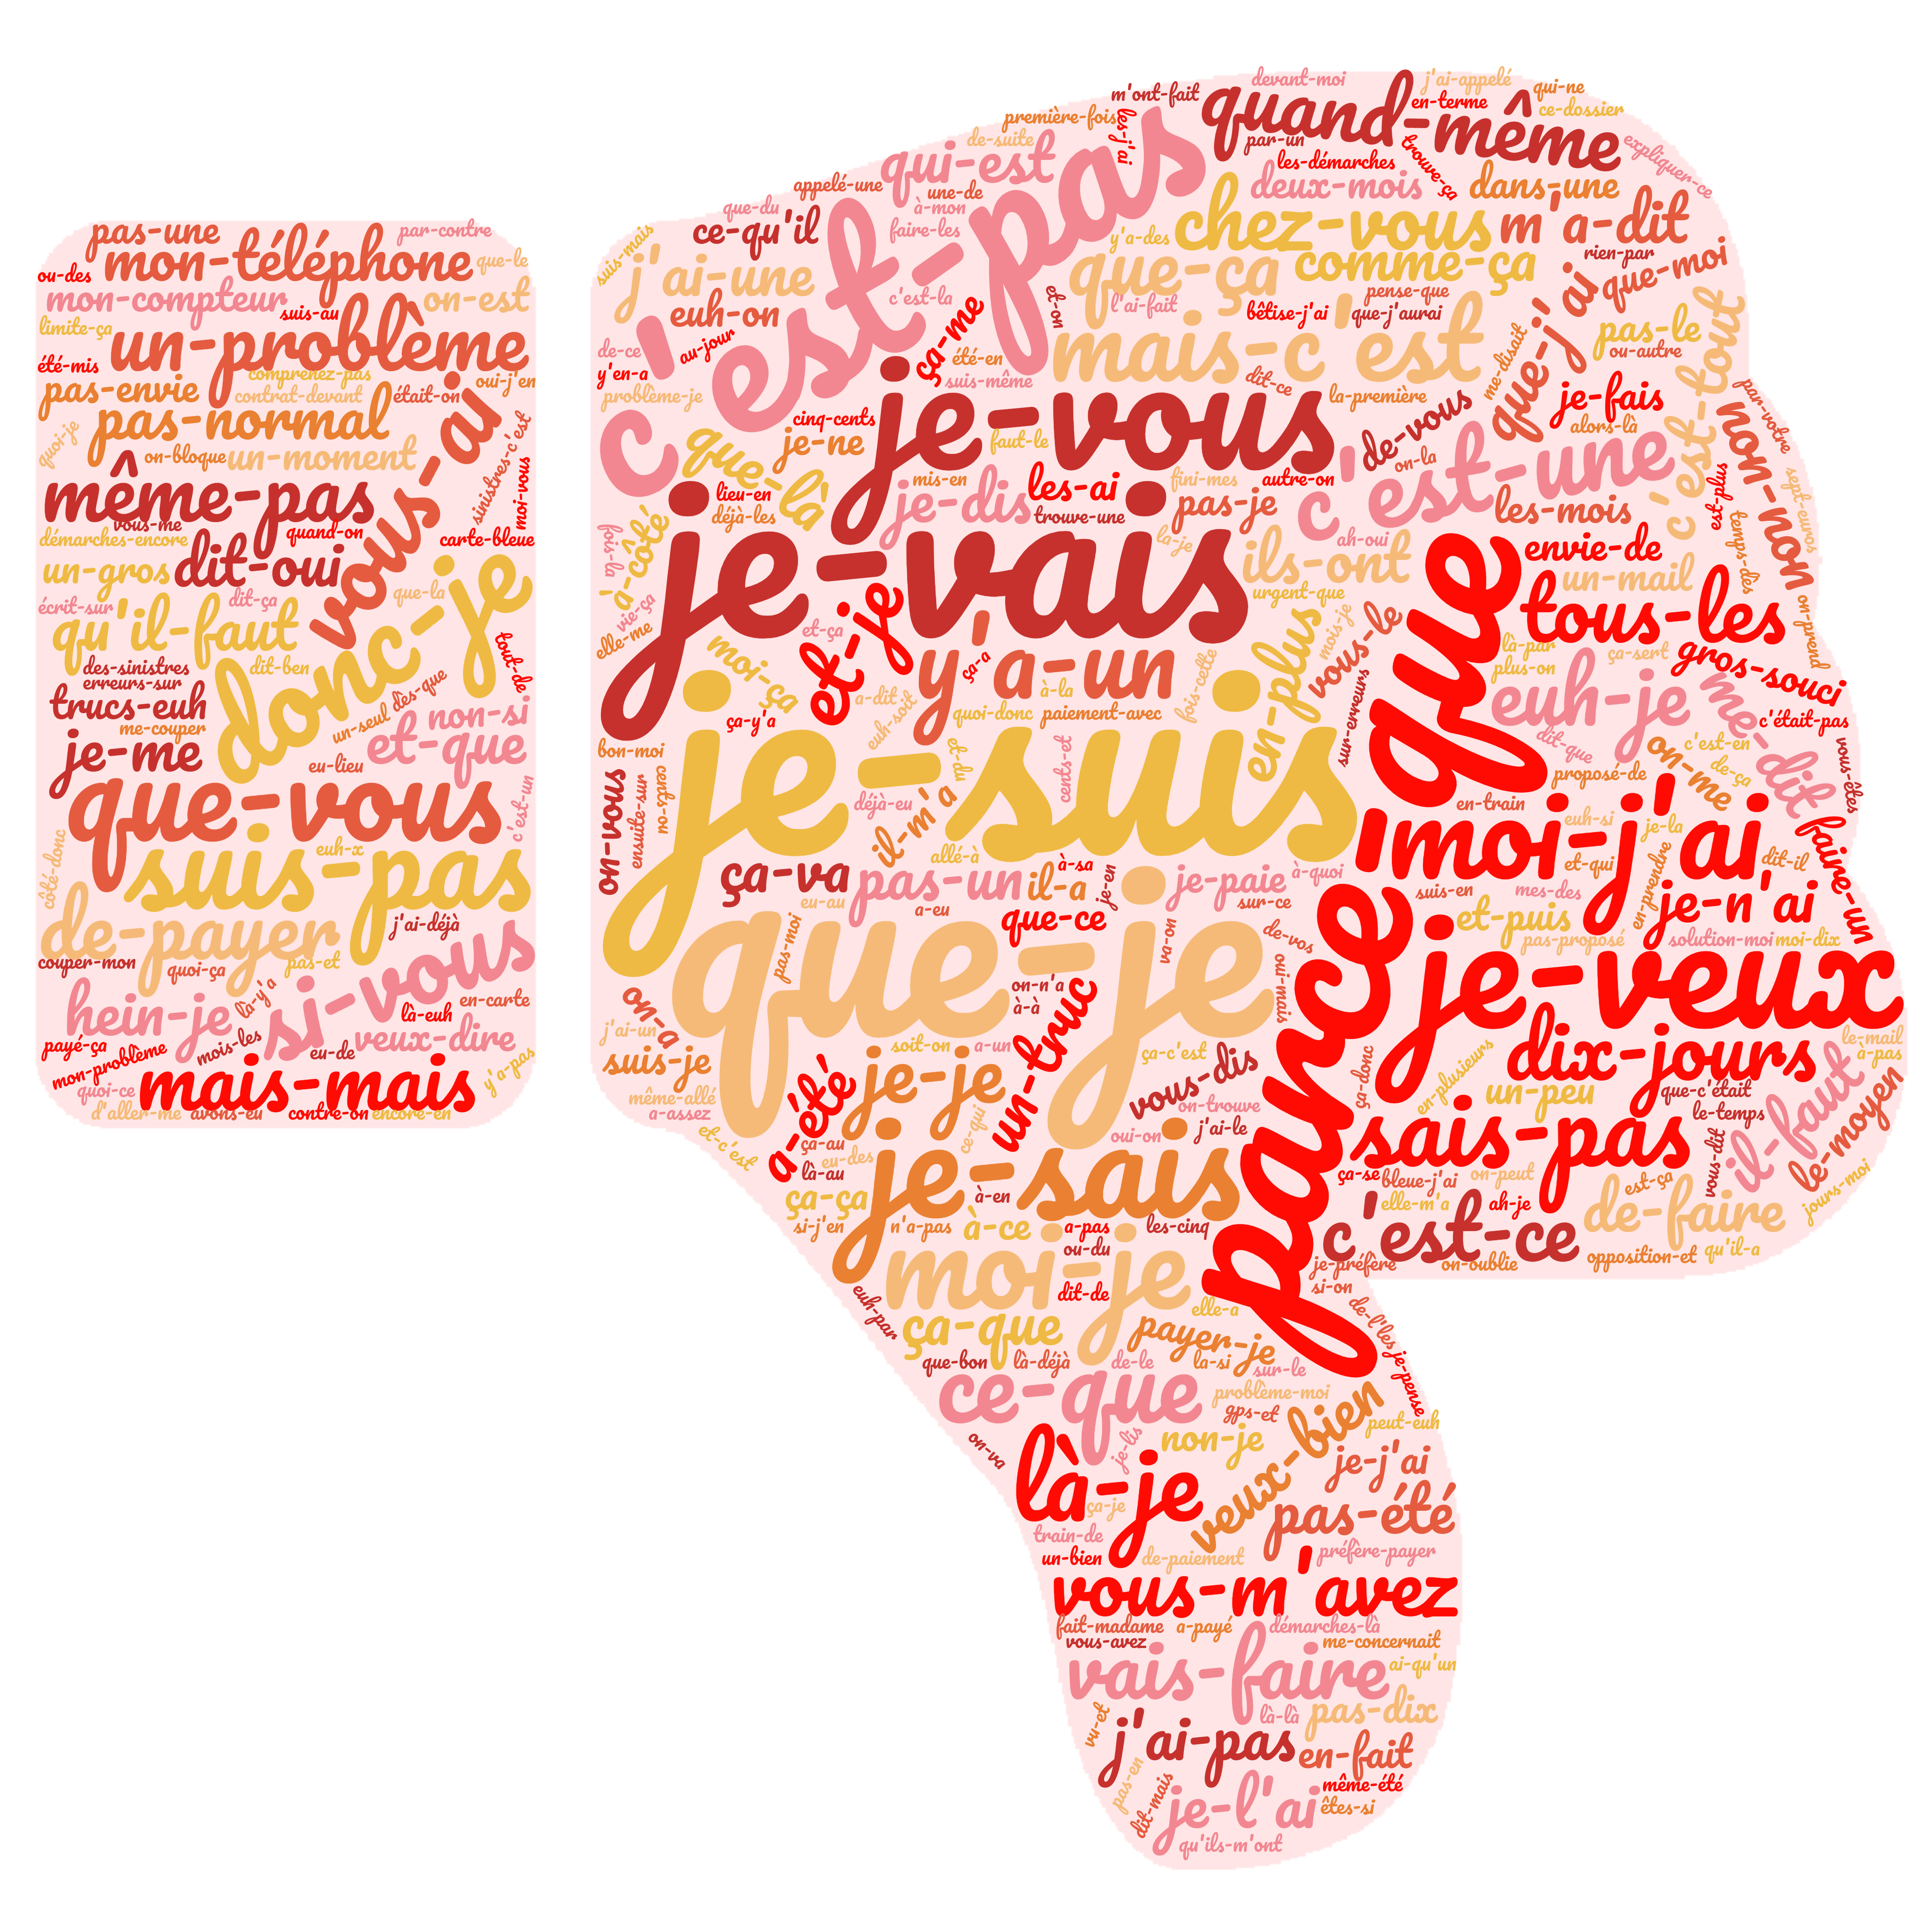
\includegraphics[width=8cm]{./Chapitre7/figures/bigram_pentu.png}}
  \end{minipage}
  \begin{minipage}[b]{0.49\linewidth}
      \center
      \centerline{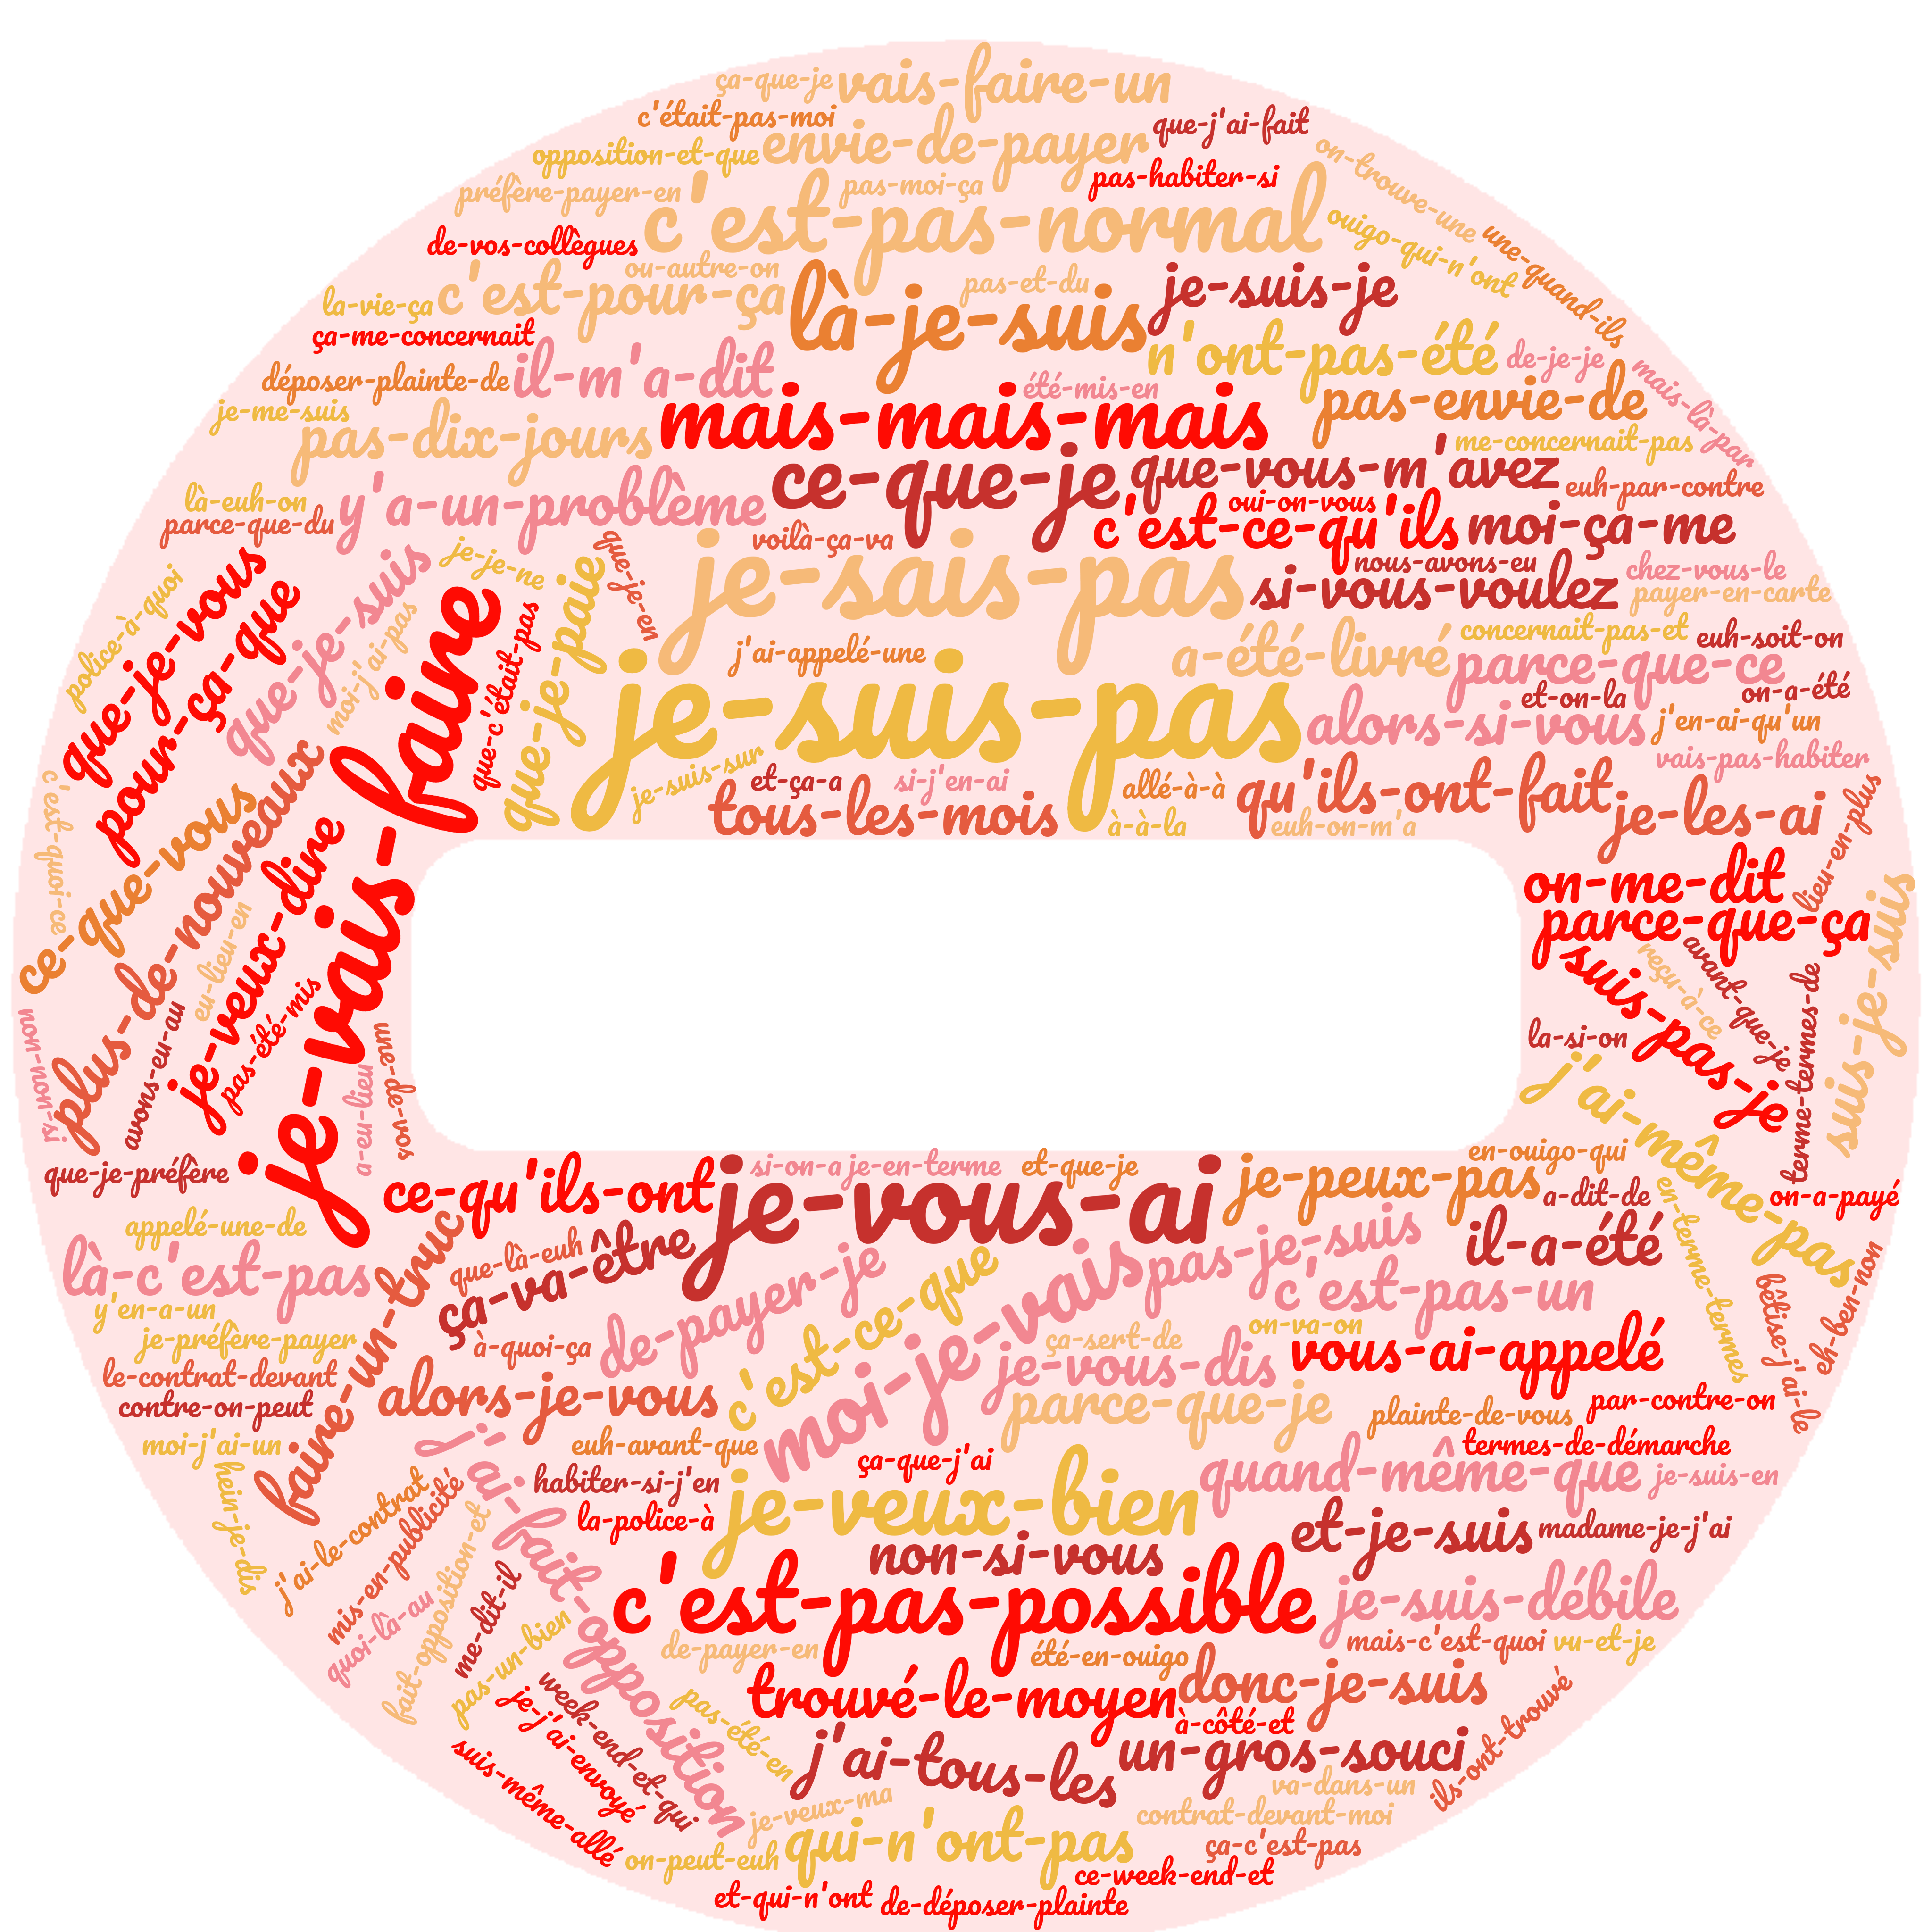
\includegraphics[width=8cm]{./Chapitre7/figures/trigram_pentu.png}}
  \end{minipage}
    \caption{Nuages de mots construits à partir des occurences de bi-mots (gauche) et tri-mots (droite) extraites des transcriptions des segments de pentes de frustration.}
    \label{fig:nuageMot}
\end{figure}


Nous avons également cherché au niveau de la syntaxe s'il y avait des schémas reconnaissables dans l'expression de la satisfaction. Pour cela, nous avons utilisé l’outil Macaon afin de faire un POS-tagging des segments. À partir du résultat de cette opération, nous pouvons extraire le rôle de chaque mot dans les segments mais nous n'arrivons pas à tirer des conclusions de ces observations. %(sujet, verbe, complément...). Nous avons alors utilisé un TF-IDF pour analyser les mots, bi-mots et tri-mots. Le tableau~\ref{tab:posPic} recense les différentes structures de segments que nous avons relevé. Nous n'arrivons pas à tirer des conclusions de ce classement.

%\begin{table}[h]
    \centering
    \begin{tabular}{|l|}
         \hline
          ROOT OBJ MOD SUJ OBJ P_OBJ OBJ ROOT ROOT ROOT
          ROOT DET ROOT ROOT SUJ OBJ COORD SUJ \textbf{DISFLINK} OBJ SUJ P_OBJ DEP_COORD COORD OBJ DET OBJ
          ROOT \textbf{DISFLINK}
          ROOT ROOT \textbf{DISFLINK} DET ROOT SUJ MOD MOD_REL MOD MOD
          \textbf{DISFLINK}
          ROOT OBJ OBJ MOD P_OBJ DET OBJ COORD P_OBJ DEP_COORD MOD MOD OBJ SUJ SUJ AUX OBJ
          ROOT ROOT SUJ OBJ MOD AFF OBJ P_OBJ DET OBJ COORD DET DEP_COORD
          ROOT ROOT SUJ OBJ SUJ ROOT SUJ ROOT OBJ OBJ OBJ DET OBJ ROOT OBJ ROOT
          ROOT MOD OBJ \textbf{DISFLINK} MOD OBJ AFF OBJ OBJ
          ROOT ROOT \textbf{DISFLINK} AFF DEP_COORD \textbf{DISFLINK}
          ROOT ROOT OBJ MOD OBJ MOD OBJ SUJ
          DET OBJ OBJ AFF OBJ OBJ OBJ \textbf{DISFLINK} \textbf{DISFLINK} MOD MOD ROOT
          AUX ROOT COORD DET SUJ AUX DEP_COORD P_OBJ OBJ
          ROOT \textbf{DISFLINK} OBJ ROOT MOD COORD DEP_COORD OBJ DET SUJ DEP_COORD
          ROOT OBJ OBJ ROOT DET OBJ MOD MOD ROOT
          ROOT MOD OBJ COORD ROOT DEP_COORD MOD
          ROOT \textbf{DISFLINK} \textbf{DISFLINK} ROOT
         \hline
    \end{tabular}
    \caption{Part-Of-Speech structure des segments correspondant aux pics de frustration.}
    \label{tab:posPic}
\end{table}


Comme nous n'arrivons pas à dégager clairement des caractéristiques communes à ces segments, nous avons pensé à utiliser le machine learning pour regrouper les segments en classes, et donc nous permettre de discerner les différences entre les classes. Ainsi nous pourrons peut-être décrire des marqueurs de frustration.

\subsubsection{Classification des segments de pente de frustration}
Comme nous n'avons pas de classes définies, nous avons fait le choix d'une classification non supervisée. Pour être cohérent avec le nombre limité de segments émotionnels (166), nous avons utilisé un classifieur de type kmeans avec k=3. Nous avons classifié les mots, bi-mots et tri-mots suivant ces 3 classes. Nous avons effectué une analyse en composantes principales afin de permettre la visualisation sur les deux premières composantes de nos classes, comme l'illustre la Figure~\ref{fig:kmeans}.

\begin{figure}[h]
  \centering
  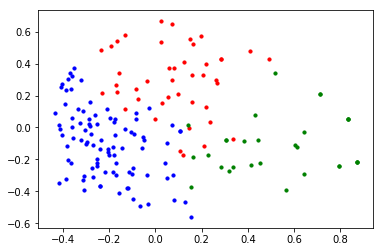
\includegraphics[width=8cm]{./Chapitre7/figures/datakmeans.png}
  \caption{Visualisation des données de segments émotionnels opérée par une pca, sur laquelle une classification de type kmeans (k=3) est effectuée.}
  \label{fig:kmeans}
\end{figure}


Nous avons ensuite utilisé des TF-IDF, dont nous avons expliqué le fonctionnement au chapitre~\ref{chapitre3}, sur les segments de chaque classe pour dégager des tendances. Les résultats sur les bi-mots et les tri-mots sont relatés dans le tableau~\ref{tab:kmeans}. Nous n'avons pas trouvé de caractéristiques bien saillantes dans ces classes qui permettraient de les dissocier à coup sûr. S'il fallait extrapoler, le premier cluster semble contenir des conversations en rapport avec les mutuelles; le deuxième cluster semble plutôt concerner des relances ou des clients qui ont déjà appelés; et le dernier cluster semble être peuplé de litiges de contrat (notamment de l'énergie).

\begin{table}[]
\centering
\begin{tabular}{|l|l|l|}
 \hline
 cluster 1 &cluster 2 &cluster 3 \\
 \hline
 au revoir 	& du tout 	&que je \\
 affiche bon 	& en fait 	& parce que \\
euh attendez 	& en ai 	& je vous \\
 eu lieu 	& qu on 	& je ai \\
la vie 	& je ai 	&ce que \\
 monsieur au 	& du coup 	& je suis \\
 et on 	&ai pas 	& si vous \\
 plus la 	&je comprends 	&que vous \\
 quatre fois 	& comprends pas 	&pas de \\
euh quatre 	&accord euh 	& et je \\
la fille 	&pas accord 	& ai envoyé \\
 je suis 	& est pas 	&moi ai \\
euh je 	& on fait 	& mais mais \\
il été 	& ils ont 	& ai appelé \\
 été livré 	& je vous 	&quand même \\
 personne ne 	&ont fait 	& je vais \\
 on sait 	&on est 	&vous comprenez \\
 ai appelé 	& fait madame 	&ai pas \\
 la rubrique 	& ai fait 	& suis je \\
lisez le 	& je peux 	&que ça \\
les choses 	&peux pas 	& est pas \\
mon billet 	& fait ça 	& je sais \\
 même allé 	& ce qu 	& donc je \\
 procès verbal 	&fait est 	& je veux \\
 la commande 	& ça fait 	&moi je \\
 faire les 	&ai ras 	&est ça \\
imprimer mon 	&ras le 	& vous voulez \\
 deux fois 	&le bol 	&que là \\
ai euh 	&un petit 	&que ai \\
 allé la 	& petit peu 	& alors que \\
annuler la 	&coup juste 	&je viens \\
assure votre 	&juste qu 	&élégant mais \\
 choses quoi 	&moi en 	&souci là \\
 de vous 	&est ça 	&mais bon \\
donc euh 	&pas du 	& viens appeler \\
 ils demandent 	& pour rien 	& là même \\
donc votre 	& rien du 	& je te \\
%  au revoir &0.027166	& du tout &0.030727	&que je &0.035652\\
%  affiche bon &0.014706	& en fait &0.028779	& parce que &0.032408\\
% euh attendez &0.014706	& en ai &0.027737	& je vous &0.026586\\
%  eu lieu &0.014706	& qu on &0.027021	& je ai &0.025469\\
% la vie &0.014706	& je ai &0.022723	&ce que &0.021531\\
%  monsieur au &0.013391	& du coup &0.019896	& je suis &0.020211\\
%  et on &0.012938	&ai pas &0.019834	& si vous &0.018290\\
%  plus la &0.010399	&je comprends &0.017689	&que vous &0.017569\\
%  quatre fois &0.010399	& comprends pas &0.017689	&pas de &0.016381\\
% euh quatre &0.010399	&accord euh &0.017678	& et je &0.016240\\
% la fille &0.010399	&pas accord &0.017678	& ai envoyé &0.016013\\
%  je suis &0.010307	& est pas &0.016991	&moi ai &0.014111\\
% euh je &0.010099	& on fait &0.016923	& mais mais &0.013664\\
% il été &0.009804	& ils ont &0.016289	& ai appelé &0.013534\\
%  été livré &0.009804	& je vous &0.016268	&quand même &0.013403\\
%  personne ne &0.009632	&ont fait &0.015485	& je vais &0.013385\\
%  on sait &0.008880	&on est &0.014932	&vous comprenez &0.013015\\
%  ai appelé &0.008864	& fait madame &0.014918	&ai pas &0.012487\\
%  la rubrique &0.008490	& ai fait &0.014918	& suis je &0.012430\\
% lisez le &0.008490	& je peux &0.014684	&que ça &0.012165\\
% les choses &0.008490	&peux pas &0.014684	& est pas &0.011947\\
% mon billet &0.008490	& fait ça &0.014575	& je sais &0.011900\\
%  même allé &0.008490	& ce qu &0.014359	& donc je &0.011601\\
%  procès verbal &0.008490	&fait est &0.014359	& je veux &0.011253\\
%  la commande &0.008490	& ça fait &0.014110	&moi je &0.011100\\
%  faire les &0.008490	&ai ras &0.014014	&est ça &0.011097\\
% imprimer mon &0.008490	&ras le &0.014014	& vous voulez &0.011065\\
%  deux fois &0.008490	&le bol &0.014014	&que là &0.010637\\
% ai euh &0.008490	&un petit &0.013868	&que ai &0.010344\\
%  allé la &0.008490	& petit peu &0.013868	& alors que &0.010280\\
% annuler la &0.008490	&coup juste &0.013549	&je viens &0.010248\\
% assure votre &0.008490	&juste qu &0.013549	&élégant mais &0.010248\\
%  choses quoi &0.008490	&moi en &0.013147	&souci là &0.010248\\
%  de vous &0.008490	&est ça &0.013095	&mais bon &0.010248\\
% donc euh &0.008490	&pas du &0.013023	& viens appeler &0.010248\\
%  ils demandent &0.008490	& pour rien &0.013023	& là même &0.010248\\
% donc votre &0.008490	& rien du &0.013023	& je te &0.009816\\
% euh ai &0.008490	& euh bon &0.013023	& ça va &0.009732\\
% euh donc &0.008490	& abonnement pour &0.013023	& vous ai &0.009701\\
% euh imprimer &0.008490	&tout euh &0.013023	&vais faire &0.009654\\
% relancer euh &0.008490	&comment on &0.012810	& ça ça &0.009608\\
%  hospitalisée deux &0.008490	&expliqué comment &0.012810	&alors si &0.009484\\
%  qui annuler &0.008490	&qui expliqué &0.012810	&même que &0.009442\\
%  être hospitalisée &0.008490	&deux jours &0.012431	&donc moi &0.009255\\
% verbal ils &0.008490	& pas envie &0.011997	&pas le &0.009107\\
%  vous relancer &0.008490	&envie de &0.011997	&pas me &0.009024\\
%  voilà euh &0.008490	&de payer &0.011997	&non si &0.008824\\
%  votre lisez &0.008490	& demain eu &0.011180	&et que &0.008768\\
%  de la &0.008458	& pas répondu &0.011180	& je fais &0.008755\\
% qu ils &0.008119	&moi du &0.011180	& il vous &0.008739\\
 \hline
\end{tabular}
\caption{Classification bi-mots des segments émotionnels correspondant aux pentes de frustration sur laquelle nous avons appliqué un TF-IDF.}
\label{tab:kmeans}
\end{table}


Nous avons donc fait le choix de nous tourner vers un linguiste, afin de collaborer sur l'analyse des transcriptions et retrouver des marqueurs humainement identifiables de la frustration.


\subsection{Analyses conduites par un linguiste}
Dans cette section, nous avons l'intention de fournir des éléments qui pourraient expliquer l'importance de la linguistique pour retrouver la satisfaction ou la frustration.
Cette analyse a été faite sur 13 conversations sélectionnées afin de couvrir différentes dynamiques de la dimension satisfaction : globalement plates, occurrences de frustration élevée (annotation de l'axe $<$ 0.4) et occurrences de satisfaction fortement décroissante (pente de frustration).
L'analyse a été effectuée à l'aide de la transcription automatique, de l'annotation de l'axe de satisfaction de référence et des balises correspondant à \textit{haute frustration} et \textit{pente de frustration}.

Notre hypothèse est que la parole frustrée comporte principalement  des accentuations des phénomènes oraux.
Par conséquent, nous avons relevé plus spécifiquement :
\begin{itemize}
    \item Quantité de disfluences,
    \item Hésitations, répétitions, bégaiements,
    \item Importance des auto-coupures définies comme \textit{les points où le flux d'énoncé est rompu}~\cite{Pallaud2019},
    \item Usage des interrogations et des négations,
    \item Preuves sémantiques de frustration ou au moins d'émotions négatives,
    \item Quantité de segments significatifs \textit{vs.} segments sémantiquement vides.
\end{itemize}

Sur la base de ces indices, l'analyse aboutit à différentes observations.
Il existe des marqueurs sémantiques de frustration dans les conversations telles que l'usage de la négation (\textit{ça ne m'amuse pas}, \textit{c'est inadmissible}) : des marqueurs forts (\textit{c'est gonflé}, \textit{putain de ...}) et des marqueurs faibles (\textit{quand même}, \textit{franchement}).
Il semble également que la quantité de segments significatifs, d'auto-ruptures et de disfluences, soit généralement corrélée à de fortes augmentations de frustration. La structure syntaxique des énoncés interrogatifs semble également corrélée à la frustration.

Dans un second temps, nous comptons aller plus loin dans cette analyse avec l'extraction automatique d'indices de la frustration.
Bien entendu, passer d'une extraction manuelle à une extraction automatisée en fonction du temps (avec un pas de 250~ms) implique de faire des choix dans la définition des indices.
%\textcolor{red}{Ici il faudrait préciser que c'est une extraction en fonction de temps avec un pas de 250ms ? dans le papier IEEE: "All the occurrences of features summarized in Table VII are synchronized in time together with the annotated satisfaction reference."}
En essayant de modéliser la quantité de segments significatifs, nous extrayons les balises POS à l'aide de MACAON~\cite{Nasr2011} directement à partir de transcriptions automatiques et calculons le nombre de verbes et de noms que l'on met en relation avec le temps.
Pour capturer les autres indices, nous avons décidé d'extraire automatiquement les sept caractéristiques mentionnées dans le tableau ~\ref{tab:ex_features}.

\begin{table}[]
    \centering
    \begin{tabular}{|l|c|}
      \hline
    \textbf{Caractéristiques} & \textbf{Nombre d'occurrences} \\\hline
    Répétition d'un mot (deg1)     & 26 \\
    Répétitions de deux mots (deg2) & 4\\
    Pauses dans le discours (\textit{euh, bah, hein, eh, etc.}) & 22\\
    Marqueurs forts (\textit{important, inquiet, scandaleux, etc.}) & 14\\
    Marqueurs faibles (\textit{quand même, franchement, etc.}) & 3\\
    Négations (\textit{pas, ne, n'}) & 30\\
    \textit{c'est} & 44\\ \hline
    nombre de mots dans \textit{lettre recommandée} & 1050 \\
    nombre de segment de parole dans \textit{lettre recommandée} & 152 \\ \hline
    \end{tabular}
    \caption{Sept caractéristiques et leur nombre d'occurrences permettent de modéliser les indices supposés être responsables de la frustration dans les conversations. Le nombre total de mots et de segments de parole de la conversation appelée \textit{lettre recommandée}, sont également indiqués.}
    \label{tab:ex_features}
\end{table}


L'idée n'est pas de fournir une analyse exhaustive sur l'ensemble des données mais de fournir quelques indices explicables. Nous nous concentrons ici sur l'analyse approfondie d'une seule conversation que nous appelons \textit{lettre certifiée}. Toutes les occurrences des caractéristiques résumées dans Table~\ref{tab:ex_features} sont synchronisées dans le temps avec la référence de satisfaction annotée.

\begin{figure}
    \centering
    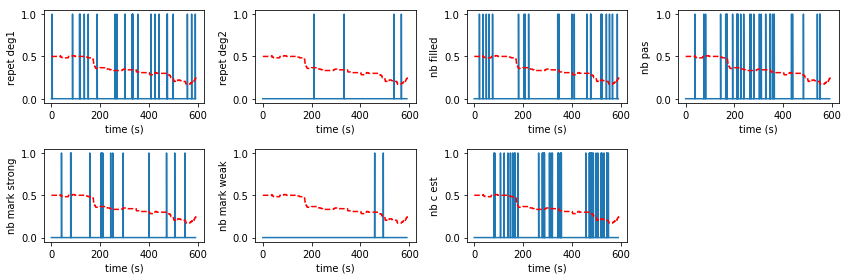
\includegraphics[width=\textwidth]{./Chapitre7/figures/ex_dynamic.png}
    \caption{Analyse dynamique de la frustration de la conversation appelée \textit{lettre certifiée}. Le nombre d'occurrences des sept caractéristiques linguistiques est tracé par rapport au temps. La référence de l'axe de satisfaction est représentée par la ligne en pointillée rouge.}
    \label{fig:ex_dynamic}
\end{figure}


Les quantités de verbes et de noms ne donnent pas d'information pertinente et ne sont pas représentés ici. L'analyse linguistique dynamique est présentée sur la Fig.~\ref{fig:ex_dynamic}. La conversation \textit{lettre certifiée} a été annotée avec une forte baisse de satisfaction avant 200~sec. La transcription automatique obtenue juste avant cette chute est donnée dans le Tableau~\ref{tab:ex_transcription}. Juste avant la chute, les occurrences de répétition de mots simples et de \textit{c'est} sont importantes, alors qu'après la chute, le nombre de pauses remplies par des interjections (\textit{euh, bah, hein, eh}, etc...) et de marqueur de négation (\textit{pas}) augmente. On remarque également qu'un marqueur fort (\textit{réclamation}) se produit juste avant la chute, signifiant probablement que ce mot spécifique induit la perception d'une frustration notable.

\begin{table}[h]
    \centering
    \begin{tabular}{|p{0.80\textwidth}|}
      \hline
    - \textit{voilà} et \underline{la deuxième lettre}  // c'est pareil \textit{mais bon} \underline{cette lettre}  // \underline{elle} est où maintenant… pas comprendre pourquoi on n'a pas retiré \underline{la lettre}... \underline{la deuxième lettre}  // c'est pareil \textit{mais} \underline{elle} venait d'où  // \underline{cette lettre}... c’était \underline{qui}  // \underline{qui} a envoyé \underline{cette lettre}... parce que c'est important  // on est une société  // nous… \underline{quand on sait pas qui c'est} // ... \underline{comment on peut savoir qui c'est} \textit{ouais mais} \underline{\textbf{ça va pas du tout}} \textit{hein} \underline{\textbf{ça va pas du tout}}  // \underline{ça}
    \\ \hline
    \end{tabular}
    \caption{Extrait (137 - 166~sec.) de la conversation \textit{lettre certifiée}. Disfluences: \textit{italic}; Hesitations, bégaiements: \underline{underline}; Traces Semantiques de la frustration: \textbf{bold}; auto-coupures: //}
    \label{tab:ex_transcription}
\end{table}


Dans le corpus AlloSat, l'information émotionnelle semble résider davantage dans les mots que dans le contenu prosodique et acoustique. Dans ces données, l'expression de la frustration est principalement liée à l'accentuation des phénomènes oraux : le contenu sémantique et surtout les auto-coupures, les disfluences, les hésitations et les répétitions.

\section{Considération du genre}
Nous avons voulu conduire une analyse genrée des échanges entre les clients et les conseillers. En effet, nous voulons voir si le genre a un impact sur la frustration et son expression dans notre corpus. Pour ce faire, nous avons extrait les pairs clients-conseillers dont nous avions les informations, soit 81 conversations sur les 303. En effet, le corpus ne comportant pas de données sur le conseiller, il s'agit de données confidentielles soumises à la RGDP, qui explique que la plupart des métadonnées des conversations ne sont pas conservées par l'entreprise.

\begin{table}[]
\centering
\begin{tabular}{|l l|l|l|}
 \hline
 Client	&Conseiller	&Nombre de conversation	&Pente de frustration présent \\
 \hline
femme	&femme	&38	&9	\\
homme	&homme	&5	&0	\\
femme	&homme	&17	&5	\\
homme	&femme	&21	&7	\\
 \hline
\end{tabular}
\caption{Présence de pentes de frustration en fonction du genre de la pair d'interlocuteur.}
\label{tab:genre}
\end{table}


Nous avons voulu mettre l'accent sur les conversations portant des pentes de frustration tel que définis dans ce chapitre. Comme nous pouvons le voir dans le tableau~\ref{tab:genre}, il n'y a pas assez de données pour donner une quelconque conclusion significative. Dans la Figure~\ref{fig:genre}, nous avons l'impression que les hommes sont plus énervés quand ils ont une femme en tant qu'interlocutrice et que la frustration est plus présente sur les pairs hétérogènes.

\begin{figure}[h]
  \centering
  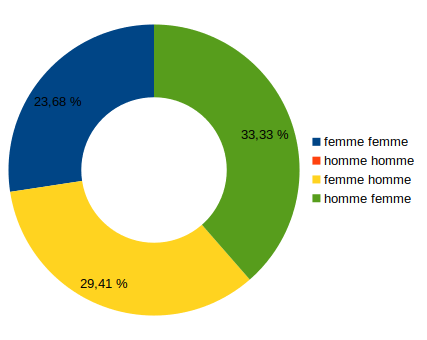
\includegraphics[width=10cm]{./Chapitre7/figures/genre.png}
  \caption{Visualisation du pourcentage de conversations contenant des pics de frustration en fonction du genre de la pair d'interlocuteurs. Le couple homme-homme n'apparait pas puisqu'il n'y a pas de conversations avec un pic de frustration pour cette pair d'interlocuteurs dans les 81 conversations considérées.}
  \label{fig:genre}
\end{figure}


 Il serait intéressant de conduire une étude plus large sur l'impact du genre des interlocuteurs sur l'expression de la frustration.

\section{Conclusion}
Dans ce dernier chapitre de contribution, nous avons souhaité prendre du recul sur nos travaux et expliquer nos résultats. Nous avons tout d'abord discuté de l'utilisation d'une annotation moyennée comme référence à nos systèmes de reconnaissance et plus largement de la pertinence de ce protocole qui est très largement adopté au sein de la communauté scientifique pour les tâches ayant une part non négligeable de subjectivité. Nous nous sommes ensuite concentrés sur la modalité linguistique de notre corpus, à savoir les transcriptions automatiques des conversations, et nous avons essayé de mettre en lumière les facteurs expliquant la très bonne performance des systèmes de reconnaissance appris à partir du texte. Enfin nous avons considéré rapidement l'impact du genre sur la frustration.

Nous pouvons conclure qu'il est difficile de statuer sur des marqueurs linguistiques de la frustration. En effet, en tant qu'humain, nous ressentons bien cette frustration dans le texte, sans pour autant pouvoir définir des marqueurs clairs et universels de cette émotion. Nous pouvons néanmoins souligner la présence des disfluences, des auto-coupures et des bégaiements comme des marqueurs pouvant alerter sur une potentielle frustration.

%\clearemptydoublepage
%\backmatter
%\chapter*{Conclusion}
\addcontentsline{toc}{chapter}{Conclusion}
\chaptermark{Conclusion}


Lorem ipsum dolor sit amet, «~consectetuer~» adipiscing elit. Maecenas fermentum, elit non lobortis cursus, orci velit suscipit est, id mollis turpis mi eget orci. Ut aliquam sollicitudin metus. Mauris at sapien sed sapien congue iaculis. Nulla lorem urna, bibendum id, laoreet iaculis, nonummy eget, massa. Phasellus ullamcorper commodo velit. Class aptent taciti sociosqu ad litora torquent per «~conubia nostra~», per inceptos hymenaeos. Phasellus est. Maecenas felis augue, gravida quis, porta adipiscing, iaculis vitae, felis. Nullam ipsum. Nulla a sem ac leo fringilla mattis. Phasellus egestas augue in sem. Etiam ac enim non mauris ullamcorper scelerisque. In wisi leo, malesuada vulputate, tempor sit amet, facilisis vel, velit. Mauris massa est, sodales placerat, luctus id, hendrerit a, urna. Nullam eleifend pede eget odio. Duis non erat. Nullam pellentesque.


% Chapitre pour la bibliographie
% Bibliography chapter
\clearemptydoublepage
\phantomsection % To have a correct link in the table of contents
\addcontentsline{toc}{chapter}{Bibliographie}

\printbibliography

% nocite: Pour citer la totalit\'{e} des r\'{e}f\'{e}rences contenues dans le fichier biblio
% nocite: In order to cite all the references included biblio
%\nocite{*}
%\printbibliography[heading=primary,keyword=primary]
%\newpage
%\nocite{*}
%\printbibliography[heading=secondary,keyword=secondary]

% \clearemptydoublepage
% \chapter{Appendix}
\section{Guide d'installation et de configuration de CARMA}
\label{ap:guideInstall}
\include[pages=-]{guideInstall.pdf}

\section{Guide d'annotations}
\label{ap:guidelines}
\include[pages=-]{guidelines.pdf}

\section{End User Licence Agreement}
\label{ap:eula}
\include[pages=-]{eula.pdf}




\clearemptydoublepage
% Pour avoir la quatrième de couverture sur une page paire
% To have the back cover on an even page
\cleartoevenpage[\thispagestyle{empty}]
\markboth{}{}
% Plus petite marge du bas pour la quatrième de couverture
% Shorter bottom margin for the back cover
\newgeometry{inner=30mm,outer=20mm,top=40mm,bottom=20mm}

%insertion de l'image de fond du dos (resume)
%background image for resume (back)
\backcoverheader

% Switch font style to back cover style
\selectfontbackcover{ % Font style change is limited to this page using braces, just in case

\titleFR{titre (en fran\c cais)..............}

\keywordsFR{de 6 mots clefs}

\abstractFR{Eius populus ab incunabulis primis ad usque pueritiae tempus extremum, quod annis circumcluditur fere trecentis, circummurana pertulit bella, deinde aetatem ingressus adultam post multiplices bellorum aerumnas Alpes transcendit et fretum, in iuvenem erectus et virum ex omni plaga quam orbis ambit inmensus, reportavit laureas et triumphos, iamque vergens in senium et nomine solo aliquotiens vincens ad tranquilliora vitae discessit.
Hoc inmaturo interitu ipse quoque sui pertaesus excessit e vita aetatis nono anno atque vicensimo cum quadriennio imperasset. natus apud Tuscos in Massa Veternensi, patre Constantio Constantini fratre imperatoris, matreque Galla.
Thalassius vero ea tempestate praefectus praetorio praesens ipse quoque adrogantis ingenii, considerans incitationem eius ad multorum augeri discrimina, non maturitate vel consiliis mitigabat, ut aliquotiens celsae potestates iras principum molliverunt, sed adversando iurgandoque cum parum congrueret, eum ad rabiem potius evibrabat, Augustum actus eius exaggerando creberrime
docens, idque, incertum qua mente, ne lateret adfectans. quibus mox Caesar acrius efferatus, velut contumaciae quoddam vexillum altius erigens, sine respectu salutis alienae vel suae ad vertenda opposita instar rapidi fluminis irrevocabili impetu ferebatur.
Hae duae provinciae bello quondam piratico catervis mixtae praedonum.}



\titleEN{titre (en anglais)..............}

\keywordsEN{de 3 \`{a} 6 mots clefs}

\abstractEN{Eius populus ab incunabulis primis ad usque pueritiae tempus extremum, quod annis circumcluditur fere trecentis, circummurana pertulit bella, deinde aetatem ingressus adultam post multiplices bellorum aerumnas Alpes transcendit et fretum, in iuvenem erectus et virum ex omni plaga quam orbis ambit inmensus, reportavit laureas et triumphos, iamque vergens in senium et nomine solo aliquotiens vincens ad tranquilliora vitae discessit.
Hoc inmaturo interitu ipse quoque sui pertaesus excessit e vita aetatis nono anno atque vicensimo cum quadriennio imperasset. natus apud Tuscos in Massa Veternensi, patre Constantio Constantini fratre imperatoris, matreque Galla.
Thalassius vero ea tempestate praefectus praetorio praesens ipse quoque adrogantis ingenii, considerans incitationem eius ad multorum augeri discrimina, non maturitate vel consiliis mitigabat, ut aliquotiens celsae potestates iras principum molliverunt, sed adversando iurgandoque cum parum congrueret, eum ad rabiem potius evibrabat, Augustum actus eius exaggerando creberrime
docens, idque, incertum qua mente, ne lateret adfectans. quibus mox Caesar acrius efferatus, velut contumaciae quoddam vexillum altius erigens, sine respectu salutis alienae vel suae ad vertenda opposita instar rapidi fluminis irrevocabili impetu ferebatur.
Hae duae provinciae bello quondam piratico catervis mixtae praedonum.}

}

% Rétablit les marges d'origines
% Restore original margin settings
\restoregeometry


\end{document}
